% Options for packages loaded elsewhere
\PassOptionsToPackage{unicode}{hyperref}
\PassOptionsToPackage{hyphens}{url}
%
\documentclass[
]{book}
\usepackage{lmodern}
\usepackage{amssymb,amsmath}
\usepackage{ifxetex,ifluatex}
\ifnum 0\ifxetex 1\fi\ifluatex 1\fi=0 % if pdftex
  \usepackage[T1]{fontenc}
  \usepackage[utf8]{inputenc}
  \usepackage{textcomp} % provide euro and other symbols
\else % if luatex or xetex
  \usepackage{unicode-math}
  \defaultfontfeatures{Scale=MatchLowercase}
  \defaultfontfeatures[\rmfamily]{Ligatures=TeX,Scale=1}
\fi
% Use upquote if available, for straight quotes in verbatim environments
\IfFileExists{upquote.sty}{\usepackage{upquote}}{}
\IfFileExists{microtype.sty}{% use microtype if available
  \usepackage[]{microtype}
  \UseMicrotypeSet[protrusion]{basicmath} % disable protrusion for tt fonts
}{}
\makeatletter
\@ifundefined{KOMAClassName}{% if non-KOMA class
  \IfFileExists{parskip.sty}{%
    \usepackage{parskip}
  }{% else
    \setlength{\parindent}{0pt}
    \setlength{\parskip}{6pt plus 2pt minus 1pt}}
}{% if KOMA class
  \KOMAoptions{parskip=half}}
\makeatother
\usepackage{xcolor}
\IfFileExists{xurl.sty}{\usepackage{xurl}}{} % add URL line breaks if available
\IfFileExists{bookmark.sty}{\usepackage{bookmark}}{\usepackage{hyperref}}
\hypersetup{
  pdftitle={Legislação e normas da educação escolar indígena},
  hidelinks,
  pdfcreator={LaTeX via pandoc}}
\urlstyle{same} % disable monospaced font for URLs
\usepackage{longtable,booktabs}
% Correct order of tables after \paragraph or \subparagraph
\usepackage{etoolbox}
\makeatletter
\patchcmd\longtable{\par}{\if@noskipsec\mbox{}\fi\par}{}{}
\makeatother
% Allow footnotes in longtable head/foot
\IfFileExists{footnotehyper.sty}{\usepackage{footnotehyper}}{\usepackage{footnote}}
\makesavenoteenv{longtable}
\usepackage{graphicx}
\makeatletter
\def\maxwidth{\ifdim\Gin@nat@width>\linewidth\linewidth\else\Gin@nat@width\fi}
\def\maxheight{\ifdim\Gin@nat@height>\textheight\textheight\else\Gin@nat@height\fi}
\makeatother
% Scale images if necessary, so that they will not overflow the page
% margins by default, and it is still possible to overwrite the defaults
% using explicit options in \includegraphics[width, height, ...]{}
\setkeys{Gin}{width=\maxwidth,height=\maxheight,keepaspectratio}
% Set default figure placement to htbp
\makeatletter
\def\fps@figure{htbp}
\makeatother
\setlength{\emergencystretch}{3em} % prevent overfull lines
\providecommand{\tightlist}{%
  \setlength{\itemsep}{0pt}\setlength{\parskip}{0pt}}
\setcounter{secnumdepth}{5}
\usepackage{booktabs}
\ifluatex
  \usepackage{selnolig}  % disable illegal ligatures
\fi
\usepackage[]{natbib}
\bibliographystyle{apalike}

\title{Legislação e normas da educação escolar indígena}
\author{true \and true}
\date{07 de agosto de 2020}

\begin{document}
\maketitle

{
\setcounter{tocdepth}{1}
\tableofcontents
}
\hypertarget{apresentauxe7uxe3o}{%
\chapter{Apresentação}\label{apresentauxe7uxe3o}}

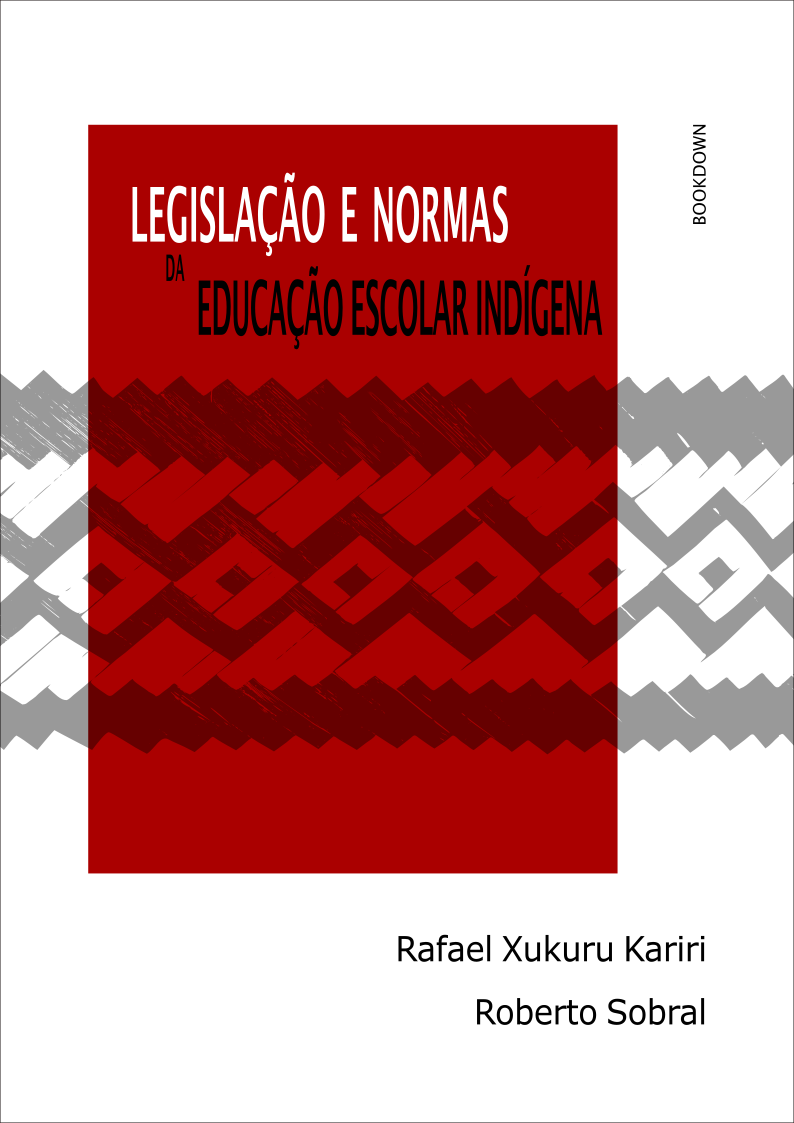
\includegraphics[width=1\linewidth]{C:/Users/joser/OneDrive/2. MEC/2.6._Dados_Estatisticos/legislacao_indigena/legislacao_indigena/capa}

\includegraphics[width=0.7\linewidth]{C:/Users/joser/OneDrive/2. MEC/2.6._Dados_Estatisticos/legislacao_indigena/legislacao_indigena/ficha}

Este é um pequeno compilado de legislações e normas federais relacionadas à EDUCAÇÃO ESCOLAR INDÍGENA.

Nosso objetivo é apresentar um instrumento de consulta, simples e acessível, para todas as pessoas que trabalham na área ou para as que querem conhecer os principais balizadores da organização e do funcionamento da educação escolar indígena no âmbito federal.

Dada as constantes alterações dos atos legais e normativos da área educacional, atualizaremos frequentemente esta publicação a fim de que reflita as modificações mais recentes.

Para eventuais dúvidas, críticas ou sugestões, colocamo-nos à disposição por meio de: \href{mailto:joserobertosobral@gmail.com}{\nolinkurl{joserobertosobral@gmail.com}} / \href{mailto:rafael.silva_19@hotmail.com}{\nolinkurl{rafael.silva\_19@hotmail.com}}.

Rafael Xucuru Kariri

Roberto Sobral

~

~

{Legislação e normas da educação escolar indígena} de Roberto Sobral / Rafael Xukuru Kariri está licenciado com uma Licença Creative Commons - Atribuição 4.0 Internacional.

\hypertarget{intro}{%
\chapter{Diretrizes para a EEI}\label{intro}}

\hypertarget{resoluuxe7uxe3o-cneceb-nuxba-3-de-10-de-novembro-de-1999.}{%
\section{Resolução CNE/CEB nº 3, de 10 de novembro de 1999.*}\label{resoluuxe7uxe3o-cneceb-nuxba-3-de-10-de-novembro-de-1999.}}

\emph{Fixa Diretrizes Nacionais para o funcionamento das escolas indígenas e dá outras providências}

Resolução CNE/CEB nº 3, de 10 de novembro de 1999.

Fixa Diretrizes Nacionais para o funcionamento das escolas indígenas e dá outras providências.

O Presidente da Câmara de Educação Básica do Conselho Nacional de Educação, no uso de suas atribuições regimentais e com base nos artigos 210, § 2º, e 231, caput, da Constituição Federal, nos arts. 78 e 79 da Lei 9.394, de 20 de dezembro de 1996, na Lei 9.131, de 25 de novembro de 1995, e ainda no Parecer CEB 14/99, homologado pelo Senhor Ministro de Estado da Educação, em 18 de outubro de 1999,

RESOLVE:

Art. 1º Estabelecer, no âmbito da educação básica, a estrutura e o funcionamento das Escolas Indígenas, reconhecendo-lhes a condição de escolas com normas e ordenamento jurídico próprios, e fixando as diretrizes curriculares do ensino intercultural e bilíngüe, visando à valorização plena das culturas dos povos indígenas e à afirmação e manutenção de sua diversidade étnica.

Art.2º Constituirão elementos básicos para a organização, a estrutura e o funcionamento da escola indígena:

I - sua localização em terras habitadas por comunidades indígenas, ainda que se estendam por territórios de diversos Estados ou Municípios contíguos;

II -- exclusividade de atendimento a comunidades indígenas;

III -- o ensino ministrado nas línguas maternas das comunidades atendidas, como uma das formas de preservação da realidade sociolingüística de cada povo;

IV -- a organização escolar própria.

Parágrafo Único. A escola indígena será criada em atendimento à reivindicação ou por iniciativa de comunidade interessada, ou com a anuência da mesma, respeitadas suas formas de representação.

Art. 3º Na organização de escola indígena deverá ser considerada a participação da comunidade, na definição do modelo de organização e gestão, bem como:

I- suas estruturas sociais;

II- suas práticas sócio-culturais e religiosas;

III- suas formas de produção de conhecimento, processos próprios e métodos de ensino-aprendizagem;

IV- suas atividades econômicas;

V- a necessidade de edificação de escolas que atendam aos interesses das comunidades indígenas;

VI- o uso de materiais didático-pedagógicos produzidos de acordo com o contexto sócio-cultural de cada povo indígena.

Art 4º As escolas indígenas, respeitados os preceitos constitucionais e legais que fundamentam a sua instituição e normas específicas de funcionamento, editadas pela União e pelos Estados, desenvolverão suas atividades de acordo com o proposto nos respectivos projetos pedagógicos e regimentos escolares com as seguintes prerrogativas:

I -- organização das atividades escolares, independentes do ano civil, respeitado o fluxo das atividades econômicas, sociais, culturais e religiosas;

II -- duração diversificada dos períodos escolares, ajustando-a às condições e especificidades próprias de cada comunidade.

Art. 5º A formulação do projeto pedagógico próprio, por escola ou por povo indígena, terá por base:

I -- as Diretrizes Curriculares Nacionais referentes a cada etapa da educação básica;

II -- as características próprias das escolas indígenas, em respeito à especificidade étnicocultural de cada povo ou comunidade;

III - as realidades sociolíngüística, em cada situação;

IV -- os conteúdos curriculares especificamente indígenas e os modos próprios de constituição do saber e da cultura indígena;

V -- a participação da respectiva comunidade ou povo indígena.

Art. 6º A formação dos professores das escolas indígena será específica, orientar-se-á pelas Diretrizes Curriculares Nacionais e será desenvolvida no âmbito das instituições formadoras de professores.

Parágrafo único. Será garantida aos professores indígenas a sua formação em serviço e, quando for o caso, concomitantemente com a sua própria escolarização.

Art. 7º Os cursos de formação de professores indígenas darão ênfase à constituição de competências referenciadas em conhecimentos, valores, habilidades, e atitudes, na elaboração, no desenvolvimento e na avaliação de currículos e programas próprios, na produção de material didático e na utilização de metodologias adequadas de ensino e pesquisa.

Art. 8º A atividade docente na escola indígena será exercida prioritariamente por professores indígenas oriundos da respectiva etnia.

Art. 9º São definidas, no plano institucional, administrativo e organizacional, as seguintes esferas de competência, em regime de colaboração:

I -- à União caberá legislar, em âmbito nacional, sobre as diretrizes e bases da educação nacional e, em especial:

\begin{enumerate}
\def\labelenumi{\alph{enumi})}
\item
  legislar privativamente sobre a educação escolar indígena;
\item
  definir diretrizes e políticas nacionais para a educação escolar indígena;
\item
  apoiar técnica e financeiramente os sistemas de ensino no provimento dos programas de educação intercultural das comunidades indígenas, no desenvolvimento de programas integrados de ensino e pesquisa, com a participação dessas comunidades para o acompanhamento e a avaliação dos respectivos programas;
\item
  apoiar técnica e financeiramente os sistemas de ensino na formação de professores indígenas e do pessoal técnico especializado;
\item
  criar ou redefinir programas de auxílio ao desenvolvimento da educação, de modo a atender às necessidades escolares indígenas;
\item
  orientar, acompanhar e avaliar o desenvolvimento de ações na área da formação inicial e continuada de professores indígenas;
\item
  elaborar e publicar, sistematicamente, material didático específico e diferenciado, destinado às escolas indígenas.
\end{enumerate}

II - aos Estados competirá:

\begin{enumerate}
\def\labelenumi{\alph{enumi})}
\item
  responsabilizar-se pela oferta e execução da educação escolar indígena, diretamente ou por meio de regime de colaboração com seus municípios;
\item
  regulamentar administrativamente as escolas indígenas, nos respectivos Estados, integrando-as como unidades próprias, autônomas e específicas no sistema estadual;
\item
  prover as escolas indígenas de recursos humanos, materiais e financeiros, para o seu pleno funcionamento;
\item
  instituir e regulamentar a profissionalização e o reconhecimento público do magistério indígena, a ser admitido mediante concurso público específico;
\item
  promover a formação inicial e continuada de professores indígenas.
\item
  elaborar e publicar sistematicamente material didático, específico e diferenciado, para uso nas escolas indígenas.
\end{enumerate}

III - aos Conselhos Estaduais de Educação competirá:

\begin{enumerate}
\def\labelenumi{\alph{enumi})}
\item
  estabelecer critérios específicos para criação e regularização das escolas indígenas e dos cursos de formação de professores indígenas;
\item
  autorizar o funcionamento das escolas indígenas, bem como reconhecê-las;
\item
  regularizar a vida escolar dos alunos indígenas, quando for o caso.
\end{enumerate}

§ 1º Os Municípios poderão oferecer educação escolar indígena, em regime de colaboração com os respectivos Estados, desde que se tenham constituído em sistemas de educação próprios, disponham de condições técnicas e financeiras adequadas e contem com a anuência das comunidades indígenas interessadas.

§ 2º As escolas indígenas, atualmente mantidas por municípios que não satisfaçam as exigências do parágrafo anterior passarão, no prazo máximo de três anos, à responsabilidade dos Estados, ouvidas as comunidades interessadas.

Art.10 O planejamento da educação escolar indígena, em cada sistema de ensino, deve contar com a participação de representantes de professores indígenas, de organizações indígenas e de apoio aos índios, de universidades e órgãos governamentais.

Art. 11 Aplicam-se às escolas indígenas os recursos destinados ao financiamento público da educação.

Parágrafo Único. As necessidades específicas das escolas indígenas serão contempladas por custeios diferenciados na alocação de recursos a que se referem os artigos 2º e 13º da Lei 9424/96.

Art. 12 Professor de escola indígena que não satisfaça as exigências desta Resolução terá garantida a continuidade do exercício do magistério pelo prazo de três anos, exceção feita ao professor indígena, até que possua a formação requerida.

Art. 13 A educação infantil será ofertada quando houver demanda da comunidade indígena interessada.

Art. 14 Os casos omissos serão resolvidos:

I - pelo Conselho Nacional de Educação, quando a matéria estiver vinculada à competência da União;

II - pelos Conselhos Estaduais de Educação.

Art. 15 Esta Resolução entra em vigor na data de sua publicação.

Art. 16 Ficam revogadas as disposições em contrário.

ULYSSES DE OLIVEIRA PANISSET

Presidente da Câmara de Educação Básica

*Este texto não substitui o publicado no Diário Oficial da União, Brasília, 17 de novembro de 1999. Seção 1, p.~19. Republicada em 14 de dezembro de 1999, Seção 1, p.~58, por ter saído com incorreção do original

~

~

\hypertarget{resoluuxe7uxe3o-cneceb-nuxba-5-de-22-de-junho-de-2012.}{%
\section{Resolução CNE/CEB nº 5, de 22 de junho de 2012.}\label{resoluuxe7uxe3o-cneceb-nuxba-5-de-22-de-junho-de-2012.}}

\emph{Define Diretrizes Curriculares Nacionais para a Educação Escolar Indígena na Educação Básica.}

O Presidente da Câmara de Educação Básica do Conselho Nacional de Educação, no uso de suas atribuições legais e de conformidade com o disposto na alínea ``c'' do § 1º do art. 9º da Lei nº 4.024/61, com a redação dada pela Lei nº 9.131/95, na Lei nº 9.394/96, especialmente nos arts. 78 e 79, 26-A, § 4° do art. 26, § 3° do art. 32, bem como no Decreto nº 6.861/2009, e com fundamento no Parecer CNE/CEB nº 13/2012, homologado por Despacho do Senhor Ministro da Educação, publicado no DOU de 15 de junho de 2012,

CONSIDERANDO

O direito a uma educação escolar diferenciada para os povos indígenas, assegurado pela Constituição Federal de 1988; pela Convenção 169 da Organização Internacional do Trabalho (OIT) sobre Povos Indígenas e Tribais, promulgada no Brasil por meio do Decreto nº 5.051/2004; pela Declaração Universal dos Direitos Humanos de 1948 da Organização das Nações Unidas (ONU); pela Declaração das Nações Unidas sobre os direitos dos povos indígenas de 2007; pela Lei de Diretrizes e Bases da Educação Nacional (Lei 9.394/96), bem como por outros documentos nacionais e internacionais que visam assegurar o direito à educação como um direito humano e social;

As Diretrizes Curriculares Nacionais Gerais para a Educação Básica (Parecer CNE/CEB nº 7/2010 e Resolução CNE/CEB nº 4/2010), as Diretrizes Curriculares Nacionais para a Educação Infantil (Parecer CNE/CEB nº 20/2009 e Resolução CNE/CEB nº 5/2009), as Diretrizes Curriculares Nacionais para o Ensino Fundamental (Parecer CNE/CEB nº 11/2010 e Resolução CNE/CEB nº 7/2010), e as Diretrizes Curriculares Nacionais para o Ensino Médio (Parecer CNE/CEB nº 5/2011 e Resolução CNE/CEB nº 2/2012), além de outras que tratam das modalidades que compõem a Educação Básica;

As Diretrizes Nacionais para a Educação em Direitos Humanos definidas no Parecer CNE/CP nº 8/2012;

As recomendações do Parecer CNE/CEB nº 10/2011, que trata da oferta de língua estrangeira nas escolas indígenas de Ensino Médio;

As orientações do Parecer CNE/CEB nº 1/2011 e do Parecer CNE/CEB nº 9/2011, que tratam, respectivamente, de questionamento do Conselho de Educação Escolar Indígena do Amazonas a respeito da transformação do colegiado em órgão normativo, e da proposta de fortalecimento e implementação do regime de colaboração mediante arranjos de desenvolvimento da educação;

As deliberações da I Conferência Nacional de Educação Escolar Indígena, realizada em novembro de 2009, considerada espaço democrático privilegiado de debates e de decisões, com o intuito de celebrar, promover e fortalecer a Educação Escolar Indígena;

As determinações do Decreto nº 6.861/2009, que dispõe sobre a Educação Escolar Indígena e define sua organização em territórios etnoeducacionais;

CONSIDERANDO, finalmente, as contribuições ao texto destas Diretrizes apresentadas pelos participantes dos dois seminários nacionais sobre Diretrizes para a Educação Escolar Indígena, realizados, respectivamente, nos anos de 2011 e 2012 pelo Conselho Nacional de Educação, bem como aquelas enviadas por diversas pessoas e instituições durante o processo de consulta pública,

RESOLVE:

Art. 1º Esta Resolução define as Diretrizes Curriculares Nacionais para a Educação Escolar Indígena na Educação Básica, oferecida em instituições próprias.

Parágrafo único Estas Diretrizes Curriculares Nacionais estão pautadas pelos princípios da igualdade social, da diferença, da especificidade, do bilinguismo e da interculturalidade, fundamentos da Educação Escolar Indígena.

TÍTULO I

DOS OBJETIVOS

Art. 2º As Diretrizes Curriculares Nacionais para a Educação Escolar Indígena na Educação Básica têm por objetivos:

I - orientar as escolas indígenas de educação básica e os sistemas de ensino da União, dos Estados, do Distrito Federal e dos Municípios na elaboração, desenvolvimento e avaliação de seus projetos educativos;

II - orientar os processos de construção de instrumentos normativos dos sistemas de ensino visando tornar a Educação Escolar Indígena projeto orgânico, articulado e sequenciado de Educação Básica entre suas diferentes etapas e modalidades, sendo garantidas as especificidades dos processos educativos indígenas;

III - assegurar que os princípios da especificidade, do bilingüismo e multilinguismo, da organização comunitária e da interculturalidade fundamentem os projetos educativos das comunidades indígenas, valorizando suas línguas e conhecimentos tradicionais;

IV - assegurar que o modelo de organização e gestão das escolas indígenas leve em consideração as práticas socioculturais e econômicas das respectivas comunidades, bem como suas formas de produção de conhecimento, processos próprios de ensino e de aprendizagem e projetos societários;

V - fortalecer o regime de colaboração entre os sistemas de ensino da União, dos Estados, do Distrito Federal e dos Municípios, fornecendo diretrizes para a organização da Educação Escolar Indígena na Educação Básica, no âmbito dos territórios etnoeducacionais;

VI - normatizar dispositivos constantes na Convenção 169, da Organização Internacional do Trabalho, ratificada no Brasil, por meio do Decreto Legislativo nº 143/2003, no que se refere à educação e meios de comunicação, bem como os mecanismos de consulta livre, prévia e informada;

VII - orientar os sistemas de ensino da União, dos Estados, do Distrito Federal e dos Municípios a incluir, tanto nos processos de formação de professores indígenas, quanto no funcionamento regular da Educação Escolar Indígena, a colaboração e atuação de especialistas em saberes tradicionais, como os tocadores de instrumentos musicais, contadores de narrativas míticas, pajés e xamãs, rezadores, raizeiros, parteiras, organizadores de rituais, conselheiros e outras funções próprias e necessárias ao bem viver dos povos indígenas;

VII - zelar para que o direito à educação escolar diferenciada seja garantido às comunidades indígenas com qualidade social e pertinência pedagógica, cultural, linguística, ambiental e territorial, respeitando as lógicas, saberes e perspectivas dos próprios povos indígenas.

TÍTULO II

DOS PRINCÍPIOS DA EDUCAÇÃO ESCOLAR INDÍGENA

Art. 3º Constituem objetivos da Educação Escolar Indígena proporcionar aos indígenas, suas comunidades e povos:

I - a recuperação de suas memórias históricas; a reafirmação de suas identidades étnicas; a valorização de suas línguas e ciências;

II - o acesso às informações, conhecimentos técnicos, científicos e culturais da sociedade nacional e demais sociedades indígenas e não-indígenas.

Parágrafo único A Educação Escolar Indígena deve se constituir num espaço de construção de relações interétnicas orientadas para a manutenção da pluralidade cultural, pelo reconhecimento de diferentes concepções pedagógicas e pela afirmação dos povos indígenas como sujeitos de direitos.

Art. 4º Constituem elementos básicos para a organização, a estrutura e o funcionamento da escola indígena:

I - a centralidade do território para o bem viver dos povos indígenas e para seus processos formativos e, portanto, a localização das escolas em terras habitadas por comunidades indígenas, ainda que se estendam por territórios de diversos Estados ou Municípios contíguos;

II - a importância das línguas indígenas e dos registros linguísticos específicos do português para o ensino ministrado nas línguas maternas das comunidades indígenas, como uma das formas de preservação da realidade sociolinguística de cada povo;

III - a organização escolar própria, nos termos detalhados nesta Resolução;

IV - a exclusividade do atendimento a comunidades indígenas por parte de professores indígenas oriundos da respectiva comunidade.

Parágrafo único A escola indígena será criada em atendimento à reivindicação ou por iniciativa da comunidade interessada, ou com a anuência da mesma, respeitadas suas formas de representação.

Art. 5º Na organização da escola indígena deverá ser considerada a participação de representantes da comunidade, na definição do modelo de organização e gestão, bem como:

I - suas estruturas sociais;

II - suas práticas socioculturais, religiosas e econômicas;

III - suas formas de produção de conhecimento, processos próprios e métodos de ensino-aprendizagem;

IV - o uso de materiais didático-pedagógicos produzidos de acordo com o contexto sociocultural de cada povo indígena;

V - a necessidade de edificação de escolas com características e padrões construtivos de comum acordo com as comunidades usuárias, ou da predisposição de espaços formativos que atendam aos interesses das comunidades indígenas.

Art. 6º Os sistemas de ensino devem assegurar às escolas indígenas estrutura adequada às necessidades dos estudantes e das especificidades pedagógicas da educação diferenciada, garantindo laboratórios, bibliotecas, espaços para atividades esportivas e artístico-culturais, assim como equipamentos que garantam a oferta de uma educação escolar de qualidade sociocultural.

TÍTULO III

DA ORGANIZAÇÃO DA EDUCAÇÃO ESCOLAR INDÍGENA

Art. 7º A organização das escolas indígenas e das atividades consideradas letivas podem assumir variadas formas, como séries anuais, períodos semestrais, ciclos, alternância regular de períodos de estudos com tempos e espaços específicos, grupos não-seriados, com base na idade, na competência e em outros critérios, ou por forma diversa de organização, sempre que o interesse do processo de aprendizagem assim o recomendar.

§ 1º Em todos os níveis e modalidades da Educação Escolar Indígena devem ser garantidos os princípios da igualdade social, da diferença, da especificidade, do bilinguismo e da interculturalidade, contando preferencialmente com professores e gestores das escolas indígenas, membros da respectiva comunidade indígena.

§ 2º Os saberes e práticas indígenas devem ancorar o acesso a outros conhecimentos, de modo a valorizar os modos próprios de conhecer, investigar e sistematizar de cada povo indígena, valorizando a oralidade e a história indígena.

§ 3º A Educação Escolar Indígena deve contribuir para o projeto societário e para o bem viver de cada comunidade indígena, contemplando ações voltadas à manutenção e preservação de seus territórios e dos recursos neles existentes.

§ 4º A Educação Escolar Indígena será acompanhada pelos sistemas de ensino, por meio da prática constante de produção e publicação de materiais didáticos diferenciados, na língua indígena, em português e bilíngues, elaborados pelos professores indígenas em articulação com os estudantes indígenas, para todas as áreas de conhecimento.

Art. 8º A Educação Infantil, etapa educativa e de cuidados, é um direito dos povos indígenas que deve ser garantido e realizado com o compromisso de qualidade sociocultural e de respeito aos preceitos da educação diferenciada e específica.

§ 1º A Educação Infantil pode ser também uma opção de cada comunidade indígena que tem a prerrogativa de, ao avaliar suas funções e objetivos a partir de suas referências culturais, decidir sobre a implantação ou não da mesma, bem como sobre a idade de matrícula de suas crianças na escola.

§ 2º Os sistemas de ensino devem promover consulta livre, prévia e informada acerca da oferta da Educação Infantil a todos os envolvidos com a educação das crianças indígenas, tais como pais, mães, avós, ``os mais velhos'', professores, gestores escolares e lideranças comunitárias, visando a uma avaliação que expresse os interesses legítimos de cada comunidade indígena.

§ 3º As escolas indígenas que ofertam a Educação Infantil devem:

I - promover a participação das famílias e dos sábios, especialistas nos conhecimentos tradicionais de cada comunidade, em todas as fases de implantação e desenvolvimento da Educação Infantil;

II - definir em seus projetos político-pedagógicos em que língua ou línguas serão desenvolvidas as atividades escolares, de forma a oportunizar o uso das línguas indígenas;

III - considerar as práticas de educar e de cuidar de cada comunidade indígena como parte fundamental da educação escolar das crianças de acordo com seus espaços e tempos socioculturais;

IV - elaborar materiais didáticos específicos e de apoio pedagógico para a Educação Infantil, garantindo a incorporação de aspectos socioculturais indígenas significativos e contextualizados para a comunidade indígena de pertencimento da criança;

V - reconhecer as atividades socioculturais desenvolvidas nos diversos espaços institucionais de convivência e sociabilidade de cada comunidade indígena -- casas da cultura, casas da língua, centros comunitários, museus indígenas, casas da memória, bem como outros espaços tradicionais de formação -- como atividades letivas, definidas nos projetos político-pedagógicos e nos calendários escolares.

Art. 9º O Ensino Fundamental, direito humano, social e público subjetivo, aliado à ação educativa da família e da comunidade, deve se constituir em tempo e espaço de formação para a cidadania indígena plena, articulada tanto ao direito à diferença quanto ao direito à igualdade.

§ 1º O Ensino Fundamental deve garantir aos estudantes indígenas condições favoráveis à construção do bem viver de suas comunidades, aliando, em sua formação escolar, conhecimentos científicos, conhecimentos tradicionais e práticas culturais próprias.

§ 2º O Ensino Fundamental deve promover o acesso aos códigos da leitura e da escrita, aos conhecimentos ligados às ciências humanas, da natureza, matemáticas, linguagens, bem como do desenvolvimento das capacidades individuais e coletivas necessárias ao convívio sociocultural da pessoa indígena com sua comunidade de pertença e com outras sociedades.

§ 3º No Ensino Fundamental as práticas educativas e as práticas do cuidar são indissociáveis visando o pleno atendimento das necessidades dos estudantes indígenas em seus diferentes momentos de vida: infâncias, juventudes e fase adulta.

§ 4º A oferta do Ensino Fundamental, como direito público subjetivo, é de obrigação do Estado que, para isso, deve promover a sua universalização nas comunidades indígenas que demandarem essa etapa de escolarização.

Art. 10 O Ensino Médio, um dos meios de fortalecimento dos laços de pertencimento identitário dos estudantes com seus grupos sociais de origem, deve favorecer a continuidade sociocultural dos grupos comunitários em seus territórios.

§ 1º As propostas de Ensino Médio devem promover o protagonismo dos estudantes indígenas, ofertando-lhes uma formação ampla, não fragmentada, que oportunize o desenvolvimento das capacidades de análise e de tomada de decisões, resolução de problemas, flexibilidade para continuar o aprendizado de diversos conhecimentos necessários a suas interações com seu grupo de pertencimento e com outras sociedades indígenas e não indígenas.

§ 2º O Ensino Médio deve garantir aos estudantes indígenas condições necessárias à construção do bem viver de suas comunidades, aliando, em sua formação escolar, conhecimentos científicos, conhecimentos tradicionais e práticas culturais próprias de seus grupos étnicos de pertencimento, num processo educativo dialógico e transformador.

§ 3º Cabe aos sistemas de ensino, por meio de ações colaborativas, promover consulta livre, prévia e informada sobre o tipo de Ensino Médio adequado às diversas comunidades indígenas, realizando diagnóstico das demandas relativas a essa etapa da Educação Básica em cada realidade sociocultural indígena.

§ 4º As comunidades indígenas, por meio de seus projetos de educação escolar, têm a prerrogativa de decidir o tipo de Ensino Médio adequado aos seus modos de vida e organização societária, nos termos da Resolução CNE/CEB nº 2/2012.

§ 5º Na definição do Ensino Médio que atenda às necessidades dos povos indígenas, o uso de suas línguas se constitui em importante estratégia pedagógica para a valorização e promoção da diversidade sociolinguística brasileira.

Art. 11 A Educação Especial é uma modalidade de ensino transversal que visa assegurar aos estudantes com deficiência, transtornos globais do desenvolvimento e com altas habilidades e superdotação, o desenvolvimento das suas potencialidades socioeducacionais em todas as etapas e modalidades da Educação Básica nas escolas indígenas, por meio da oferta de Atendimento Educacional Especializado (AEE).

§ 1º O Ministério da Educação, em sua função indutora e executora de políticas públicas educacionais, articulado com os sistemas de ensino, deve realizar diagnósticos da demanda por Educação Especial nas comunidades indígenas, visando criar uma política nacional de atendimento aos estudantes indígenas que necessitem de atendimento educacional especializado (AEE).

§ 2º Os sistemas de ensino devem assegurar a acessibilidade aos estudantes indígenas com deficiência, transtornos globais do desenvolvimento e com altas habilidades e superdotação, por meio de prédios escolares, equipamentos, mobiliários, transporte escolar, recursos humanos e outros materiais adaptados às necessidades desses estudantes.

§ 3º No caso dos estudantes que apresentem necessidades diferenciadas de comunicação, o acesso aos conteúdos deve ser garantido por meio da utilização de linguagens e códigos aplicáveis, como o sistema Braille e a Língua Brasileira de Sinais, sem prejuízo do aprendizado da língua portuguesa e da língua indígena, facultando-lhes e às suas famílias a opção pela abordagem pedagógica que julgarem adequada, ouvidos os profissionais especializados em cada caso voltada à garantia da educação de qualidade sociocultural como um direito dos povos indígenas.

§ 4º Para que o direito à aprendizagem dos estudantes indígenas da Educação Especial seja assegurado, é necessário também que as instituições de pesquisa desenvolvam estudos com o objetivo de identificar e aprimorar a Língua Brasileira de Sinais ou outros sistemas de comunicação próprios utilizados entre pessoas surdas indígenas em suas respectivas comunidades.

§ 5º Na identificação das necessidades educacionais especiais dos estudantes indígenas, além da experiência dos professores indígenas, da opinião da família, das questões culturais, a escola indígena deve contar com assessoramento técnico especializado e o apoio da equipe responsável pela Educação Especial em parceria com as instâncias administrativas da Educação Escolar Indígena nos sistemas de ensino.

§ 6º O atendimento educacional especializado na Educação Escolar Indígena deve assegurar a igualdade de condições para o acesso, permanência e conclusão com sucesso dos estudantes que demandam esse atendimento.

Art. 12 A Educação de Jovens e Adultos caracteriza-se como uma proposta pedagógica flexível, com finalidades e funções específicas e tempo de duração definido, levando em consideração os conhecimentos das experiências de vida dos jovens e adultos, ligadas às vivências cotidianas individuais e coletivas, bem como ao trabalho.

§ 1º Na Educação Escolar Indígena, a Educação de Jovens e Adultos deve atender às realidades socioculturais e interesses das comunidades indígenas, vinculando-se aos seus projetos de presente e futuro, sendo necessária a contextualização da sua proposta pedagógica de acordo com as questões socioculturais da comunidade.

§ 2º A oferta de Educação de Jovens e Adultos no Ensino Fundamental não deve substituir a oferta regular dessa etapa da Educação Básica na Educação Escolar Indígena, independente da idade.

§ 3º Na Educação Escolar Indígena, as propostas educativas de Educação de Jovens e Adultos, numa perspectiva de formação ampla, devem favorecer o desenvolvimento de uma educação profissional que possibilite aos jovens e adultos indígenas atuarem nas atividades socioeconômicas e culturais de suas comunidades com vistas à construção do protagonismo indígena e da sustentabilidade de seus territórios.

Art. 13 A Educação Profissional e Tecnológica na Educação Escolar Indígena deve articular os princípios da formação ampla, sustentabilidade socioambiental e respeito à diversidade dos estudantes, considerando-se as formas de organização das sociedades indígenas e suas diferenças sociais, políticas, econômicas e culturais, devendo:

I - contribuir na construção da gestão territorial autônoma, possibilitando a elaboração de projetos de desenvolvimento sustentável e de produção alternativa para as comunidades indígenas, tendo em vista, em muitos casos, as situações de desassistência e falta de apoio para seus processos produtivos;

II - articular-se aos projetos comunitários, definidos a partir das demandas coletivas dos grupos indígenas, contribuindo para a reflexão e construção de alternativas de gestão autônoma dos seus territórios, de sustentabilidade econômica, de segurança alimentar, de educação, de saúde e de atendimento às mais diversas necessidades cotidianas;

III - proporcionar aos estudantes indígenas oportunidades de atuação em diferentes áreas do trabalho técnico, necessárias ao desenvolvimento de suas comunidades, como as da tecnologia da informação, saúde, gestão territorial e ambiental, magistério e outras.

Parágrafo único. A Educação Profissional e Tecnológica nas diferentes etapas e modalidades da Educação Básica, nos territórios etnoeducacionais, pode ser realizada de modo interinstitucional, em convênio com as instituições de Educação Profissional e Tecnológica; Institutos Federais de Educação, Ciência e Tecnologia; instituições de Educação Superior; outras instituições de ensino e pesquisa, bem como com organizações indígenas e indigenistas, de acordo com a realidade de cada comunidade, sendo ofertada, preferencialmente, nas terras indígenas.

TÍTULO IV

DO PROJETO POLITICO-PEDAGÓGICO DAS ESCOLAS INDÍGENAS

Art. 14 O projeto político-pedagógico, expressão da autonomia e da identidade escolar, é uma referência importante na garantia do direito a uma educação escolar diferenciada, devendo apresentar os princípios e objetivos da Educação Escolar Indígena de acordo com as diretrizes curriculares instituídas nacional e localmente, bem como as aspirações das comunidades indígenas em relação à educação escolar.

§ 1º Na Educação Escolar Indígena, os projetos político-pedagógicos devem estar intrinsecamente relacionados com os modos de bem viver dos grupos étnicos em seus territórios, devendo estar alicerçados nos princípios da interculturalidade, bilingüismo e multilinguismo, especificidade, organização comunitária e territorialidade.

§ 2º O projeto político-pedagógico da escola indígena, construído de forma autônoma e coletiva, valorizando os saberes, a oralidade e a história de cada povo em diálogo com os demais saberes produzidos por outras sociedades humanas, deve se articular aos projetos societários etnopolíticos das comunidades indígenas contemplando a gestão territorial e ambiental das terras indígenas e a sustentabilidade das comunidades indígenas.

§ 3º A questão da territorialidade, associada à sustentabilidade socioambiental e cultural das comunidades indígenas, deve orientar todo processo educativo definido no projeto político-pedagógico com o intuito de fazer com que a escola contribua para a continuidade sociocultural dos grupos indígenas em seus territórios, em benefício do desenvolvimento de estratégias que viabilizem os seus projetos de bem viver.

§ 4º As escolas indígenas, na definição dos seus projetos político-pedagógicos, possuem autonomia para organizar suas práticas pedagógicas em ciclos, seriação, módulos, etapas, em regimes de alternância, de tempo integral ou outra forma de organização que melhor atenda às especificidades de cada contexto escolar e comunitário indígena.

§ 5º Os projetos político-pedagógicos das escolas indígenas devem ser elaborados pelos professores indígenas em articulação com toda a comunidade educativa -- lideranças, ``os mais velhos'', pais, mães ou responsáveis pelo estudante, os próprios estudantes --, contando com assessoria dos sistemas de ensino e de suas instituições formadoras, das organizações indígenas e órgãos indigenistas do estado e da sociedade civil e serem objeto de consulta livre, prévia e informada, para sua aprovação comunitária e reconhecimento junto aos sistemas de ensino.

§ 6º Os sistemas de ensino, em parceria com as organizações indígenas, Fundação Nacional do Índio (FUNAI), instituições de Educação Superior, bem como outras organizações governamentais e não governamentais, devem criar e implementar programas de assessoria especializada em Educação Escolar Indígena objetivando dar suporte para o funcionamento das escolas indígenas na execução do seu projeto político-pedagógico.

Seção I

Dos currículos da Educação Escolar Indígena

Art. 15 O currículo das escolas indígenas, ligado às concepções e práticas que definem o papel sociocultural da escola, diz respeito aos modos de organização dos tempos e espaços da escola, de suas atividades pedagógicas, das relações sociais tecidas no cotidiano escolar, das interações do ambiente educacional com a sociedade, das relações de poder presentes no fazer educativo e nas formas de conceber e construir conhecimentos escolares, constituindo parte importante dos processos sociopolíticos e culturais de construção de identidades.

§ 1º Os currículos da Educação Básica na Educação Escolar Indígena, em uma perspectiva intercultural, devem ser construídos a partir dos valores e interesses etnopolíticos das comunidades indígenas em relação aos seus projetos de sociedade e de escola, definidos nos projetos político-pedagógicos.

§ 2º Componente pedagógico dinâmico, o currículo deve ser flexível, adaptado aos contextos socioculturais das comunidades indígenas em seus projetos de Educação Escolar Indígena.

§ 3º Na construção dos currículos da Educação Escolar Indígena, devem ser consideradas as condições de escolarização dos estudantes indígenas em cada etapa e modalidade de ensino; as condições de trabalho do professor; os espaços e tempos da escola e de outras instituições educativas da comunidade e fora dela, tais como museus, memoriais da cultura, casas de cultura, centros culturais, centros ou casas de línguas, laboratórios de ciências e de informática.

§ 4º O currículo na Educação Escolar Indígena pode ser organizado por eixos temáticos, projetos de pesquisa, eixos geradores ou matrizes conceituais, em que os conteúdos das diversas disciplinas podem ser trabalhados numa perspectiva interdisciplinar.

§ 5º Os currículos devem ser ancorados em materiais didáticos específicos, escritos na língua portuguesa, nas línguas indígenas e bilíngues, que reflitam a perspectiva intercultural da educação diferenciada, elaborados pelos professores indígenas e seus estudantes e publicados pelos respectivos sistemas de ensino.

§ 6º Na organização curricular das escolas indígenas, devem ser observados os critérios:

I - de reconhecimento das especificidades das escolas indígenas quanto aos seus aspectos comunitários, bilíngues e multilíngues, de interculturalidade e diferenciação;

II - de flexibilidade na organização dos tempos e espaços curriculares, tanto no que se refere à base nacional comum, quanto à parte diversificada, de modo a garantir a inclusão dos saberes e procedimentos culturais produzidos pelas comunidades indígenas, tais como línguas indígenas, crenças, memórias, saberes ligados à identidade étnica, às suas organizações sociais, às relações humanas, às manifestações artísticas, às práticas desportivas;

III - de duração mínima anual de duzentos dias letivos, perfazendo, no mínimo, oitocentas horas, respeitando-se a flexibilidade do calendário das escolas indígenas que poderá ser organizado independente do ano civil, de acordo com as atividades produtivas e socioculturais das comunidades indígenas;

IV - de adequação da estrutura física dos prédios escolares às condições socioculturais e ambientais das comunidades indígenas, bem como às necessidades dos estudantes nas diferentes etapas e modalidades da Educação Básica;

V - de interdisciplinaridade e contextualização na articulação entre os diferentes campos do conhecimento, por meio do diálogo transversal entre disciplinas diversas e do estudo e pesquisa de temas da realidade dos estudantes e de suas comunidades;

VI - de adequação das metodologias didáticas e pedagógicas às características dos diferentes sujeitos das aprendizagens, em atenção aos modos próprios de transmissão do saber indígena;

VII - da necessidade de elaboração e uso de materiais didáticos próprios, nas línguas indígenas e em português, apresentando conteúdos culturais próprios às comunidades indígenas;

VIII - de cuidado e educação das crianças nos casos em que a oferta da Educação Infantil for solicitada pela comunidade;

IX - de atendimento educacional especializado, complementar ou suplementar à formação dos estudantes indígenas que apresentem tal necessidade.

Art. 16 A observação destes critérios demandam, por parte dos sistemas de ensino e de suas instituições formadoras, a criação das condições para a construção e o desenvolvimento dos currículos das escolas indígenas com a participação das comunidades indígenas, promovendo a gestão comunitária, democrática e diferenciada da Educação Escolar Indígena, bem como a formação inicial e continuada dos professores indígenas -- docentes e gestores -- que privilegie a discussão a respeito das propostas curriculares das escolas indígenas em atenção aos interesses e especificidades de suas respectivas comunidades.

Seção II

Da avaliação

Art. 17 A avaliação, como um dos elementos que compõe o processo de ensino e aprendizagem, é uma estratégia didática que deve ter seus fundamentos e procedimentos definidos no projeto político-pedagógico, ser articulada à proposta curricular, às metodologias, ao modelo de planejamento e gestão, à formação inicial e continuada dos docentes e demais profissionais da educação, bem como ao regimento escolar das escolas indígenas, devendo, portanto, aprimorar o projeto político-pedagógico da Educação Escolar Indígena.

§ 1º A avaliação deve estar associada aos processos de ensino e aprendizagem próprios, reportando-se às dimensões de participação e de protagonismo indígena, objetivando a formação de sujeitos socio-históricos autônomos, capazes de atuar ativamente na construção do bem viver de seus grupos comunitários.

§ 2º A avaliação do processo de ensino e aprendizagem na Educação Escolar Indígena deve ter como base os aspectos qualitativos, quantitativos, diagnósticos, processuais, formativos, dialógicos e participativos, considerando-se o direito de aprender, as experiências de vida dos diferentes atores sociais e suas características culturais, os valores, as dimensões cognitiva, afetiva, emocional, lúdica, de desenvolvimento físico e motor, dentre outros.

§ 3º As escolas indígenas devem desenvolver práticas de avaliações que possibilitem a reflexão de suas ações pedagógicas no sentido de reorientá-las para o aprimoramento dos seus projetos educativos, da relação com a comunidade, da relação entre professor e estudante, assim como da gestão comunitária.

§ 4º Nos processos de regularização das escolas indígenas, os Conselhos de Educação devem criar parâmetros de avaliação interna e externa que atendam às especificidades das comunidades indígenas garantindo-lhes o reconhecimento das normas e ordenamentos jurídicos próprios, considerando:

I - suas estruturas sociais, suas práticas socioculturais e suas atividades econômicas.

II - suas formas de produção de conhecimento e seus processos próprios e métodos de ensino aprendizagem.

Art. 18 A inserção da Educação Escolar Indígena nos processos de avaliação institucional das redes da Educação Básica deve estar condicionada à adequação desses processos às especificidades da Educação Escolar Indígena.

Parágrafo Único. A avaliação institucional da Educação Escolar Indígena deve contar necessariamente com a participação e contribuição de professores e lideranças indígenas e conter instrumentos avaliativos específicos que atendam aos projetos político-pedagógicos das escolas indígenas.

Seção II

Dos professores indígenas: formação e profissionalização

Art. 19 A qualidade sociocultural da Educação Escolar Indígena necessita que sua proposta educativa seja conduzida por professores indígenas, como docentes e como gestores, pertencentes às suas respectivas comunidades.

§ 1º Os professores indígenas, no cenário político e pedagógico, são importantes interlocutores nos processos de construção do diálogo intercultural, mediando e articulando os interesses de suas comunidades com os da sociedade em geral e com os de outros grupos particulares, promovendo a sistematização e organização de novos saberes e práticas.

§ 2º Compete aos professores indígenas a tarefa de refletir criticamente sobre as práticas políticas pedagógicas da Educação Escolar Indígena, buscando criar estratégias para promover a interação dos diversos tipos de conhecimentos que se apresentam e se entrelaçam no processo escolar: de um lado, os conhecimentos ditos universais, a que todo estudante, indígena ou não, deve ter acesso, e, de outro, os conhecimentos étnicos, próprios ao seu grupo social de origem que hoje assumem importância crescente nos contextos escolares indígenas.

Art. 20 Formar indígenas para serem professores e gestores das escolas indígenas deve ser uma das prioridades dos sistemas de ensino e de suas instituições formadoras, visando consolidar a Educação Escolar Indígena como um compromisso público do Estado brasileiro.

§ 1º A formação inicial dos professores indígenas deve ocorrer em cursos específicos de licenciaturas e pedagogias interculturais ou complementarmente, quando for o caso, em outros cursos de licenciatura específica ou, ainda, em cursos de magistério indígena de nível médio na modalidade normal.

§ 2º A formação inicial será ofertada em serviço e, quando for o caso, concomitante com a própria escolarização dos professores indígenas.

§ 3º Os cursos de formação de professores indígenas, em nível médio ou licenciatura, devem enfatizar a constituição de competências referenciadas em conhecimentos, saberes, valores, habilidades e atitudes pautadas nos princípios da Educação Escolar Indígena.

§ 4º A formação de professores indígenas deve estar voltada para a elaboração, o desenvolvimento e a avaliação de currículos e programas próprios, bem como a produção de materiais didáticos específicos e a utilização de metodologias adequadas de ensino e pesquisa.

§ 5º Os sistemas de ensino e suas instituições formadoras devem garantir os meios do acesso, permanência e conclusão exitosa, por meio da elaboração de planos estratégicos diferenciados, para que os professores indígenas tenham uma formação com qualidade sociocultural, em regime de colaboração com outros órgãos de ensino.

§ 6º Os sistemas de ensino e suas instituições formadoras devem assegurar a formação continuada dos professores indígenas, compreendida como componente essencial da profissionalização docente e estratégia de continuidade do processo formativo, articulada à realidade da escola indígena e à formação inicial dos seus professores.

§ 7º O atendimento às necessidades de formação continuada de profissionais do magistério indígena dar-se-á pela oferta de cursos e atividades formativas criadas e desenvolvidas pelas instituições públicas de educação, cultura e pesquisa, em consonância com os projetos das escolas indígenas e dos sistemas de ensino.

§ 8º A formação continuada dos profissionais do magistério indígena dar-se-á por meio de cursos presenciais ou cursos à distância, por meio de atividades formativas e cursos de atualização, aperfeiçoamento, especialização, bem como programas de mestrado ou doutorado.

§ 9º Organizações indígenas e indigenistas podem ofertar formação inicial e continuada de professores indígenas, desde que solicitadas pelas comunidades indígenas, e terem suas propostas de formação autorizadas e reconhecidas pelos respectivos Conselhos Estaduais de Educação.

Art. 21 A profissionalização dos professores indígenas, compromisso ético e político do Estado brasileiro, deve ser promovida por meio da formação inicial e continuada, bem como pela implementação de estratégias de reconhecimento e valorização da função sociopolítica e cultural dos professores indígenas, tais como:

I - criação da categoria professor indígena como carreira específica do magistério público de cada sistema de ensino;

II - promoção de concurso público adequado às particularidades linguísticas e culturais das comunidades indígenas;

III - garantia das condições de remuneração, compatível com sua formação e isonomia salarial;

IV - garantia da jornada de trabalho, nos termos da Lei n° 11.738/2008;

V - garantia de condições condignas de trabalho.

§ 1º Essas garantias devem ser aplicadas não só aos professores indígenas que exercem a docência, mas também àqueles que exercem as funções de gestão nos sistemas de ensino, tanto nas próprias escolas indígenas quanto nas Secretarias de Educação ou nos seus órgãos afins.

§ 2º Para estes últimos, os sistemas de ensino devem também promover a formação inicial e continuada nas áreas da gestão democrática, comunitária e diferenciada da Educação Escolar Indígena, visando uma melhor adequação das atividades de elaboração, execução e avaliação do projeto político-pedagógico das escolas e das redes de ensino.

§ 3º Recomenda-se aos sistemas de ensino a criação de uma comissão paritária composta pelos representantes das Secretarias de Educação, das lideranças comunitárias e dos professores indígenas para a regularização da carreira do magistério indígena bem como, quando de sua implantação, a sua adequada avaliação, visando à elaboração e implementação de políticas públicas voltadas para a garantia da qualidade sociocultural da Educação Escolar Indígena.

§ 4º Essa comissão será formada e terá suas funções acompanhadas no âmbito dos espaços institucionais criados nos diferentes sistemas de ensino para tratar das políticas de Educação Escolar Indígena tais como comitês, fóruns, comissões ou Conselhos de Educação Escolar Indígena.

TÍTULO V

DA AÇÃO COLABORATIVA PARA A GARANTIA DA EDUCAÇÃO ESCOLAR

INDÍGENA

Seção I

Das competências constitucionais e legais no exercício do regime de colaboração

Art. 22 As políticas de Educação Escolar Indígena serão efetivadas nos territórios etnoeducacionais por meio da articulação entre os diferentes sistemas de ensino, definindo-se, no âmbito do regime de colaboração, suas competências e corresponsabilidades.

Art. 23 Na oferta e promoção da Educação Escolar Indígena para os povos indígenas é exigido, no plano institucional, administrativo e organizacional dos entes federados, o estabelecimento e o cumprimento articulado de normas específicas de acordo com as competências constitucionais e legais estabelecidas, em regime de colaboração.

Art. 24 Constituem atribuições da União:

I - legislar privativamente e definir diretrizes e políticas nacionais para a Educação Escolar Indígena;

II - coordenar as políticas dos territórios etnoeducacionais na gestão da Educação Escolar Indígena;

III - apoiar técnica e financeiramente os Sistemas de Ensino na oferta de Educação Escolar Indígena, desenvolvendo programas integrados de ensino e pesquisa com a participação dessas comunidades em seu acompanhamento e avaliação;

IV - ofertar programas de formação de professores indígenas -- gestores e docentes -- e das equipes técnicas dos Sistemas de ensino que executam programas de Educação Escolar Indígena;

V - criar ou redefinir programas de auxílio ao desenvolvimento da educação, a fim de atender às necessidades escolares indígenas;

VI - orientar, acompanhar e avaliar o desenvolvimento de ações na área da formação inicial e continuada de professores indígenas;

VII - promover a elaboração e publicação sistemática de material didático específico e diferenciado, destinado às escolas indígenas;

VIII - realizar as Conferências Nacionais de Educação Escolar Indígena.

Art. 25 Constituem atribuições dos Estados:

I - ofertar e executar a Educação Escolar Indígena diretamente ou por meio de regime de colaboração com seus Municípios;

II - estruturar, nas Secretarias de Educação, instâncias administrativas de Educação Escolar Indígena com a participação de indígenas e de profissionais especializados nas questões indígenas, destinando-lhes recursos financeiros específicos para a execução dos programas de Educação Escolar Indígena;

III - criar e regularizar as escolas indígenas como unidades próprias, autônomas e específicas no sistema estadual de ensino;

IV - implementar e desenvolver as ações pactuadas no plano de ação elaborado pela comissão gestora dos territórios etnoeducacionais;

V - prover as escolas indígenas de recursos financeiros, humanos e materiais visando ao pleno atendimento da Educação Básica para as comunidades indígenas;

VI - instituir e regulamentar o magistério indígena por meio da criação da categoria de professor indígena, admitindo os professores indígenas nos quadros do magistério público mediante concurso específico;

VII - promover a formação inicial e continuada de professores indígenas -- gestores e docentes;

VIII - promover a elaboração e publicação sistemática de material didático e pedagógico, específico e diferenciado para uso nas escolas indígenas.

§ 1° As atribuições dos Estados com a oferta da Educação Escolar Indígena poderão ser realizadas em regime de colaboração com os municípios, ouvidas as comunidades indígenas, desde que estes tenham se constituído em sistemas de educação próprios e disponham de condições técnicas e financeiras adequadas.

§ 2° As atribuições dos Estados e do Distrito Federal se aplicam aos Municípios no que couber.

Art. 26 Constituem atribuições dos Conselhos de Educação:

I - estabelecer critérios específicos para criação e regularização das escolas indígenas e dos cursos de formação de professores indígenas;

II - autorizar o funcionamento e reconhecimento das escolas indígenas e dos cursos de formação de professores indígenas;

III - regularizar a vida escolar dos estudantes indígenas, quando for o caso.

Parágrafo único. Em uma perspectiva colaborativa, os Conselhos de Educação podem compartilhar ou delegar funções aos Conselhos de Educação Escolar Indígena, podendo ser criados por ato do executivo ou por delegação dos próprios Conselhos de Educação em cada realidade.

Seção II

Dos territórios etnoeducacionais

Art. 27 Os territórios etnoeducacionais devem se constituir nos espaços institucionais em que os entes federados, as comunidades indígenas, as organizações indígenas e indigenistas e as instituições de ensino superior pactuarão as ações de promoção da Educação Escolar Indígena efetivamente adequada às realidades sociais, históricas, culturais e ambientais dos grupos e comunidades indígenas.

§ 1º Os territórios etnoeducacionais objetivam promover o regime de colaboração para promoção e gestão da Educação Escolar Indígena, definindo as competências comuns e privativas da União, Estados, Municípios e do Distrito Federal, aprimorando os processos de gestão e de financiamento da Educação Escolar Indígena e garantindo a participação efetiva das comunidades indígenas interessadas.

§ 2º Para a implementação dos territórios etnoeducacionais devem ser criados ou adaptados mecanismos jurídico-administrativos que permitam a sua constituição em unidades executoras com dotação orçamentária própria, tais como os consórcios públicos e os arranjos de desenvolvimento educacionais.

§ 3º Os territórios etnoeducacionais estão ligados a um modelo de gestão das políticas educacionais indígenas pautado pelas ideias de territorialidade, protagonismo indígena, interculturalidade na promoção do diálogo entre povos indígenas, sistemas de ensino e demais instituições envolvidas, bem como pelo aperfeiçoamento do regime de colaboração.

§ 4º As comissões gestoras dos territórios etnoeducacionais são responsáveis pela elaboração, pactuação, execução, acompanhamento e avaliação dos planos de ação definidos nos respectivos territórios.

§ 5º Recomenda-se a criação e estruturação de uma comissão nacional gestora dos territórios etnoeducacionais, com representações de cada território, para acompanhamento e avaliação das políticas educacionais instituídas nesses espaços.

TÍTULO VI

DAS DISPOSIÇÕES GERAIS

Art. 28 É responsabilidade do Estado brasileiro em relação à Educação Escolar Indígena o previsto no art. 208 da Constituição Federal de 1988, no art. 4º, inciso 9º, e no art. 5º, § 4º, da Lei nº 9.394/96 e nos dispositivos desta Resolução.

Art. 29 Esta Resolução entra em vigor na data de sua publicação, revogadas as disposições em contrário.

PASCHOAL LAÉRCIO ARMONIA

Presidente em Exercício

*Este texto não substitui o publicado no D.O.U em 25 de junho de 2012, Seção 1, p.~7.

\hypertarget{ldb-e-pne}{%
\chapter{LDB e PNE}\label{ldb-e-pne}}

\hypertarget{ldb---lei-nuxba-9.394-de-20-de-dezembro-de-1996}{%
\section{LDB - Lei nº 9.394, de 20 de dezembro de 1996*}\label{ldb---lei-nuxba-9.394-de-20-de-dezembro-de-1996}}

\emph{Estabelece as diretrizes e bases da educação nacional.}

O PRESIDENTE DA REPÚBLICA Faço saber que o Congresso Nacional decreta e eu sanciono a seguinte Lei:

TÍTULO I

Da Educação

Art. 1º A educação abrange os processos formativos que se desenvolvem na vida familiar, na convivência humana, no trabalho, nas instituições de ensino e pesquisa, nos movimentos sociais e organizações da sociedade civil e nas manifestações culturais.

§ 1º Esta Lei disciplina a educação escolar, que se desenvolve, predominantemente, por meio do ensino, em instituições próprias.

§ 2º A educação escolar deverá vincular-se ao mundo do trabalho e à prática social.

TÍTULO II

Dos Princípios e Fins da Educação Nacional

Art. 2º A educação, dever da família e do Estado, inspirada nos princípios de liberdade e nos ideais de solidariedade humana, tem por finalidade o pleno desenvolvimento do educando, seu preparo para o exercício da cidadania e sua qualificação para o trabalho.

Art. 3º O ensino será ministrado com base nos seguintes princípios:

I - igualdade de condições para o acesso e permanência na escola;

II - liberdade de aprender, ensinar, pesquisar e divulgar a cultura, o pensamento, a arte e o saber;

III - pluralismo de idéias e de concepções pedagógicas;

IV - respeito à liberdade e apreço à tolerância;

V - coexistência de instituições públicas e privadas de ensino;

VI - gratuidade do ensino público em estabelecimentos oficiais;

VII - valorização do profissional da educação escolar;

VIII - gestão democrática do ensino público, na forma desta Lei e da legislação dos sistemas de ensino;

IX - garantia de padrão de qualidade;

X - valorização da experiência extra-escolar;

XI - vinculação entre a educação escolar, o trabalho e as práticas sociais.

XII - consideração com a diversidade étnico-racial. (Incluído pela Lei nº 12.796, de 2013)

XIII - garantia do direito à educação e à aprendizagem ao longo da vida. (Incluído pela Lei nº 13.632, de 2018)

TÍTULO III

Do Direito à Educação e do Dever de Educar

Art. 4º O dever do Estado com educação escolar pública será efetivado mediante a garantia de:

I - educação básica obrigatória e gratuita dos 4 (quatro) aos 17 (dezessete) anos de idade, organizada da seguinte forma: (Redação dada pela Lei nº 12.796, de 2013)

\begin{enumerate}
\def\labelenumi{\alph{enumi})}
\item
  pré-escola; (Incluído pela Lei nº 12.796, de 2013)
\item
  ensino fundamental; (Incluído pela Lei nº 12.796, de 2013)
\item
  ensino médio; (Incluído pela Lei nº 12.796, de 2013)
\end{enumerate}

II - educação infantil gratuita às crianças de até 5 (cinco) anos de idade; (Redação dada pela Lei nº 12.796, de 2013)

III - atendimento educacional especializado gratuito aos educandos com deficiência, transtornos globais do desenvolvimento e altas habilidades ou superdotação, transversal a todos os níveis, etapas e modalidades, preferencialmente na rede regular de ensino; (Redação dada pela Lei nº 12.796, de 2013)

IV - acesso público e gratuito aos ensinos fundamental e médio para todos os que não os concluíram na idade própria; (Redação dada pela Lei nº 12.796, de 2013)

V - acesso aos níveis mais elevados do ensino, da pesquisa e da criação artística, segundo a capacidade de cada um;

VI - oferta de ensino noturno regular, adequado às condições do educando;

VII - oferta de educação escolar regular para jovens e adultos, com características e modalidades adequadas às suas necessidades e disponibilidades, garantindo-se aos que forem trabalhadores as condições de acesso e permanência na escola;

VIII - atendimento ao educando, em todas as etapas da educação básica, por meio de programas suplementares de material didático-escolar, transporte, alimentação e assistência à saúde; (Redação dada pela Lei nº 12.796, de 2013)

IX - padrões mínimos de qualidade de ensino, definidos como a variedade e quantidade mínimas, por aluno, de insumos indispensáveis ao desenvolvimento do processo de ensino-aprendizagem.

X -- vaga na escola pública de educação infantil ou de ensino fundamental mais próxima de sua residência a toda criança a partir do dia em que completar 4 (quatro) anos de idade. (Incluído pela Lei nº 11.700, de 2008).

Art. 4º-A. É assegurado atendimento educacional, durante o período de internação, ao aluno da educação básica internado para tratamento de saúde em regime hospitalar ou domiciliar por tempo prolongado, conforme dispuser o Poder Público em regulamento, na esfera de sua competência federativa. (Incluído pela Lei nº 13.716, de 2018).

Art. 5o O acesso à educação básica obrigatória é direito público subjetivo, podendo qualquer cidadão, grupo de cidadãos, associação comunitária, organização sindical, entidade de classe ou outra legalmente constituída e, ainda, o Ministério Público, acionar o poder público para exigi-lo. (Redação dada pela Lei nº 12.796, de 2013)

§ 1o O poder público, na esfera de sua competência federativa, deverá: (Redação dada pela Lei nº 12.796, de 2013)

I - recensear anualmente as crianças e adolescentes em idade escolar, bem como os jovens e adultos que não concluíram a educação básica; (Redação dada pela Lei nº 12.796, de 2013)

II - fazer-lhes a chamada pública;

III - zelar, junto aos pais ou responsáveis, pela freqüência à escola.

§ 2º Em todas as esferas administrativas, o Poder Público assegurará em primeiro lugar o acesso ao ensino obrigatório, nos termos deste artigo, contemplando em seguida os demais níveis e modalidades de ensino, conforme as prioridades constitucionais e legais.

§ 3º Qualquer das partes mencionadas no caput deste artigo tem legitimidade para peticionar no Poder Judiciário, na hipótese do § 2º do art. 208 da Constituição Federal, sendo gratuita e de rito sumário a ação judicial correspondente.

§ 4º Comprovada a negligência da autoridade competente para garantir o oferecimento do ensino obrigatório, poderá ela ser imputada por crime de responsabilidade.

§ 5º Para garantir o cumprimento da obrigatoriedade de ensino, o Poder Público criará formas alternativas de acesso aos diferentes níveis de ensino, independentemente da escolarização anterior.

Art. 6o É dever dos pais ou responsáveis efetuar a matrícula das crianças na educação básica a partir dos 4 (quatro) anos de idade. (Redação dada pela Lei nº 12.796, de 2013)

Art. 7º O ensino é livre à iniciativa privada, atendidas as seguintes condições:

I - cumprimento das normas gerais da educação nacional e do respectivo sistema de ensino;

II - autorização de funcionamento e avaliação de qualidade pelo Poder Público;

III - capacidade de autofinanciamento, ressalvado o previsto no art. 213 da Constituição Federal.

Art. 7º-A Ao aluno regularmente matriculado em instituição de ensino pública ou privada, de qualquer nível, é assegurado, no exercício da liberdade de consciência e de crença, o direito de, mediante prévio e motivado requerimento, ausentar-se de prova ou de aula marcada para dia em que, segundo os preceitos de sua religião, seja vedado o exercício de tais atividades, devendo-se-lhe atribuir, a critério da instituição e sem custos para o aluno, uma das seguintes prestações alternativas, nos termos do inciso VIII do caput do art. 5º da Constituição Federal: (Incluído pela Lei nº 13.796, de 2019) (Vigência)

I - prova ou aula de reposição, conforme o caso, a ser realizada em data alternativa, no turno de estudo do aluno ou em outro horário agendado com sua anuência expressa; (Incluído pela Lei nº 13.796, de 2019) (Vigência)

II - trabalho escrito ou outra modalidade de atividade de pesquisa, com tema, objetivo e data de entrega definidos pela instituição de ensino. (Incluído pela Lei nº 13.796, de 2019) (Vigência)

§ 1º A prestação alternativa deverá observar os parâmetros curriculares e o plano de aula do dia da ausência do aluno. (Incluído pela Lei nº 13.796, de 2019) (Vigência)

§ 2º O cumprimento das formas de prestação alternativa de que trata este artigo substituirá a obrigação original para todos os efeitos, inclusive regularização do registro de frequência. (Incluído pela Lei nº 13.796, de 2019) (Vigência)

§ 3º As instituições de ensino implementarão progressivamente, no prazo de 2 (dois) anos, as providências e adaptações necessárias à adequação de seu funcionamento às medidas previstas neste artigo. (Incluído pela Lei nº 13.796, de 2019) (Vigência)

§ 4º O disposto neste artigo não se aplica ao ensino militar a que se refere o art. 83 desta Lei. (Incluído pela Lei nº 13.796, de 2019) (Vigência) (Vide parágrafo único do art. 2)

TÍTULO IV

Da Organização da Educação Nacional

Art. 8º A União, os Estados, o Distrito Federal e os Municípios organizarão, em regime de colaboração, os respectivos sistemas de ensino.

§ 1º Caberá à União a coordenação da política nacional de educação, articulando os diferentes níveis e sistemas e exercendo função normativa, redistributiva e supletiva em relação às demais instâncias educacionais.

§ 2º Os sistemas de ensino terão liberdade de organização nos termos desta Lei.

Art. 9º A União incumbir-se-á de:

I - elaborar o Plano Nacional de Educação, em colaboração com os Estados, o Distrito Federal e os Municípios;

II - organizar, manter e desenvolver os órgãos e instituições oficiais do sistema federal de ensino e o dos Territórios;

III - prestar assistência técnica e financeira aos Estados, ao Distrito Federal e aos Municípios para o desenvolvimento de seus sistemas de ensino e o atendimento prioritário à escolaridade obrigatória, exercendo sua função redistributiva e supletiva;

IV - estabelecer, em colaboração com os Estados, o Distrito Federal e os Municípios, competências e diretrizes para a educação infantil, o ensino fundamental e o ensino médio, que nortearão os currículos e seus conteúdos mínimos, de modo a assegurar formação básica comum;

IV-A - estabelecer, em colaboração com os Estados, o Distrito Federal e os Municípios, diretrizes e procedimentos para identificação, cadastramento e atendimento, na educação básica e na educação superior, de alunos com altas habilidades ou superdotação; (Incluído pela Lei nº 13.234, de 2015)

V - coletar, analisar e disseminar informações sobre a educação;

VI - assegurar processo nacional de avaliação do rendimento escolar no ensino fundamental, médio e superior, em colaboração com os sistemas de ensino, objetivando a definição de prioridades e a melhoria da qualidade do ensino;

VII - baixar normas gerais sobre cursos de graduação e pós-graduação;

VIII - assegurar processo nacional de avaliação das instituições de educação superior, com a cooperação dos sistemas que tiverem responsabilidade sobre este nível de ensino;

IX - autorizar, reconhecer, credenciar, supervisionar e avaliar, respectivamente, os cursos das instituições de educação superior e os estabelecimentos do seu sistema de ensino. (Vide Lei nº 10.870, de 2004)

§ 1º Na estrutura educacional, haverá um Conselho Nacional de Educação, com funções normativas e de supervisão e atividade permanente, criado por lei.

§ 2° Para o cumprimento do disposto nos incisos V a IX, a União terá acesso a todos os dados e informações necessários de todos os estabelecimentos e órgãos educacionais.

§ 3º As atribuições constantes do inciso IX poderão ser delegadas aos Estados e ao Distrito Federal, desde que mantenham instituições de educação superior.

Art. 10. Os Estados incumbir-se-ão de:

I - organizar, manter e desenvolver os órgãos e instituições oficiais dos seus sistemas de ensino;

II - definir, com os Municípios, formas de colaboração na oferta do ensino fundamental, as quais devem assegurar a distribuição proporcional das responsabilidades, de acordo com a população a ser atendida e os recursos financeiros disponíveis em cada uma dessas esferas do Poder Público;

III - elaborar e executar políticas e planos educacionais, em consonância com as diretrizes e planos nacionais de educação, integrando e coordenando as suas ações e as dos seus Municípios;

IV - autorizar, reconhecer, credenciar, supervisionar e avaliar, respectivamente, os cursos das instituições de educação superior e os estabelecimentos do seu sistema de ensino;

V - baixar normas complementares para o seu sistema de ensino;

VI - assegurar o ensino fundamental e oferecer, com prioridade, o ensino médio a todos que o demandarem, respeitado o disposto no art. 38 desta Lei; (Redação dada pela Lei nº 12.061, de 2009)

VII - assumir o transporte escolar dos alunos da rede estadual. (Incluído pela Lei nº 10.709, de 31.7.2003)

Parágrafo único. Ao Distrito Federal aplicar-se-ão as competências referentes aos Estados e aos Municípios.

Art. 11. Os Municípios incumbir-se-ão de:

I - organizar, manter e desenvolver os órgãos e instituições oficiais dos seus sistemas de ensino, integrando-os às políticas e planos educacionais da União e dos Estados;

II - exercer ação redistributiva em relação às suas escolas;

III - baixar normas complementares para o seu sistema de ensino;

IV - autorizar, credenciar e supervisionar os estabelecimentos do seu sistema de ensino;

V - oferecer a educação infantil em creches e pré-escolas, e, com prioridade, o ensino fundamental, permitida a atuação em outros níveis de ensino somente quando estiverem atendidas plenamente as necessidades de sua área de competência e com recursos acima dos percentuais mínimos vinculados pela Constituição Federal à manutenção e desenvolvimento do ensino.

VI - assumir o transporte escolar dos alunos da rede municipal. (Incluído pela Lei nº 10.709, de 31.7.2003)

Parágrafo único. Os Municípios poderão optar, ainda, por se integrar ao sistema estadual de ensino ou compor com ele um sistema único de educação básica.

Art. 12. Os estabelecimentos de ensino, respeitadas as normas comuns e as do seu sistema de ensino, terão a incumbência de:

I - elaborar e executar sua proposta pedagógica;

II - administrar seu pessoal e seus recursos materiais e financeiros;

III - assegurar o cumprimento dos dias letivos e horas-aula estabelecidas;

IV - velar pelo cumprimento do plano de trabalho de cada docente;

V - prover meios para a recuperação dos alunos de menor rendimento;

VI - articular-se com as famílias e a comunidade, criando processos de integração da sociedade com a escola;

VII - informar pai e mãe, conviventes ou não com seus filhos, e, se for o caso, os responsáveis legais, sobre a frequência e rendimento dos alunos, bem como sobre a execução da proposta pedagógica da escola; (Redação dada pela Lei nº 12.013, de 2009)

VIII -- notificar ao Conselho Tutelar do Município a relação dos alunos que apresentem quantidade de faltas acima de 30\% (trinta por cento) do percentual permitido em lei; (Redação dada pela Lei nº 13.803, de 2019)

IX - promover medidas de conscientização, de prevenção e de combate a todos os tipos de violência, especialmente a intimidação sistemática (bullying), no âmbito das escolas; (Incluído pela Lei nº 13.663, de 2018)

X - estabelecer ações destinadas a promover a cultura de paz nas escolas. (Incluído pela Lei nº 13.663, de 2018)

XI - promover ambiente escolar seguro, adotando estratégias de prevenção e enfrentamento ao uso ou dependência de drogas. (Incluído pela Lei nº 13.840, de 2019)

Art. 13. Os docentes incumbir-se-ão de:

I - participar da elaboração da proposta pedagógica do estabelecimento de ensino;

II - elaborar e cumprir plano de trabalho, segundo a proposta pedagógica do estabelecimento de ensino;

III - zelar pela aprendizagem dos alunos;

IV - estabelecer estratégias de recuperação para os alunos de menor rendimento;

V - ministrar os dias letivos e horas-aula estabelecidos, além de participar integralmente dos períodos dedicados ao planejamento, à avaliação e ao desenvolvimento profissional;

VI - colaborar com as atividades de articulação da escola com as famílias e a comunidade.

Art. 14. Os sistemas de ensino definirão as normas da gestão democrática do ensino público na educação básica, de acordo com as suas peculiaridades e conforme os seguintes princípios:

I - participação dos profissionais da educação na elaboração do projeto pedagógico da escola;

II - participação das comunidades escolar e local em conselhos escolares ou equivalentes.

Art. 15. Os sistemas de ensino assegurarão às unidades escolares públicas de educação básica que os integram progressivos graus de autonomia pedagógica e administrativa e de gestão financeira, observadas as normas gerais de direito financeiro público.

Art. 16. O sistema federal de ensino compreende:

I - as instituições de ensino mantidas pela União;

II - as instituições de educação superior mantidas pela iniciativa privada; (Redação dada pela Lei nº 13.868, de 2019)

III - os órgãos federais de educação.

Art. 17. Os sistemas de ensino dos Estados e do Distrito Federal compreendem:

I - as instituições de ensino mantidas, respectivamente, pelo Poder Público estadual e pelo Distrito Federal;

II - as instituições de educação superior mantidas pelo Poder Público municipal;

III - as instituições de ensino fundamental e médio criadas e mantidas pela iniciativa privada;

IV - os órgãos de educação estaduais e do Distrito Federal, respectivamente.

Parágrafo único. No Distrito Federal, as instituições de educação infantil, criadas e mantidas pela iniciativa privada, integram seu sistema de ensino.

Art. 18. Os sistemas municipais de ensino compreendem:

I - as instituições do ensino fundamental, médio e de educação infantil mantidas pelo Poder Público municipal;

II - as instituições de educação infantil criadas e mantidas pela iniciativa privada;

III -- os órgãos municipais de educação.

Art. 19. As instituições de ensino dos diferentes níveis classificam-se nas seguintes categorias administrativas:

I - públicas, assim entendidas as criadas ou incorporadas, mantidas e administradas pelo Poder Público;

II - privadas, assim entendidas as mantidas e administradas por pessoas físicas ou jurídicas de direito privado.

III - comunitárias, na forma da lei. (Incluído pela Lei nº 13.868, de 2019)

§ 1º As instituições de ensino a que se referem os incisos II e III do caput deste artigo podem qualificar-se como confessionais, atendidas a orientação confessional e a ideologia específicas. (Incluído pela Lei nº 13.868, de 2019)

§ 2º As instituições de ensino a que se referem os incisos II e III do caput deste artigo podem ser certificadas como filantrópicas, na forma da lei. (Incluído pela Lei nº 13.868, de 2019)

Art. 20. (Revogado pela Lei nº 13.868, de 2019)

TÍTULO V

Dos Níveis e das Modalidades de Educação e Ensino

CAPÍTULO I

Da Composição dos Níveis Escolares

Art. 21. A educação escolar compõe-se de:

I - educação básica, formada pela educação infantil, ensino fundamental e ensino médio;

II - educação superior.

CAPÍTULO II

DA EDUCAÇÃO BÁSICA

Seção I

Das Disposições Gerais

Art. 22. A educação básica tem por finalidades desenvolver o educando, assegurar-lhe a formação comum indispensável para o exercício da cidadania e fornecer-lhe meios para progredir no trabalho e em estudos posteriores.

Art. 23. A educação básica poderá organizar-se em séries anuais, períodos semestrais, ciclos, alternância regular de períodos de estudos, grupos não-seriados, com base na idade, na competência e em outros critérios, ou por forma diversa de organização, sempre que o interesse do processo de aprendizagem assim o recomendar.

§ 1º A escola poderá reclassificar os alunos, inclusive quando se tratar de transferências entre estabelecimentos situados no País e no exterior, tendo como base as normas curriculares gerais.

§ 2º O calendário escolar deverá adequar-se às peculiaridades locais, inclusive climáticas e econômicas, a critério do respectivo sistema de ensino, sem com isso reduzir o número de horas letivas previsto nesta Lei.

Art. 24. A educação básica, nos níveis fundamental e médio, será organizada de acordo com as seguintes regras comuns:

I - a carga horária mínima anual será de oitocentas horas para o ensino fundamental e para o ensino médio, distribuídas por um mínimo de duzentos dias de efetivo trabalho escolar, excluído o tempo reservado aos exames finais, quando houver; (Redação dada pela Lei nº 13.415, de 2017)

II - a classificação em qualquer série ou etapa, exceto a primeira do ensino fundamental, pode ser feita:

\begin{enumerate}
\def\labelenumi{\alph{enumi})}
\item
  por promoção, para alunos que cursaram, com aproveitamento, a série ou fase anterior, na própria escola;
\item
  por transferência, para candidatos procedentes de outras escolas;
\item
  independentemente de escolarização anterior, mediante avaliação feita pela escola, que defina o grau de desenvolvimento e experiência do candidato e permita sua inscrição na série ou etapa adequada, conforme regulamentação do respectivo sistema de ensino;
\end{enumerate}

III - nos estabelecimentos que adotam a progressão regular por série, o regimento escolar pode admitir formas de progressão parcial, desde que preservada a seqüência do currículo, observadas as normas do respectivo sistema de ensino;

IV - poderão organizar-se classes, ou turmas, com alunos de séries distintas, com níveis equivalentes de adiantamento na matéria, para o ensino de línguas estrangeiras, artes, ou outros componentes curriculares;

V - a verificação do rendimento escolar observará os seguintes critérios:

\begin{enumerate}
\def\labelenumi{\alph{enumi})}
\item
  avaliação contínua e cumulativa do desempenho do aluno, com prevalência dos aspectos qualitativos sobre os quantitativos e dos resultados ao longo do período sobre os de eventuais provas finais;
\item
  possibilidade de aceleração de estudos para alunos com atraso escolar;
\item
  possibilidade de avanço nos cursos e nas séries mediante verificação do aprendizado;
\item
  aproveitamento de estudos concluídos com êxito;
\item
  obrigatoriedade de estudos de recuperação, de preferência paralelos ao período letivo, para os casos de baixo rendimento escolar, a serem disciplinados pelas instituições de ensino em seus regimentos;
\end{enumerate}

VI - o controle de freqüência fica a cargo da escola, conforme o disposto no seu regimento e nas normas do respectivo sistema de ensino, exigida a freqüência mínima de setenta e cinco por cento do total de horas letivas para aprovação;

VII - cabe a cada instituição de ensino expedir históricos escolares, declarações de conclusão de série e diplomas ou certificados de conclusão de cursos, com as especificações cabíveis.

§ 1º A carga horária mínima anual de que trata o inciso I do caput deverá ser ampliada de forma progressiva, no ensino médio, para mil e quatrocentas horas, devendo os sistemas de ensino oferecer, no prazo máximo de cinco anos, pelo menos mil horas anuais de carga horária, a partir de 2 de março de 2017. (Incluído pela Lei nº 13.415, de 2017)

§ 2o Os sistemas de ensino disporão sobre a oferta de educação de jovens e adultos e de ensino noturno regular, adequado às condições do educando, conforme o inciso VI do art. 4o. (Incluído pela Lei nº 13.415, de 2017)

Art. 25. Será objetivo permanente das autoridades responsáveis alcançar relação adequada entre o número de alunos e o professor, a carga horária e as condições materiais do estabelecimento.

Parágrafo único. Cabe ao respectivo sistema de ensino, à vista das condições disponíveis e das características regionais e locais, estabelecer parâmetro para atendimento do disposto neste artigo.

Art. 26. Os currículos da educação infantil, do ensino fundamental e do ensino médio devem ter base nacional comum, a ser complementada, em cada sistema de ensino e em cada estabelecimento escolar, por uma parte diversificada, exigida pelas características regionais e locais da sociedade, da cultura, da economia e dos educandos. (Redação dada pela Lei nº 12.796, de 2013)

§ 1º Os currículos a que se refere o caput devem abranger, obrigatoriamente, o estudo da língua portuguesa e da matemática, o conhecimento do mundo físico e natural e da realidade social e política, especialmente do Brasil.

§ 2º O ensino da arte, especialmente em suas expressões regionais, constituirá componente curricular obrigatório da educação básica. (Redação dada pela Lei nº 13.415, de 2017)

§ 3º A educação física, integrada à proposta pedagógica da escola, é componente curricular obrigatório da educação básica, sendo sua prática facultativa ao aluno: (Redação dada pela Lei nº 10.793, de 1º.12.2003)

I -- que cumpra jornada de trabalho igual ou superior a seis horas; (Incluído pela Lei nº 10.793, de 1º.12.2003)

II -- maior de trinta anos de idade; (Incluído pela Lei nº 10.793, de 1º.12.2003)

III -- que estiver prestando serviço militar inicial ou que, em situação similar, estiver obrigado à prática da educação física; (Incluído pela Lei nº 10.793, de 1º.12.2003)

IV -- amparado pelo Decreto-Lei no 1.044, de 21 de outubro de 1969; (Incluído pela Lei nº 10.793, de 1º.12.2003)

V -- (VETADO) (Incluído pela Lei nº 10.793, de 1º.12.2003)

VI -- que tenha prole. (Incluído pela Lei nº 10.793, de 1º.12.2003)

§ 4º O ensino da História do Brasil levará em conta as contribuições das diferentes culturas e etnias para a formação do povo brasileiro, especialmente das matrizes indígena, africana e européia.

§ 5º No currículo do ensino fundamental, a partir do sexto ano, será ofertada a língua inglesa. (Redação dada pela Lei nº 13.415, de 2017)

§ 6º As artes visuais, a dança, a música e o teatro são as linguagens que constituirão o componente curricular de que trata o § 2o deste artigo. (Redação dada pela Lei nº 13.278, de 2016)

§ 7º A integralização curricular poderá incluir, a critério dos sistemas de ensino, projetos e pesquisas envolvendo os temas transversais de que trata o caput. (Redação dada pela Lei nº 13.415, de 2017)

§ 8º A exibição de filmes de produção nacional constituirá componente curricular complementar integrado à proposta pedagógica da escola, sendo a sua exibição obrigatória por, no mínimo, 2 (duas) horas mensais. (Incluído pela Lei nº 13.006, de 2014)

§ 9o Conteúdos relativos aos direitos humanos e à prevenção de todas as formas de violência contra a criança e o adolescente serão incluídos, como temas transversais, nos currículos escolares de que trata o caput deste artigo, tendo como diretriz a Lei no 8.069, de 13 de julho de 1990 (Estatuto da Criança e do Adolescente), observada a produção e distribuição de material didático adequado. (Incluído pela Lei nº 13.010, de 2014)

§ 9º-A. A educação alimentar e nutricional será incluída entre os temas transversais de que trata o caput. (Incluído pela Lei nº 13.666, de 2018)

§ 10. A inclusão de novos componentes curriculares de caráter obrigatório na Base Nacional Comum Curricular dependerá de aprovação do Conselho Nacional de Educação e de homologação pelo Ministro de Estado da Educação. (Incluído pela Lei nº 13.415, de 2017)

Art. 26-A. Nos estabelecimentos de ensino fundamental e de ensino médio, públicos e privados, torna-se obrigatório o estudo da história e cultura afro-brasileira e indígena. (Redação dada pela Lei nº 11.645, de 2008).

§ 1º O conteúdo programático a que se refere este artigo incluirá diversos aspectos da história e da cultura que caracterizam a formação da população brasileira, a partir desses dois grupos étnicos, tais como o estudo da história da África e dos africanos, a luta dos negros e dos povos indígenas no Brasil, a cultura negra e indígena brasileira e o negro e o índio na formação da sociedade nacional, resgatando as suas contribuições nas áreas social, econômica e política, pertinentes à história do Brasil. (Redação dada pela Lei nº 11.645, de 2008).

§ 2º Os conteúdos referentes à história e cultura afro-brasileira e dos povos indígenas brasileiros serão ministrados no âmbito de todo o currículo escolar, em especial nas áreas de educação artística e de literatura e história brasileiras. (Redação dada pela Lei nº 11.645, de 2008).

Art. 27. Os conteúdos curriculares da educação básica observarão, ainda, as seguintes diretrizes:

I - a difusão de valores fundamentais ao interesse social, aos direitos e deveres dos cidadãos, de respeito ao bem comum e à ordem democrática;

II - consideração das condições de escolaridade dos alunos em cada estabelecimento;

III - orientação para o trabalho;

IV - promoção do desporto educacional e apoio às práticas desportivas não-formais.

Art. 28. Na oferta de educação básica para a população rural, os sistemas de ensino promoverão as adaptações necessárias à sua adequação às peculiaridades da vida rural e de cada região, especialmente:

I - conteúdos curriculares e metodologias apropriadas às reais necessidades e interesses dos alunos da zona rural;

II - organização escolar própria, incluindo adequação do calendário escolar às fases do ciclo agrícola e às condições climáticas;

III - adequação à natureza do trabalho na zona rural.

Parágrafo único. O fechamento de escolas do campo, indígenas e quilombolas será precedido de manifestação do órgão normativo do respectivo sistema de ensino, que considerará a justificativa apresentada pela Secretaria de Educação, a análise do diagnóstico do impacto da ação e a manifestação da comunidade escolar. (Incluído pela Lei nº 12.960, de 2014)

Seção II

Da Educação Infantil

Art. 29. A educação infantil, primeira etapa da educação básica, tem como finalidade o desenvolvimento integral da criança de até 5 (cinco) anos, em seus aspectos físico, psicológico, intelectual e social, complementando a ação da família e da comunidade. (Redação dada pela Lei nº 12.796, de 2013)

Art. 30. A educação infantil será oferecida em:

I - creches, ou entidades equivalentes, para crianças de até três anos de idade;

II - pré-escolas, para as crianças de 4 (quatro) a 5 (cinco) anos de idade. (Redação dada pela Lei nº 12.796, de 2013)

Art. 31. A educação infantil será organizada de acordo com as seguintes regras comuns: (Redação dada pela Lei nº 12.796, de 2013)

I - avaliação mediante acompanhamento e registro do desenvolvimento das crianças, sem o objetivo de promoção, mesmo para o acesso ao ensino fundamental; (Incluído pela Lei nº 12.796, de 2013)

II - carga horária mínima anual de 800 (oitocentas) horas, distribuída por um mínimo de 200 (duzentos) dias de trabalho educacional; (Incluído pela Lei nº 12.796, de 2013)

III - atendimento à criança de, no mínimo, 4 (quatro) horas diárias para o turno parcial e de 7 (sete) horas para a jornada integral; (Incluído pela Lei nº 12.796, de 2013)

IV - controle de frequência pela instituição de educação pré-escolar, exigida a frequência mínima de 60\% (sessenta por cento) do total de horas; (Incluído pela Lei nº 12.796, de 2013)

V - expedição de documentação que permita atestar os processos de desenvolvimento e aprendizagem da criança. (Incluído pela Lei nº 12.796, de 2013)

Seção III

Do Ensino Fundamental

Art. 32. O ensino fundamental obrigatório, com duração de 9 (nove) anos, gratuito na escola pública, iniciando-se aos 6 (seis) anos de idade, terá por objetivo a formação básica do cidadão, mediante: (Redação dada pela Lei nº 11.274, de 2006)

I - o desenvolvimento da capacidade de aprender, tendo como meios básicos o pleno domínio da leitura, da escrita e do cálculo;

II - a compreensão do ambiente natural e social, do sistema político, da tecnologia, das artes e dos valores em que se fundamenta a sociedade;

III - o desenvolvimento da capacidade de aprendizagem, tendo em vista a aquisição de conhecimentos e habilidades e a formação de atitudes e valores;

IV - o fortalecimento dos vínculos de família, dos laços de solidariedade humana e de tolerância recíproca em que se assenta a vida social.

§ 1º É facultado aos sistemas de ensino desdobrar o ensino fundamental em ciclos.

§ 2º Os estabelecimentos que utilizam progressão regular por série podem adotar no ensino fundamental o regime de progressão continuada, sem prejuízo da avaliação do processo de ensino-aprendizagem, observadas as normas do respectivo sistema de ensino.

§ 3º O ensino fundamental regular será ministrado em língua portuguesa, assegurada às comunidades indígenas a utilização de suas línguas maternas e processos próprios de aprendizagem.

§ 4º O ensino fundamental será presencial, sendo o ensino a distância utilizado como complementação da aprendizagem ou em situações emergenciais.

§ 5º O currículo do ensino fundamental incluirá, obrigatoriamente, conteúdo que trate dos direitos das crianças e dos adolescentes, tendo como diretriz a Lei no 8.069, de 13 de julho de 1990, que institui o Estatuto da Criança e do Adolescente, observada a produção e distribuição de material didático adequado. (Incluído pela Lei nº 11.525, de 2007).

§ 6º O estudo sobre os símbolos nacionais será incluído como tema transversal nos currículos do ensino fundamental. (Incluído pela Lei nº 12.472, de 2011).

Art. 33. O ensino religioso, de matrícula facultativa, é parte integrante da formação básica do cidadão e constitui disciplina dos horários normais das escolas públicas de ensino fundamental, assegurado o respeito à diversidade cultural religiosa do Brasil, vedadas quaisquer formas de proselitismo. (Redação dada pela Lei nº 9.475, de 22.7.1997)

§ 1º Os sistemas de ensino regulamentarão os procedimentos para a definição dos conteúdos do ensino religioso e estabelecerão as normas para a habilitação e admissão dos professores. (Incluído pela Lei nº 9.475, de 22.7.1997)

§ 2º Os sistemas de ensino ouvirão entidade civil, constituída pelas diferentes denominações religiosas, para a definição dos conteúdos do ensino religioso. (Incluído pela Lei nº 9.475, de 22.7.1997)

Art. 34. A jornada escolar no ensino fundamental incluirá pelo menos quatro horas de trabalho efetivo em sala de aula, sendo progressivamente ampliado o período de permanência na escola.

§ 1º São ressalvados os casos do ensino noturno e das formas alternativas de organização autorizadas nesta Lei.

§ 2º O ensino fundamental será ministrado progressivamente em tempo integral, a critério dos sistemas de ensino.

Seção IV

Do Ensino Médio

Art. 35. O ensino médio, etapa final da educação básica, com duração mínima de três anos, terá como finalidades:

I - a consolidação e o aprofundamento dos conhecimentos adquiridos no ensino fundamental, possibilitando o prosseguimento de estudos;

II - a preparação básica para o trabalho e a cidadania do educando, para continuar aprendendo, de modo a ser capaz de se adaptar com flexibilidade a novas condições de ocupação ou aperfeiçoamento posteriores;

III - o aprimoramento do educando como pessoa humana, incluindo a formação ética e o desenvolvimento da autonomia intelectual e do pensamento crítico;

IV - a compreensão dos fundamentos científico-tecnológicos dos processos produtivos, relacionando a teoria com a prática, no ensino de cada disciplina.

Art. 35-A. A Base Nacional Comum Curricular definirá direitos e objetivos de aprendizagem do ensino médio, conforme diretrizes do Conselho Nacional de Educação, nas seguintes áreas do conhecimento: (Incluído pela Lei nº 13.415, de 2017)

I - linguagens e suas tecnologias; (Incluído pela Lei nº 13.415, de 2017)

II - matemática e suas tecnologias; (Incluído pela Lei nº 13.415, de 2017)

III - ciências da natureza e suas tecnologias; (Incluído pela Lei nº 13.415, de 2017)

IV - ciências humanas e sociais aplicadas. (Incluído pela Lei nº 13.415, de 2017)

§ 1º A parte diversificada dos currículos de que trata o caput do art. 26, definida em cada sistema de ensino, deverá estar harmonizada à Base Nacional Comum Curricular e ser articulada a partir do contexto histórico, econômico, social, ambiental e cultural. (Incluído pela Lei nº 13.415, de 2017)

§ 2º A Base Nacional Comum Curricular referente ao ensino médio incluirá obrigatoriamente estudos e práticas de educação física, arte, sociologia e filosofia. (Incluído pela Lei nº 13.415, de 2017)

§ 3º O ensino da língua portuguesa e da matemática será obrigatório nos três anos do ensino médio, assegurada às comunidades indígenas, também, a utilização das respectivas línguas maternas. (Incluído pela Lei nº 13.415, de 2017)

§ 4º Os currículos do ensino médio incluirão, obrigatoriamente, o estudo da língua inglesa e poderão ofertar outras línguas estrangeiras, em caráter optativo, preferencialmente o espanhol, de acordo com a disponibilidade de oferta, locais e horários definidos pelos sistemas de ensino. (Incluído pela Lei nº 13.415, de 2017)

§ 5º A carga horária destinada ao cumprimento da Base Nacional Comum Curricular não poderá ser superior a mil e oitocentas horas do total da carga horária do ensino médio, de acordo com a definição dos sistemas de ensino. (Incluído pela Lei nº 13.415, de 2017)

§ 6º A União estabelecerá os padrões de desempenho esperados para o ensino médio, que serão referência nos processos nacionais de avaliação, a partir da Base Nacional Comum Curricular. (Incluído pela Lei nº 13.415, de 2017)

§ 7º Os currículos do ensino médio deverão considerar a formação integral do aluno, de maneira a adotar um trabalho voltado para a construção de seu projeto de vida e para sua formação nos aspectos físicos, cognitivos e socioemocionais. (Incluído pela Lei nº 13.415, de 2017)

§ 8º Os conteúdos, as metodologias e as formas de avaliação processual e formativa serão organizados nas redes de ensino por meio de atividades teóricas e práticas, provas orais e escritas, seminários, projetos e atividades on-line, de tal forma que ao final do ensino médio o educando demonstre: (Incluído pela Lei nº 13.415, de 2017)

I - domínio dos princípios científicos e tecnológicos que presidem a produção moderna; (Incluído pela Lei nº 13.415, de 2017)

II - conhecimento das formas contemporâneas de linguagem. (Incluído pela Lei nº 13.415, de 2017)

Art. 36. O currículo do ensino médio será composto pela Base Nacional Comum Curricular e por itinerários formativos, que deverão ser organizados por meio da oferta de diferentes arranjos curriculares, conforme a relevância para o contexto local e a possibilidade dos sistemas de ensino, a saber: (Redação dada pela Lei nº 13.415, de 2017)

I - linguagens e suas tecnologias; (Redação dada pela Lei nº 13.415, de 2017)

II - matemática e suas tecnologias; (Redação dada pela Lei nº 13.415, de 2017)

III - ciências da natureza e suas tecnologias; (Redação dada pela Lei nº 13.415, de 2017)

IV - ciências humanas e sociais aplicadas; (Redação dada pela Lei nº 13.415, de 2017)

V - formação técnica e profissional. (Incluído pela Lei nº 13.415, de 2017)

§ 1º A organização das áreas de que trata o caput e das respectivas competências e habilidades será feita de acordo com critérios estabelecidos em cada sistema de ensino. (Redação dada pela Lei nº 13.415, de 2017)

I - (revogado); (Redação dada pela Lei nº 13.415, de 2017)

II - (revogado); (Redação dada pela Lei nº 13.415, de 2017)

III -- (revogado). (Redação dada pela Lei nº 11.684, de 2008)

§ 2º (Revogado pela Lei nº 11.741, de 2008)

§ 3o A critério dos sistemas de ensino, poderá ser composto itinerário formativo integrado, que se traduz na composição de componentes curriculares da Base Nacional Comum Curricular - BNCC e dos itinerários formativos, considerando os incisos I a V do caput. (Redação dada pela Lei nº 13.415, de 2017)

§ 4º (Revogado pela Lei nº 11.741, de 2008)

§ 5º Os sistemas de ensino, mediante disponibilidade de vagas na rede, possibilitarão ao aluno concluinte do ensino médio cursar mais um itinerário formativo de que trata o caput. (Incluído pela Lei nº 13.415, de 2017)

§ 6º A critério dos sistemas de ensino, a oferta de formação com ênfase técnica e profissional considerará: (Incluído pela Lei nº 13.415, de 2017)

I - a inclusão de vivências práticas de trabalho no setor produtivo ou em ambientes de simulação, estabelecendo parcerias e fazendo uso, quando aplicável, de instrumentos estabelecidos pela legislação sobre aprendizagem profissional; (Incluído pela Lei nº 13.415, de 2017)

II - a possibilidade de concessão de certificados intermediários de qualificação para o trabalho, quando a formação for estruturada e organizada em etapas com terminalidade. (Incluído pela Lei nº 13.415, de 2017)

§ 7º A oferta de formações experimentais relacionadas ao inciso V do caput, em áreas que não constem do Catálogo Nacional dos Cursos Técnicos, dependerá, para sua continuidade, do reconhecimento pelo respectivo Conselho Estadual de Educação, no prazo de três anos, e da inserção no Catálogo Nacional dos Cursos Técnicos, no prazo de cinco anos, contados da data de oferta inicial da formação. (Incluído pela Lei nº 13.415, de 2017)

§ 8º A oferta de formação técnica e profissional a que se refere o inciso V do caput, realizada na própria instituição ou em parceria com outras instituições, deverá ser aprovada previamente pelo Conselho Estadual de Educação, homologada pelo Secretário Estadual de Educação e certificada pelos sistemas de ensino. (Incluído pela Lei nº 13.415, de 2017)

§ 9º As instituições de ensino emitirão certificado com validade nacional, que habilitará o concluinte do ensino médio ao prosseguimento dos estudos em nível superior ou em outros cursos ou formações para os quais a conclusão do ensino médio seja etapa obrigatória. (Incluído pela Lei nº 13.415, de 2017)

§ 10. Além das formas de organização previstas no art. 23, o ensino médio poderá ser organizado em módulos e adotar o sistema de créditos com terminalidade específica. (Incluído pela Lei nº 13.415, de 2017)

§ 11. Para efeito de cumprimento das exigências curriculares do ensino médio, os sistemas de ensino poderão reconhecer competências e firmar convênios com instituições de educação a distância com notório reconhecimento, mediante as seguintes formas de comprovação: (Incluído pela Lei nº 13.415, de 2017)

I - demonstração prática; (Incluído pela Lei nº 13.415, de 2017)

II - experiência de trabalho supervisionado ou outra experiência adquirida fora do ambiente escolar; (Incluído pela Lei nº 13.415, de 2017)

III - atividades de educação técnica oferecidas em outras instituições de ensino credenciadas; (Incluído pela Lei nº 13.415, de 2017)

IV - cursos oferecidos por centros ou programas ocupacionais; (Incluído pela Lei nº 13.415, de 2017)

V - estudos realizados em instituições de ensino nacionais ou estrangeiras; (Incluído pela Lei nº 13.415, de 2017)

VI - cursos realizados por meio de educação a distância ou educação presencial mediada por tecnologias. (Incluído pela Lei nº 13.415, de 2017)

§ 12. As escolas deverão orientar os alunos no processo de escolha das áreas de conhecimento ou de atuação profissional previstas no caput. (Incluído pela Lei nº 13.415, de 2017)

Seção IV-A

Da Educação Profissional Técnica de Nível Médio
(Incluído pela Lei nº 11.741, de 2008)

Art. 36-A. Sem prejuízo do disposto na Seção IV deste Capítulo, o ensino médio, atendida a formação geral do educando, poderá prepará-lo para o exercício de profissões técnicas. (Incluído pela Lei nº 11.741, de 2008)

Parágrafo único. A preparação geral para o trabalho e, facultativamente, a habilitação profissional poderão ser desenvolvidas nos próprios estabelecimentos de ensino médio ou em cooperação com instituições especializadas em educação profissional. (Incluído pela Lei nº 11.741, de 2008)

Art. 36-B. A educação profissional técnica de nível médio será desenvolvida nas seguintes formas: (Incluído pela Lei nº 11.741, de 2008)

I - articulada com o ensino médio; (Incluído pela Lei nº 11.741, de 2008)

II - subseqüente, em cursos destinados a quem já tenha concluído o ensino médio. (Incluído pela Lei nº 11.741, de 2008)

Parágrafo único. A educação profissional técnica de nível médio deverá observar: (Incluído pela Lei nº 11.741, de 2008)

I - os objetivos e definições contidos nas diretrizes curriculares nacionais estabelecidas pelo Conselho Nacional de Educação; (Incluído pela Lei nº 11.741, de 2008)

II - as normas complementares dos respectivos sistemas de ensino; (Incluído pela Lei nº 11.741, de 2008)

III - as exigências de cada instituição de ensino, nos termos de seu projeto pedagógico. (Incluído pela Lei nº 11.741, de 2008)

Art. 36-C. A educação profissional técnica de nível médio articulada, prevista no inciso I do caput do art. 36-B desta Lei, será desenvolvida de forma: (Incluído pela Lei nº 11.741, de 2008)

I - integrada, oferecida somente a quem já tenha concluído o ensino fundamental, sendo o curso planejado de modo a conduzir o aluno à habilitação profissional técnica de nível médio, na mesma instituição de ensino, efetuando-se matrícula única para cada aluno; (Incluído pela Lei nº 11.741, de 2008)

II - concomitante, oferecida a quem ingresse no ensino médio ou já o esteja cursando, efetuando-se matrículas distintas para cada curso, e podendo ocorrer: (Incluído pela Lei nº 11.741, de 2008)

\begin{enumerate}
\def\labelenumi{\alph{enumi})}
\item
  na mesma instituição de ensino, aproveitando-se as oportunidades educacionais disponíveis; (Incluído pela Lei nº 11.741, de 2008)
\item
  em instituições de ensino distintas, aproveitando-se as oportunidades educacionais disponíveis; (Incluído pela Lei nº 11.741, de 2008)
\item
  em instituições de ensino distintas, mediante convênios de intercomplementaridade, visando ao planejamento e ao desenvolvimento de projeto pedagógico unificado. (Incluído pela Lei nº 11.741, de 2008)
\end{enumerate}

Art. 36-D. Os diplomas de cursos de educação profissional técnica de nível médio, quando registrados, terão validade nacional e habilitarão ao prosseguimento de estudos na educação superior. (Incluído pela Lei nº 11.741, de 2008)

Parágrafo único. Os cursos de educação profissional técnica de nível médio, nas formas articulada concomitante e subseqüente, quando estruturados e organizados em etapas com terminalidade, possibilitarão a obtenção de certificados de qualificação para o trabalho após a conclusão, com aproveitamento, de cada etapa que caracterize uma qualificação para o trabalho. (Incluído pela Lei nº 11.741, de 2008)

Seção V

Da Educação de Jovens e Adultos

Art. 37. A educação de jovens e adultos será destinada àqueles que não tiveram acesso ou continuidade de estudos nos ensinos fundamental e médio na idade própria e constituirá instrumento para a educação e a aprendizagem ao longo da vida. (Redação dada pela Lei nº 13.632, de 2018)

§ 1º Os sistemas de ensino assegurarão gratuitamente aos jovens e aos adultos, que não puderam efetuar os estudos na idade regular, oportunidades educacionais apropriadas, consideradas as características do alunado, seus interesses, condições de vida e de trabalho, mediante cursos e exames.

§ 2º O Poder Público viabilizará e estimulará o acesso e a permanência do trabalhador na escola, mediante ações integradas e complementares entre si.

§ 3º A educação de jovens e adultos deverá articular-se, preferencialmente, com a educação profissional, na forma do regulamento. (Incluído pela Lei nº 11.741, de 2008)

Art. 38. Os sistemas de ensino manterão cursos e exames supletivos, que compreenderão a base nacional comum do currículo, habilitando ao prosseguimento de estudos em caráter regular.

§ 1º Os exames a que se refere este artigo realizar-se-ão:

I - no nível de conclusão do ensino fundamental, para os maiores de quinze anos;

II - no nível de conclusão do ensino médio, para os maiores de dezoito anos.

§ 2º Os conhecimentos e habilidades adquiridos pelos educandos por meios informais serão aferidos e reconhecidos mediante exames.

CAPÍTULO III

Da Educação Profissional e Tecnológica
(Redação dada pela Lei nº 11.741, de 2008)

Art. 39. A educação profissional e tecnológica, no cumprimento dos objetivos da educação nacional, integra-se aos diferentes níveis e modalidades de educação e às dimensões do trabalho, da ciência e da tecnologia. (Redação dada pela Lei nº 11.741, de 2008)

§ 1º Os cursos de educação profissional e tecnológica poderão ser organizados por eixos tecnológicos, possibilitando a construção de diferentes itinerários formativos, observadas as normas do respectivo sistema e nível de ensino. (Incluído pela Lei nº 11.741, de 2008)

§ 2º A educação profissional e tecnológica abrangerá os seguintes cursos: (Incluído pela Lei nº 11.741, de 2008)

I -- de formação inicial e continuada ou qualificação profissional; (Incluído pela Lei nº 11.741, de 2008)

II -- de educação profissional técnica de nível médio; (Incluído pela Lei nº 11.741, de 2008)

III -- de educação profissional tecnológica de graduação e pós-graduação. (Incluído pela Lei nº 11.741, de 2008)

§ 3º Os cursos de educação profissional tecnológica de graduação e pós-graduação organizar-se-ão, no que concerne a objetivos, características e duração, de acordo com as diretrizes curriculares nacionais estabelecidas pelo Conselho Nacional de Educação. (Incluído pela Lei nº 11.741, de 2008)

Art. 40. A educação profissional será desenvolvida em articulação com o ensino regular ou por diferentes estratégias de educação continuada, em instituições especializadas ou no ambiente de trabalho.

Art. 41. O conhecimento adquirido na educação profissional e tecnológica, inclusive no trabalho, poderá ser objeto de avaliação, reconhecimento e certificação para prosseguimento ou conclusão de estudos. (Redação dada pela Lei nº 11.741, de 2008)

Art. 42. As instituições de educação profissional e tecnológica, além dos seus cursos regulares, oferecerão cursos especiais, abertos à comunidade, condicionada a matrícula à capacidade de aproveitamento e não necessariamente ao nível de escolaridade. (Redação dada pela Lei nº 11.741, de 2008)

CAPÍTULO IV

DA EDUCAÇÃO SUPERIOR

Art. 43. A educação superior tem por finalidade:

I - estimular a criação cultural e o desenvolvimento do espírito científico e do pensamento reflexivo;

II - formar diplomados nas diferentes áreas de conhecimento, aptos para a inserção em setores profissionais e para a participação no desenvolvimento da sociedade brasileira, e colaborar na sua formação contínua;

III - incentivar o trabalho de pesquisa e investigação científica, visando o desenvolvimento da ciência e da tecnologia e da criação e difusão da cultura, e, desse modo, desenvolver o entendimento do homem e do meio em que vive;

IV - promover a divulgação de conhecimentos culturais, científicos e técnicos que constituem patrimônio da humanidade e comunicar o saber através do ensino, de publicações ou de outras formas de comunicação;

V - suscitar o desejo permanente de aperfeiçoamento cultural e profissional e possibilitar a correspondente concretização, integrando os conhecimentos que vão sendo adquiridos numa estrutura intelectual sistematizadora do conhecimento de cada geração;

VI - estimular o conhecimento dos problemas do mundo presente, em particular os nacionais e regionais, prestar serviços especializados à comunidade e estabelecer com esta uma relação de reciprocidade;

VII - promover a extensão, aberta à participação da população, visando à difusão das conquistas e benefícios resultantes da criação cultural e da pesquisa científica e tecnológica geradas na instituição.

VIII - atuar em favor da universalização e do aprimoramento da educação básica, mediante a formação e a capacitação de profissionais, a realização de pesquisas pedagógicas e o desenvolvimento de atividades de extensão que aproximem os dois níveis escolares. (Incluído pela Lei nº 13.174, de 2015)

Art. 44. A educação superior abrangerá os seguintes cursos e programas:

I - cursos seqüenciais por campo de saber, de diferentes níveis de abrangência, abertos a candidatos que atendam aos requisitos estabelecidos pelas instituições de ensino, desde que tenham concluído o ensino médio ou equivalente; (Redação dada pela Lei nº 11.632, de 2007).

II - de graduação, abertos a candidatos que tenham concluído o ensino médio ou equivalente e tenham sido classificados em processo seletivo;

III - de pós-graduação, compreendendo programas de mestrado e doutorado, cursos de especialização, aperfeiçoamento e outros, abertos a candidatos diplomados em cursos de graduação e que atendam às exigências das instituições de ensino;

IV - de extensão, abertos a candidatos que atendam aos requisitos estabelecidos em cada caso pelas instituições de ensino.

§ 1º O resultado do processo seletivo referido no inciso II do caput deste artigo será tornado público pela instituição de ensino superior, sendo obrigatórios a divulgação da relação nominal dos classificados, a respectiva ordem de classificação e o cronograma das chamadas para matrícula, de acordo com os critérios para preenchimento das vagas constantes do edital, assegurado o direito do candidato, classificado ou não, a ter acesso a suas notas ou indicadores de desempenho em provas, exames e demais atividades da seleção e a sua posição na ordem de classificação de todos os candidatos. (Redação dada pela Lei nº 13.826, de 2019)

§ 2º No caso de empate no processo seletivo, as instituições públicas de ensino superior darão prioridade de matrícula ao candidato que comprove ter renda familiar inferior a dez salários mínimos, ou ao de menor renda familiar, quando mais de um candidato preencher o critério inicial. (Incluído pela Lei nº 13.184, de 2015)

§ 3º O processo seletivo referido no inciso II considerará as competências e as habilidades definidas na Base Nacional Comum Curricular. (Incluído pela lei nº 13.415, de 2017)

Art. 45. A educação superior será ministrada em instituições de ensino superior, públicas ou privadas, com variados graus de abrangência ou especialização.

Art. 46. A autorização e o reconhecimento de cursos, bem como o credenciamento de instituições de educação superior, terão prazos limitados, sendo renovados, periodicamente, após processo regular de avaliação. (Vide Lei nº 10.870, de 2004)

§ 1º Após um prazo para saneamento de deficiências eventualmente identificadas pela avaliação a que se refere este artigo, haverá reavaliação, que poderá resultar, conforme o caso, em desativação de cursos e habilitações, em intervenção na instituição, em suspensão temporária de prerrogativas da autonomia, ou em descredenciamento. (Vide Lei nº 10.870, de 2004)

§ 2º No caso de instituição pública, o Poder Executivo responsável por sua manutenção acompanhará o processo de saneamento e fornecerá recursos adicionais, se necessários, para a superação das deficiências.

§ 3º No caso de instituição privada, além das sanções previstas no § 1o deste artigo, o processo de reavaliação poderá resultar em redução de vagas autorizadas e em suspensão temporária de novos ingressos e de oferta de cursos. (Incluído pela Lei nº 13.530, de 2017)

§ 4º É facultado ao Ministério da Educação, mediante procedimento específico e com aquiescência da instituição de ensino, com vistas a resguardar os interesses dos estudantes, comutar as penalidades previstas nos §§ 1o e 3o deste artigo por outras medidas, desde que adequadas para superação das deficiências e irregularidades constatadas. (Incluído pela Lei nº 13.530, de 2017)

§ 5º Para fins de regulação, os Estados e o Distrito Federal deverão adotar os critérios definidos pela União para autorização de funcionamento de curso de graduação em Medicina. (Incluído pela Lei nº 13.530, de 2017)

Art. 47. Na educação superior, o ano letivo regular, independente do ano civil, tem, no mínimo, duzentos dias de trabalho acadêmico efetivo, excluído o tempo reservado aos exames finais, quando houver.

§ 1º As instituições informarão aos interessados, antes de cada período letivo, os programas dos cursos e demais componentes curriculares, sua duração, requisitos, qualificação dos professores, recursos disponíveis e critérios de avaliação, obrigando-se a cumprir as respectivas condições, e a publicação deve ser feita, sendo as 3 (três) primeiras formas concomitantemente: (Redação dada pela lei nº 13.168, de 2015)

I - em página específica na internet no sítio eletrônico oficial da instituição de ensino superior, obedecido o seguinte: (Incluído pela lei nº 13.168, de 2015)

\begin{enumerate}
\def\labelenumi{\alph{enumi})}
\item
  toda publicação a que se refere esta Lei deve ter como título ``Grade e Corpo Docente''; (Incluída pela lei nº 13.168, de 2015)
\item
  a página principal da instituição de ensino superior, bem como a página da oferta de seus cursos aos ingressantes sob a forma de vestibulares, processo seletivo e outras com a mesma finalidade, deve conter a ligação desta com a página específica prevista neste inciso; (Incluída pela lei nº 13.168, de 2015)
\item
  caso a instituição de ensino superior não possua sítio eletrônico, deve criar página específica para divulgação das informações de que trata esta Lei; (Incluída pela lei nº 13.168, de 2015)
\item
  a página específica deve conter a data completa de sua última atualização; (Incluída pela lei nº 13.168, de 2015)
\end{enumerate}

II - em toda propaganda eletrônica da instituição de ensino superior, por meio de ligação para a página referida no inciso I; (Incluído pela lei nº 13.168, de 2015)

III - em local visível da instituição de ensino superior e de fácil acesso ao público; (Incluído pela lei nº 13.168, de 2015)

IV - deve ser atualizada semestralmente ou anualmente, de acordo com a duração das disciplinas de cada curso oferecido, observando o seguinte: (Incluído pela lei nº 13.168, de 2015)

\begin{enumerate}
\def\labelenumi{\alph{enumi})}
\item
  caso o curso mantenha disciplinas com duração diferenciada, a publicação deve ser semestral; (Incluída pela lei nº 13.168, de 2015)
\item
  a publicação deve ser feita até 1 (um) mês antes do início das aulas; (Incluída pela lei nº 13.168, de 2015)
\item
  caso haja mudança na grade do curso ou no corpo docente até o início das aulas, os alunos devem ser comunicados sobre as alterações; (Incluída pela lei nº 13.168, de 2015)
\end{enumerate}

V - deve conter as seguintes informações: (Incluído pela lei nº 13.168, de 2015)

\begin{enumerate}
\def\labelenumi{\alph{enumi})}
\item
  a lista de todos os cursos oferecidos pela instituição de ensino superior; (Incluída pela lei nº 13.168, de 2015)
\item
  a lista das disciplinas que compõem a grade curricular de cada curso e as respectivas cargas horárias; (Incluída pela lei nº 13.168, de 2015)
\item
  a identificação dos docentes que ministrarão as aulas em cada curso, as disciplinas que efetivamente ministrará naquele curso ou cursos, sua titulação, abrangendo a qualificação profissional do docente e o tempo de casa do docente, de forma total, contínua ou intermitente. (Incluída pela lei nº 13.168, de 2015)
\end{enumerate}

§ 2º Os alunos que tenham extraordinário aproveitamento nos estudos, demonstrado por meio de provas e outros instrumentos de avaliação específicos, aplicados por banca examinadora especial, poderão ter abreviada a duração dos seus cursos, de acordo com as normas dos sistemas de ensino.

§ 3º É obrigatória a freqüência de alunos e professores, salvo nos programas de educação a distância.

§ 4º As instituições de educação superior oferecerão, no período noturno, cursos de graduação nos mesmos padrões de qualidade mantidos no período diurno, sendo obrigatória a oferta noturna nas instituições públicas, garantida a necessária previsão orçamentária.

Art. 48. Os diplomas de cursos superiores reconhecidos, quando registrados, terão validade nacional como prova da formação recebida por seu titular.

§ 1º Os diplomas expedidos pelas universidades serão por elas próprias registrados, e aqueles conferidos por instituições não-universitárias serão registrados em universidades indicadas pelo Conselho Nacional de Educação.

§ 2º Os diplomas de graduação expedidos por universidades estrangeiras serão revalidados por universidades públicas que tenham curso do mesmo nível e área ou equivalente, respeitando-se os acordos internacionais de reciprocidade ou equiparação.

§ 3º Os diplomas de Mestrado e de Doutorado expedidos por universidades estrangeiras só poderão ser reconhecidos por universidades que possuam cursos de pós-graduação reconhecidos e avaliados, na mesma área de conhecimento e em nível equivalente ou superior.

Art. 49. As instituições de educação superior aceitarão a transferência de alunos regulares, para cursos afins, na hipótese de existência de vagas, e mediante processo seletivo.

Parágrafo único. As transferências ex officio dar-se-ão na forma da lei.

Art. 50. As instituições de educação superior, quando da ocorrência de vagas, abrirão matrícula nas disciplinas de seus cursos a alunos não regulares que demonstrarem capacidade de cursá-las com proveito, mediante processo seletivo prévio.

Art. 51. As instituições de educação superior credenciadas como universidades, ao deliberar sobre critérios e normas de seleção e admissão de estudantes, levarão em conta os efeitos desses critérios sobre a orientação do ensino médio, articulando-se com os órgãos normativos dos sistemas de ensino.

Art. 52. As universidades são instituições pluridisciplinares de formação dos quadros profissionais de nível superior, de pesquisa, de extensão e de domínio e cultivo do saber humano, que se caracterizam por:

I - produção intelectual institucionalizada mediante o estudo sistemático dos temas e problemas mais relevantes, tanto do ponto de vista científico e cultural, quanto regional e nacional;

II - um terço do corpo docente, pelo menos, com titulação acadêmica de mestrado ou doutorado;

III - um terço do corpo docente em regime de tempo integral.

Parágrafo único. É facultada a criação de universidades especializadas por campo do saber.

Art. 53. No exercício de sua autonomia, são asseguradas às universidades, sem prejuízo de outras, as seguintes atribuições:

I - criar, organizar e extinguir, em sua sede, cursos e programas de educação superior previstos nesta Lei, obedecendo às normas gerais da União e, quando for o caso, do respectivo sistema de ensino;

II - fixar os currículos dos seus cursos e programas, observadas as diretrizes gerais pertinentes;

III - estabelecer planos, programas e projetos de pesquisa científica, produção artística e atividades de extensão;

IV - fixar o número de vagas de acordo com a capacidade institucional e as exigências do seu meio;

V - elaborar e reformar os seus estatutos e regimentos em consonância com as normas gerais atinentes;

VI - conferir graus, diplomas e outros títulos;

VII - firmar contratos, acordos e convênios;

VIII - aprovar e executar planos, programas e projetos de investimentos referentes a obras, serviços e aquisições em geral, bem como administrar rendimentos conforme dispositivos institucionais;

IX - administrar os rendimentos e deles dispor na forma prevista no ato de constituição, nas leis e nos respectivos estatutos;

X - receber subvenções, doações, heranças, legados e cooperação financeira resultante de convênios com entidades públicas e privadas.

§ 1º Para garantir a autonomia didático-científica das universidades, caberá aos seus colegiados de ensino e pesquisa decidir, dentro dos recursos orçamentários disponíveis, sobre: (Redação dada pela Lei nº 13.490, de 2017)

I - criação, expansão, modificação e extinção de cursos; (Redação dada pela Lei nº 13.490, de 2017)

II - ampliação e diminuição de vagas; (Redação dada pela Lei nº 13.490, de 2017)

III - elaboração da programação dos cursos; (Redação dada pela Lei nº 13.490, de 2017)

IV - programação das pesquisas e das atividades de extensão; (Redação dada pela Lei nº 13.490, de 2017)

V - contratação e dispensa de professores; (Redação dada pela Lei nº 13.490, de 2017)

VI - planos de carreira docente. (Redação dada pela Lei nº 13.490, de 2017)

§ 2º As doações, inclusive monetárias, podem ser dirigidas a setores ou projetos específicos, conforme acordo entre doadores e universidades. (Incluído pela Lei nº 13.490, de 2017)

§ 3º No caso das universidades públicas, os recursos das doações devem ser dirigidos ao caixa único da instituição, com destinação garantida às unidades a serem beneficiadas. (Incluído pela Lei nº 13.490, de 2017)

Art. 54. As universidades mantidas pelo Poder Público gozarão, na forma da lei, de estatuto jurídico especial para atender às peculiaridades de sua estrutura, organização e financiamento pelo Poder Público, assim como dos seus planos de carreira e do regime jurídico do seu pessoal.

§ 1º No exercício da sua autonomia, além das atribuições asseguradas pelo artigo anterior, as universidades públicas poderão:

I - propor o seu quadro de pessoal docente, técnico e administrativo, assim como um plano de cargos e salários, atendidas as normas gerais pertinentes e os recursos disponíveis;

II - elaborar o regulamento de seu pessoal em conformidade com as normas gerais concernentes;

III - aprovar e executar planos, programas e projetos de investimentos referentes a obras, serviços e aquisições em geral, de acordo com os recursos alocados pelo respectivo Poder mantenedor;

IV - elaborar seus orçamentos anuais e plurianuais;

V - adotar regime financeiro e contábil que atenda às suas peculiaridades de organização e funcionamento;

VI - realizar operações de crédito ou de financiamento, com aprovação do Poder competente, para aquisição de bens imóveis, instalações e equipamentos;

VII - efetuar transferências, quitações e tomar outras providências de ordem orçamentária, financeira e patrimonial necessárias ao seu bom desempenho.

§ 2º Atribuições de autonomia universitária poderão ser estendidas a instituições que comprovem alta qualificação para o ensino ou para a pesquisa, com base em avaliação realizada pelo Poder Público.

Art. 55. Caberá à União assegurar, anualmente, em seu Orçamento Geral, recursos suficientes para manutenção e desenvolvimento das instituições de educação superior por ela mantidas.

Art. 56. As instituições públicas de educação superior obedecerão ao princípio da gestão democrática, assegurada a existência de órgãos colegiados deliberativos, de que participarão os segmentos da comunidade institucional, local e regional.

Parágrafo único. Em qualquer caso, os docentes ocuparão setenta por cento dos assentos em cada órgão colegiado e comissão, inclusive nos que tratarem da elaboração e modificações estatutárias e regimentais, bem como da escolha de dirigentes.

Art. 57. Nas instituições públicas de educação superior, o professor ficará obrigado ao mínimo de oito horas semanais de aulas.

CAPÍTULO V

DA EDUCAÇÃO ESPECIAL

Art. 58. Entende-se por educação especial, para os efeitos desta Lei, a modalidade de educação escolar oferecida preferencialmente na rede regular de ensino, para educandos com deficiência, transtornos globais do desenvolvimento e altas habilidades ou superdotação. (Redação dada pela Lei nº 12.796, de 2013)

§ 1º Haverá, quando necessário, serviços de apoio especializado, na escola regular, para atender às peculiaridades da clientela de educação especial.

§ 2º O atendimento educacional será feito em classes, escolas ou serviços especializados, sempre que, em função das condições específicas dos alunos, não for possível a sua integração nas classes comuns de ensino regular.

§ 3º A oferta de educação especial, nos termos do caput deste artigo, tem início na educação infantil e estende-se ao longo da vida, observados o inciso III do art. 4º e o parágrafo único do art. 60 desta Lei. (Redação dada pela Lei nº 13.632, de 2018)

Art. 59. Os sistemas de ensino assegurarão aos educandos com deficiência, transtornos globais do desenvolvimento e altas habilidades ou superdotação: (Redação dada pela Lei nº 12.796, de 2013)

I - currículos, métodos, técnicas, recursos educativos e organização específicos, para atender às suas necessidades;

II - terminalidade específica para aqueles que não puderem atingir o nível exigido para a conclusão do ensino fundamental, em virtude de suas deficiências, e aceleração para concluir em menor tempo o programa escolar para os superdotados;

III - professores com especialização adequada em nível médio ou superior, para atendimento especializado, bem como professores do ensino regular capacitados para a integração desses educandos nas classes comuns;

IV - educação especial para o trabalho, visando a sua efetiva integração na vida em sociedade, inclusive condições adequadas para os que não revelarem capacidade de inserção no trabalho competitivo, mediante articulação com os órgãos oficiais afins, bem como para aqueles que apresentam uma habilidade superior nas áreas artística, intelectual ou psicomotora;

V - acesso igualitário aos benefícios dos programas sociais suplementares disponíveis para o respectivo nível do ensino regular.

Art. 59-A. O poder público deverá instituir cadastro nacional de alunos com altas habilidades ou superdotação matriculados na educação básica e na educação superior, a fim de fomentar a execução de políticas públicas destinadas ao desenvolvimento pleno das potencialidades desse alunado. (Incluído pela Lei nº 13.234, de 2015)

Parágrafo único. A identificação precoce de alunos com altas habilidades ou superdotação, os critérios e procedimentos para inclusão no cadastro referido no caput deste artigo, as entidades responsáveis pelo cadastramento, os mecanismos de acesso aos dados do cadastro e as políticas de desenvolvimento das potencialidades do alunado de que trata o caput serão definidos em regulamento.

Art. 60. Os órgãos normativos dos sistemas de ensino estabelecerão critérios de caracterização das instituições privadas sem fins lucrativos, especializadas e com atuação exclusiva em educação especial, para fins de apoio técnico e financeiro pelo Poder Público.

Parágrafo único. O poder público adotará, como alternativa preferencial, a ampliação do atendimento aos educandos com deficiência, transtornos globais do desenvolvimento e altas habilidades ou superdotação na própria rede pública regular de ensino, independentemente do apoio às instituições previstas neste artigo. (Redação dada pela Lei nº 12.796, de 2013)

TÍTULO VI

Dos Profissionais da Educação

Art. 61. Consideram-se profissionais da educação escolar básica os que, nela estando em efetivo exercício e tendo sido formados em cursos reconhecidos, são: (Redação dada pela Lei nº 12.014, de 2009)

I -- professores habilitados em nível médio ou superior para a docência na educação infantil e nos ensinos fundamental e médio; (Redação dada pela Lei nº 12.014, de 2009)

II -- trabalhadores em educação portadores de diploma de pedagogia, com habilitação em administração, planejamento, supervisão, inspeção e orientação educacional, bem como com títulos de mestrado ou doutorado nas mesmas áreas; (Redação dada pela Lei nº 12.014, de 2009)

III -- trabalhadores em educação, portadores de diploma de curso técnico ou superior em área pedagógica ou afim. (Incluído pela Lei nº 12.014, de 2009)

IV - profissionais com notório saber reconhecido pelos respectivos sistemas de ensino, para ministrar conteúdos de áreas afins à sua formação ou experiência profissional, atestados por titulação específica ou prática de ensino em unidades educacionais da rede pública ou privada ou das corporações privadas em que tenham atuado, exclusivamente para atender ao inciso V do caput do art. 36; (Incluído pela lei nº 13.415, de 2017)

V - profissionais graduados que tenham feito complementação pedagógica, conforme disposto pelo Conselho Nacional de Educação. (Incluído pela lei nº 13.415, de 2017)

Parágrafo único. A formação dos profissionais da educação, de modo a atender às especificidades do exercício de suas atividades, bem como aos objetivos das diferentes etapas e modalidades da educação básica, terá como fundamentos: (Incluído pela Lei nº 12.014, de 2009)

I -- a presença de sólida formação básica, que propicie o conhecimento dos fundamentos científicos e sociais de suas competências de trabalho; (Incluído pela Lei nº 12.014, de 2009)

II -- a associação entre teorias e práticas, mediante estágios supervisionados e capacitação em serviço; (Incluído pela Lei nº 12.014, de 2009)

III -- o aproveitamento da formação e experiências anteriores, em instituições de ensino e em outras atividades. (Incluído pela Lei nº 12.014, de 2009)

Art. 62. A formação de docentes para atuar na educação básica far-se-á em nível superior, em curso de licenciatura plena, admitida, como formação mínima para o exercício do magistério na educação infantil e nos cinco primeiros anos do ensino fundamental, a oferecida em nível médio, na modalidade normal. (Redação dada pela lei nº 13.415, de 2017)

§ 1º A União, o Distrito Federal, os Estados e os Municípios, em regime de colaboração, deverão promover a formação inicial, a continuada e a capacitação dos profissionais de magistério. (Incluído pela Lei nº 12.056, de 2009).

§ 2º A formação continuada e a capacitação dos profissionais de magistério poderão utilizar recursos e tecnologias de educação a distância. (Incluído pela Lei nº 12.056, de 2009).

§ 3º A formação inicial de profissionais de magistério dará preferência ao ensino presencial, subsidiariamente fazendo uso de recursos e tecnologias de educação a distância. (Incluído pela Lei nº 12.056, de 2009).

§ 4º A União, o Distrito Federal, os Estados e os Municípios adotarão mecanismos facilitadores de acesso e permanência em cursos de formação de docentes em nível superior para atuar na educação básica pública. (Incluído pela Lei nº 12.796, de 2013)

§ 5º A União, o Distrito Federal, os Estados e os Municípios incentivarão a formação de profissionais do magistério para atuar na educação básica pública mediante programa institucional de bolsa de iniciação à docência a estudantes matriculados em cursos de licenciatura, de graduação plena, nas instituições de educação superior. (Incluído pela Lei nº 12.796, de 2013)

§ 6º O Ministério da Educação poderá estabelecer nota mínima em exame nacional aplicado aos concluintes do ensino médio como pré-requisito para o ingresso em cursos de graduação para formação de docentes, ouvido o Conselho Nacional de Educação - CNE. (Incluído pela Lei nº 12.796, de 2013)

§ 7º (VETADO). (Incluído pela Lei nº 12.796, de 2013)

§ 8º Os currículos dos cursos de formação de docentes terão por referência a Base Nacional Comum Curricular. (Incluído pela lei nº 13.415, de 2017) (Vide Lei nº 13.415, de 2017)

Art. 62-A. A formação dos profissionais a que se refere o inciso III do art. 61 far-se-á por meio de cursos de conteúdo técnico-pedagógico, em nível médio ou superior, incluindo habilitações tecnológicas. (Incluído pela Lei nº 12.796, de 2013)

Parágrafo único. Garantir-se-á formação continuada para os profissionais a que se refere o caput, no local de trabalho ou em instituições de educação básica e superior, incluindo cursos de educação profissional, cursos superiores de graduação plena ou tecnológicos e de pós-graduação. (Incluído pela Lei nº 12.796, de 2013)

Art. 62-B. O acesso de professores das redes públicas de educação básica a cursos superiores de pedagogia e licenciatura será efetivado por meio de processo seletivo diferenciado. (Incluído pela Lei nº 13.478, de 2017)

§ 1º Terão direito de pleitear o acesso previsto no caput deste artigo os professores das redes públicas municipais, estaduais e federal que ingressaram por concurso público, tenham pelo menos três anos de exercício da profissão e não sejam portadores de diploma de graduação. (Incluído pela Lei nº 13.478, de 2017)

§ 2º As instituições de ensino responsáveis pela oferta de cursos de pedagogia e outras licenciaturas definirão critérios adicionais de seleção sempre que acorrerem aos certames interessados em número superior ao de vagas disponíveis para os respectivos cursos. (Incluído pela Lei nº 13.478, de 2017)

§ 3º Sem prejuízo dos concursos seletivos a serem definidos em regulamento pelas universidades, terão prioridade de ingresso os professores que optarem por cursos de licenciatura em matemática, física, química, biologia e língua portuguesa. (Incluído pela Lei nº 13.478, de 2017)

Art. 63. Os institutos superiores de educação manterão:

I - cursos formadores de profissionais para a educação básica, inclusive o curso normal superior, destinado à formação de docentes para a educação infantil e para as primeiras séries do ensino fundamental;

II - programas de formação pedagógica para portadores de diplomas de educação superior que queiram se dedicar à educação básica;

III - programas de educação continuada para os profissionais de educação dos diversos níveis.

Art. 64. A formação de profissionais de educação para administração, planejamento, inspeção, supervisão e orientação educacional para a educação básica, será feita em cursos de graduação em pedagogia ou em nível de pós-graduação, a critério da instituição de ensino, garantida, nesta formação, a base comum nacional.

Art. 65. A formação docente, exceto para a educação superior, incluirá prática de ensino de, no mínimo, trezentas horas.

Art. 66. A preparação para o exercício do magistério superior far-se-á em nível de pós-graduação, prioritariamente em programas de mestrado e doutorado.

Parágrafo único. O notório saber, reconhecido por universidade com curso de doutorado em área afim, poderá suprir a exigência de título acadêmico.

Art. 67. Os sistemas de ensino promoverão a valorização dos profissionais da educação, assegurando-lhes, inclusive nos termos dos estatutos e dos planos de carreira do magistério público:

I - ingresso exclusivamente por concurso público de provas e títulos;

II - aperfeiçoamento profissional continuado, inclusive com licenciamento periódico remunerado para esse fim;

III - piso salarial profissional;

IV - progressão funcional baseada na titulação ou habilitação, e na avaliação do desempenho;

V - período reservado a estudos, planejamento e avaliação, incluído na carga de trabalho;

VI - condições adequadas de trabalho.

§ 1º A experiência docente é pré-requisito para o exercício profissional de quaisquer outras funções de magistério, nos termos das normas de cada sistema de ensino. (Renumerado pela Lei nº 11.301, de 2006)

§ 2º Para os efeitos do disposto no § 5º do art. 40 e no § 8o do art. 201 da Constituição Federal, são consideradas funções de magistério as exercidas por professores e especialistas em educação no desempenho de atividades educativas, quando exercidas em estabelecimento de educação básica em seus diversos níveis e modalidades, incluídas, além do exercício da docência, as de direção de unidade escolar e as de coordenação e assessoramento pedagógico. (Incluído pela Lei nº 11.301, de 2006)

§ 3º A União prestará assistência técnica aos Estados, ao Distrito Federal e aos Municípios na elaboração de concursos públicos para provimento de cargos dos profissionais da educação. (Incluído pela Lei nº 12.796, de 2013)

TÍTULO VII

Dos Recursos financeiros

Art. 68. Serão recursos públicos destinados à educação os originários de:

I - receita de impostos próprios da União, dos Estados, do Distrito Federal e dos Municípios;

II - receita de transferências constitucionais e outras transferências;

III - receita do salário-educação e de outras contribuições sociais;

IV - receita de incentivos fiscais;

V - outros recursos previstos em lei.

Art. 69. A União aplicará, anualmente, nunca menos de dezoito, e os Estados, o Distrito Federal e os Municípios, vinte e cinco por cento, ou o que consta nas respectivas Constituições ou Leis Orgânicas, da receita resultante de impostos, compreendidas as transferências constitucionais, na manutenção e desenvolvimento do ensino público. (Vide Medida Provisória nº 773, de 2017) (Vigência encerrada)

§ 1º A parcela da arrecadação de impostos transferida pela União aos Estados, ao Distrito Federal e aos Municípios, ou pelos Estados aos respectivos Municípios, não será considerada, para efeito do cálculo previsto neste artigo, receita do governo que a transferir.

§ 2º Serão consideradas excluídas das receitas de impostos mencionadas neste artigo as operações de crédito por antecipação de receita orçamentária de impostos.

§ 3º Para fixação inicial dos valores correspondentes aos mínimos estatuídos neste artigo, será considerada a receita estimada na lei do orçamento anual, ajustada, quando for o caso, por lei que autorizar a abertura de créditos adicionais, com base no eventual excesso de arrecadação.

§ 4º As diferenças entre a receita e a despesa previstas e as efetivamente realizadas, que resultem no não atendimento dos percentuais mínimos obrigatórios, serão apuradas e corrigidas a cada trimestre do exercício financeiro.

§ 5º O repasse dos valores referidos neste artigo do caixa da União, dos Estados, do Distrito Federal e dos Municípios ocorrerá imediatamente ao órgão responsável pela educação, observados os seguintes prazos:

I - recursos arrecadados do primeiro ao décimo dia de cada mês, até o vigésimo dia;

II - recursos arrecadados do décimo primeiro ao vigésimo dia de cada mês, até o trigésimo dia;

III - recursos arrecadados do vigésimo primeiro dia ao final de cada mês, até o décimo dia do mês subseqüente.

§ 6º O atraso da liberação sujeitará os recursos a correção monetária e à responsabilização civil e criminal das autoridades competentes.

Art. 70. Considerar-se-ão como de manutenção e desenvolvimento do ensino as despesas realizadas com vistas à consecução dos objetivos básicos das instituições educacionais de todos os níveis, compreendendo as que se destinam a:

I - remuneração e aperfeiçoamento do pessoal docente e demais profissionais da educação;

II - aquisição, manutenção, construção e conservação de instalações e equipamentos necessários ao ensino;

III -- uso e manutenção de bens e serviços vinculados ao ensino;

IV - levantamentos estatísticos, estudos e pesquisas visando precipuamente ao aprimoramento da qualidade e à expansão do ensino;

V - realização de atividades-meio necessárias ao funcionamento dos sistemas de ensino;

VI - concessão de bolsas de estudo a alunos de escolas públicas e privadas;

VII - amortização e custeio de operações de crédito destinadas a atender ao disposto nos incisos deste artigo;

VIII - aquisição de material didático-escolar e manutenção de programas de transporte escolar.

Art. 71. Não constituirão despesas de manutenção e desenvolvimento do ensino aquelas realizadas com:

I - pesquisa, quando não vinculada às instituições de ensino, ou, quando efetivada fora dos sistemas de ensino, que não vise, precipuamente, ao aprimoramento de sua qualidade ou à sua expansão;

II - subvenção a instituições públicas ou privadas de caráter assistencial, desportivo ou cultural;

III - formação de quadros especiais para a administração pública, sejam militares ou civis, inclusive diplomáticos;

IV - programas suplementares de alimentação, assistência médico-odontológica, farmacêutica e psicológica, e outras formas de assistência social;

V - obras de infra-estrutura, ainda que realizadas para beneficiar direta ou indiretamente a rede escolar;

VI - pessoal docente e demais trabalhadores da educação, quando em desvio de função ou em atividade alheia à manutenção e desenvolvimento do ensino.

Art. 72. As receitas e despesas com manutenção e desenvolvimento do ensino serão apuradas e publicadas nos balanços do Poder Público, assim como nos relatórios a que se refere o § 3º do art. 165 da Constituição Federal.

Art. 73. Os órgãos fiscalizadores examinarão, prioritariamente, na prestação de contas de recursos públicos, o cumprimento do disposto no art. 212 da Constituição Federal, no art. 60 do Ato das Disposições Constitucionais Transitórias e na legislação concernente.

Art. 74. A União, em colaboração com os Estados, o Distrito Federal e os Municípios, estabelecerá padrão mínimo de oportunidades educacionais para o ensino fundamental, baseado no cálculo do custo mínimo por aluno, capaz de assegurar ensino de qualidade.

Parágrafo único. O custo mínimo de que trata este artigo será calculado pela União ao final de cada ano, com validade para o ano subseqüente, considerando variações regionais no custo dos insumos e as diversas modalidades de ensino.

Art. 75. A ação supletiva e redistributiva da União e dos Estados será exercida de modo a corrigir, progressivamente, as disparidades de acesso e garantir o padrão mínimo de qualidade de ensino.

§ 1º A ação a que se refere este artigo obedecerá a fórmula de domínio público que inclua a capacidade de atendimento e a medida do esforço fiscal do respectivo Estado, do Distrito Federal ou do Município em favor da manutenção e do desenvolvimento do ensino.

§ 2º A capacidade de atendimento de cada governo será definida pela razão entre os recursos de uso constitucionalmente obrigatório na manutenção e desenvolvimento do ensino e o custo anual do aluno, relativo ao padrão mínimo de qualidade.

§ 3º Com base nos critérios estabelecidos nos §§ 1º e 2º, a União poderá fazer a transferência direta de recursos a cada estabelecimento de ensino, considerado o número de alunos que efetivamente freqüentam a escola.

§ 4º A ação supletiva e redistributiva não poderá ser exercida em favor do Distrito Federal, dos Estados e dos Municípios se estes oferecerem vagas, na área de ensino de sua responsabilidade, conforme o inciso VI do art. 10 e o inciso V do art. 11 desta Lei, em número inferior à sua capacidade de atendimento.

Art. 76. A ação supletiva e redistributiva prevista no artigo anterior ficará condicionada ao efetivo cumprimento pelos Estados, Distrito Federal e Municípios do disposto nesta Lei, sem prejuízo de outras prescrições legais.

Art. 77. Os recursos públicos serão destinados às escolas públicas, podendo ser dirigidos a escolas comunitárias, confessionais ou filantrópicas que:

I - comprovem finalidade não-lucrativa e não distribuam resultados, dividendos, bonificações, participações ou parcela de seu patrimônio sob nenhuma forma ou pretexto;

II - apliquem seus excedentes financeiros em educação;

III - assegurem a destinação de seu patrimônio a outra escola comunitária, filantrópica ou confessional, ou ao Poder Público, no caso de encerramento de suas atividades;

IV - prestem contas ao Poder Público dos recursos recebidos.

§ 1º Os recursos de que trata este artigo poderão ser destinados a bolsas de estudo para a educação básica, na forma da lei, para os que demonstrarem insuficiência de recursos, quando houver falta de vagas e cursos regulares da rede pública de domicílio do educando, ficando o Poder Público obrigado a investir prioritariamente na expansão da sua rede local.

§ 2º As atividades universitárias de pesquisa e extensão poderão receber apoio financeiro do Poder Público, inclusive mediante bolsas de estudo.

TÍTULO VIII

Das Disposições Gerais

Art. 78. O Sistema de Ensino da União, com a colaboração das agências federais de fomento à cultura e de assistência aos índios, desenvolverá programas integrados de ensino e pesquisa, para oferta de educação escolar bilingüe e intercultural aos povos indígenas, com os seguintes objetivos:

I - proporcionar aos índios, suas comunidades e povos, a recuperação de suas memórias históricas; a reafirmação de suas identidades étnicas; a valorização de suas línguas e ciências;

II - garantir aos índios, suas comunidades e povos, o acesso às informações, conhecimentos técnicos e científicos da sociedade nacional e demais sociedades indígenas e não-índias.

Art. 79. A União apoiará técnica e financeiramente os sistemas de ensino no provimento da educação intercultural às comunidades indígenas, desenvolvendo programas integrados de ensino e pesquisa.

§ 1º Os programas serão planejados com audiência das comunidades indígenas.

§ 2º Os programas a que se refere este artigo, incluídos nos Planos Nacionais de Educação, terão os seguintes objetivos:

I - fortalecer as práticas sócio-culturais e a língua materna de cada comunidade indígena;

II - manter programas de formação de pessoal especializado, destinado à educação escolar nas comunidades indígenas;

III - desenvolver currículos e programas específicos, neles incluindo os conteúdos culturais correspondentes às respectivas comunidades;

IV - elaborar e publicar sistematicamente material didático específico e diferenciado.

§ 3º No que se refere à educação superior, sem prejuízo de outras ações, o atendimento aos povos indígenas efetivar-se-á, nas universidades públicas e privadas, mediante a oferta de ensino e de assistência estudantil, assim como de estímulo à pesquisa e desenvolvimento de programas especiais. (Incluído pela Lei nº 12.416, de 2011)

Art. 79-A. (VETADO) (Incluído pela Lei nº 10.639, de 9.1.2003)

Art. 79-B. O calendário escolar incluirá o dia 20 de novembro como `Dia Nacional da Consciência Negra'. (Incluído pela Lei nº 10.639, de 9.1.2003)

Art. 80. O Poder Público incentivará o desenvolvimento e a veiculação de programas de ensino a distância, em todos os níveis e modalidades de ensino, e de educação continuada.

§ 1º A educação a distância, organizada com abertura e regime especiais, será oferecida por instituições especificamente credenciadas pela União.

§ 2º A União regulamentará os requisitos para a realização de exames e registro de diploma relativos a cursos de educação a distância.

§ 3º As normas para produção, controle e avaliação de programas de educação a distância e a autorização para sua implementação, caberão aos respectivos sistemas de ensino, podendo haver cooperação e integração entre os diferentes sistemas.

§ 4º A educação a distância gozará de tratamento diferenciado, que incluirá:

I - custos de transmissão reduzidos em canais comerciais de radiodifusão sonora e de sons e imagens e em outros meios de comunicação que sejam explorados mediante autorização, concessão ou permissão do poder público; (Redação dada pela Lei nº 12.603, de 2012)

II - concessão de canais com finalidades exclusivamente educativas;

III - reserva de tempo mínimo, sem ônus para o Poder Público, pelos concessionários de canais comerciais.

Art. 81. É permitida a organização de cursos ou instituições de ensino experimentais, desde que obedecidas as disposições desta Lei.

Art. 82. Os sistemas de ensino estabelecerão as normas de realização de estágio em sua jurisdição, observada a lei federal sobre a matéria. (Redação dada pela Lei nº 11.788, de 2008)

Parágrafo único. (Revogado). (Redação dada pela Lei nº 11.788, de 2008)

Art. 83. O ensino militar é regulado em lei específica, admitida a equivalência de estudos, de acordo com as normas fixadas pelos sistemas de ensino.

Art. 84. Os discentes da educação superior poderão ser aproveitados em tarefas de ensino e pesquisa pelas respectivas instituições, exercendo funções de monitoria, de acordo com seu rendimento e seu plano de estudos.

Art. 85. Qualquer cidadão habilitado com a titulação própria poderá exigir a abertura de concurso público de provas e títulos para cargo de docente de instituição pública de ensino que estiver sendo ocupado por professor não concursado, por mais de seis anos, ressalvados os direitos assegurados pelos arts. 41 da Constituição Federal e 19 do Ato das Disposições Constitucionais Transitórias.

Art. 86. As instituições de educação superior constituídas como universidades integrar-se-ão, também, na sua condição de instituições de pesquisa, ao Sistema Nacional de Ciência e Tecnologia, nos termos da legislação específica.

TÍTULO IX

Das Disposições Transitórias

Art. 87. É instituída a Década da Educação, a iniciar-se um ano a partir da publicação desta Lei.

§ 1º A União, no prazo de um ano a partir da publicação desta Lei, encaminhará, ao Congresso Nacional, o Plano Nacional de Educação, com diretrizes e metas para os dez anos seguintes, em sintonia com a Declaração Mundial sobre Educação para Todos.

§ 2º (Revogado). (Redação dada pela lei nº 12.796, de 2013)

§ 3º O Distrito Federal, cada Estado e Município, e, supletivamente, a União, devem: (Redação dada pela Lei nº 11.330, de 2006)

I - (revogado); (Redação dada pela lei nº 12.796, de 2013)

\begin{enumerate}
\def\labelenumi{\alph{enumi})}
\item
  (Revogado) (Redação dada pela Lei nº 11.274, de 2006)
\item
  (Revogado) (Redação dada pela Lei nº 11.274, de 2006)
\item
  (Revogado) (Redação dada pela Lei nº 11.274, de 2006)
\end{enumerate}

II - prover cursos presenciais ou a distância aos jovens e adultos insuficientemente escolarizados;

III - realizar programas de capacitação para todos os professores em exercício, utilizando também, para isto, os recursos da educação a distância;

IV - integrar todos os estabelecimentos de ensino fundamental do seu território ao sistema nacional de avaliação do rendimento escolar.

§ 4º (Revogado) (Redação dada pela lei nº 12.796, de 2013)

§ 5º Serão conjugados todos os esforços objetivando a progressão das redes escolares públicas urbanas de ensino fundamental para o regime de escolas de tempo integral.

§ 6º A assistência financeira da União aos Estados, ao Distrito Federal e aos Municípios, bem como a dos Estados aos seus Municípios, ficam condicionadas ao cumprimento do art. 212 da Constituição Federal e dispositivos legais pertinentes pelos governos beneficiados.

Art. 87-A. (VETADO). (Incluído pela lei nº 12.796, de 2013)

Art. 88. A União, os Estados, o Distrito Federal e os Municípios adaptarão sua legislação educacional e de ensino às disposições desta Lei no prazo máximo de um ano, a partir da data de sua publicação.

§ 1º As instituições educacionais adaptarão seus estatutos e regimentos aos dispositivos desta Lei e às normas dos respectivos sistemas de ensino, nos prazos por estes estabelecidos.

§ 2º O prazo para que as universidades cumpram o disposto nos incisos II e III do art. 52 é de oito anos.

Art. 89. As creches e pré-escolas existentes ou que venham a ser criadas deverão, no prazo de três anos, a contar da publicação desta Lei, integrar-se ao respectivo sistema de ensino.

Art. 90. As questões suscitadas na transição entre o regime anterior e o que se institui nesta Lei serão resolvidas pelo Conselho Nacional de Educação ou, mediante delegação deste, pelos órgãos normativos dos sistemas de ensino, preservada a autonomia universitária.

Art. 91. Esta Lei entra em vigor na data de sua publicação.

Art. 92. Revogam-se as disposições das Leis nºs 4.024, de 20 de dezembro de 1961, e 5.540, de 28 de novembro de 1968, não alteradas pelas Leis nºs 9.131, de 24 de novembro de 1995 e 9.192, de 21 de dezembro de 1995 e, ainda, as Leis nºs 5.692, de 11 de agosto de 1971 e 7.044, de 18 de outubro de 1982, e as demais leis e decretos-lei que as modificaram e quaisquer outras disposições em contrário.

Brasília, 20 de dezembro de 1996; 175º da Independência e 108º da República.

FERNANDO HENRIQUE CARDOSO
Paulo Renato Souza

*Este texto não substitui o publicado no D.O.U. de 23.12.1996.

~

~

\hypertarget{pne---lei-nuxba-13.005-de-25-de-junho-de-2014.}{%
\section{PNE - LEI Nº 13.005, DE 25 DE JUNHO DE 2014.*}\label{pne---lei-nuxba-13.005-de-25-de-junho-de-2014.}}

\emph{Aprova o Plano Nacional de Educação - PNE e dá outras providências.}

A PRESIDENTA DA REPÚBLICA Faço saber que o Congresso Nacional decreta e eu sanciono a seguinte Lei:

Art. 1º É aprovado o Plano Nacional de Educação - PNE, com vigência por 10 (dez) anos, a contar da publicação desta Lei, na forma do Anexo, com vistas ao cumprimento do disposto no art. 214 da Constituição Federal.

Art. 2º São diretrizes do PNE:

I - erradicação do analfabetismo ;

II - universalização do atendimento escolar;

III - superação das desigualdades educacionais, com ênfase na promoção da cidadania e na erradicação de todas as formas de discriminação;

IV - melhoria da qualidade da educação;

V - formação para o trabalho e para a cidadania, com ênfase nos valores morais e éticos em que se fundamenta a sociedade;

VI - promoção do princípio da gestão democrática da educação pública;

VII - promoção humanística, científica, cultural e tecnológica do País;

VIII - estabelecimento de meta de aplicação de recursos públicos em educação como proporção do Produto Interno Bruto - PIB, que assegure atendimento às necessidades de expansão, com padrão de qualidade e equidade;

IX - valorização dos (as) profissionais da educação;

X - promoção dos princípios do respeito aos direitos humanos, à diversidade e à sustentabilidade socioambiental.

Art. 3º As metas previstas no Anexo desta Lei serão cumpridas no prazo de vigência deste PNE, desde que não haja prazo inferior definido para metas e estratégias específicas.

Art. 4º As metas previstas no Anexo desta Lei deverão ter como referência a Pesquisa Nacional por Amostra de Domicílios - PNAD, o censo demográfico e os censos nacionais da educação básica e superior mais atualizados, disponíveis na data da publicação desta Lei.

Parágrafo único. O poder público buscará ampliar o escopo das pesquisas com fins estatísticos de forma a incluir informação detalhada sobre o perfil das populações de 4 (quatro) a 17 (dezessete) anos com deficiência.

Art. 5º A execução do PNE e o cumprimento de suas metas serão objeto de monitoramento contínuo e de avaliações periódicas, realizados pelas seguintes instâncias:

I - Ministério da Educação - MEC;

II - Comissão de Educação da Câmara dos Deputados e Comissão de Educação, Cultura e Esporte do Senado Federal;

III - Conselho Nacional de Educação - CNE;

IV - Fórum Nacional de Educação.

§ 1º Compete, ainda, às instâncias referidas no caput :

I - divulgar os resultados do monitoramento e das avaliações nos respectivos sítios institucionais da internet;

II - analisar e propor políticas públicas para assegurar a implementação das estratégias e o cumprimento das metas;

III - analisar e propor a revisão do percentual de investimento público em educação.

§ 2º A cada 2 (dois) anos, ao longo do período de vigência deste PNE, o Instituto Nacional de Estudos e Pesquisas Educacionais Anísio Teixeira - INEP publicará estudos para aferir a evolução no cumprimento das metas estabelecidas no Anexo desta Lei, com informações organizadas por ente federado e consolidadas em âmbito nacional, tendo como referência os estudos e as pesquisas de que trata o art. 4º , sem prejuízo de outras fontes e informações relevantes.

§ 3º A meta progressiva do investimento público em educação será avaliada no quarto ano de vigência do PNE e poderá ser ampliada por meio de lei para atender às necessidades financeiras do cumprimento das demais metas.

§ 4º O investimento público em educação a que se referem o inciso VI do art. 214 da Constituição Federal e a meta 20 do Anexo desta Lei engloba os recursos aplicados na forma do art. 212 da Constituição Federal e do art. 60 do Ato das Disposições Constitucionais Transitórias, bem como os recursos aplicados nos programas de expansão da educação profissional e superior, inclusive na forma de incentivo e isenção fiscal, as bolsas de estudos concedidas no Brasil e no exterior, os subsídios concedidos em programas de financiamento estudantil e o financiamento de creches, pré-escolas e de educação especial na forma do art. 213 da Constituição Federal.

§ 5º Será destinada à manutenção e ao desenvolvimento do ensino, em acréscimo aos recursos vinculados nos termos do art. 212 da Constituição Federal, além de outros recursos previstos em lei, a parcela da participação no resultado ou da compensação financeira pela exploração de petróleo e de gás natural, na forma de lei específica, com a finalidade de assegurar o cumprimento da meta prevista no inciso VI do art. 214 da Constituição Federal.

Art. 6º A União promoverá a realização de pelo menos 2 (duas) conferências nacionais de educação até o final do decênio, precedidas de conferências distrital, municipais e estaduais, articuladas e coordenadas pelo Fórum Nacional de Educação, instituído nesta Lei, no âmbito do Ministério da Educação.

§ 1º O Fórum Nacional de Educação, além da atribuição referida no caput :

I - acompanhará a execução do PNE e o cumprimento de suas metas;

II - promoverá a articulação das conferências nacionais de educação com as conferências regionais, estaduais e municipais que as precederem.

§ 2º As conferências nacionais de educação realizar-se-ão com intervalo de até 4 (quatro) anos entre elas, com o objetivo de avaliar a execução deste PNE e subsidiar a elaboração do plano nacional de educação para o decênio subsequente.

Art. 7º A União, os Estados, o Distrito Federal e os Municípios atuarão em regime de colaboração, visando ao alcance das metas e à implementação das estratégias objeto deste Plano.

§ 1º Caberá aos gestores federais, estaduais, municipais e do Distrito Federal a adoção das medidas governamentais necessárias ao alcance das metas previstas neste PNE.

§ 2º As estratégias definidas no Anexo desta Lei não elidem a adoção de medidas adicionais em âmbito local ou de instrumentos jurídicos que formalizem a cooperação entre os entes federados, podendo ser complementadas por mecanismos nacionais e locais de coordenação e colaboração recíproca.

§ 3º Os sistemas de ensino dos Estados, do Distrito Federal e dos Municípios criarão mecanismos para o acompanhamento local da consecução das metas deste PNE e dos planos previstos no art. 8º .

§ 4º Haverá regime de colaboração específico para a implementação de modalidades de educação escolar que necessitem considerar territórios étnico-educacionais e a utilização de estratégias que levem em conta as identidades e especificidades socioculturais e linguísticas de cada comunidade envolvida, assegurada a consulta prévia e informada a essa comunidade.

§ 5º Será criada uma instância permanente de negociação e cooperação entre a União, os Estados, o Distrito Federal e os Municípios.

§ 6º O fortalecimento do regime de colaboração entre os Estados e respectivos Municípios incluirá a instituição de instâncias permanentes de negociação, cooperação e pactuação em cada Estado.

§ 7º O fortalecimento do regime de colaboração entre os Municípios dar-se-á, inclusive, mediante a adoção de arranjos de desenvolvimento da educação.

Art. 8º Os Estados, o Distrito Federal e os Municípios deverão elaborar seus correspondentes planos de educação, ou adequar os planos já aprovados em lei, em consonância com as diretrizes, metas e estratégias previstas neste PNE, no prazo de 1 (um) ano contado da publicação desta Lei.

§ 1º Os entes federados estabelecerão nos respectivos planos de educação estratégias que:

I - assegurem a articulação das políticas educacionais com as demais políticas sociais, particularmente as culturais;

II - considerem as necessidades específicas das populações do campo e das comunidades indígenas e quilombolas, asseguradas a equidade educacional e a diversidade cultural;

III - garantam o atendimento das necessidades específicas na educação especial, assegurado o sistema educacional inclusivo em todos os níveis, etapas e modalidades;

IV - promovam a articulação interfederativa na implementação das políticas educacionais.

§ 2º Os processos de elaboração e adequação dos planos de educação dos Estados, do Distrito Federal e dos Municípios, de que trata o caput deste artigo, serão realizados com ampla participação de representantes da comunidade educacional e da sociedade civil.

Art. 9º Os Estados, o Distrito Federal e os Municípios deverão aprovar leis específicas para os seus sistemas de ensino, disciplinando a gestão democrática da educação pública nos respectivos âmbitos de atuação, no prazo de 2 (dois) anos contado da publicação desta Lei, adequando, quando for o caso, a legislação local já adotada com essa finalidade.

Art. 10. O plano plurianual, as diretrizes orçamentárias e os orçamentos anuais da União, dos Estados, do Distrito Federal e dos Municípios serão formulados de maneira a assegurar a consignação de dotações orçamentárias compatíveis com as diretrizes, metas e estratégias deste PNE e com os respectivos planos de educação, a fim de viabilizar sua plena execução.

Art. 11. O Sistema Nacional de Avaliação da Educação Básica, coordenado pela União, em colaboração com os Estados, o Distrito Federal e os Municípios, constituirá fonte de informação para a avaliação da qualidade da educação básica e para a orientação das políticas públicas desse nível de ensino.

§ 1º O sistema de avaliação a que se refere o caput produzirá, no máximo a cada 2 (dois) anos:

I - indicadores de rendimento escolar, referentes ao desempenho dos (as) estudantes apurado em exames nacionais de avaliação, com participação de pelo menos 80\% (oitenta por cento) dos (as) alunos (as) de cada ano escolar periodicamente avaliado em cada escola, e aos dados pertinentes apurados pelo censo escolar da educação básica;

II - indicadores de avaliação institucional, relativos a características como o perfil do alunado e do corpo dos (as) profissionais da educação, as relações entre dimensão do corpo docente, do corpo técnico e do corpo discente, a infraestrutura das escolas, os recursos pedagógicos disponíveis e os processos da gestão, entre outras relevantes.

§ 2º A elaboração e a divulgação de índices para avaliação da qualidade, como o Índice de Desenvolvimento da Educação Básica - IDEB, que agreguem os indicadores mencionados no inciso I do § 1º não elidem a obrigatoriedade de divulgação, em separado, de cada um deles.

§ 3º Os indicadores mencionados no § 1º serão estimados por etapa, estabelecimento de ensino, rede escolar, unidade da Federação e em nível agregado nacional, sendo amplamente divulgados, ressalvada a publicação de resultados individuais e indicadores por turma, que fica admitida exclusivamente para a comunidade do respectivo estabelecimento e para o órgão gestor da respectiva rede.

§ 4º Cabem ao Inep a elaboração e o cálculo do Ideb e dos indicadores referidos no § 1º .

§ 5º A avaliação de desempenho dos (as) estudantes em exames, referida no inciso I do § 1º , poderá ser diretamente realizada pela União ou, mediante acordo de cooperação, pelos Estados e pelo Distrito Federal, nos respectivos sistemas de ensino e de seus Municípios, caso mantenham sistemas próprios de avaliação do rendimento escolar, assegurada a compatibilidade metodológica entre esses sistemas e o nacional, especialmente no que se refere às escalas de proficiência e ao calendário de aplicação.

Art. 12. Até o final do primeiro semestre do nono ano de vigência deste PNE, o Poder Executivo encaminhará ao Congresso Nacional, sem prejuízo das prerrogativas deste Poder, o projeto de lei referente ao Plano Nacional de Educação a vigorar no período subsequente, que incluirá diagnóstico, diretrizes, metas e estratégias para o próximo decênio.

Art. 13. O poder público deverá instituir, em lei específica, contados 2 (dois) anos da publicação desta Lei, o Sistema Nacional de Educação, responsável pela articulação entre os sistemas de ensino, em regime de colaboração, para efetivação das diretrizes, metas e estratégias do Plano Nacional de Educação.

Art. 14. Esta Lei entra em vigor na data de sua publicação.

Brasília, 25 de junho de 2014; 193º da Independência e 126º da República.

DILMA ROUSSEFF
Guido Mantega
José Henrique Paim Fernandes
Miriam Belchior

*Este texto não substitui o publicado no DOU de 26.6.2014 - Edição extra

ANEXO

METAS E ESTRATÉGIAS

Meta 1: universalizar, até 2016, a educação infantil na pré-escola para as crianças de 4 (quatro) a 5 (cinco) anos de idade e ampliar a oferta de educação infantil em creches de forma a atender, no mínimo, 50\% (cinquenta por cento) das crianças de até 3 (três) anos até o final da vigência deste PNE.

Estratégias:

1.1) definir, em regime de colaboração entre a União, os Estados, o Distrito Federal e os Municípios, metas de expansão das respectivas redes públicas de educação infantil segundo padrão nacional de qualidade, considerando as peculiaridades locais;

1.2) garantir que, ao final da vigência deste PNE, seja inferior a 10\% (dez por cento) a diferença entre as taxas de frequência à educação infantil das crianças de até 3 (três) anos oriundas do quinto de renda familiar per capita mais elevado e as do quinto de renda familiar per capita mais baixo;

1.3) realizar, periodicamente, em regime de colaboração, levantamento da demanda por creche para a população de até 3 (três) anos, como forma de planejar a oferta e verificar o atendimento da demanda manifesta;

1.4) estabelecer, no primeiro ano de vigência do PNE, normas, procedimentos e prazos para definição de mecanismos de consulta pública da demanda das famílias por creches;

1.5) manter e ampliar, em regime de colaboração e respeitadas as normas de acessibilidade, programa nacional de construção e reestruturação de escolas, bem como de aquisição de equipamentos, visando à expansão e à melhoria da rede física de escolas públicas de educação infantil;

1.6) implantar, até o segundo ano de vigência deste PNE, avaliação da educação infantil, a ser realizada a cada 2 (dois) anos, com base em parâmetros nacionais de qualidade, a fim de aferir a infraestrutura física, o quadro de pessoal, as condições de gestão, os recursos pedagógicos, a situação de acessibilidade, entre outros indicadores relevantes;

1.7) articular a oferta de matrículas gratuitas em creches certificadas como entidades beneficentes de assistência social na área de educação com a expansão da oferta na rede escolar pública;

1.8) promover a formação inicial e continuada dos (as) profissionais da educação infantil, garantindo, progressivamente, o atendimento por profissionais com formação superior;

1.9) estimular a articulação entre pós-graduação, núcleos de pesquisa e cursos de formação para profissionais da educação, de modo a garantir a elaboração de currículos e propostas pedagógicas que incorporem os avanços de pesquisas ligadas ao processo de ensino-aprendizagem e às teorias educacionais no atendimento da população de 0 (zero) a 5 (cinco) anos;

1.10) fomentar o atendimento das populações do campo e das comunidades indígenas e quilombolas na educação infantil nas respectivas comunidades, por meio do redimensionamento da distribuição territorial da oferta, limitando a nucleação de escolas e o deslocamento de crianças, de forma a atender às especificidades dessas comunidades, garantido consulta prévia e informada;

1.11) priorizar o acesso à educação infantil e fomentar a oferta do atendimento educacional especializado complementar e suplementar aos (às) alunos (as) com deficiência, transtornos globais do desenvolvimento e altas habilidades ou superdotação, assegurando a educação bilíngue para crianças surdas e a transversalidade da educação especial nessa etapa da educação básica;

1.12) implementar, em caráter complementar, programas de orientação e apoio às famílias, por meio da articulação das áreas de educação, saúde e assistência social, com foco no desenvolvimento integral das crianças de até 3 (três) anos de idade;

1.13) preservar as especificidades da educação infantil na organização das redes escolares, garantindo o atendimento da criança de 0 (zero) a 5 (cinco) anos em estabelecimentos que atendam a parâmetros nacionais de qualidade, e a articulação com a etapa escolar seguinte, visando ao ingresso do (a) aluno(a) de 6 (seis) anos de idade no ensino fundamental;

1.14) fortalecer o acompanhamento e o monitoramento do acesso e da permanência das crianças na educação infantil, em especial dos beneficiários de programas de transferência de renda, em colaboração com as famílias e com os órgãos públicos de assistência social, saúde e proteção à infância;

1.15) promover a busca ativa de crianças em idade correspondente à educação infantil, em parceria com órgãos públicos de assistência social, saúde e proteção à infância, preservando o direito de opção da família em relação às crianças de até 3 (três) anos;

1.16) o Distrito Federal e os Municípios, com a colaboração da União e dos Estados, realizarão e publicarão, a cada ano, levantamento da demanda manifesta por educação infantil em creches e pré-escolas, como forma de planejar e verificar o atendimento;

1.17) estimular o acesso à educação infantil em tempo integral, para todas as crianças de 0 (zero) a 5 (cinco) anos, conforme estabelecido nas Diretrizes Curriculares Nacionais para a Educação Infantil.

Meta 2: universalizar o ensino fundamental de 9 (nove) anos para toda a população de 6 (seis) a 14 (quatorze) anos e garantir que pelo menos 95\% (noventa e cinco por cento) dos alunos concluam essa etapa na idade recomendada, até o último ano de vigência deste PNE.

Estratégias:

2.1) o Ministério da Educação, em articulação e colaboração com os Estados, o Distrito Federal e os Municípios, deverá, até o final do 2º (segundo) ano de vigência deste PNE, elaborar e encaminhar ao Conselho Nacional de Educação, precedida de consulta pública nacional, proposta de direitos e objetivos de aprendizagem e desenvolvimento para os (as) alunos (as) do ensino fundamental;

2.2) pactuar entre União, Estados, Distrito Federal e Municípios, no âmbito da instância permanente de que trata o § 5º do art. 7º desta Le i, a implantação dos direitos e objetivos de aprendizagem e desenvolvimento que configurarão a base nacional comum curricular do ensino fundamental;

2.3) criar mecanismos para o acompanhamento individualizado dos (as) alunos (as) do ensino fundamental;

2.4) fortalecer o acompanhamento e o monitoramento do acesso, da permanência e do aproveitamento escolar dos beneficiários de programas de transferência de renda, bem como das situações de discriminação, preconceitos e violências na escola, visando ao estabelecimento de condições adequadas para o sucesso escolar dos (as) alunos (as), em colaboração com as famílias e com órgãos públicos de assistência social, saúde e proteção à infância, adolescência e juventude;

2.5) promover a busca ativa de crianças e adolescentes fora da escola, em parceria com órgãos públicos de assistência social, saúde e proteção à infância, adolescência e juventude;

2.6) desenvolver tecnologias pedagógicas que combinem, de maneira articulada, a organização do tempo e das atividades didáticas entre a escola e o ambiente comunitário, considerando as especificidades da educação especial, das escolas do campo e das comunidades indígenas e quilombolas;

2.7) disciplinar, no âmbito dos sistemas de ensino, a organização flexível do trabalho pedagógico, incluindo adequação do calendário escolar de acordo com a realidade local, a identidade cultural e as condições climáticas da região;

2.8) promover a relação das escolas com instituições e movimentos culturais, a fim de garantir a oferta regular de atividades culturais para a livre fruição dos (as) alunos (as) dentro e fora dos espaços escolares, assegurando ainda que as escolas se tornem polos de criação e difusão cultural;

2.9) incentivar a participação dos pais ou responsáveis no acompanhamento das atividades escolares dos filhos por meio do estreitamento das relações entre as escolas e as famílias;

2.10) estimular a oferta do ensino fundamental, em especial dos anos iniciais, para as populações do campo, indígenas e quilombolas, nas próprias comunidades;

2.11) desenvolver formas alternativas de oferta do ensino fundamental, garantida a qualidade, para atender aos filhos e filhas de profissionais que se dedicam a atividades de caráter itinerante;

2.12) oferecer atividades extracurriculares de incentivo aos (às) estudantes e de estímulo a habilidades, inclusive mediante certames e concursos nacionais;

2.13) promover atividades de desenvolvimento e estímulo a habilidades esportivas nas escolas, interligadas a um plano de disseminação do desporto educacional e de desenvolvimento esportivo nacional.

Meta 3: universalizar, até 2016, o atendimento escolar para toda a população de 15 (quinze) a 17 (dezessete) anos e elevar, até o final do período de vigência deste PNE, a taxa líquida de matrículas no ensino médio para 85\% (oitenta e cinco por cento).

Estratégias:

3.1) institucionalizar programa nacional de renovação do ensino médio, a fim de incentivar práticas pedagógicas com abordagens interdisciplinares estruturadas pela relação entre teoria e prática, por meio de currículos escolares que organizem, de maneira flexível e diversificada, conteúdos obrigatórios e eletivos articulados em dimensões como ciência, trabalho, linguagens, tecnologia, cultura e esporte, garantindo-se a aquisição de equipamentos e laboratórios, a produção de material didático específico, a formação continuada de professores e a articulação com instituições acadêmicas, esportivas e culturais;

3.2) o Ministério da Educação, em articulação e colaboração com os entes federados e ouvida a sociedade mediante consulta pública nacional, elaborará e encaminhará ao Conselho Nacional de Educação - CNE, até o 2º (segundo) ano de vigência deste PNE, proposta de direitos e objetivos de aprendizagem e desenvolvimento para os (as) alunos (as) de ensino médio, a serem atingidos nos tempos e etapas de organização deste nível de ensino, com vistas a garantir formação básica comum;

3.3) pactuar entre União, Estados, Distrito Federal e Municípios, no âmbito da instância permanente de que trata o § 5º do art. 7º desta Lei, a implantação dos direitos e objetivos de aprendizagem e desenvolvimento que configurarão a base nacional comum curricular do ensino médio;

3.4) garantir a fruição de bens e espaços culturais, de forma regular, bem como a ampliação da prática desportiva, integrada ao currículo escolar;

3.5) manter e ampliar programas e ações de correção de fluxo do ensino fundamental, por meio do acompanhamento individualizado do (a) aluno (a) com rendimento escolar defasado e pela adoção de práticas como aulas de reforço no turno complementar, estudos de recuperação e progressão parcial, de forma a reposicioná-lo no ciclo escolar de maneira compatível com sua idade;

3.6) universalizar o Exame Nacional do Ensino Médio - ENEM, fundamentado em matriz de referência do conteúdo curricular do ensino médio e em técnicas estatísticas e psicométricas que permitam comparabilidade de resultados, articulando-o com o Sistema Nacional de Avaliação da Educação Básica - SAEB, e promover sua utilização como instrumento de avaliação sistêmica, para subsidiar políticas públicas para a educação básica, de avaliação certificadora, possibilitando aferição de conhecimentos e habilidades adquiridos dentro e fora da escola, e de avaliação classificatória, como critério de acesso à educação superior;

3.7) fomentar a expansão das matrículas gratuitas de ensino médio integrado à educação profissional, observando-se as peculiaridades das populações do campo, das comunidades indígenas e quilombolas e das pessoas com deficiência;

3.8) estruturar e fortalecer o acompanhamento e o monitoramento do acesso e da permanência dos e das jovens beneficiários (as) de programas de transferência de renda, no ensino médio, quanto à frequência, ao aproveitamento escolar e à interação com o coletivo, bem como das situações de discriminação, preconceitos e violências, práticas irregulares de exploração do trabalho, consumo de drogas, gravidez precoce, em colaboração com as famílias e com órgãos públicos de assistência social, saúde e proteção à adolescência e juventude;

3.9) promover a busca ativa da população de 15 (quinze) a 17 (dezessete) anos fora da escola, em articulação com os serviços de assistência social, saúde e proteção à adolescência e à juventude;

3.10) fomentar programas de educação e de cultura para a população urbana e do campo de jovens, na faixa etária de 15 (quinze) a 17 (dezessete) anos, e de adultos, com qualificação social e profissional para aqueles que estejam fora da escola e com defasagem no fluxo escolar;

3.11) redimensionar a oferta de ensino médio nos turnos diurno e noturno, bem como a distribuição territorial das escolas de ensino médio, de forma a atender a toda a demanda, de acordo com as necessidades específicas dos (as) alunos (as);

3.12) desenvolver formas alternativas de oferta do ensino médio, garantida a qualidade, para atender aos filhos e filhas de profissionais que se dedicam a atividades de caráter itinerante;

3.13) implementar políticas de prevenção à evasão motivada por preconceito ou quaisquer formas de discriminação, criando rede de proteção contra formas associadas de exclusão;

3.14) estimular a participação dos adolescentes nos cursos das áreas tecnológicas e científicas.

Meta 4: universalizar, para a população de 4 (quatro) a 17 (dezessete) anos com deficiência, transtornos globais do desenvolvimento e altas habilidades ou superdotação, o acesso à educação básica e ao atendimento educacional especializado, preferencialmente na rede regular de ensino, com a garantia de sistema educacional inclusivo, de salas de recursos multifuncionais, classes, escolas ou serviços especializados, públicos ou conveniados.

Estratégias:

4.1) contabilizar, para fins do repasse do Fundo de Manutenção e Desenvolvimento da Educação Básica e de Valorização dos Profissionais da Educação - FUNDEB, as matrículas dos (as) estudantes da educação regular da rede pública que recebam atendimento educacional especializado complementar e suplementar, sem prejuízo do cômputo dessas matrículas na educação básica regular, e as matrículas efetivadas, conforme o censo escolar mais atualizado, na educação especial oferecida em instituições comunitárias, confessionais ou filantrópicas sem fins lucrativos, conveniadas com o poder público e com atuação exclusiva na modalidade, nos termos da Lei nº 11.494, de 20 de junho de 2007 ;

4.2) promover, no prazo de vigência deste PNE, a universalização do atendimento escolar à demanda manifesta pelas famílias de crianças de 0 (zero) a 3 (três) anos com deficiência, transtornos globais do desenvolvimento e altas habilidades ou superdotação, observado o que dispõe a Lei nº 9.394, de 20 de dezembro de 1996, que estabelece as diretrizes e bases da educação nacional;

4.3) implantar, ao longo deste PNE, salas de recursos multifuncionais e fomentar a formação continuada de professores e professoras para o atendimento educacional especializado nas escolas urbanas, do campo, indígenas e de comunidades quilombolas;

4.4) garantir atendimento educacional especializado em salas de recursos multifuncionais, classes, escolas ou serviços especializados, públicos ou conveniados, nas formas complementar e suplementar, a todos (as) alunos (as) com deficiência, transtornos globais do desenvolvimento e altas habilidades ou superdotação, matriculados na rede pública de educação básica, conforme necessidade identificada por meio de avaliação, ouvidos a família e o aluno;

4.5) estimular a criação de centros multidisciplinares de apoio, pesquisa e assessoria, articulados com instituições acadêmicas e integrados por profissionais das áreas de saúde, assistência social, pedagogia e psicologia, para apoiar o trabalho dos (as) professores da educação básica com os (as) alunos (as) com deficiência, transtornos globais do desenvolvimento e altas habilidades ou superdotação;

4.6) manter e ampliar programas suplementares que promovam a acessibilidade nas instituições públicas, para garantir o acesso e a permanência dos (as) alunos (as) com deficiência por meio da adequação arquitetônica, da oferta de transporte acessível e da disponibilização de material didático próprio e de recursos de tecnologia assistiva, assegurando, ainda, no contexto escolar, em todas as etapas, níveis e modalidades de ensino, a identificação dos (as) alunos (as) com altas habilidades ou superdotação;

4.7) garantir a oferta de educação bilíngue, em Língua Brasileira de Sinais - LIBRAS como primeira língua e na modalidade escrita da Língua Portuguesa como segunda língua, aos (às) alunos (as) surdos e com deficiência auditiva de 0 (zero) a 17 (dezessete) anos, em escolas e classes bilíngues e em escolas inclusivas, nos termos do art. 22 do Decreto nº 5.626, de 22 de dezembro de 2005, e dos arts. 24 e 30 da Convenção sobre os Direitos das Pessoas com Deficiência, bem como a adoção do Sistema Braille de leitura para cegos e surdos-cegos;

4.8) garantir a oferta de educação inclusiva, vedada a exclusão do ensino regular sob alegação de deficiência e promovida a articulação pedagógica entre o ensino regular e o atendimento educacional especializado;

4.9) fortalecer o acompanhamento e o monitoramento do acesso à escola e ao atendimento educacional especializado, bem como da permanência e do desenvolvimento escolar dos (as) alunos (as) com deficiência, transtornos globais do desenvolvimento e altas habilidades ou superdotação beneficiários (as) de programas de transferência de renda, juntamente com o combate às situações de discriminação, preconceito e violência, com vistas ao estabelecimento de condições adequadas para o sucesso educacional, em colaboração com as famílias e com os órgãos públicos de assistência social, saúde e proteção à infância, à adolescência e à juventude;

4.10) fomentar pesquisas voltadas para o desenvolvimento de metodologias, materiais didáticos, equipamentos e recursos de tecnologia assistiva, com vistas à promoção do ensino e da aprendizagem, bem como das condições de acessibilidade dos (as) estudantes com deficiência, transtornos globais do desenvolvimento e altas habilidades ou superdotação;

4.11) promover o desenvolvimento de pesquisas interdisciplinares para subsidiar a formulação de políticas públicas intersetoriais que atendam as especificidades educacionais de estudantes com deficiência, transtornos globais do desenvolvimento e altas habilidades ou superdotação que requeiram medidas de atendimento especializado;

4.12) promover a articulação intersetorial entre órgãos e políticas públicas de saúde, assistência social e direitos humanos, em parceria com as famílias, com o fim de desenvolver modelos de atendimento voltados à continuidade do atendimento escolar, na educação de jovens e adultos, das pessoas com deficiência e transtornos globais do desenvolvimento com idade superior à faixa etária de escolarização obrigatória, de forma a assegurar a atenção integral ao longo da vida;

4.13) apoiar a ampliação das equipes de profissionais da educação para atender à demanda do processo de escolarização dos (das) estudantes com deficiência, transtornos globais do desenvolvimento e altas habilidades ou superdotação, garantindo a oferta de professores (as) do atendimento educacional especializado, profissionais de apoio ou auxiliares, tradutores (as) e intérpretes de Libras, guias-intérpretes para surdos-cegos, professores de Libras, prioritariamente surdos, e professores bilíngues;

4.14) definir, no segundo ano de vigência deste PNE, indicadores de qualidade e política de avaliação e supervisão para o funcionamento de instituições públicas e privadas que prestam atendimento a alunos com deficiência, transtornos globais do desenvolvimento e altas habilidades ou superdotação;

4.15) promover, por iniciativa do Ministério da Educação, nos órgãos de pesquisa, demografia e estatística competentes, a obtenção de informação detalhada sobre o perfil das pessoas com deficiência, transtornos globais do desenvolvimento e altas habilidades ou superdotação de 0 (zero) a 17 (dezessete) anos;

4.16) incentivar a inclusão nos cursos de licenciatura e nos demais cursos de formação para profissionais da educação, inclusive em nível de pós-graduação, observado o disposto no caput do art. 207 da Constituição Federal, dos referenciais teóricos, das teorias de aprendizagem e dos processos de ensino-aprendizagem relacionados ao atendimento educacional de alunos com deficiência, transtornos globais do desenvolvimento e altas habilidades ou superdotação;

4.17) promover parcerias com instituições comunitárias, confessionais ou filantrópicas sem fins lucrativos, conveniadas com o poder público, visando a ampliar as condições de apoio ao atendimento escolar integral das pessoas com deficiência, transtornos globais do desenvolvimento e altas habilidades ou superdotação matriculadas nas redes públicas de ensino;

4.18) promover parcerias com instituições comunitárias, confessionais ou filantrópicas sem fins lucrativos, conveniadas com o poder público, visando a ampliar a oferta de formação continuada e a produção de material didático acessível, assim como os serviços de acessibilidade necessários ao pleno acesso, participação e aprendizagem dos estudantes com deficiência, transtornos globais do desenvolvimento e altas habilidades ou superdotação matriculados na rede pública de ensino;

4.19) promover parcerias com instituições comunitárias, confessionais ou filantrópicas sem fins lucrativos, conveniadas com o poder público, a fim de favorecer a participação das famílias e da sociedade na construção do sistema educacional inclusivo.

Meta 5: alfabetizar todas as crianças, no máximo, até o final do 3º (terceiro) ano do ensino fundamental.

Estratégias:

5.1) estruturar os processos pedagógicos de alfabetização, nos anos iniciais do ensino fundamental, articulando-os com as estratégias desenvolvidas na pré-escola, com qualificação e valorização dos (as) professores (as) alfabetizadores e com apoio pedagógico específico, a fim de garantir a alfabetização plena de todas as crianças;

5.2) instituir instrumentos de avaliação nacional periódicos e específicos para aferir a alfabetização das crianças, aplicados a cada ano, bem como estimular os sistemas de ensino e as escolas a criarem os respectivos instrumentos de avaliação e monitoramento, implementando medidas pedagógicas para alfabetizar todos os alunos e alunas até o final do terceiro ano do ensino fundamental;

5.3) selecionar, certificar e divulgar tecnologias educacionais para a alfabetização de crianças, assegurada a diversidade de métodos e propostas pedagógicas, bem como o acompanhamento dos resultados nos sistemas de ensino em que forem aplicadas, devendo ser disponibilizadas, preferencialmente, como recursos educacionais abertos;

5.4) fomentar o desenvolvimento de tecnologias educacionais e de práticas pedagógicas inovadoras que assegurem a alfabetização e favoreçam a melhoria do fluxo escolar e a aprendizagem dos (as) alunos (as), consideradas as diversas abordagens metodológicas e sua efetividade;

5.5) apoiar a alfabetização de crianças do campo, indígenas, quilombolas e de populações itinerantes, com a produção de materiais didáticos específicos, e desenvolver instrumentos de acompanhamento que considerem o uso da língua materna pelas comunidades indígenas e a identidade cultural das comunidades quilombolas;

5.6) promover e estimular a formação inicial e continuada de professores (as) para a alfabetização de crianças, com o conhecimento de novas tecnologias educacionais e práticas pedagógicas inovadoras, estimulando a articulação entre programas de pós-graduação stricto sensu e ações de formação continuada de professores (as) para a alfabetização;

5.7) apoiar a alfabetização das pessoas com deficiência, considerando as suas especificidades, inclusive a alfabetização bilíngue de pessoas surdas, sem estabelecimento de terminalidade temporal.

Meta 6: oferecer educação em tempo integral em, no mínimo, 50\% (cinquenta por cento) das escolas públicas, de forma a atender, pelo menos, 25\% (vinte e cinco por cento) dos (as) alunos (as) da educação básica.

Estratégias:

6.1) promover, com o apoio da União, a oferta de educação básica pública em tempo integral, por meio de atividades de acompanhamento pedagógico e multidisciplinares, inclusive culturais e esportivas, de forma que o tempo de permanência dos (as) alunos (as) na escola, ou sob sua responsabilidade, passe a ser igual ou superior a 7 (sete) horas diárias durante todo o ano letivo, com a ampliação progressiva da jornada de professores em uma única escola;

6.2) instituir, em regime de colaboração, programa de construção de escolas com padrão arquitetônico e de mobiliário adequado para atendimento em tempo integral, prioritariamente em comunidades pobres ou com crianças em situação de vulnerabilidade social;

6.3) institucionalizar e manter, em regime de colaboração, programa nacional de ampliação e reestruturação das escolas públicas, por meio da instalação de quadras poliesportivas, laboratórios, inclusive de informática, espaços para atividades culturais, bibliotecas, auditórios, cozinhas, refeitórios, banheiros e outros equipamentos, bem como da produção de material didático e da formação de recursos humanos para a educação em tempo integral;

6.4) fomentar a articulação da escola com os diferentes espaços educativos, culturais e esportivos e com equipamentos públicos, como centros comunitários, bibliotecas, praças, parques, museus, teatros, cinemas e planetários;

6.5) estimular a oferta de atividades voltadas à ampliação da jornada escolar de alunos (as) matriculados nas escolas da rede pública de educação básica por parte das entidades privadas de serviço social vinculadas ao sistema sindical, de forma concomitante e em articulação com a rede pública de ensino;

6.6) orientar a aplicação da gratuidade de que trata o art. 13 da Lei nº 12.101, de 27 de novembro de 2009, em atividades de ampliação da jornada escolar de alunos (as) das escolas da rede pública de educação básica, de forma concomitante e em articulação com a rede pública de ensino;

6.7) atender às escolas do campo e de comunidades indígenas e quilombolas na oferta de educação em tempo integral, com base em consulta prévia e informada, considerando-se as peculiaridades locais;

6.8) garantir a educação em tempo integral para pessoas com deficiência, transtornos globais do desenvolvimento e altas habilidades ou superdotação na faixa etária de 4 (quatro) a 17 (dezessete) anos, assegurando atendimento educacional especializado complementar e suplementar ofertado em salas de recursos multifuncionais da própria escola ou em instituições especializadas;

6.9) adotar medidas para otimizar o tempo de permanência dos alunos na escola, direcionando a expansão da jornada para o efetivo trabalho escolar, combinado com atividades recreativas, esportivas e culturais.

Meta 7: fomentar a qualidade da educação básica em todas as etapas e modalidades, com melhoria do fluxo escolar e da aprendizagem de modo a atingir as seguintes médias nacionais para o Ideb:

IDEB

2015

2017

2019

2021

Anos iniciais do ensino fundamental

5,2

5,5

5,7

6,0

Anos finais do ensino fundamental

4,7

5,0

5,2

5,5

Ensino médio

4,3

4,7

5,0

5,2

Estratégias:

7.1) estabelecer e implantar, mediante pactuação interfederativa, diretrizes pedagógicas para a educação básica e a base nacional comum dos currículos, com direitos e objetivos de aprendizagem e desenvolvimento dos (as) alunos (as) para cada ano do ensino fundamental e médio, respeitada a diversidade regional, estadual e local;

7.2) assegurar que:

\begin{enumerate}
\def\labelenumi{\alph{enumi})}
\item
  no quinto ano de vigência deste PNE, pelo menos 70\% (setenta por cento) dos (as) alunos (as) do ensino fundamental e do ensino médio tenham alcançado nível suficiente de aprendizado em relação aos direitos e objetivos de aprendizagem e desenvolvimento de seu ano de estudo, e 50\% (cinquenta por cento), pelo menos, o nível desejável;
\item
  no último ano de vigência deste PNE, todos os (as) estudantes do ensino fundamental e do ensino médio tenham alcançado nível suficiente de aprendizado em relação aos direitos e objetivos de aprendizagem e desenvolvimento de seu ano de estudo, e 80\% (oitenta por cento), pelo menos, o nível desejável;
\end{enumerate}

7.3) constituir, em colaboração entre a União, os Estados, o Distrito Federal e os Municípios, um conjunto nacional de indicadores de avaliação institucional com base no perfil do alunado e do corpo de profissionais da educação, nas condições de infraestrutura das escolas, nos recursos pedagógicos disponíveis, nas características da gestão e em outras dimensões relevantes, considerando as especificidades das modalidades de ensino;

7.4) induzir processo contínuo de autoavaliação das escolas de educação básica, por meio da constituição de instrumentos de avaliação que orientem as dimensões a serem fortalecidas, destacando-se a elaboração de planejamento estratégico, a melhoria contínua da qualidade educacional, a formação continuada dos (as) profissionais da educação e o aprimoramento da gestão democrática;

7.5) formalizar e executar os planos de ações articuladas dando cumprimento às metas de qualidade estabelecidas para a educação básica pública e às estratégias de apoio técnico e financeiro voltadas à melhoria da gestão educacional, à formação de professores e professoras e profissionais de serviços e apoio escolares, à ampliação e ao desenvolvimento de recursos pedagógicos e à melhoria e expansão da infraestrutura física da rede escolar;

7.6) associar a prestação de assistência técnica financeira à fixação de metas intermediárias, nos termos estabelecidos conforme pactuação voluntária entre os entes, priorizando sistemas e redes de ensino com Ideb abaixo da média nacional;

7.7) aprimorar continuamente os instrumentos de avaliação da qualidade do ensino fundamental e médio, de forma a englobar o ensino de ciências nos exames aplicados nos anos finais do ensino fundamental, e incorporar o Exame Nacional do Ensino Médio, assegurada a sua universalização, ao sistema de avaliação da educação básica, bem como apoiar o uso dos resultados das avaliações nacionais pelas escolas e redes de ensino para a melhoria de seus processos e práticas pedagógicas;

7.8) desenvolver indicadores específicos de avaliação da qualidade da educação especial, bem como da qualidade da educação bilíngue para surdos;

7.9) orientar as políticas das redes e sistemas de ensino, de forma a buscar atingir as metas do Ideb, diminuindo a diferença entre as escolas com os menores índices e a média nacional, garantindo equidade da aprendizagem e reduzindo pela metade, até o último ano de vigência deste PNE, as diferenças entre as médias dos índices dos Estados, inclusive do Distrito Federal, e dos Municípios;

7.10) fixar, acompanhar e divulgar bienalmente os resultados pedagógicos dos indicadores do sistema nacional de avaliação da educação básica e do Ideb, relativos às escolas, às redes públicas de educação básica e aos sistemas de ensino da União, dos Estados, do Distrito Federal e dos Municípios, assegurando a contextualização desses resultados, com relação a indicadores sociais relevantes, como os de nível socioeconômico das famílias dos (as) alunos (as), e a transparência e o acesso público às informações técnicas de concepção e operação do sistema de avaliação;

7.11) melhorar o desempenho dos alunos da educação básica nas avaliações da aprendizagem no Programa Internacional de Avaliação de Estudantes - PISA, tomado como instrumento externo de referência, internacionalmente reconhecido, de acordo com as seguintes projeções:

PISA

2015

2018

2021

Média dos resultados em matemática, leitura e ciências

438

455

473

7.12) incentivar o desenvolvimento, selecionar, certificar e divulgar tecnologias educacionais para a educação infantil, o ensino fundamental e o ensino médio e incentivar práticas pedagógicas inovadoras que assegurem a melhoria do fluxo escolar e a aprendizagem, assegurada a diversidade de métodos e propostas pedagógicas, com preferência para softwares livres e recursos educacionais abertos, bem como o acompanhamento dos resultados nos sistemas de ensino em que forem aplicadas;

7.13) garantir transporte gratuito para todos (as) os (as) estudantes da educação do campo na faixa etária da educação escolar obrigatória, mediante renovação e padronização integral da frota de veículos, de acordo com especificações definidas pelo Instituto Nacional de Metrologia, Qualidade e Tecnologia - INMETRO, e financiamento compartilhado, com participação da União proporcional às necessidades dos entes federados, visando a reduzir a evasão escolar e o tempo médio de deslocamento a partir de cada situação local;

7.14) desenvolver pesquisas de modelos alternativos de atendimento escolar para a população do campo que considerem as especificidades locais e as boas práticas nacionais e internacionais;

7.15) universalizar, até o quinto ano de vigência deste PNE, o acesso à rede mundial de computadores em banda larga de alta velocidade e triplicar, até o final da década, a relação computador/aluno (a) nas escolas da rede pública de educação básica, promovendo a utilização pedagógica das tecnologias da informação e da comunicação;

7.16) apoiar técnica e financeiramente a gestão escolar mediante transferência direta de recursos financeiros à escola, garantindo a participação da comunidade escolar no planejamento e na aplicação dos recursos, visando à ampliação da transparência e ao efetivo desenvolvimento da gestão democrática;

7.17) ampliar programas e aprofundar ações de atendimento ao (à) aluno (a), em todas as etapas da educação básica, por meio de programas suplementares de material didático-escolar, transporte, alimentação e assistência à saúde;

7.18) assegurar a todas as escolas públicas de educação básica o acesso a energia elétrica, abastecimento de água tratada, esgotamento sanitário e manejo dos resíduos sólidos, garantir o acesso dos alunos a espaços para a prática esportiva, a bens culturais e artísticos e a equipamentos e laboratórios de ciências e, em cada edifício escolar, garantir a acessibilidade às pessoas com deficiência;

7.19) institucionalizar e manter, em regime de colaboração, programa nacional de reestruturação e aquisição de equipamentos para escolas públicas, visando à equalização regional das oportunidades educacionais;

7.20) prover equipamentos e recursos tecnológicos digitais para a utilização pedagógica no ambiente escolar a todas as escolas públicas da educação básica, criando, inclusive, mecanismos para implementação das condições necessárias para a universalização das bibliotecas nas instituições educacionais, com acesso a redes digitais de computadores, inclusive a internet;

7.21) a União, em regime de colaboração com os entes federados subnacionais, estabelecerá, no prazo de 2 (dois) anos contados da publicação desta Lei, parâmetros mínimos de qualidade dos serviços da educação básica, a serem utilizados como referência para infraestrutura das escolas, recursos pedagógicos, entre outros insumos relevantes, bem como instrumento para adoção de medidas para a melhoria da qualidade do ensino;

7.22) informatizar integralmente a gestão das escolas públicas e das secretarias de educação dos Estados, do Distrito Federal e dos Municípios, bem como manter programa nacional de formação inicial e continuada para o pessoal técnico das secretarias de educação;

7.23) garantir políticas de combate à violência na escola, inclusive pelo desenvolvimento de ações destinadas à capacitação de educadores para detecção dos sinais de suas causas, como a violência doméstica e sexual, favorecendo a adoção das providências adequadas para promover a construção da cultura de paz e um ambiente escolar dotado de segurança para a comunidade;

7.24) implementar políticas de inclusão e permanência na escola para adolescentes e jovens que se encontram em regime de liberdade assistida e em situação de rua, assegurando os princípios da Lei nº 8.069, de 13 de julho de 1990 - Estatuto da Criança e do Adolescente;

7.25) garantir nos currículos escolares conteúdos sobre a história e as culturas afro-brasileira e indígenas e implementar ações educacionais, nos termos das Leis nºs 10.639, de 9 de janeiro de 2003, e 11.645, de 10 de março de 2008, assegurando-se a implementação das respectivas diretrizes curriculares nacionais, por meio de ações colaborativas com fóruns de educação para a diversidade étnico-racial, conselhos escolares, equipes pedagógicas e a sociedade civil;

7.26) consolidar a educação escolar no campo de populações tradicionais, de populações itinerantes e de comunidades indígenas e quilombolas, respeitando a articulação entre os ambientes escolares e comunitários e garantindo: o desenvolvimento sustentável e preservação da identidade cultural; a participação da comunidade na definição do modelo de organização pedagógica e de gestão das instituições, consideradas as práticas socioculturais e as formas particulares de organização do tempo; a oferta bilíngue na educação infantil e nos anos iniciais do ensino fundamental, em língua materna das comunidades indígenas e em língua portuguesa; a reestruturação e a aquisição de equipamentos; a oferta de programa para a formação inicial e continuada de profissionais da educação; e o atendimento em educação especial;

7.27) desenvolver currículos e propostas pedagógicas específicas para educação escolar para as escolas do campo e para as comunidades indígenas e quilombolas, incluindo os conteúdos culturais correspondentes às respectivas comunidades e considerando o fortalecimento das práticas socioculturais e da língua materna de cada comunidade indígena, produzindo e disponibilizando materiais didáticos específicos, inclusive para os (as) alunos (as) com deficiência;

7.28) mobilizar as famílias e setores da sociedade civil, articulando a educação formal com experiências de educação popular e cidadã, com os propósitos de que a educação seja assumida como responsabilidade de todos e de ampliar o controle social sobre o cumprimento das políticas públicas educacionais;

7.29) promover a articulação dos programas da área da educação, de âmbito local e nacional, com os de outras áreas, como saúde, trabalho e emprego, assistência social, esporte e cultura, possibilitando a criação de rede de apoio integral às famílias, como condição para a melhoria da qualidade educacional;

7.30) universalizar, mediante articulação entre os órgãos responsáveis pelas áreas da saúde e da educação, o atendimento aos (às) estudantes da rede escolar pública de educação básica por meio de ações de prevenção, promoção e atenção à saúde;

7.31) estabelecer ações efetivas especificamente voltadas para a promoção, prevenção, atenção e atendimento à saúde e à integridade física, mental e emocional dos (das) profissionais da educação, como condição para a melhoria da qualidade educacional;

7.32) fortalecer, com a colaboração técnica e financeira da União, em articulação com o sistema nacional de avaliação, os sistemas estaduais de avaliação da educação básica, com participação, por adesão, das redes municipais de ensino, para orientar as políticas públicas e as práticas pedagógicas, com o fornecimento das informações às escolas e à sociedade;

7.33) promover, com especial ênfase, em consonância com as diretrizes do Plano Nacional do Livro e da Leitura, a formação de leitores e leitoras e a capacitação de professores e professoras, bibliotecários e bibliotecárias e agentes da comunidade para atuar como mediadores e mediadoras da leitura, de acordo com a especificidade das diferentes etapas do desenvolvimento e da aprendizagem;

7.34) instituir, em articulação com os Estados, os Municípios e o Distrito Federal, programa nacional de formação de professores e professoras e de alunos e alunas para promover e consolidar política de preservação da memória nacional;

7.35) promover a regulação da oferta da educação básica pela iniciativa privada, de forma a garantir a qualidade e o cumprimento da função social da educação;

7.36) estabelecer políticas de estímulo às escolas que melhorarem o desempenho no Ideb, de modo a valorizar o mérito do corpo docente, da direção e da comunidade escolar.

Meta 8: elevar a escolaridade média da população de 18 (dezoito) a 29 (vinte e nove) anos, de modo a alcançar, no mínimo, 12 (doze) anos de estudo no último ano de vigência deste Plano, para as populações do campo, da região de menor escolaridade no País e dos 25\% (vinte e cinco por cento) mais pobres, e igualar a escolaridade média entre negros e não negros declarados à Fundação Instituto Brasileiro de Geografia e Estatística - IBGE.

Estratégias:

8.1) institucionalizar programas e desenvolver tecnologias para correção de fluxo, para acompanhamento pedagógico individualizado e para recuperação e progressão parcial, bem como priorizar estudantes com rendimento escolar defasado, considerando as especificidades dos segmentos populacionais considerados;

8.2) implementar programas de educação de jovens e adultos para os segmentos populacionais considerados, que estejam fora da escola e com defasagem idade-série, associados a outras estratégias que garantam a continuidade da escolarização, após a alfabetização inicial;

8.3) garantir acesso gratuito a exames de certificação da conclusão dos ensinos fundamental e médio;

8.4) expandir a oferta gratuita de educação profissional técnica por parte das entidades privadas de serviço social e de formação profissional vinculadas ao sistema sindical, de forma concomitante ao ensino ofertado na rede escolar pública, para os segmentos populacionais considerados;

8.5) promover, em parceria com as áreas de saúde e assistência social, o acompanhamento e o monitoramento do acesso à escola específicos para os segmentos populacionais considerados, identificar motivos de absenteísmo e colaborar com os Estados, o Distrito Federal e os Municípios para a garantia de frequência e apoio à aprendizagem, de maneira a estimular a ampliação do atendimento desses (as) estudantes na rede pública regular de ensino;

8.6) promover busca ativa de jovens fora da escola pertencentes aos segmentos populacionais considerados, em parceria com as áreas de assistência social, saúde e proteção à juventude.

Meta 9: elevar a taxa de alfabetização da população com 15 (quinze) anos ou mais para 93,5\% (noventa e três inteiros e cinco décimos por cento) até 2015 e, até o final da vigência deste PNE, erradicar o analfabetismo absoluto e reduzir em 50\% (cinquenta por cento) a taxa de analfabetismo funcional.

Estratégias:

9.1) assegurar a oferta gratuita da educação de jovens e adultos a todos os que não tiveram acesso à educação básica na idade própria;

9.2) realizar diagnóstico dos jovens e adultos com ensino fundamental e médio incompletos, para identificar a demanda ativa por vagas na educação de jovens e adultos;

9.3) implementar ações de alfabetização de jovens e adultos com garantia de continuidade da escolarização básica;

9.4) criar benefício adicional no programa nacional de transferência de renda para jovens e adultos que frequentarem cursos de alfabetização;

9.5) realizar chamadas públicas regulares para educação de jovens e adultos, promovendo-se busca ativa em regime de colaboração entre entes federados e em parceria com organizações da sociedade civil;

9.6) realizar avaliação, por meio de exames específicos, que permita aferir o grau de alfabetização de jovens e adultos com mais de 15 (quinze) anos de idade;

9.7) executar ações de atendimento ao (à) estudante da educação de jovens e adultos por meio de programas suplementares de transporte, alimentação e saúde, inclusive atendimento oftalmológico e fornecimento gratuito de óculos, em articulação com a área da saúde;

9.8) assegurar a oferta de educação de jovens e adultos, nas etapas de ensino fundamental e médio, às pessoas privadas de liberdade em todos os estabelecimentos penais, assegurando-se formação específica dos professores e das professoras e implementação de diretrizes nacionais em regime de colaboração;

9.9) apoiar técnica e financeiramente projetos inovadores na educação de jovens e adultos que visem ao desenvolvimento de modelos adequados às necessidades específicas desses (as) alunos (as);

9.10) estabelecer mecanismos e incentivos que integrem os segmentos empregadores, públicos e privados, e os sistemas de ensino, para promover a compatibilização da jornada de trabalho dos empregados e das empregadas com a oferta das ações de alfabetização e de educação de jovens e adultos;

9.11) implementar programas de capacitação tecnológica da população jovem e adulta, direcionados para os segmentos com baixos níveis de escolarização formal e para os (as) alunos (as) com deficiência, articulando os sistemas de ensino, a Rede Federal de Educação Profissional, Científica e Tecnológica, as universidades, as cooperativas e as associações, por meio de ações de extensão desenvolvidas em centros vocacionais tecnológicos, com tecnologias assistivas que favoreçam a efetiva inclusão social e produtiva dessa população;

9.12) considerar, nas políticas públicas de jovens e adultos, as necessidades dos idosos, com vistas à promoção de políticas de erradicação do analfabetismo, ao acesso a tecnologias educacionais e atividades recreativas, culturais e esportivas, à implementação de programas de valorização e compartilhamento dos conhecimentos e experiência dos idosos e à inclusão dos temas do envelhecimento e da velhice nas escolas.

Meta 10: oferecer, no mínimo, 25\% (vinte e cinco por cento) das matrículas de educação de jovens e adultos, nos ensinos fundamental e médio, na forma integrada à educação profissional.

Estratégias:

10.1) manter programa nacional de educação de jovens e adultos voltado à conclusão do ensino fundamental e à formação profissional inicial, de forma a estimular a conclusão da educação básica;

10.2) expandir as matrículas na educação de jovens e adultos, de modo a articular a formação inicial e continuada de trabalhadores com a educação profissional, objetivando a elevação do nível de escolaridade do trabalhador e da trabalhadora;

10.3) fomentar a integração da educação de jovens e adultos com a educação profissional, em cursos planejados, de acordo com as características do público da educação de jovens e adultos e considerando as especificidades das populações itinerantes e do campo e das comunidades indígenas e quilombolas, inclusive na modalidade de educação a distância;

10.4) ampliar as oportunidades profissionais dos jovens e adultos com deficiência e baixo nível de escolaridade, por meio do acesso à educação de jovens e adultos articulada à educação profissional;

10.5) implantar programa nacional de reestruturação e aquisição de equipamentos voltados à expansão e à melhoria da rede física de escolas públicas que atuam na educação de jovens e adultos integrada à educação profissional, garantindo acessibilidade à pessoa com deficiência;

10.6) estimular a diversificação curricular da educação de jovens e adultos, articulando a formação básica e a preparação para o mundo do trabalho e estabelecendo inter-relações entre teoria e prática, nos eixos da ciência, do trabalho, da tecnologia e da cultura e cidadania, de forma a organizar o tempo e o espaço pedagógicos adequados às características desses alunos e alunas;

10.7) fomentar a produção de material didático, o desenvolvimento de currículos e metodologias específicas, os instrumentos de avaliação, o acesso a equipamentos e laboratórios e a formação continuada de docentes das redes públicas que atuam na educação de jovens e adultos articulada à educação profissional;

10.8) fomentar a oferta pública de formação inicial e continuada para trabalhadores e trabalhadoras articulada à educação de jovens e adultos, em regime de colaboração e com apoio de entidades privadas de formação profissional vinculadas ao sistema sindical e de entidades sem fins lucrativos de atendimento à pessoa com deficiência, com atuação exclusiva na modalidade;

10.9) institucionalizar programa nacional de assistência ao estudante, compreendendo ações de assistência social, financeira e de apoio psicopedagógico que contribuam para garantir o acesso, a permanência, a aprendizagem e a conclusão com êxito da educação de jovens e adultos articulada à educação profissional;

10.10) orientar a expansão da oferta de educação de jovens e adultos articulada à educação profissional, de modo a atender às pessoas privadas de liberdade nos estabelecimentos penais, assegurando-se formação específica dos professores e das professoras e implementação de diretrizes nacionais em regime de colaboração;

10.11) implementar mecanismos de reconhecimento de saberes dos jovens e adultos trabalhadores, a serem considerados na articulação curricular dos cursos de formação inicial e continuada e dos cursos técnicos de nível médio.

Meta 11: triplicar as matrículas da educação profissional técnica de nível médio, assegurando a qualidade da oferta e pelo menos 50\% (cinquenta por cento) da expansão no segmento público.

Estratégias:

11.1) expandir as matrículas de educação profissional técnica de nível médio na Rede Federal de Educação Profissional, Científica e Tecnológica, levando em consideração a responsabilidade dos Institutos na ordenação territorial, sua vinculação com arranjos produtivos, sociais e culturais locais e regionais, bem como a interiorização da educação profissional;

11.2) fomentar a expansão da oferta de educação profissional técnica de nível médio nas redes públicas estaduais de ensino;

11.3) fomentar a expansão da oferta de educação profissional técnica de nível médio na modalidade de educação a distância, com a finalidade de ampliar a oferta e democratizar o acesso à educação profissional pública e gratuita, assegurado padrão de qualidade;

11.4) estimular a expansão do estágio na educação profissional técnica de nível médio e do ensino médio regular, preservando-se seu caráter pedagógico integrado ao itinerário formativo do aluno, visando à formação de qualificações próprias da atividade profissional, à contextualização curricular e ao desenvolvimento da juventude;

11.5) ampliar a oferta de programas de reconhecimento de saberes para fins de certificação profissional em nível técnico;

11.6) ampliar a oferta de matrículas gratuitas de educação profissional técnica de nível médio pelas entidades privadas de formação profissional vinculadas ao sistema sindical e entidades sem fins lucrativos de atendimento à pessoa com deficiência, com atuação exclusiva na modalidade;

11.7) expandir a oferta de financiamento estudantil à educação profissional técnica de nível médio oferecida em instituições privadas de educação superior;

11.8) institucionalizar sistema de avaliação da qualidade da educação profissional técnica de nível médio das redes escolares públicas e privadas;

11.9) expandir o atendimento do ensino médio gratuito integrado à formação profissional para as populações do campo e para as comunidades indígenas e quilombolas, de acordo com os seus interesses e necessidades;

11.10) expandir a oferta de educação profissional técnica de nível médio para as pessoas com deficiência, transtornos globais do desenvolvimento e altas habilidades ou superdotação;

11.11) elevar gradualmente a taxa de conclusão média dos cursos técnicos de nível médio na Rede Federal de Educação Profissional, Científica e Tecnológica para 90\% (noventa por cento) e elevar, nos cursos presenciais, a relação de alunos (as) por professor para 20 (vinte);

11.12) elevar gradualmente o investimento em programas de assistência estudantil e mecanismos de mobilidade acadêmica, visando a garantir as condições necessárias à permanência dos (as) estudantes e à conclusão dos cursos técnicos de nível médio;

11.13) reduzir as desigualdades étnico-raciais e regionais no acesso e permanência na educação profissional técnica de nível médio, inclusive mediante a adoção de políticas afirmativas, na forma da lei;

11.14) estruturar sistema nacional de informação profissional, articulando a oferta de formação das instituições especializadas em educação profissional aos dados do mercado de trabalho e a consultas promovidas em entidades empresariais e de trabalhadores

Meta 12: elevar a taxa bruta de matrícula na educação superior para 50\% (cinquenta por cento) e a taxa líquida para 33\% (trinta e três por cento) da população de 18 (dezoito) a 24 (vinte e quatro) anos, assegurada a qualidade da oferta e expansão para, pelo menos, 40\% (quarenta por cento) das novas matrículas, no segmento público.

Estratégias:

12.1) otimizar a capacidade instalada da estrutura física e de recursos humanos das instituições públicas de educação superior, mediante ações planejadas e coordenadas, de forma a ampliar e interiorizar o acesso à graduação;

12.2) ampliar a oferta de vagas, por meio da expansão e interiorização da rede federal de educação superior, da Rede Federal de Educação Profissional, Científica e Tecnológica e do sistema Universidade Aberta do Brasil, considerando a densidade populacional, a oferta de vagas públicas em relação à população na idade de referência e observadas as características regionais das micro e mesorregiões definidas pela Fundação Instituto Brasileiro de Geografia e Estatística - IBGE, uniformizando a expansão no território nacional;

12.3) elevar gradualmente a taxa de conclusão média dos cursos de graduação presenciais nas universidades públicas para 90\% (noventa por cento), ofertar, no mínimo, um terço das vagas em cursos noturnos e elevar a relação de estudantes por professor (a) para 18 (dezoito), mediante estratégias de aproveitamento de créditos e inovações acadêmicas que valorizem a aquisição de competências de nível superior;

12.4) fomentar a oferta de educação superior pública e gratuita prioritariamente para a formação de professores e professoras para a educação básica, sobretudo nas áreas de ciências e matemática, bem como para atender ao défice de profissionais em áreas específicas;

12.5) ampliar as políticas de inclusão e de assistência estudantil dirigidas aos (às) estudantes de instituições públicas, bolsistas de instituições privadas de educação superior e beneficiários do Fundo de Financiamento Estudantil - FIES, de que trata a Lei nº 10.260, de 12 de julho de 2001, na educação superior, de modo a reduzir as desigualdades étnico-raciais e ampliar as taxas de acesso e permanência na educação superior de estudantes egressos da escola pública, afrodescendentes e indígenas e de estudantes com deficiência, transtornos globais do desenvolvimento e altas habilidades ou superdotação, de forma a apoiar seu sucesso acadêmico;

12.6) expandir o financiamento estudantil por meio do Fundo de Financiamento Estudantil - FIES, de que trata a Lei nº 10.260, de 12 de julho de 2001, com a constituição de fundo garantidor do financiamento, de forma a dispensar progressivamente a exigência de fiador;

12.7) assegurar, no mínimo, 10\% (dez por cento) do total de créditos curriculares exigidos para a graduação em programas e projetos de extensão universitária, orientando sua ação, prioritariamente, para áreas de grande pertinência social;

12.8) ampliar a oferta de estágio como parte da formação na educação superior;

12.9) ampliar a participação proporcional de grupos historicamente desfavorecidos na educação superior, inclusive mediante a adoção de políticas afirmativas, na forma da lei;

12.10) assegurar condições de acessibilidade nas instituições de educação superior, na forma da legislação;

12.11) fomentar estudos e pesquisas que analisem a necessidade de articulação entre formação, currículo, pesquisa e mundo do trabalho, considerando as necessidades econômicas, sociais e culturais do País;

12.12) consolidar e ampliar programas e ações de incentivo à mobilidade estudantil e docente em cursos de graduação e pós-graduação, em âmbito nacional e internacional, tendo em vista o enriquecimento da formação de nível superior;

12.13) expandir atendimento específico a populações do campo e comunidades indígenas e quilombolas, em relação a acesso, permanência, conclusão e formação de profissionais para atuação nessas populações;

12.14) mapear a demanda e fomentar a oferta de formação de pessoal de nível superior, destacadamente a que se refere à formação nas áreas de ciências e matemática, considerando as necessidades do desenvolvimento do País, a inovação tecnológica e a melhoria da qualidade da educação básica;

12.15) institucionalizar programa de composição de acervo digital de referências bibliográficas e audiovisuais para os cursos de graduação, assegurada a acessibilidade às pessoas com deficiência;

12.16) consolidar processos seletivos nacionais e regionais para acesso à educação superior como forma de superar exames vestibulares isolados;

12.17) estimular mecanismos para ocupar as vagas ociosas em cada período letivo na educação superior pública;

12.18) estimular a expansão e reestruturação das instituições de educação superior estaduais e municipais cujo ensino seja gratuito, por meio de apoio técnico e financeiro do Governo Federal, mediante termo de adesão a programa de reestruturação, na forma de regulamento, que considere a sua contribuição para a ampliação de vagas, a capacidade fiscal e as necessidades dos sistemas de ensino dos entes mantenedores na oferta e qualidade da educação básica;

12.19) reestruturar com ênfase na melhoria de prazos e qualidade da decisão, no prazo de 2 (dois) anos, os procedimentos adotados na área de avaliação, regulação e supervisão, em relação aos processos de autorização de cursos e instituições, de reconhecimento ou renovação de reconhecimento de cursos superiores e de credenciamento ou recredenciamento de instituições, no âmbito do sistema federal de ensino;

12.20) ampliar, no âmbito do Fundo de Financiamento ao Estudante do Ensino Superior - FIES, de que trata a Lei nº 10.260, de 12 de julho de 2001, e do Programa Universidade para Todos - PROUNI, de que trata a Lei nº 11.096, de 13 de janeiro de 2005, os benefícios destinados à concessão de financiamento a estudantes regularmente matriculados em cursos superiores presenciais ou a distância, com avaliação positiva, de acordo com regulamentação própria, nos processos conduzidos pelo Ministério da Educação;

12.21) fortalecer as redes físicas de laboratórios multifuncionais das IES e ICTs nas áreas estratégicas definidas pela política e estratégias nacionais de ciência, tecnologia e inovação.

Meta 13: elevar a qualidade da educação superior e ampliar a proporção de mestres e doutores do corpo docente em efetivo exercício no conjunto do sistema de educação superior para 75\% (setenta e cinco por cento), sendo, do total, no mínimo, 35\% (trinta e cinco por cento) doutores.

Estratégias:

13.1) aperfeiçoar o Sistema Nacional de Avaliação da Educação Superior - SINAES, de que trata a Lei nº 10.861, de 14 de abril de 2004, fortalecendo as ações de avaliação, regulação e supervisão;

13.2) ampliar a cobertura do Exame Nacional de Desempenho de Estudantes - ENADE, de modo a ampliar o quantitativo de estudantes e de áreas avaliadas no que diz respeito à aprendizagem resultante da graduação;

13.3) induzir processo contínuo de autoavaliação das instituições de educação superior, fortalecendo a participação das comissões próprias de avaliação, bem como a aplicação de instrumentos de avaliação que orientem as dimensões a serem fortalecidas, destacando-se a qualificação e a dedicação do corpo docente;

13.4) promover a melhoria da qualidade dos cursos de pedagogia e licenciaturas, por meio da aplicação de instrumento próprio de avaliação aprovado pela Comissão Nacional de Avaliação da Educação Superior - CONAES, integrando-os às demandas e necessidades das redes de educação básica, de modo a permitir aos graduandos a aquisição das qualificações necessárias a conduzir o processo pedagógico de seus futuros alunos (as), combinando formação geral e específica com a prática didática, além da educação para as relações étnico-raciais, a diversidade e as necessidades das pessoas com deficiência;

13.5) elevar o padrão de qualidade das universidades, direcionando sua atividade, de modo que realizem, efetivamente, pesquisa institucionalizada, articulada a programas de pós-graduação stricto sensu ;

13.6) substituir o Exame Nacional de Desempenho de Estudantes - ENADE aplicado ao final do primeiro ano do curso de graduação pelo Exame Nacional do Ensino Médio - ENEM, a fim de apurar o valor agregado dos cursos de graduação;

13.7) fomentar a formação de consórcios entre instituições públicas de educação superior, com vistas a potencializar a atuação regional, inclusive por meio de plano de desenvolvimento institucional integrado, assegurando maior visibilidade nacional e internacional às atividades de ensino, pesquisa e extensão;

13.8) elevar gradualmente a taxa de conclusão média dos cursos de graduação presenciais nas universidades públicas, de modo a atingir 90\% (noventa por cento) e, nas instituições privadas, 75\% (setenta e cinco por cento), em 2020, e fomentar a melhoria dos resultados de aprendizagem, de modo que, em 5 (cinco) anos, pelo menos 60\% (sessenta por cento) dos estudantes apresentem desempenho positivo igual ou superior a 60\% (sessenta por cento) no Exame Nacional de Desempenho de Estudantes - ENADE e, no último ano de vigência, pelo menos 75\% (setenta e cinco por cento) dos estudantes obtenham desempenho positivo igual ou superior a 75\% (setenta e cinco por cento) nesse exame, em cada área de formação profissional;

13.9) promover a formação inicial e continuada dos (as) profissionais técnico-administrativos da educação superior.

Meta 14: elevar gradualmente o número de matrículas na pós-graduação stricto sensu , de modo a atingir a titulação anual de 60.000 (sessenta mil) mestres e 25.000 (vinte e cinco mil) doutores.

Estratégias:

14.1) expandir o financiamento da pós-graduação stricto sensu por meio das agências oficiais de fomento;

14.2) estimular a integração e a atuação articulada entre a Coordenação de Aperfeiçoamento de Pessoal de Nível Superior - CAPES e as agências estaduais de fomento à pesquisa;

14.3) expandir o financiamento estudantil por meio do Fies à pós-graduação stricto sensu ;

14.4) expandir a oferta de cursos de pós-graduação stricto sensu , utilizando inclusive metodologias, recursos e tecnologias de educação a distância;

14.5) implementar ações para reduzir as desigualdades étnico-raciais e regionais e para favorecer o acesso das populações do campo e das comunidades indígenas e quilombolas a programas de mestrado e doutorado;

14.6) ampliar a oferta de programas de pós-graduação stricto sensu , especialmente os de doutorado, nos campi novos abertos em decorrência dos programas de expansão e interiorização das instituições superiores públicas;

14.7) manter e expandir programa de acervo digital de referências bibliográficas para os cursos de pós-graduação, assegurada a acessibilidade às pessoas com deficiência;

14.8) estimular a participação das mulheres nos cursos de pós-graduação stricto sensu , em particular aqueles ligados às áreas de Engenharia, Matemática, Física, Química, Informática e outros no campo das ciências;

14.9) consolidar programas, projetos e ações que objetivem a internacionalização da pesquisa e da pós-graduação brasileiras, incentivando a atuação em rede e o fortalecimento de grupos de pesquisa;

14.10) promover o intercâmbio científico e tecnológico, nacional e internacional, entre as instituições de ensino, pesquisa e extensão;

14.11) ampliar o investimento em pesquisas com foco em desenvolvimento e estímulo à inovação, bem como incrementar a formação de recursos humanos para a inovação, de modo a buscar o aumento da competitividade das empresas de base tecnológica;

14.12) ampliar o investimento na formação de doutores de modo a atingir a proporção de 4 (quatro) doutores por 1.000 (mil) habitantes;

14.13) aumentar qualitativa e quantitativamente o desempenho científico e tecnológico do País e a competitividade internacional da pesquisa brasileira, ampliando a cooperação científica com empresas, Instituições de Educação Superior - IES e demais Instituições Científicas e Tecnológicas - ICTs;

14.14) estimular a pesquisa científica e de inovação e promover a formação de recursos humanos que valorize a diversidade regional e a biodiversidade da região amazônica e do cerrado, bem como a gestão de recursos hídricos no semiárido para mitigação dos efeitos da seca e geração de emprego e renda na região;

14.15) estimular a pesquisa aplicada, no âmbito das IES e das ICTs, de modo a incrementar a inovação e a produção e registro de patentes.

Meta 15: garantir, em regime de colaboração entre a União, os Estados, o Distrito Federal e os Municípios, no prazo de 1 (um) ano de vigência deste PNE, política nacional de formação dos profissionais da educação de que tratam os incisos I, II e III do caput do art. 61 da Lei nº 9.394, de 20 de dezembro de 1996, assegurado que todos os professores e as professoras da educação básica possuam formação específica de nível superior, obtida em curso de licenciatura na área de conhecimento em que atuam.

Estratégias:

15.1) atuar, conjuntamente, com base em plano estratégico que apresente diagnóstico das necessidades de formação de profissionais da educação e da capacidade de atendimento, por parte de instituições públicas e comunitárias de educação superior existentes nos Estados, Distrito Federal e Municípios, e defina obrigações recíprocas entre os partícipes;

15.2) consolidar o financiamento estudantil a estudantes matriculados em cursos de licenciatura com avaliação positiva pelo Sistema Nacional de Avaliação da Educação Superior - SINAES, na forma da Lei nº 10.861, de 14 de abril de 2004, inclusive a amortização do saldo devedor pela docência efetiva na rede pública de educação básica;

15.3) ampliar programa permanente de iniciação à docência a estudantes matriculados em cursos de licenciatura, a fim de aprimorar a formação de profissionais para atuar no magistério da educação básica;

15.4) consolidar e ampliar plataforma eletrônica para organizar a oferta e as matrículas em cursos de formação inicial e continuada de profissionais da educação, bem como para divulgar e atualizar seus currículos eletrônicos;

15.5) implementar programas específicos para formação de profissionais da educação para as escolas do campo e de comunidades indígenas e quilombolas e para a educação especial;

15.6) promover a reforma curricular dos cursos de licenciatura e estimular a renovação pedagógica, de forma a assegurar o foco no aprendizado do (a) aluno (a), dividindo a carga horária em formação geral, formação na área do saber e didática específica e incorporando as modernas tecnologias de informação e comunicação, em articulação com a base nacional comum dos currículos da educação básica, de que tratam as estratégias 2.1, 2.2, 3.2 e 3.3 deste PNE;

15.7) garantir, por meio das funções de avaliação, regulação e supervisão da educação superior, a plena implementação das respectivas diretrizes curriculares;

15.8) valorizar as práticas de ensino e os estágios nos cursos de formação de nível médio e superior dos profissionais da educação, visando ao trabalho sistemático de articulação entre a formação acadêmica e as demandas da educação básica;

15.9) implementar cursos e programas especiais para assegurar formação específica na educação superior, nas respectivas áreas de atuação, aos docentes com formação de nível médio na modalidade normal, não licenciados ou licenciados em área diversa da de atuação docente, em efetivo exercício;

15.10) fomentar a oferta de cursos técnicos de nível médio e tecnológicos de nível superior destinados à formação, nas respectivas áreas de atuação, dos (as) profissionais da educação de outros segmentos que não os do magistério;

15.11) implantar, no prazo de 1 (um) ano de vigência desta Lei, política nacional de formação continuada para os (as) profissionais da educação de outros segmentos que não os do magistério, construída em regime de colaboração entre os entes federados;

15.12) instituir programa de concessão de bolsas de estudos para que os professores de idiomas das escolas públicas de educação básica realizem estudos de imersão e aperfeiçoamento nos países que tenham como idioma nativo as línguas que lecionem;

15.13) desenvolver modelos de formação docente para a educação profissional que valorizem a experiência prática, por meio da oferta, nas redes federal e estaduais de educação profissional, de cursos voltados à complementação e certificação didático-pedagógica de profissionais experientes.

Meta 16: formar, em nível de pós-graduação, 50\% (cinquenta por cento) dos professores da educação básica, até o último ano de vigência deste PNE, e garantir a todos (as) os (as) profissionais da educação básica formação continuada em sua área de atuação, considerando as necessidades, demandas e contextualizações dos sistemas de ensino.

Estratégias:

16.1) realizar, em regime de colaboração, o planejamento estratégico para dimensionamento da demanda por formação continuada e fomentar a respectiva oferta por parte das instituições públicas de educação superior, de forma orgânica e articulada às políticas de formação dos Estados, do Distrito Federal e dos Municípios;

16.2) consolidar política nacional de formação de professores e professoras da educação básica, definindo diretrizes nacionais, áreas prioritárias, instituições formadoras e processos de certificação das atividades formativas;

16.3) expandir programa de composição de acervo de obras didáticas, paradidáticas e de literatura e de dicionários, e programa específico de acesso a bens culturais, incluindo obras e materiais produzidos em Libras e em Braille, sem prejuízo de outros, a serem disponibilizados para os professores e as professoras da rede pública de educação básica, favorecendo a construção do conhecimento e a valorização da cultura da investigação;

16.4) ampliar e consolidar portal eletrônico para subsidiar a atuação dos professores e das professoras da educação básica, disponibilizando gratuitamente materiais didáticos e pedagógicos suplementares, inclusive aqueles com formato acessível;

16.5) ampliar a oferta de bolsas de estudo para pós-graduação dos professores e das professoras e demais profissionais da educação básica;

16.6) fortalecer a formação dos professores e das professoras das escolas públicas de educação básica, por meio da implementação das ações do Plano Nacional do Livro e Leitura e da instituição de programa nacional de disponibilização de recursos para acesso a bens culturais pelo magistério público.

Meta 17: valorizar os (as) profissionais do magistério das redes públicas de educação básica de forma a equiparar seu rendimento médio ao dos (as) demais profissionais com escolaridade equivalente, até o final do sexto ano de vigência deste PNE.

Estratégias:

17.1) constituir, por iniciativa do Ministério da Educação, até o final do primeiro ano de vigência deste PNE, fórum permanente, com representação da União, dos Estados, do Distrito Federal, dos Municípios e dos trabalhadores da educação, para acompanhamento da atualização progressiva do valor do piso salarial nacional para os profissionais do magistério público da educação básica;

17.2) constituir como tarefa do fórum permanente o acompanhamento da evolução salarial por meio de indicadores da Pesquisa Nacional por Amostra de Domicílios - PNAD, periodicamente divulgados pela Fundação Instituto Brasileiro de Geografia e Estatística - IBGE;

17.3) implementar, no âmbito da União, dos Estados, do Distrito Federal e dos Municípios, planos de Carreira para os (as) profissionais do magistério das redes públicas de educação básica, observados os critérios estabelecidos na Lei nº 11.738, de 16 de julho de 2008, com implantação gradual do cumprimento da jornada de trabalho em um único estabelecimento escolar;

17.4) ampliar a assistência financeira específica da União aos entes federados para implementação de políticas de valorização dos (as) profissionais do magistério, em particular o piso salarial nacional profissional.

Meta 18: assegurar, no prazo de 2 (dois) anos, a existência de planos de Carreira para os (as) profissionais da educação básica e superior pública de todos os sistemas de ensino e, para o plano de Carreira dos (as) profissionais da educação básica pública, tomar como referência o piso salarial nacional profissional, definido em lei federal, nos termos do inciso VIII do art. 206 da Constituição Federal.

Estratégias:

18.1) estruturar as redes públicas de educação básica de modo que, até o início do terceiro ano de vigência deste PNE, 90\% (noventa por cento), no mínimo, dos respectivos profissionais do magistério e 50\% (cinquenta por cento), no mínimo, dos respectivos profissionais da educação não docentes sejam ocupantes de cargos de provimento efetivo e estejam em exercício nas redes escolares a que se encontrem vinculados;

18.2) implantar, nas redes públicas de educação básica e superior, acompanhamento dos profissionais iniciantes, supervisionados por equipe de profissionais experientes, a fim de fundamentar, com base em avaliação documentada, a decisão pela efetivação após o estágio probatório e oferecer, durante esse período, curso de aprofundamento de estudos na área de atuação do (a) professor (a), com destaque para os conteúdos a serem ensinados e as metodologias de ensino de cada disciplina;

18.3) realizar, por iniciativa do Ministério da Educação, a cada 2 (dois) anos a partir do segundo ano de vigência deste PNE, prova nacional para subsidiar os Estados, o Distrito Federal e os Municípios, mediante adesão, na realização de concursos públicos de admissão de profissionais do magistério da educação básica pública;

18.4) prever, nos planos de Carreira dos profissionais da educação dos Estados, do Distrito Federal e dos Municípios, licenças remuneradas e incentivos para qualificação profissional, inclusive em nível de pós-graduação stricto sensu ;

18.5) realizar anualmente, a partir do segundo ano de vigência deste PNE, por iniciativa do Ministério da Educação, em regime de colaboração, o censo dos (as) profissionais da educação básica de outros segmentos que não os do magistério;

18.6) considerar as especificidades socioculturais das escolas do campo e das comunidades indígenas e quilombolas no provimento de cargos efetivos para essas escolas;

18.7) priorizar o repasse de transferências federais voluntárias, na área de educação, para os Estados, o Distrito Federal e os Municípios que tenham aprovado lei específica estabelecendo planos de Carreira para os (as) profissionais da educação;

18.8) estimular a existência de comissões permanentes de profissionais da educação de todos os sistemas de ensino, em todas as instâncias da Federação, para subsidiar os órgãos competentes na elaboração, reestruturação e implementação dos planos de Carreira.

Meta 19: assegurar condições, no prazo de 2 (dois) anos, para a efetivação da gestão democrática da educação, associada a critérios técnicos de mérito e desempenho e à consulta pública à comunidade escolar, no âmbito das escolas públicas, prevendo recursos e apoio técnico da União para tanto.

Estratégias:

19.1) priorizar o repasse de transferências voluntárias da União na área da educação para os entes federados que tenham aprovado legislação específica que regulamente a matéria na área de sua abrangência, respeitando-se a legislação nacional, e que considere, conjuntamente, para a nomeação dos diretores e diretoras de escola, critérios técnicos de mérito e desempenho, bem como a participação da comunidade escolar;

19.2) ampliar os programas de apoio e formação aos (às) conselheiros (as) dos conselhos de acompanhamento e controle social do Fundeb, dos conselhos de alimentação escolar, dos conselhos regionais e de outros e aos (às) representantes educacionais em demais conselhos de acompanhamento de políticas públicas, garantindo a esses colegiados recursos financeiros, espaço físico adequado, equipamentos e meios de transporte para visitas à rede escolar, com vistas ao bom desempenho de suas funções;

19.3) incentivar os Estados, o Distrito Federal e os Municípios a constituírem Fóruns Permanentes de Educação, com o intuito de coordenar as conferências municipais, estaduais e distrital bem como efetuar o acompanhamento da execução deste PNE e dos seus planos de educação;

19.4) estimular, em todas as redes de educação básica, a constituição e o fortalecimento de grêmios estudantis e associações de pais, assegurando-se-lhes, inclusive, espaços adequados e condições de funcionamento nas escolas e fomentando a sua articulação orgânica com os conselhos escolares, por meio das respectivas representações;

19.5) estimular a constituição e o fortalecimento de conselhos escolares e conselhos municipais de educação, como instrumentos de participação e fiscalização na gestão escolar e educacional, inclusive por meio de programas de formação de conselheiros, assegurando-se condições de funcionamento autônomo;

19.6) estimular a participação e a consulta de profissionais da educação, alunos (as) e seus familiares na formulação dos projetos político-pedagógicos, currículos escolares, planos de gestão escolar e regimentos escolares, assegurando a participação dos pais na avaliação de docentes e gestores escolares;

19.7) favorecer processos de autonomia pedagógica, administrativa e de gestão financeira nos estabelecimentos de ensino;

19.8) desenvolver programas de formação de diretores e gestores escolares, bem como aplicar prova nacional específica, a fim de subsidiar a definição de critérios objetivos para o provimento dos cargos, cujos resultados possam ser utilizados por adesão.

Meta 20: ampliar o investimento público em educação pública de forma a atingir, no mínimo, o patamar de 7\% (sete por cento) do Produto Interno Bruto - PIB do País no 5º (quinto) ano de vigência desta Lei e, no mínimo, o equivalente a 10\% (dez por cento) do PIB ao final do decênio.

Estratégias:

20.1) garantir fontes de financiamento permanentes e sustentáveis para todos os níveis, etapas e modalidades da educação básica, observando-se as políticas de colaboração entre os entes federados, em especial as decorrentes do art. 60 do Ato das Disposições Constitucionais Transitórias e do § 1º do art. 75 da Lei nº 9.394, de 20 de dezembro de 1996, que tratam da capacidade de atendimento e do esforço fiscal de cada ente federado, com vistas a atender suas demandas educacionais à luz do padrão de qualidade nacional;

20.2) aperfeiçoar e ampliar os mecanismos de acompanhamento da arrecadação da contribuição social do salário-educação;

20.3) destinar à manutenção e desenvolvimento do ensino, em acréscimo aos recursos vinculados nos termos do art. 212 da Constituição Federal, na forma da lei específica, a parcela da participação no resultado ou da compensação financeira pela exploração de petróleo e gás natural e outros recursos, com a finalidade de cumprimento da meta prevista no inciso VI do caput do art. 214 da Constituição Federal ;

20.4) fortalecer os mecanismos e os instrumentos que assegurem, nos termos do parágrafo único do art. 48 da Lei Complementar nº 101, de 4 de maio de 2000, a transparência e o controle social na utilização dos recursos públicos aplicados em educação, especialmente a realização de audiências públicas, a criação de portais eletrônicos de transparência e a capacitação dos membros de conselhos de acompanhamento e controle social do Fundeb, com a colaboração entre o Ministério da Educação, as Secretarias de Educação dos Estados e dos Municípios e os Tribunais de Contas da União, dos Estados e dos Municípios;

20.5) desenvolver, por meio do Instituto Nacional de Estudos e Pesquisas Educacionais Anísio Teixeira - INEP, estudos e acompanhamento regular dos investimentos e custos por aluno da educação básica e superior pública, em todas as suas etapas e modalidades;

20.6) no prazo de 2 (dois) anos da vigência deste PNE, será implantado o Custo Aluno-Qualidade inicial - CAQi, referenciado no conjunto de padrões mínimos estabelecidos na legislação educacional e cujo financiamento será calculado com base nos respectivos insumos indispensáveis ao processo de ensino-aprendizagem e será progressivamente reajustado até a implementação plena do Custo Aluno Qualidade - CAQ;

20.7) implementar o Custo Aluno Qualidade - CAQ como parâmetro para o financiamento da educação de todas etapas e modalidades da educação básica, a partir do cálculo e do acompanhamento regular dos indicadores de gastos educacionais com investimentos em qualificação e remuneração do pessoal docente e dos demais profissionais da educação pública, em aquisição, manutenção, construção e conservação de instalações e equipamentos necessários ao ensino e em aquisição de material didático-escolar, alimentação e transporte escolar;

20.8) o CAQ será definido no prazo de 3 (três) anos e será continuamente ajustado, com base em metodologia formulada pelo Ministério da Educação - MEC, e acompanhado pelo Fórum Nacional de Educação - FNE, pelo Conselho Nacional de Educação - CNE e pelas Comissões de Educação da Câmara dos Deputados e de Educação, Cultura e Esportes do Senado Federal;

20.9) regulamentar o parágrafo único do art. 23 e o art. 211 da Constituição Federal, no prazo de 2 (dois) anos, por lei complementar, de forma a estabelecer as normas de cooperação entre a União, os Estados, o Distrito Federal e os Municípios, em matéria educacional, e a articulação do sistema nacional de educação em regime de colaboração, com equilíbrio na repartição das responsabilidades e dos recursos e efetivo cumprimento das funções redistributiva e supletiva da União no combate às desigualdades educacionais regionais, com especial atenção às regiões Norte e Nordeste;

20.10) caberá à União, na forma da lei, a complementação de recursos financeiros a todos os Estados, ao Distrito Federal e aos Municípios que não conseguirem atingir o valor do CAQi e, posteriormente, do CAQ;

20.11) aprovar, no prazo de 1 (um) ano, Lei de Responsabilidade Educacional, assegurando padrão de qualidade na educação básica, em cada sistema e rede de ensino, aferida pelo processo de metas de qualidade aferidas por institutos oficiais de avaliação educacionais;

20.12) definir critérios para distribuição dos recursos adicionais dirigidos à educação ao longo do decênio, que considerem a equalização das oportunidades educacionais, a vulnerabilidade socioeconômica e o compromisso técnico e de gestão do sistema de ensino, a serem pactuados na instância prevista no § 5º do art. 7º desta Lei.

\hypertarget{convencao-nuxba-169-da-oit}{%
\chapter{CONVENCAO Nº 169 DA OIT}\label{convencao-nuxba-169-da-oit}}

\hypertarget{decreto-nuxba-10.088-de-5-de-novembro-de-2019}{%
\section{DECRETO Nº 10.088, DE 5 DE NOVEMBRO DE 2019*}\label{decreto-nuxba-10.088-de-5-de-novembro-de-2019}}

\emph{Consolida atos normativos editados pelo Poder Executivo Federal que dispõem sobre a promulgação de convenções e recomendações da Organização Internacional do Trabalho - OIT ratificadas pela República Federativa do Brasil.}

O PRESIDENTE DA REPÚBLICA, no uso da atribuição que lhe confere o art. 84, caput, inciso IV, da Constituição, e tendo em vista o disposto na Lei Complementar nº 95, de 26 de fevereiro de 1998,

DECRETA:

CAPÍTULO I

DISPOSIÇÕES PRELIMINARES

Art. 1º Este Decreto consolida, na forma de seus anexos, os atos normativos editados pelo Poder Executivo federal que dispõem sobre a promulgação de convenções e recomendações da Organização Internacional do Trabalho - OIT ratificadas pela República Federativa do Brasil e em vigor, em observância ao disposto na Lei Complementar nº 95, de 26 de fevereiro de 1998, e no Decreto nº 9.191, de 1º de novembro de 2017.

CAPÍTULO II

DAS CONVENÇÕES E DAS RECOMENDAÇÕES

Art. 2º As convenções e recomendações da OIT, aprovadas pelo Congresso Nacional, promulgadas por ato do Poder Executivo federal e consolidadas por este Decreto estão reproduzidas integralmente nos Anexos, em ordem cronológica de promulgação, da seguinte forma:

I - Anexo I - Convenção nº 6 da OIT relativa ao trabalho noturno das crianças na indústria (adotada por ocasião da Conferência de Washington, convocada pelo Governo dos Estados Unidos da América, em 29 de outubro de 1919; aprovada por Ato do Chefe do Governo Provisório, de 27 de março de 1934; ratificado em 27 de março de 1934; instrumento de ratificação depositado nos arquivos do Secretariado Geral da Liga das Nações, em 26 de abril do mesmo ano; e promulgada em 12 de novembro de 1935);

II - Anexo II - Convenção nº 42 da OIT concernente à indenização das moléstias profissionais (revista em 1934; firmada em Genebra, em 4 de junho de 1934, na 18ª sessão da Conferência Geral da Organização Internacional do Trabalho; aprovada pelo Decreto Legislativo nº 9, de 22 de dezembro de 1935; instrumento de ratificação depositado no Secretariado da Liga das Nações, em 8 de junho de 1936; e promulgada em 12 de janeiro de 1937);

III - Anexo III - Convenção nº 16 da OIT relativa ao exame médico obrigatório das crianças e menores empregados a bordo dos vapores (firmada por ocasião da 3ª sessão da Conferência Geral da Organização Internacional do Trabalho, reunida em Genebra, em 25 de outubro de 1921; aprovada pelo Decreto Legislativo nº 9, de 22 de dezembro de 1935; instrumento de ratificação depositado no Secretariado da Liga das Nações, em 8 de junho de 1936; e promulgada em 19 de janeiro de 1937);

IV - Anexo IV - Convenção nº 45 da OIT relativa ao emprego das mulheres nos trabalhos subterrâneos nas minas de qualquer categoria (firmada em Genebra em 18 de julho de 1935, por ocasião da 19ª sessão da Conferência Internacional do Trabalho, que se reuniu na mesma cidade, de 4 a 25 de junho de 1935; aprovada pelo Decreto-Lei nº 482, de 8 de junho de 1938; ratificado em 21 de julho de 1938; instrumento de ratificação depositado no Secretariado da Liga das Nações em 22 de setembro de 1938; e promulgada em 3 de novembro de 1938);

V - Anexo V - Convenção nº 53 da OIT relativa ao mínimo de capacidade profissional dos capitães e oficiais da marinha mercante (firmada em Genebra, em 24 de outubro de 1936, por ocasião da 21ª sessão da Conferência Internacional do Trabalho, reunida na mesma cidade de 6 a 24 de outubro de 1936; aprovada pelo Decreto-Lei nº 477, de 8 de junho de 1938; ratificada em 16 de agosto de 1938; instrumento de ratificação depositado no Secretariado da Liga das Nações, em 12 de outubro de 1938; e promulgada em 30 de novembro de 1938);

VI - Anexo VI - Emenda da Constituição da Organização Internacional do Trabalho, 1946 e a Convenção nº 80 da OIT, sobre a Revisão dos Artigos Finais, 1946 (firmadas pelo Brasil e diversos países, em Montreal, em 9 de outubro de 1946, por ocasião da 29ª sessão da Conferência Geral da Organização Internacional do Trabalho; aprovadas pelo Decreto Legislativo nº 5, de 26 de agosto de 1947; instrumento de ratificação depositado junto à Organização Internacional do Trabalho, em 13 de abril de 1948; e promulgadas em 20 de outubro de 1948);

VII - Anexo VII - Convenção nº 98 da OIT, relativa à Aplicação dos Princípios do Direito de Organização e de Negociação Coletiva (adotada em Genebra, em 1º de julho de 1949, por ocasião da XXXII Sessão da Conferência Internacional do Trabalho; aprovada pelo Decreto Legislativo nº 49, de 27 de agosto de 1952; instrumento de ratificação depositado na sede da Organização Internacional do Trabalho, em 18 de novembro de 1952; e promulgada em 29 de junho de 1953);

VIII - Anexo VIII - Convenção nº 92 da OIT, relativa ao alojamento da tripulação a bordo (adotada em Genebra, em 18 de junho de 1949, por ocasião da XXXII Sessão da Conferência Internacional do Trabalho; aprovada pelo Decreto Legislativo nº 71, de 1º de outubro de 1953; ratificada pelo Brasil, por Carta de 3 de maio de 1954; depositado o instrumento brasileiro de ratificação junto ao Bureau Internacional do Trabalho em 8 de junho de 1954; e promulgada em 22 de outubro de 1954);

IX - Anexo IX - Convenção nº 11 da OIT concernente aos Direitos de Associação e de União dos Trabalhadores Agrícolas (adotada na Terceira Conferência de Genebra, a 12 de novembro de 1921 e modificada pela Convenção de Revisão dos artigos finais, de 1946; aprovada pelo Decreto Legislativo nº 24, de 29 de maio de 1956; e promulgada em 25 de junho de 1957);

X - Anexo X - Convenção nº 12 da OIT concernente à Indenização por Acidentes no Trabalho na Agricultura (adotada pela Conferência na sua Terceira Sessão - Genebra, novembro de 1921, com as modificações da Convenção de Revisão dos artigos finais, de 1946; aprovada pelo Decreto Legislativo nº 24, de 29 de maio de 1956; e promulgada em 25 de junho de 1957);

XI - Anexo XI - Convenção nº 14 da OIT concernente à Concessão do Repouso Semanal nos Estabelecimentos Industriais (adotada na Terceira Sessão da Conferência de Genebra, em 17 de novembro de 1921, com as modificações finais, de 1946; aprovada pelo Decreto Legislativo nº 24, de 29 de maio de 1956; e promulgada em 25 de junho de 1957);

XII - Anexo XII - Convenção nº 19 da OIT concernente à Igualdade de Tratamento dos Trabalhadores Estrangeiros e Nacionais em Matéria de Indenização por Acidentes no Trabalho (adotada pela Conferência em sua Sétima Sessão, Genebra, 5 de junho de 1925, com as modificações da Convenção de Revisão dos artigos finais, de 1946; aprovada pelo Decreto Legislativo nº 24, de 29 de maio de 1956; e promulgada em 25 de junho de 1957);

XIII - Anexo XIII - Convenção nº 26 da OIT concernente à Instituição de Métodos de Fixação de Salários Mínimos (adotada pela Conferência em sua Décima Primeira Sessão, Genebra, 16 de junho de 1928; aprovada pelo Decreto Legislativo nº 24, de 29 de maio de 1956; e promulgada em 25 de junho de 1957);

XIV - Anexo XIV - Convenção nº 29 da OIT concernente a Trabalho Forçado ou Obrigatório (adotada pela Conferência em sua Décima Quarta Sessão, Genebra, 28 de junho de 1930, com as modificações da Convenção de Revisão dos artigos finais, de 1946; aprovada pelo Decreto Legislativo nº 24, de 29 de maio de 1956; e promulgada em 25 de junho de 1957);

XV - Anexo XV - Convenção nº 81 da OIT concernente à Inspeção do Trabalho na Indústria e no Comércio (adotada pela Conferência em sua Trigésima Sessão, Genebra, de 19 de junho de 1947; aprovada pelo Decreto Legislativo nº 24, de 29 de maio de 1956; e promulgada em 25 de junho de 1957);

XVI - Anexo XVI - Convenção nº 88 da OIT concernente à Organização do Serviço de Emprego (adotada pela Conferência em sua Trigésima Primeira Sessão - São Francisco, 17 de junho de 1948; aprovada pelo Decreto Legislativo nº 24, de 29 de maio de 1956; e promulgada em 25 de junho de 1957);

XVII - Anexo XVII - Convenção nº 89 da OIT relativa ao Trabalho Noturno das Mulheres Ocupadas na Indústria (revista em 1948; adotada pela Conferência em sua Trigésima Sessão - São Francisco, 17 de junho de 1948; aprovada pelo Decreto Legislativo nº 24, de 29 de maio de 1956; e promulgada em 25 de junho de 1957);

XVIII - Anexo XVIII - Convenção nº 95 da OIT concernente à Proteção do Salário (adotada pela Conferência em sua Trigésima Segunda Sessão, Genebra, 1º de junho de 1940; aprovada pelo Decreto Legislativo nº 24, de 29 de maio de 1956; e promulgada em 25 de junho de 1957);

XIX - Anexo XIX - Convenção nº 99 da OIT concernente aos Métodos de Fixação de Salário-Mínimo na agricultura (adotada pela Conferência em sua Trigésima Quarta Sessão, em Genebra, 28 de junho de 1951; aprovada pelo Decreto Legislativo nº 24, de 29 de maio de 1956; e promulgada em 25 de junho de 1957);

XX - Anexo XX - Convenção nº 100 da OIT concernente à Igualdade de Remuneração para a Mão de Obra Masculina e a Mão de Obra Feminina por um Trabalho de Igual Valor (adotada pela Conferência em sua Trigésima Quarta Sessão, em Genebra, 29 de junho 1951; aprovada pelo Decreto Legislativo nº 24, de 29 de maio de 1956; e promulgada em 25 de junho de 1957);

XXI - Anexo XXI - Convenção nº 22 da OIT concernente ao contrato de engajamento de marinheiros (adotada em Genebra, em 24 de junho de 1926, por ocasião da nona sessão da Conferência Geral da Organização Internacional do Trabalho e modificada pela Convenção sobre a revisão dos artigos finais, de 1946; aprovada pelo Decreto Legislativo nº 20, de 1965; entrada em vigor, para o Brasil, de conformidade com seu artigo 17, § 3º, em 18 de junho de 1965, data em que foi registrada a ratificação brasileira na Repartição Internacional do Trabalho; e promulgada em 14 de julho de 1966);

XXII - Anexo XXII - Convenção nº 94 da OIT sobre as cláusulas de trabalho nos contratos firmados por autoridade pública (adotada em Genebra, em 29 de junho de 1949, por ocasião da trigésima segunda sessão da Conferência Geral da Organização Internacional do Trabalho; aprovada pelo Decreto Legislativo nº 20, de 30 de abril de 1965; entrada em vigor, para o Brasil, de conformidade com seu artigo 11, parágrafo 3º, em 18 de junho de 1966, isto é, doze meses após a data em que foi registrada a ratificação brasileira na Repartição Internacional do Trabalho, o que se efetuou em 18 de junho de 1965; e promulgada em 14 de julho de 1966);

XXIII - Anexo XXIII - Convenção nº 97 da OIT sobre os trabalhadores migrantes (revista; adotada em Genebra, em 1º de julho de 1949, por ocasião da trigésima segunda sessão da Conferência Geral da Organização Internacional do Trabalho; aprovada pelo Decreto Legislativo nº 20, de 30 de abril de 1965; entrada em vigor, para o Brasil, de conformidade com o seu artigo 13, parágrafo 3º, em 18 de junho de 1966, isto é, doze meses após a data do registro da ratificação brasileira na Repartição Internacional do Trabalho, o que se efetuou em 18 de junho de 1965; e promulgada em 14 de julho de 1966);

XXIV - Anexo XXIV - Convenção nº 103 da OIT relativa ao amparo à maternidade (revista em 1952; adotada em Genebra em 28 de junho de 1952, por ocasião da Trigésima Quinta Sessão da Conferência Geral da Organização Internacional do Trabalho; com reservas dos incisos b e c do parágrafo 1º do artigo VII; aprovada pelo Decreto Legislativo nº 20, de 30 de abril de 1965; entrada em vigor, para o Brasil, de conformidade com seu artigo 9º, parágrafo 3º, em 18 de junho de 1966, isto é, doze meses após a data do registro da ratificação brasileira na Repartição Internacional de Trabalho, o que se efetuou em 18 de junho de 1965; e promulgada em 14 de julho de 1966);

XXV - Anexo XXV - Convenção nº 105 da OIT concernente à abolição do trabalho forçado (adotada em Genebra, em 25 de junho de 1957, por ocasião da quadragésima sessão da Conferência Internacional do Trabalho; aprovada pelo Decreto Legislativo nº 20, de 30 de abril de 1965; entrada em vigor para o Brasil, de conformidade com seu artigo 4º, § 3º em 18 de junho de 1966, isto é, doze meses após a data do registro da ratificação brasileira na Repartição Internacional do Trabalho, o que se efetuou em 18 de junho de 1965; e promulgada em 14 de julho de 1966);

XXVI - Anexo XXVI - Convenção nº 106 da OIT, relativa ao repouso semanal no comércio e nos escritórios (adotada em Genebra, em 26 de junho de 1957, por ocasião da quadragésima sessão da Conferência Geral da Organização Internacional do Trabalho; com reserva ao inciso b do parágrafo 1º do artigo 3º; aprovada pelo Decreto Legislativo nº 20, de 30 de abril de 1965; entrada em vigor, para o Brasil, de conformidade com seu artigo 15, parágrafo 3º em 18 de junho de 1966, isto é, doze meses após a data do registro da ratificação brasileira na Repartição Internacional do Trabalho, o que se efetuou em 18 de junho de 1965; e promulgada em 14 de julho de 1966);

XXVII - Anexo XXVII - Convenção nº 113 da OIT relativa ao exame médico dos pescadores (adotada em Genebra em 19 de junho de 1959, por ocasião da quadragésima terceira sessão da Conferência Geral da Organização Internacional do Trabalho; aprovada pelo Decreto Legislativo nº 27, de 5 de agosto de 1964; entrada em vigor, para o Brasil, de conformidade com seu artigo 7º, parágrafo 3º, em 1º de março de 1966, isto é, doze meses após o registro da ratificação brasileira na Repartição Internacional do Trabalho, o que se efetuou em 1º de março de 1965; e promulgada em 14 de julho de 1966);

XXVIII - Anexo XXVIII - Convenção nº 111 da OIT sobre Discriminação em Matéria de Emprego e Profissão (adotada pela Conferência Internacional do Trabalho em sua quadragésima segunda sessão, em 25 de junho de 1958; aprovada pelo Decreto Legislativo nº 104, de 24 de novembro de 1964; entrada em vigor, em relação ao Brasil, de conformidade com o artigo 8, parágrafo 3º, em 26 de novembro de 1966, isto é, doze meses após o registro do instrumento brasileiro de ratificação efetuado pela Repartição Internacional do Trabalho em 26 de novembro de 1965; e promulgada em 19 de janeiro de 1968);

XXIX - Anexo XXIX - Convenção nº 115 da OIT relativa à Proteção dos Trabalhadores contra as Radiações Ionizantes (adotada pela Conferência Internacional do Trabalho, em 22 de junho de 1960, por ocasião da sua quadragésima quarta sessão; aprovada pelo Decreto Legislativo nº 2, de 7 de abril de 1964; entrada em vigor, em relação ao Brasil, em 5 de setembro de 1967, isto é, doze meses após o instrumento brasileiro de ratificação haver sido registrado pela Repartição Internacional do Trabalho, em 5 de setembro de 1966; e promulgada em 19 de janeiro de 1968);

XXX - Anexo XXX - Convenção nº 116 da OIT sobre revisão dos artigos finais (adotada pela Conferência Internacional do Trabalho, em 26 de junho de 1961, por ocasião da sua Quadragésima Quinta Sessão; aprovada pelo Decreto Legislativo nº 2, de 7 de abril de 1964; registrado o instrumento brasileiro de ratificação pela Repartição Internacional do Trabalho em 5 de setembro de 1965; e promulgada em 19 de janeiro de 1968);

XXXI - Anexo XXXI - Convenção nº 117 da OIT sobre objetivos e normas básicas da política social (adotada pela Conferência Geral da Organização Internacional do Trabalho, em sua quadragésima sessão, em 22 de junho de 1962; aprovada pelo Decreto Legislativo nº 65, de 30 de novembro de 1969; entrada em vigor, para o Brasil, de conformidade com seu artigo 18, parágrafo 3º, em 24 de março de 1970, doze meses após o registro da ratificação brasileira na Repartição Internacional do Trabalho, realizado a 24 de março de 1969; e promulgada em 27 de abril de 1970);

XXXII - Anexo XXXII - Convenção nº 118 da OIT sobre Igualdade de Tratamento dos Nacionais e Não Nacionais em matéria de Previdência Social (adotada pela Conferência da Organização Internacional do Trabalho, em sua quadragésima sexta sessão, em 30 de junho de 1962; aprovada pelo Decreto Legislativo nº 31, de 20 de agosto de 1968; entrada em vigor, para o Brasil, de conformidade com seu artigo 15, parágrafo 3º, em 24 de março de 1970, doze meses após o registro da ratificação brasileira na Repartição Internacional do Trabalho, realizado em 24 de março de 1969; e promulgada em 27 de abril de 1970);

XXXIII - Anexo XXXIII - Convenção nº 120 da OIT sobre a Higiene no Comércio e nos Escritórios (adotada pela Conferência Geral da Organização Internacional do Trabalho, em sua quadragésima oitava sessão, em 8 de julho de 1964; aprovada pelo Decreto Legislativo nº 30, de 20 de agosto de 1968; entrada em vigor, para o Brasil, de conformidade com o artigo 21, parágrafo 3º, em 24 de março de 1970, doze meses após o registro da ratificação brasileira pela Repartição Internacional do Trabalho, realizado em 24 de março de 1969; e promulgada em 27 de abril de 1970);

XXXIV - Anexo XXXIV - Convenção nº 122 da OIT sobre Política de Emprego (adotada pela Conferência Geral da Organização Internacional do Trabalho, em sua quadragésima oitava sessão, em 9 de julho de 1964; aprovada pelo Decreto Legislativo nº 61, de 30 de novembro de 1966; entrada em vigor, para o Brasil, de conformidade com seu artigo 5º, parágrafo 3º, em 24 de março de 1970, doze meses após o registro da ratificação brasileira pela Repartição Internacional do Trabalho, realizado em 24 de março de 1969; e promulgada em 27 de abril de 1970);

XXXV - Anexo XXXV - Convenção nº 127 da OIT relativa ao peso máximo das cargas que podem ser transportadas por um só trabalhador (adotada em 30 de junho de 1967, por ocasião da quinquagésima primeira Organização Internacional do Trabalho; aprovada pelo Decreto-lei nº 662, de 30 de junho de 1969; registrado o instrumento brasileiro de ratificação na Repartição Internacional do Trabalho em 21 de agosto de 1970; entrada em vigor, para o Brasil, a partir de 21 de agosto de 1971, de conformidade com o disposto no seu artigo X, parágrafo 3; e promulgada em 5 de outubro de 1970);

XXXVI - Anexo XXXVI - Convenção nº 125 da OIT sobre certificados de capacidade dos pescadores (adotada em 24 de junho de 1966, por ocasião da quinquagésima sessão da Conferência Geral da Organização Internacional do Trabalho; aprovada pelo Decreto-lei 663, de 30 de junho de 1969; registrado o instrumento brasileiro de ratificação na Repartição Internacional do Trabalho em 21 de agosto de 1970; entrada em vigor, para o Brasil, a partir de 21 de agosto de 1971, de conformidade com o disposto no seu artigo 17, § 3º; e promulgada em 5 de outubro de 1970);

XXXVII - Anexo XXXVII - Convenção nº 124 da OIT concernente ao exame médico para determinação da aptidão dos adolescentes a emprego em trabalhos subterrâneos nas minas (adotada em 24 de junho de 1965, por ocasião da quadragésima nona sessão da Conferência Geral da Organização Internacional do Trabalho; aprovada pelo Decreto-lei nº 664, de 30 de junho de 1969; registrado o instrumento brasileiro de ratificação na Repartição Internacional do Trabalho em 21 de agosto de 1970; entrada em vigor, para o Brasil, a partir de 21 de agosto de 1971, de conformidade com o disposto no seu artigo VII, parágrafo 3; e promulgada em 5 de outubro de 1970);

XXXVIII - Anexo XXXVIII - Convenção nº 131 da OIT sobre a Fixação de Salários Mínimos, com Referência Especial aos Países em Desenvolvimento (adotada em Genebra, em 22 de junho de 1970, durante a quinquagésima quarta sessão da Conferência Geral Organização Internacional do Trabalho; aprovada pelo Decreto Legislativo nº 110, de 30 de novembro de 1982; depositado o instrumento de ratificação à referida Convenção pela República Federativa do Brasil em Genebra, em 4 de maio de 1983; entrada em vigor em 4 de maio de 1984, na forma de seu artigo 8º, item3; e promulgada em 22 de maio de 1984);

XXXIX - Anexo XXXIX - Convenção nº 148 da OIT sobre a Proteção dos Trabalhadores Contra os Riscos Profissionais devidos à contaminação do ar, ao ruído e às vibrações no local de trabalho (assinada em Genebra, em 1º de junho de 1977; aprovada pelo Decreto Legislativo nº 56, de 9 de outubro de 1981; depositados os instrumentos de ratificação pelo Brasil em 14 de janeiro de 1982; entrada em vigor, para o Brasil, em 14 de janeiro de 1983; e promulgada em 15 de outubro de 1986);

XL - Anexo XL - Convenção nº 142 da OIT relativa à Orientação Profissional e a Formação Profissional no Desenvolvimento de Recursos Humanos (adotada em Genebra, aos 23 de junho de 1975; aprovada pelo Decreto Legislativo nº 46, de 23 de setembro de 1981; entrada em vigor, no Brasil, em 24 de novembro de 1982, na forma de seu art. 7º, alínea 3; e promulgada em 21 de dezembro de 1989);

XLI - Anexo XLI - Convenção nº 152 da OIT relativa à Segurança e Higiene nos Trabalhos Portuários (assinada em Genebra, em 25 de junho de 1979; aprovada pelo Decreto Legislativo nº 84, de 11 de dezembro de 1989; ratificada pelo Brasil em 17 de maio de 1990; tendo entrado em vigor na forma de seu art. 45 e seus parágrafos; e promulgada em 19 de setembro de 1990);

XLII - Anexo XLII - Convenção nº 162 da OIT sobre a Utilização do Asbesto com Segurança (concluída em Genebra, em 4 de junho de 1986; aprovada pelo Decreto Legislativo nº 51, de 25 de agosto de 1989; depositada a Carta de Ratificação da Convenção em 18 de maio de 1990; entrada em vigor, para o Brasil, em 18 de maio de 1991, na forma de seu artigo 24, § 3; e promulgada em 22 de maio de 1991);

XLIII - Anexo XLIII - Convenção nº 161 da OIT relativa aos Serviços de Saúde do Trabalho (concluída em Genebra, em 7 de junho de 1985; aprovada pelo Decreto Legislativo nº 86, de 14 de dezembro de 1989; depositada a Carta de Ratificação da Convenção em 18 de maio de 1990; entrada em vigor, para o Brasil, em 18 de maio de 1991, na forma de seu artigo 18, item 3; e promulgada em 22 de maio de 1991);

XLIV - Anexo XLIV - Convenção nº 145 da OIT sobre a Continuidade do Emprego da Gente do Mar (concluída em Genebra, em 28 de outubro de 1976; aprovada pelo Decreto Legislativo nº 66, de 31 de outubro de 1989; depositada a Carta de Ratificação da Convenção em 18 de maio de 1990; entrada em vigor, para o Brasil, em 18 de maio de 1991, na forma de seu artigo 9º, parágrafo 3; e promulgada em 22 de maio de 1991);

XLV - Anexo XLV - Convenção nº 159 da OIT sobre Reabilitação Profissional e Emprego de Pessoas Deficientes (concluída em Genebra, em 1º de junho de 1983; aprovada pelo Decreto Legislativo nº 51, de 25 de agosto de 1989; depositada a Carta de Ratificação da Convenção em 18 de maio de 1990; entrada em vigor, para o Brasil, em 18 de maio de 1991, na forma se seu artigo 11, parágrafo 3; e promulgada em 22 de maio de 1991);

XLVI - Anexo XLVI - Convenção nº 135 da OIT sobre a Proteção de Representantes de Trabalhadores (concluída em Genebra, em 23 de junho de 1971; aprovada pelo Decreto Legislativo nº 86, de 14 de dezembro de 1989; depositada a Carta de Ratificação da Convenção em 18 de maio de 1990; entrada em vigor, para o Brasil, em 18 de maio de 1991, na forma de seu artigo 8º, parágrafo 3; e promulgada em 22 de maio de 1991);

XLVII - Anexo XLVII - Convenção nº 139 da OIT sobre a Prevenção e o Controle de Riscos Profissionais causados pelas Substâncias ou Agentes Cancerígenos (concluída em Genebra, em 24 de junho de 1974; aprovada pelo Decreto Legislativo nº 3, de 7 de maio de 1990; depositada a Carta de Ratificação da Convenção em 27 de junho de 1990; entrada em vigor, para o Brasil, em 27 de junho de 1991, na forma de seu artigo 8º, parágrafo 3; e promulgada em 2 de julho de 1991);

XLVIII - Anexo XLVIII - Convenção nº 160 da OIT sobre Estatísticas do Trabalho (concluída em Genebra, em 7 de junho de 1985; aprovada parcialmente, abrangendo apenas as obrigações derivadas dos artigos 7, 8, 9, 10, 12, 13 e 15 da Parte II, por meio do Decreto Legislativo nº 51, de 25 de agosto de 1989; depositada a Carta de Ratificação da Convenção em 2 de julho de 1990; entrada em vigor, para o Brasil, em 2 de julho de 1991, na forma de seu artigo 20, parágrafo 3; e promulgada em 2 de julho de 1991);

XLIX - Anexo XLIX - Convenção nº 147 da OIT sobre Normas Mínimas da Marinha Mercante (adotada em Genebra, em 1976, durante a 62ª Sessão da Conferência Internacional do Trabalho; aprovada pelo Decreto Legislativo nº 33, de 25 de outubro de 1990; depositada a Carta de Ratificação da Convenção em 17 de janeiro de 1991; entrada em vigor, para o Brasil, em 17 de janeiro de 1992, na forma de seu artigo 6º, parágrafo 3; e promulgada em 7 de fevereiro de 1992);

L - Anexo L - Convenção nº 136 da OIT sobre a Proteção contra os Riscos de Intoxicação Provocados pelo Benzeno (assinada em Genebra, em 30 de junho de 1971; aprovada pelo Decreto Legislativo nº 76, de 19 de novembro de 1992; depositada a Carta de Ratificação do instrumento em 24 de março de 1993; entrada em vigor internacional em 27 de julho de 1973 e, para o Brasil, em 24 de março de 1994, na forma do seu art. 16; e promulgada em 27 de setembro de 1994);

LI - Anexo LI - Convenção nº 155 da OIT sobre Segurança e Saúde dos Trabalhadores e o Meio Ambiente de Trabalho (concluída em Genebra, em 22 de junho de 1981; aprovada pelo Decreto Legislativo nº 2, de 17 de março de 1992; depositada a Carta de Ratificação em 18 de maio de 1992; entrada em vigor internacional em 11 de agosto de 1983 e, para o Brasil, em 18 de maio de 1993, na forma de seu artigo 24; e promulgada em 29 de setembro de 1994);

LII - Anexo LII - Convenção nº 119 da OIT sobre Proteção das Máquinas (concluída em Genebra, em 25 de junho de 1963; aprovada pelo Decreto Legislativo nº 232, de 16 de dezembro de 1991; depositada a Carta de Ratificação em 16 de abril de 1992; entrada em vigor internacional em 21 de abril de 1965 e, para o Brasil, em 16 de abril de 1993, na forma do seu art. 19; e promulgada em 29 de setembro de 1994);

LIII - Anexo LIII - Convenção nº 154 da OIT sobre o Incentivo à Negociação Coletiva (concluída em Genebra, em 19 de junho de 1981; aprovada pelo Decreto Legislativo nº 22, de 12 de maio de 1992; depositada a Carta de Ratificação em 10 de julho de 1992; entrada em vigor internacional em 11 de agosto de 1983 e, para o Brasil, em 10 de julho de 1993, na forma do seu artigo 11; e promulgada em 29 de setembro de 1994);

LIV - Anexo LIV - Convenção nº 133 da OIT sobre Alojamento a Bordo de Navios (concluída em Genebra, em 30 de outubro de 1970; aprovada pelo Decreto Legislativo nº 222, de 12 de dezembro de 1991; depositada a Carta da Ratificação em 16 de abril de 1992; entrada em vigor internacional em 27 de agosto de 1991 e, para o Brasil, em 16 de outubro de 1992, na forma do seu artigo 15; e promulgada em 29 de setembro de 1994);

LV - Anexo LV - Convenção nº 140 da OIT sobre Licença Remunerada para Estudos (concluída em Genebra, em 24 de junho de 1974; aprovada pelo Decreto Legislativo nº 234, de 16 de dezembro de 1991; depositada a Carta de Ratificação em 16 de abril de 1992, entrada em vigor internacional em 23 de setembro de 1976, para o Brasil, em 16 de abril de 1993, na forma do seu artigo 13; e promulgada em 29 de setembro de 1994);

LVI - Anexo LVI - Convenção nº 137 da OIT sobre as Repercussões Sociais dos Novos Métodos de Processamento de Carga nos Portos (assinada em Genebra, em 27 de junho de 1973; aprovada pelo Decreto Legislativo nº 29, de 22 de dezembro de 1993; depositada a Carta de Ratificação em 12 de agosto de 1994; entrada em vigor internacional em 24 de julho de 1975 e, para o Brasil, em 12 de agosto de 1995, na forma de seu artigo 9º; e promulgada em 31 de julho de 1995);

LVII - Anexo LVII - Convenção nº 141 da OIT relativa às Organizações de Trabalhadores Rurais e sua Função no Desenvolvimento Econômico e Social (adotada em Genebra, em 23 de junho de 1975; aprovada pelo Decreto Legislativo nº 5, de 1º de abril de 1993; depositada a Carta de Ratificação em 27 de setembro de 1994; entrada em vigor internacional em 24 de novembro de 1977 e, para o Brasil, em 27 de setembro de 1995, na forma de seu artigo 8º; e promulgada em 17 de novembro de 1995);

LVIII - Anexo LVIII - Convenção nº 126 da OIT sobre Alojamento a Bordo dos Navios de Pesca (concluída em Genebra, em 21 de junho de 1966; aprovada pelo Decreto Legislativo nº 10, de 9 de fevereiro de 1994; depositada a Carta de Ratificação em 12 de abril de 1994; entrada em vigor internacional em 6 de novembro de 1968 e, para o Brasil, em 12 de abril de 1995, na forma de seu artigo 20; e promulgada em 16 de dezembro de 1997);

LIX - Anexo LIX - Convenção nº 144 da OIT sobre Consultas Tripartites para Promover a Aplicação das Normas Internacionais do Trabalho (adotada em Genebra, em 21 de junho de 1976; aprovada pelo Decreto Legislativo nº 6, de 1º de junho de 1989; depositado o instrumento de ratificação em 27 de setembro de 1994; entrada em vigor, para o Brasil, em 27 de setembro de 1995; na forma de seu artigo 8º; e promulgada em 12 de março de 1998);

LX - Anexo LX - Convenção nº 170 da OIT relativa à Segurança na Utilização de Produtos Químicos no Trabalho (assinada em Genebra, em 25 de junho de 1990; aprovada pelo Decreto Legislativo nº 67, de 4 de maio de 1995; depositado o instrumento de ratificação da Emenda em 23 de dezembro de 1996; entrada em vigor internacional em 4 de novembro de 1993 e, para o Brasil, em 22 de dezembro de 1997; e promulgada em 3 de julho de 1998);

LXI - Anexo LXI - Convenção nº 163 da OIT sobre o Bem-Estar dos Trabalhadores Marítimos no Mar e no Porto (assinada em Genebra, em 8 de outubro de 1987; aprovada pelo Decreto Legislativo nº 74, de 16 de agosto de 1996; depositado o instrumento de ratificação em 4 de março de 1997; entrada em vigor internacional em 3 de outubro de 1990 e, para o Brasil, em 3 de março de 1998; e promulgada em 15 de julho de 1998);

LXII - Anexo LXII - Convenção nº 166 da OIT sobre a Repatriação dos Trabalhadores Marítimos (revisada; assinada em Genebra, em 9 de outubro de 1987; aprovada pelo Decreto Legislativo nº 74, de 16 de agosto de 1996; depositado o instrumento de ratificação em 4 de março de 1997; entrada em vigor internacional em 3 de julho de 1991 e, para o Brasil, em 3 de março de 1998; e promulgada em 15 de julho de 1998);

LXIII - Anexo LXIII - Convenção nº 164 da OIT sobre a Proteção da Saúde e a Assistência Médica aos Trabalhadores Marítimos (assinada em Genebra, em 8 de outubro de 1987; aprovada pelo Decreto Legislativo nº 74, de 16 de agosto de 1996; depositado o instrumento de ratificação em 4 de março de 1997; entrada em vigor internacional em 11 de janeiro de 1991 e, para o Brasil, em 3 de março de 1998; e promulgada em 15 de julho de 1998);

LXIV - Anexo LXIV - Convenção nº 168 da OIT relativa à Promoção do Emprego e a Proteção contra o Desemprego (assinada em Genebra, em 1º de junho de 1988; aprovada pelo Decreto Legislativo nº 89, de 10 de dezembro de 1992; depositado o instrumento de ratificação em 24 de março de 1993; entrada em vigor internacional em 17 de outubro de 1991 e, para o Brasil, em 23 de março de 1994; e promulgada em 21 de julho de 1998);

LXV - Anexo LXV - Convenção nº 146 da OIT sobre Férias Remuneradas Anuais da Gente do Mar (concluída em Genebra, em 29 de outubro de 1976; aprovada pelo Decreto Legislativo nº 48, de 27 de novembro de 1990; depositado o Instrumento de Ratificação em 24 de setembro de 1998; entrada em vigor internacional em 13 de junho de 1979 e, para o Brasil, em 24 de setembro de 1999; e promulgada em 14 de setembro de 1999);

LXVI - Anexo LXVI - Convenção nº 132 da OIT sobre Férias Anuais Remuneradas (revista em 1970; concluída em Genebra, em 24 de junho de 1970; aprovada pelo Decreto Legislativo nº 47, de 23 de setembro de 1981; depositado o Instrumento de Ratificação em 23 de setembro de 1998; entrada em vigor internacional em 30 de junho de 1973 e, para o Brasil, em 23 de setembro de 1999; e promulgada em 5 de outubro de 1999);

LXVII - Anexo LXVII - Convenção nº 134 da OIT sobre Prevenção de Acidentes de Trabalho dos Marítimos (concluída em Genebra, em 30 de outubro de 1970; aprovada pelo Decreto Legislativo nº 43, de 10 de abril de 1995; depositado o Instrumento de Ratificação em 25 de julho de 1996; entrada em vigor internacional em 17 de fevereiro de 1973 e, para o Brasil, em 25 de julho de 1997, nos termos do § 3º de seu art. 12; e promulgada em 17 de novembro de 1999);

LXVIII - Anexo LXVIII - Convenção nº 182 e a Recomendação nº 190 da OIT sobre a Proibição das Piores formas de trabalho infantil e a ação imediata para sua eliminação (concluídas em Genebra, em 17 de junho de 1999; aprovadas pelo Decreto Legislativo nº 178, de 14 de dezembro de 1999; depositado o Instrumento de Ratificação em 2 de fevereiro de 2000; entrada em vigor, para o Brasil, em 2 de fevereiro de 2001, nos termos do parágrafo 3º de seu Artigo 10º; e promulgada em 12 de setembro de 2000);

LXIX - Anexo LXIX - Convenção nº 174 e, seu complemento, a Recomendação nº 181 da OIT sobre a Prevenção de Acidentes Industriais Maiores (concluídas em Genebra, em 2 de junho de 1993; aprovadas pelo Decreto Legislativo nº 246, de 28 de junho de 2001; entrada em vigor, para o Brasil, em 2 de agosto de 2002, nos termos do parágrafo 3º de seu artigo 24; e promulgadas em 15 de janeiro de 2002);

LXX - Anexo LXX - Convenção nº 138 da OIT sobre Idade Mínima de Admissão ao Emprego, complementada pela Recomendação nº 146 (adotadas em Genebra, em 26 de junho de 1973; aprovadas pelo Decreto Legislativo nº 179, de 14 de dezembro de 1999; entrada em vigor, para o Brasil, em 28 de junho de 2002, nos termos do parágrafo 3, de seu art.12; e promulgadas em 15 de fevereiro de 2002);

LXXI - Anexo LXXI - Convenção nº 171 da OIT relativa ao Trabalho Noturno (adotada em Genebra, em 26 de junho de 1990; aprovada pelo Decreto Legislativo nº 270, de 13 de novembro de 2002; depositado o instrumento de ratificação junto à Diretoria-Geral da Repartição Internacional do Trabalho, em 18 de dezembro de 2002; entrada em vigor internacional em 4 de janeiro de 1995 e, para o Brasil em 18 de dezembro de 2003; e promulgada em 8 de março de 2004);

LXXII - Anexo LXXII - Convenção nº 169 da OIT sobre Povos Indígenas e Tribais (adotada em Genebra, em 27 de junho de 1989; aprovada pelo Decreto Legislativo nº 143, de 20 de junho de 2002; depositado o instrumento de ratificação junto ao Diretor Executivo da OIT em 25 de julho de 2002; entrada em vigor internacional em 5 de setembro de 1991, e, para o Brasil, em 25 de julho de 2003, nos termos de seu art. 38; e promulgada em 19 de abril de 2004);

LXXIII - Anexo LXXIII - Convenção nº 176 e Recomendação nº 183 da OIT sobre Segurança e Saúde nas Minas (adotada em Genebra, em 22 de junho de 1995; aprovadas pelo Decreto Legislativo nº 62, de 18 de abril de 2006; ratificada pelo Governo brasileiro em 18 de maio de 2006; entrada em vigor internacional em 5 de junho de 1998, para o Brasil, em 18 de maio de 2007; e promulgada em 22 de novembro de 2007);

LXXIV - Anexo LXXIV - Convenção nº 167 e a Recomendação nº 175 da OIT sobre a Segurança e Saúde na Construção (adotadas em Genebra, em 20 de junho de 1988, pela 75ª Sessão da Conferência Internacional do Trabalho; aprovadas pelo Decreto Legislativo nº 61, de 18 de abril de 2006; ratificada pelo Governo brasileiro em 19 de maio de 2006; entrada em vigor internacional em 11 de janeiro de 1991 e, para o Brasil, em 19 de maio de 2007; e promulgada em 22 de novembro de 2007);

LXXV - Anexo LXXV - Convenção nº 178 da OIT relativa à Inspeção das Condições de Vida e de Trabalho dos Trabalhadores Marítimos (assinada em Genebra, em 22 de outubro de 1996; aprovada pelo Decreto Legislativo nº 267, de 4 de outubro de 2007; depositado pelo Governo brasileiro o instrumento de ratificação junto ao Diretor-Geral da OIT, na qualidade de depositário do ato, em 21 de dezembro de 2007; entrada em vigor para o Brasil, no plano jurídico externo, em 21 de dezembro de 2008, e promulgada em 10 de fevereiro de 2009);

LXXVI - Anexo LXXVI - Convenção nº 151 e a Recomendação nº 159 da OIT sobre as Relações de Trabalho na Administração Pública (firmadas em 1978; aprovadas pelo Decreto Legislativo nº 206, de 7 de abril de 2010; depositado pelo Governo brasileiro o instrumento de ratificação junto ao Diretor-Geral da OIT, na qualidade de depositário do ato, em 15 de junho de 2010, tendo, na ocasião, apresentado declaração interpretativa das expressões ``pessoas empregadas pelas autoridades públicas'' e ``organizações de trabalhadores'' abrangidas pela Convenção; entrada em vigor para a República Federativa do Brasil, no plano jurídico externo em 15 de junho de 2011, nos termos do item 3 do Artigo 11 da Convenção nº 151; e promulgada em 6 de março de 2013); e

LXXVII - Anexo LXXVII - Convenção nº 185 da OIT (revisada) e anexos que trata do novo Documento de Identidade do Trabalhador Marítimo (adotada durante a 91ª Conferência Internacional do Trabalho, realizada em 2003; aprovada pelo Decreto Legislativo nº 892, de 20 de novembro de 2009; depositado o instrumento de ratificação da Convenção junto ao Diretor-Geral da OIT, na qualidade de depositário do ato, em 21 de janeiro de 2010; ratificação em 21 de janeiro de 2010 que implicou a denúncia da Convenção nº 108 da OIT, de 13 de maio de 1958; entrada em vigor internacional em 9 de fevereiro de 2005 e, para a República Federativa do Brasil, no plano jurídico externo, em 21 de julho de 2010; e promulgada em 18 de dezembro de 2015).

CAPÍTULO III

DISPOSIÇÕES FINAIS

Art. 3º As Convenções anexas a este Decreto serão executadas e cumpridas integralmente em seus termos.

§ 1º Considera-se, para todos os efeitos, que as Convenções objeto desta consolidação permanecem vigentes, em âmbito interno, desde a data em que a República Federativa do Brasil tenha se obrigado, conforme decretos de promulgação originais, sem modificação do alcance nem interrupção da força normativa dos dispositivos consolidados.

§ 2º O Governo brasileiro, no momento da ratificação, aceitou as obrigações da Convenção nº 118 da OIT sobre Igualdade de Tratamento dos Nacionais e Não-Nacionais em Matéria de Previdência Social, constante do Anexo XXXII, no que diz respeito aos ramos da previdência social previstos nas alíneas ``a'', ``b'', ``c'', ``d'', ``e'', ``f'' e ``g'' do item 1 do Artigo 2.

§ 3º A Convenção nº 138 da OIT sobre Idade Mínima de Admissão ao Emprego, constante no Anexo LXX a este Decreto, foi promulgada com as seguintes declarações interpretativas:

I - para os efeitos do item 1 do art. 2º da Convenção, fica estabelecido que a idade mínima para admissão a emprego ou trabalho é de dezesseis anos; e

II - em virtude do permissivo contido nos itens 1 e 3 do Artigo 5º, o âmbito de aplicação da Convenção restringe-se inicialmente a minas e pedreiras, a indústrias manufatureiras, a construção, a serviços de eletricidade, de gás e de água, a saneamento, a transporte e armazenamento, a comunicações, a plantações e a outros empreendimentos agrícolas que produzam principalmente para o comércio, excluídas as empresas familiares ou de pequeno porte que trabalhem para o mercado local e que não empreguem regularmente trabalhadores assalariados.

§ 4º A Convenção nº 151 e a Recomendação nº 159 da OIT sobre as Relações de Trabalho na Administração Pública, constantes do Anexo LXXVI, foram promulgadas com as seguintes declarações interpretativas:

I - a expressão ``pessoas empregadas pelas autoridades públicas'', constante do item 1 do Artigo 1 da Convenção nº 151, abrange tanto os empregados públicos, ingressos na administração pública mediante concurso público, regidos pela Consolidação das Leis do Trabalho - CLT, aprovada pelo Decreto-Lei nº 5.452, de 1º de maio de 1943, quanto os servidores públicos federais, regidos pela Lei nº 8.112, de 11 de dezembro de 1990, e os servidores públicos estaduais e municipais, regidos pela legislação dos respectivos entes federativos; e

II - consideram-se ``organizações de trabalhadores'' abrangidas pela Convenção apenas as organizações constituídas nos termos do art. 8º da Constituição.

Art. 4º São sujeitos à aprovação do Congresso Nacional atos que possam resultar em revisão das Convenções anexas a este Decreto e ajustes complementares que acarretem encargos ou compromissos gravosos ao patrimônio nacional, nos termos do inciso I do caput do art. 49 da Constituição.

Art. 5º Ficam revogados:

I - o Decreto nº 423, de 12 de novembro de 1935;

II - o Decreto nº 1.361, de 12 de janeiro de 1937;

III - o Decreto nº 1.396, de 19 de janeiro de 1937;

IV- o Decreto nº 1.397, de 19 de janeiro de 1937;

V - o Decreto nº 1.398, de 19 de janeiro de 1937;

VI - o Decreto nº 3.232, de 3 de novembro de 1938;

VII - o Decreto nº 3.233, de 3 de novembro de 1938;

VIII - o Decreto nº 3.342, de 30 de novembro de 1938;

IX - o Decreto nº 3.343, de 30 de novembro de 1938;

X - o Decreto nº 25.696, de 20 de outubro de 1948;

XI - o Decreto nº 33.196, de 29 de junho de 1953;

XII - o Decreto nº 36.378, de 22 de outubro de 1954;

XIII - o Decreto nº 41.721, de 25 de junho de 1957;

XIV - o Decreto nº 58.816, de 14 de julho de 1966;

XV - o Decreto nº 58.817, de 14 de julho de 1966;

XVI - o Decreto nº 58.818, de 14 de julho de 1966;

XVII - o Decreto nº 58.819, de 14 de julho de 1966;

XVIII - o Decreto nº 58.820, de 14 de julho de 1966;

XIX - o Decreto nº 58.821, de 14 de julho de 1966;

XX - o Decreto nº 58.822, de 14 de julho de 1966;

XXI - o Decreto nº 58.823, de 14 de julho de 1966;

XXII - o Decreto nº 58.824, de 14 de julho de 1966;

XXIII - o Decreto nº 58.826, de 14 de julho de 1966;

XXIV - o Decreto nº 58.827, de 14 de julho de 1966;

XXV - o Decreto nº 62.150, de 19 de janeiro de 1968;

XXVI - o Decreto nº 62.151, de 19 de janeiro de 1968;

XXVII - o Decreto nº 62.152, de 19 de janeiro de 1968;

XXVIII - o Decreto nº 62.859, de 17 de junho de 1968;

XXIX - o Decreto nº 63.161, de 23 de agosto de 1968;

XXX - o Decreto nº 66.496, de 27 de abril de 1970;

XXXI - o Decreto nº 66.497, de 27 de abril de 1970;

XXXII - o Decreto nº 66.498, de 27 de abril de 1970;

XXXIII - o Decreto nº 66.499, de 27 de abril de 1970;

XXXIV - o Decreto nº 66.875, de 16 de julho de 1970;

XXXV - o Decreto nº 67.339, de 5 de outubro de 1970;

XXXVI - o Decreto nº 67.341, de 5 de outubro de 1970;

XXXVII - o Decreto nº 67.342, de 5 de outubro de 1970;

XXXVIII - o Decreto nº 74.688, de 14 de outubro de 1974;

XXXIX - o Decreto nº 89.686, de 22 de maio de 1984;

XL - o Decreto nº 93.413, de 15 de outubro de 1986;

XLI - o Decreto nº 95.461, de 11 de dezembro de 1987;

XLII - o Decreto nº 98.656, de 21 de dezembro de 1989;

XLIII - o Decreto nº 99.534, de 19 de setembro de 1990;

XLIV - o Decreto nº 126, de 22 de maio de 1991;

XLV - o Decreto nº 127, de 22 de maio de 1991;

XLVI - o Decreto nº 128, de 22 de maio de 1991;

XLVII - o Decreto nº 129, de 22 de maio de 1991;

XLVIII - o Decreto nº 131, de 22 de maio de 1991;

XLIX - o Decreto nº 157, de 2 de julho de 1991;

L - o Decreto nº 158, de 2 de julho de 1991;

LI - o Decreto nº 447, de 7 de fevereiro de 1992;

LII - o Decreto nº 1.253, de 27 de setembro de 1994;

LIII - o Decreto nº 1.254, de 29 de setembro de 1994;

LIV - o Decreto nº 1.255, de 29 de setembro de 1994;

LV - o Decreto nº 1.256, de 29 de setembro de 1994;

LVI - o Decreto nº 1.257, de 29 de setembro de 1994;

LVII - o Decreto nº 1.258, de 29 de setembro de 1994;

LVIII - o Decreto nº 1.574, de 31 de julho de 1995;

LIX - o Decreto nº 1.703, de 17 de novembro de 1995;

LX - o Decreto nº 1.855, de 10 de abril de 1996;

LXI - o Decreto nº 2.420, de 16 de dezembro de 1997;

LXII - o Decreto nº 2.518, de 12 de março de 1998;

LXIII - o Decreto nº 2.657, de 3 de julho de 1998;

LXIV - o Decreto nº 2.669, de 15 de julho de 1998;

LXV - o Decreto nº 2.670, de 15 de julho de 1998;

LXVI - o Decreto nº 2.671, de 15 de julho de 1998;

LXVII - o Decreto nº 2.682, de 21 de julho de 1998;

LXVIII - o Decreto nº 3.168, de 14 de setembro de 1999;

LXIX - o Decreto nº 3.197, de 5 de outubro de 1999;

LXX - o Decreto nº 3.251, de 17 de novembro de 1999;

LXXI - o Decreto nº 3.597, de 12 de setembro de 2000;

LXXII - o Decreto nº 4.085, de 15 de janeiro de 2002;

LXXIII - o Decreto nº 4.134, de 15 de fevereiro de 2002;

LXXIV - o Decreto nº 5.005, de 8 de março de 2004;

LXXV - o Decreto nº 5.051, de 19 de abril de 2004;

LXXVI - o Decreto nº 6.270, de 22 de novembro de 2007;

LXXVII - o Decreto nº 6.271, de 22 de novembro de 2007;

LXXVIII - o Decreto nº 6.766, de 10 de fevereiro de 2009;

LXXIX - o Decreto nº 7.944, de 6 de março de 2013; e

LXXX - o Decreto nº 8.605, de 18 de dezembro de 2015.

Art. 6º Este Decreto entra em vigor em 6 de maio de 2020.

Brasília, 5 de novembro de 2019; 198º da Independência e 131º da República.

JAIR MESSIAS BOLSONARO

Ernesto Henrique Fraga Araújo

Paulo Guedes

Jorge Antonio de Oliveira Francisco

*Este texto não substitui o publicado no DOU de 6.11.2019, retificado em 4.12.2019 - Edição extra e retificado em 13.12.2019

{[}\ldots{]}

ANEXO LXXII

\textbf{CONVENÇÃO Nº 169 DA OIT SOBRE POVOS INDÍGENAS E TRIBAIS}

A Conferência Geral da Organização Internacional do Trabalho,

Convocada em Genebra pelo Conselho Administrativo da Repartição Internacional do Trabalho e tendo ali se reunido a 7 de junho de 1989, em sua septuagésima sexta sessão;

Observando as normas internacionais enunciadas na Convenção e na Recomendação sobre populações indígenas e tribais, 1957;

Lembrando os termos da Declaração Universal dos Direitos Humanos, do Pacto Internacional dos Direitos Econômicos, Sociais e Culturais, do Pacto Internacional dos Direitos Civis e Políticos e dos numerosos instrumentos internacionais sobre a prevenção da discriminação;

Considerando que a evolução do direito internacional desde 1957 e as mudanças sobrevindas na situação dos povos indígenas e tribais em todas as regiões do mundo fazem com que seja aconselhável adotar novas normas internacionais nesse assunto, a fim de se eliminar a orientação para a assimilação das normas anteriores;

Reconhecendo as aspirações desses povos a assumir o controle de suas próprias instituições e formas de vida e seu desenvolvimento econômico, e manter e fortalecer suas identidades, línguas e religiões, dentro do âmbito dos Estados onde moram;

Observando que em diversas partes do mundo esses povos não podem gozar dos direitos humanos fundamentais no mesmo grau que o restante da população dos Estados onde moram e que suas leis, valores, costumes e perspectivas têm sofrido erosão frequentemente;

Lembrando a particular contribuição dos povos indígenas e tribais à diversidade cultural, à harmonia social e ecológica da humanidade e à cooperação e compreensão internacionais;

Observando que as disposições a seguir foram estabelecidas com a colaboração das Nações Unidas, da Organização das Nações Unidas para a Agricultura e a Alimentação, da Organização das Nações Unidas para a Educação, a Ciência e a Cultura e da Organização Mundial da Saúde, bem como do Instituto Indigenista Interamericano, nos níveis apropriados e nas suas respectivas esferas, e que existe o propósito de continuar essa colaboração a fim de promover e assegurar a aplicação destas disposições;

Após ter decidido adotar diversas propostas sobre a revisão parcial da Convenção sobre populações Indígenas e Tribais, 1957 (n.º 107), o assunto que constitui o quarto item da agenda da sessão, e

Após ter decidido que essas propostas deveriam tomar a forma de uma Convenção Internacional que revise a Convenção Sobre Populações Indígenas e Tribais, 1957, adota, neste vigésimo sétimo dia de junho de mil novecentos e oitenta e nove, a seguinte Convenção, que será denominada Convenção Sobre os Povos Indígenas e Tribais, 1989:

PARTE 1 - POLÍTICA GERAL

Artigo 1º

\begin{enumerate}
\def\labelenumi{\arabic{enumi}.}
\tightlist
\item
  A presente convenção aplica-se:
\end{enumerate}

\begin{enumerate}
\def\labelenumi{\alph{enumi})}
\item
  aos povos tribais em países independentes, cujas condições sociais, culturais e econômicas os distingam de outros setores da coletividade nacional, e que estejam regidos, total ou parcialmente, por seus próprios costumes ou tradições ou por legislação especial;
\item
  aos povos em países independentes, considerados indígenas pelo fato de descenderem de populações que habitavam o país ou uma região geográfica pertencente ao país na época da conquista ou da colonização ou do estabelecimento das atuais fronteiras estatais e que, seja qual for sua situação jurídica, conservam todas as suas próprias instituições sociais, econômicas, culturais e políticas, ou parte delas.
\end{enumerate}

\begin{enumerate}
\def\labelenumi{\arabic{enumi}.}
\setcounter{enumi}{1}
\item
  A consciência de sua identidade indígena ou tribal deverá ser considerada como critério fundamental para determinar os grupos aos que se aplicam as disposições da presente Convenção.
\item
  A utilização do termo ``povos'' na presente Convenção não deverá ser interpretada no sentido de ter implicação alguma no que se refere aos direitos que possam ser conferidos a esse termo no direito internacional.
\end{enumerate}

Artigo 2º

\begin{enumerate}
\def\labelenumi{\arabic{enumi}.}
\item
  Os governos deverão assumir a responsabilidade de desenvolver, com a participação dos povos interessados, uma ação coordenada e sistemática com vistas a proteger os direitos desses povos e a garantir o respeito pela sua integridade.
\item
  Essa ação deverá incluir medidas:
\end{enumerate}

\begin{enumerate}
\def\labelenumi{\alph{enumi})}
\item
  que assegurem aos membros desses povos o gozo, em condições de igualdade, dos direitos e oportunidades que a legislação nacional outorga aos demais membros da população;
\item
  que promovam a plena efetividade dos direitos sociais, econômicos e culturais desses povos, respeitando a sua identidade social e cultural, os seus costumes e tradições, e as suas instituições;
\item
  que ajudem os membros dos povos interessados a eliminar as diferenças sócio - econômicas que possam existir entre os membros indígenas e os demais membros da comunidade nacional, de maneira compatível com suas aspirações e formas de vida.
\end{enumerate}

Artigo 3º

\begin{enumerate}
\def\labelenumi{\arabic{enumi}.}
\item
  Os povos indígenas e tribais deverão gozar plenamente dos direitos humanos e liberdades fundamentais, sem obstáculos nem discriminação. As disposições desta Convenção serão aplicadas sem discriminação aos homens e mulheres desses povos.
\item
  Não deverá ser empregada nenhuma forma de força ou de coerção que viole os direitos humanos e as liberdades fundamentais dos povos interessados, inclusive os direitos contidos na presente Convenção.
\end{enumerate}

Artigo 4º

\begin{enumerate}
\def\labelenumi{\arabic{enumi}.}
\item
  Deverão ser adotadas as medidas especiais que sejam necessárias para salvaguardar as pessoas, as instituições, os bens, as culturas e o meio ambiente dos povos interessados.
\item
  Tais medidas especiais não deverão ser contrárias aos desejos expressos livremente pelos povos interessados.
\item
  O gozo sem discriminação dos direitos gerais da cidadania não deverá sofrer nenhuma deterioração como consequência dessas medidas especiais.
\end{enumerate}

Artigo 5º

Ao se aplicar as disposições da presente Convenção:

\begin{enumerate}
\def\labelenumi{\alph{enumi})}
\item
  deverão ser reconhecidos e protegidos os valores e práticas sociais, culturais religiosos e espirituais próprios dos povos mencionados e dever-se-á levar na devida consideração a natureza dos problemas que lhes sejam apresentados, tanto coletiva como individualmente;
\item
  deverá ser respeitada a integridade dos valores, práticas e instituições desses povos;
\item
  deverão ser adotadas, com a participação e cooperação dos povos interessados, medidas voltadas a aliviar as dificuldades que esses povos experimentam ao enfrentarem novas condições de vida e de trabalho.
\end{enumerate}

Artigo 6º

\begin{enumerate}
\def\labelenumi{\arabic{enumi}.}
\tightlist
\item
  Ao aplicar as disposições da presente Convenção, os governos deverão:
\end{enumerate}

\begin{enumerate}
\def\labelenumi{\alph{enumi})}
\item
  consultar os povos interessados, mediante procedimentos apropriados e, particularmente, através de suas instituições representativas, cada vez que sejam previstas medidas legislativas ou administrativas suscetíveis de afetá-los diretamente;
\item
  estabelecer os meios através dos quais os povos interessados possam participar livremente, pelo menos na mesma medida que outros setores da população e em todos os níveis, na adoção de decisões em instituições efetivas ou organismos administrativos e de outra natureza responsáveis pelas políticas e programas que lhes sejam concernentes;
\item
  estabelecer os meios para o pleno desenvolvimento das instituições e iniciativas dos povos e, nos casos apropriados, fornecer os recursos necessários para esse fim.
\end{enumerate}

\begin{enumerate}
\def\labelenumi{\arabic{enumi}.}
\setcounter{enumi}{1}
\tightlist
\item
  As consultas realizadas na aplicação desta Convenção deverão ser efetuadas com boa fé e de maneira apropriada às circunstâncias, com o objetivo de se chegar a um acordo e conseguir o consentimento acerca das medidas propostas.
\end{enumerate}

Artigo 7º

\begin{enumerate}
\def\labelenumi{\arabic{enumi}.}
\item
  Os povos interessados deverão ter o direito de escolher suas, próprias prioridades no que diz respeito ao processo de desenvolvimento, na medida em que ele afete as suas vidas, crenças, instituições e bem-estar espiritual, bem como as terras que ocupam ou utilizam de alguma forma, e de controlar, na medida do possível, o seu próprio desenvolvimento econômico, social e cultural. Além disso, esses povos deverão participar da formulação, aplicação e avaliação dos planos e programas de desenvolvimento nacional e regional suscetíveis de afetá-los diretamente.
\item
  A melhoria das condições de vida e de trabalho e do nível de saúde e educação dos povos interessados, com a sua participação e cooperação, deverá ser prioritária nos planos de desenvolvimento econômico global das regiões onde eles moram. Os projetos especiais de desenvolvimento para essas regiões também deverão ser elaborados de forma a promoverem essa melhoria.
\item
  Os governos deverão zelar para que, sempre que for possível, sejam efetuados estudos junto aos povos interessados com o objetivo de se avaliar a incidência social, espiritual e cultural e sobre o meio ambiente que as atividades de desenvolvimento, previstas, possam ter sobre esses povos. Os resultados desses estudos deverão ser considerados como critérios fundamentais para a execução das atividades mencionadas.
\item
  Os governos deverão adotar medidas em cooperação com os povos interessados para proteger e preservar o meio ambiente dos territórios que eles habitam.
\end{enumerate}

Artigo 8º

\begin{enumerate}
\def\labelenumi{\arabic{enumi}.}
\item
  Ao aplicar a legislação nacional aos povos interessados deverão ser levados na devida consideração seus costumes ou seu direito consuetudinário.
\item
  Esses povos deverão ter o direito de conservar seus costumes e instituições próprias, desde que eles não sejam incompatíveis com os direitos fundamentais definidos pelo sistema jurídico nacional nem com os direitos humanos internacionalmente reconhecidos. Sempre que for necessário, deverão ser estabelecidos procedimentos para se solucionar os conflitos que possam surgir na aplicação deste princípio.
\item
  A aplicação dos parágrafos 1 e 2 deste Artigo não deverá impedir que os membros desses povos exerçam os direitos reconhecidos para todos os cidadãos do país e assumam as obrigações correspondentes.
\end{enumerate}

Artigo 9º

\begin{enumerate}
\def\labelenumi{\arabic{enumi}.}
\item
  Na medida em que isso for compatível com o sistema jurídico nacional e com os direitos humanos internacionalmente reconhecidos, deverão ser respeitados os métodos aos quais os povos interessados recorrem tradicionalmente para a repressão dos delitos cometidos pelos seus membros.
\item
  As autoridades e os tribunais solicitados para se pronunciarem sobre questões penais deverão levar em conta os costumes dos povos mencionados a respeito do assunto.
\end{enumerate}

Artigo 10

\begin{enumerate}
\def\labelenumi{\arabic{enumi}.}
\item
  Quando sanções penais sejam impostas pela legislação geral a membros dos povos mencionados, deverão ser levadas em conta as suas características econômicas, sociais e culturais.
\item
  Dever-se-á dar preferência a tipos de punição outros que o encarceramento.
\end{enumerate}

Artigo 11

A lei deverá proibir a imposição, a membros dos povos interessados, de serviços pessoais obrigatórios de qualquer natureza, remunerados ou não, exceto nos casos previstos pela lei para todos os cidadãos.

Artigo 12

Os povos interessados deverão ter proteção contra a violação de seus direitos, e poder iniciar procedimentos legais, seja pessoalmente, seja mediante os seus organismos representativos, para assegurar o respeito efetivo desses direitos. Deverão ser adotadas medidas para garantir que os membros desses povos possam compreender e se fazer compreender em procedimentos legais, facilitando para eles, se for necessário, intérpretes ou outros meios eficazes.

PARTE II - TERRAS

Artigo 13

\begin{enumerate}
\def\labelenumi{\arabic{enumi}.}
\item
  Ao aplicarem as disposições desta parte da Convenção, os governos deverão respeitar a importância especial que para as culturas e valores espirituais dos povos interessados possui a sua relação com as terras ou territórios, ou com ambos, segundo os casos, que eles ocupam ou utilizam de alguma maneira e, particularmente, os aspectos coletivos dessa relação.
\item
  A utilização do termo ``terras'' nos Artigos 15 e 16 deverá incluir o conceito de territórios, o que abrange a totalidade do habitat das regiões que os povos interessados ocupam ou utilizam de alguma outra forma.
\end{enumerate}

Artigo 14

\begin{enumerate}
\def\labelenumi{\arabic{enumi}.}
\item
  Dever-se-á reconhecer aos povos interessados os direitos de propriedade e de posse sobre as terras que tradicionalmente ocupam. Além disso, nos casos apropriados, deverão ser adotadas medidas para salvaguardar o direito dos povos interessados de utilizar terras que não estejam exclusivamente ocupadas por eles, mas às quais, tradicionalmente, tenham tido acesso para suas atividades tradicionais e de subsistência. Nesse particular, deverá ser dada especial atenção à situação dos povos nômades e dos agricultores itinerantes.
\item
  Os governos deverão adotar as medidas que sejam necessárias para determinar as terras que os povos interessados ocupam tradicionalmente e garantir a proteção efetiva dos seus direitos de propriedade e posse.
\item
  Deverão ser instituídos procedimentos adequados no âmbito do sistema jurídico nacional para solucionar as reivindicações de terras formuladas pelos povos interessados.
\end{enumerate}

Artigo 15

\begin{enumerate}
\def\labelenumi{\arabic{enumi}.}
\item
  Os direitos dos povos interessados aos recursos naturais existentes nas suas terras deverão ser especialmente protegidos. Esses direitos abrangem o direito desses povos a participarem da utilização, administração e conservação dos recursos mencionados.
\item
  Em caso de pertencer ao Estado a propriedade dos minérios ou dos recursos do subsolo, ou de ter direitos sobre outros recursos, existentes nas terras, os governos deverão estabelecer ou manter procedimentos com vistas a consultar os povos interessados, a fim de se determinar se os interesses desses povos seriam prejudicados, e em que medida, antes de se empreender ou autorizar qualquer programa de prospecção ou exploração dos recursos existentes nas suas terras. Os povos interessados deverão participar sempre que for possível dos benefícios que essas atividades produzam, e receber indenização equitativa por qualquer dano que possam sofrer como resultado dessas atividades.
\end{enumerate}

Artigo 16

\begin{enumerate}
\def\labelenumi{\arabic{enumi}.}
\item
  Com reserva do disposto nos parágrafos a seguir do presente Artigo, os povos interessados não deverão ser transladados das terras que ocupam.
\item
  Quando, excepcionalmente, o translado e o reassentamento desses povos sejam considerados necessários, só poderão ser efetuados com o consentimento dos mesmos, concedido livremente e com pleno conhecimento de causa. Quando não for possível obter o seu consentimento, o translado e o reassentamento só poderão ser realizados após a conclusão de procedimentos adequados estabelecidos pela legislação nacional, inclusive enquetes públicas, quando for apropriado, nas quais os povos interessados tenham a possibilidade de estar efetivamente representados.
\item
  Sempre que for possível, esses povos deverão ter o direito de voltar a suas terras tradicionais assim que deixarem de existir as causas que motivaram seu translado e reassentamento.
\item
  Quando o retorno não for possível, conforme for determinado por acordo ou, na ausência de tais acordos, mediante procedimento adequado, esses povos deverão receber, em todos os casos em que for possível, terras cuja qualidade e cujo estatuto jurídico sejam pelo menos iguais aqueles das terras que ocupavam anteriormente, e que lhes permitam cobrir suas necessidades e garantir seu desenvolvimento futuro. Quando os povos interessados prefiram receber indenização em dinheiro ou em bens, essa indenização deverá ser concedida com as garantias apropriadas.
\item
  Deverão ser indenizadas plenamente as pessoas transladadas e reassentadas por qualquer perda ou dano que tenham sofrido como consequência do seu deslocamento.
\end{enumerate}

Artigo 17

\begin{enumerate}
\def\labelenumi{\arabic{enumi}.}
\item
  Deverão ser respeitadas as modalidades de transmissão dos direitos sobre a terra entre os membros dos povos interessados estabelecidas por esses povos.
\item
  Os povos interessados deverão ser consultados sempre que for considerada sua capacidade para alienarem suas terras ou transmitirem de outra forma os seus direitos sobre essas terras para fora de sua comunidade.
\item
  Dever-se-á impedir que pessoas alheias a esses povos possam se aproveitar dos costumes dos mesmos ou do desconhecimento das leis por parte dos seus membros para se arrogarem a propriedade, a posse ou o uso das terras a eles pertencentes.
\end{enumerate}

Artigo 18

A lei deverá prever sanções apropriadas contra toda intrusão não autorizada nas terras dos povos interessados ou contra todo uso não autorizado das mesmas por pessoas alheias a eles, e os governos deverão adotar medidas para impedirem tais infrações.

Artigo 19

Os programas agrários nacionais deverão garantir aos povos interessados condições equivalentes às desfrutadas por outros setores da população, para fins de:

\begin{enumerate}
\def\labelenumi{\alph{enumi})}
\item
  a alocação de terras para esses povos quando as terras das que dispunham sejam insuficientes para lhes garantir os elementos de uma existência normal ou para enfrentarem o seu possível crescimento numérico;
\item
  a concessão dos meios necessários para o desenvolvimento das terras que esses povos já possuam.
\end{enumerate}

PARTE III - CONTRATAÇÃO E CONDIÇÕES DE EMPREGO

Artigo 20

\begin{enumerate}
\def\labelenumi{\arabic{enumi}.}
\item
  Os governos deverão adotar, no âmbito da legislação nacional e em cooperação com os povos interessados, medidas especiais para garantir aos trabalhadores pertencentes a esses povos uma proteção eficaz em matéria de contratação e condições de emprego, na medida em que não estejam protegidas eficazmente pela legislação aplicável aos trabalhadores em geral.
\item
  Os governos deverão fazer o que estiver ao seu alcance para evitar qualquer discriminação entre os trabalhadores pertencentes aos povos interessados e os demais trabalhadores, especialmente quanto a:
\end{enumerate}

\begin{enumerate}
\def\labelenumi{\alph{enumi})}
\item
  acesso ao emprego, inclusive aos empregos qualificados e às medidas de promoção e ascensão;
\item
  remuneração igual por trabalho de igual valor;
\item
  assistência médica e social, segurança e higiene no trabalho, todos os benefícios da seguridade social e demais benefícios derivados do emprego, bem como a habitação;
\item
  direito de associação, direito a se dedicar livremente a todas as atividades sindicais para fins lícitos, e direito a celebrar convênios coletivos com empregadores ou com organizações patronais.
\end{enumerate}

\begin{enumerate}
\def\labelenumi{\arabic{enumi}.}
\setcounter{enumi}{2}
\tightlist
\item
  As medidas adotadas deverão garantir, particularmente, que:
\end{enumerate}

\begin{enumerate}
\def\labelenumi{\alph{enumi})}
\item
  os trabalhadores pertencentes aos povos interessados, inclusive os trabalhadores sazonais, eventuais e migrantes empregados na agricultura ou em outras atividades, bem como os empregados por empreiteiros de mão de obra, gozem da proteção conferida pela legislação e a prática nacionais a outros trabalhadores dessas categorias nos mesmos setores, e sejam plenamente informados dos seus direitos de acordo com a legislação trabalhista e dos recursos de que dispõem;
\item
  os trabalhadores pertencentes a esses povos não estejam submetidos a condições de trabalho perigosas para sua saúde, em particular como consequência de sua exposição a pesticidas ou a outras substâncias tóxicas;
\item
  os trabalhadores pertencentes a esses povos não sejam submetidos a sistemas de contratação coercitivos, incluindo-se todas as formas de servidão por dívidas;
\item
  os trabalhadores pertencentes a esses povos gozem da igualdade de oportunidade e de tratamento para homens e mulheres no emprego e de proteção contra o acossamento sexual.
\end{enumerate}

\begin{enumerate}
\def\labelenumi{\arabic{enumi}.}
\setcounter{enumi}{3}
\tightlist
\item
  Dever-se-á dar especial atenção à criação de serviços adequados de inspeção do trabalho nas regiões donde trabalhadores pertencentes aos povos interessados exerçam atividades assalariadas, a fim de garantir o cumprimento das disposições desta parte da presente Convenção.
\end{enumerate}

INDÚSTRIAS RURAIS

Artigo 21

Os membros dos povos interessados deverão poder dispor de meios de formação profissional pelo menos iguais àqueles dos demais cidadãos.

Artigo 22

\begin{enumerate}
\def\labelenumi{\arabic{enumi}.}
\item
  Deverão ser adotadas medidas para promover a participação voluntária de membros dos povos interessados em programas de formação profissional de aplicação geral.
\item
  Quando os programas de formação profissional de aplicação geral existentes não atendam às necessidades especiais dos povos interessados, os governos deverão assegurar, com a participação desses povos, que sejam colocados à disposição dos mesmos programas e meios especiais de formação.
\item
  Esses programas especiais de formação deverão estar baseados no entorno econômico, nas condições sociais e culturais e nas necessidades concretas dos povos interessados. Todo levantamento neste particular deverá ser realizado em cooperação com esses povos, os quais deverão ser consultados sobre a organização e o funcionamento de tais programas. Quando for possível, esses povos deverão assumir progressivamente a responsabilidade pela organização e o funcionamento de tais programas especiais de formação, se assim decidirem.
\end{enumerate}

Artigo 23

\begin{enumerate}
\def\labelenumi{\arabic{enumi}.}
\item
  O artesanato, as indústrias rurais e comunitárias e as atividades tradicionais e relacionadas com a economia de subsistência dos povos interessados, tais como a caça, a pesca com armadilhas e a colheita, deverão ser reconhecidas como fatores importantes da manutenção de sua cultura e da sua autossuficiência e desenvolvimento econômico. Com a participação desses povos, e sempre que for adequado, os governos deverão zelar para que sejam fortalecidas e fomentadas essas atividades.
\item
  A pedido dos povos interessados, deverá facilitar-se aos mesmos, quando for possível, assistência técnica e financeira apropriada que leve em conta as técnicas tradicionais e as características culturais desses povos e a importância do desenvolvimento sustentado e equitativo.
\end{enumerate}

PARTE V - SEGURIDADE SOCIAL E SAÚDE

Artigo 24

Os regimes de seguridade social deverão ser estendidos progressivamente aos povos interessados e aplicados aos mesmos sem discriminação alguma.

Artigo 25

\begin{enumerate}
\def\labelenumi{\arabic{enumi}.}
\item
  Os governos deverão zelar para que sejam colocados à disposição dos povos interessados serviços de saúde adequados ou proporcionar a esses povos os meios que lhes permitam organizar e prestar tais serviços sob a sua própria responsabilidade e controle, a fim de que possam gozar do nível máximo possível de saúde física e mental.
\item
  Os serviços de saúde deverão ser organizados, na medida do possível, em nível comunitário. Esses serviços deverão ser planejados e administrados em cooperação com os povos interessados e levar em conta as suas condições econômicas, geográficas, sociais e culturais, bem como os seus métodos de prevenção, práticas curativas e medicamentos tradicionais.
\item
  O sistema de assistência sanitária deverá dar preferência à formação e ao emprego de pessoal sanitário da comunidade local e se centrar no atendimento primário à saúde, mantendo ao mesmo tempo estreitos vínculos com os demais níveis de assistência sanitária.
\item
  A prestação desses serviços de saúde deverá ser coordenada com as demais medidas econômicas e culturais que sejam adotadas no país.
\end{enumerate}

PARTE VI - EDUCAÇÃO E MEIOS DE COMUNICAÇÃO

Artigo 26

Deverão ser adotadas medidas para garantir aos membros dos povos interessados a possibilidade de adquirirem educação em todos os níveis, pelo menos em condições de igualdade com o restante da comunidade nacional.

Artigo 27

\begin{enumerate}
\def\labelenumi{\arabic{enumi}.}
\item
  Os programas e os serviços de educação destinados aos povos interessados deverão ser desenvolvidos e aplicados em cooperação com eles a fim de responder às suas necessidades particulares, e deverão abranger a sua história, seus conhecimentos e técnicas, seus sistemas de valores e todas suas demais aspirações sociais, econômicas e culturais.
\item
  A autoridade competente deverá assegurar a formação de membros destes povos e a sua participação na formulação e execução de programas de educação, com vistas a transferir progressivamente para esses povos a responsabilidade de realização desses programas, quando for adequado.
\item
  Além disso, os governos deverão reconhecer o direito desses povos de criarem suas próprias instituições e meios de educação, desde que tais instituições satisfaçam as normas mínimas estabelecidas pela autoridade competente em consulta com esses povos. Deverão ser facilitados para eles recursos apropriados para essa finalidade.
\end{enumerate}

Artigo 28

\begin{enumerate}
\def\labelenumi{\arabic{enumi}.}
\item
  Sempre que for viável, dever-se-á ensinar às crianças dos povos interessados a ler e escrever na sua própria língua indígena ou na língua mais comumente falada no grupo a que pertençam. Quando isso não for viável, as autoridades competentes deverão efetuar consultas com esses povos com vistas a se adotar medidas que permitam atingir esse objetivo.
\item
  Deverão ser adotadas medidas adequadas para assegurar que esses povos tenham a oportunidade de chegarem a dominar a língua nacional ou uma das línguas oficiais do país.
\item
  Deverão ser adotadas disposições para se preservar as línguas indígenas dos povos interessados e promover o desenvolvimento e prática das mesmas.
\end{enumerate}

Artigo 29

Um objetivo da educação das crianças dos povos interessados deverá ser o de lhes ministrar conhecimentos gerais e aptidões que lhes permitam participar plenamente e em condições de igualdade na vida de sua própria comunidade e na da comunidade nacional.

Artigo 30

\begin{enumerate}
\def\labelenumi{\arabic{enumi}.}
\item
  Os governos deverão adotar medidas de acordo com as tradições e culturas dos povos interessados, a fim de lhes dar a conhecer seus direitos e obrigações especialmente no referente ao trabalho e às possibilidades econômicas, às questões de educação e saúde, aos serviços sociais e aos direitos derivados da presente Convenção.
\item
  Para esse fim, dever-se-á recorrer, se for necessário, a traduções escritas e à utilização dos meios de comunicação de massa nas línguas desses povos.
\end{enumerate}

Artigo 31

Deverão ser adotadas medidas de caráter educativo em todos os setores da comunidade nacional, e especialmente naqueles que estejam em contato mais direto com os povos interessados, com o objetivo de se eliminar os preconceitos que poderiam ter com relação a esses povos. Para esse fim, deverão ser realizados esforços para assegurar que os livros de História e demais materiais didáticos ofereçam uma descrição equitativa, exata e instrutiva das sociedades e culturas dos povos interessados.

PARTE VII - CONTATOS E COOPERAÇÃO ATRAVÉS DAS FRONTEIRAS

Artigo 32

Os governos deverão adotar medidas apropriadas, inclusive mediante acordos internacionais, para facilitar os contatos e a cooperação entre povos indígenas e tribais através das fronteiras, inclusive as atividades nas áreas econômica, social, cultural, espiritual e do meio ambiente.

PARTE VIII - ADMINISTRAÇÃO

Artigo 33

\begin{enumerate}
\def\labelenumi{\arabic{enumi}.}
\item
  A autoridade governamental responsável pelas questões que a presente Convenção abrange deverá se assegurar de que existem instituições ou outros mecanismos apropriados para administrar os programas que afetam os povos interessados, e de que tais instituições ou mecanismos dispõem dos meios necessários para o pleno desempenho de suas funções.
\item
  Tais programas deverão incluir:
\end{enumerate}

\begin{enumerate}
\def\labelenumi{\alph{enumi})}
\item
  o planejamento, coordenação, execução e avaliação, em cooperação com os povos interessados, das medidas previstas na presente Convenção;
\item
  a proposta de medidas legislativas e de outra natureza às autoridades competentes e o controle da aplicação das medidas adotadas em cooperação com os povos interessados.
\end{enumerate}

PARTE IX - DISPOSIÇÕES GERAIS

Artigo 34

A natureza e o alcance das medidas que sejam adotadas para pôr em efeito a presente Convenção deverão ser determinadas com flexibilidade, levando em conta as condições próprias de cada país.

Artigo 35

A aplicação das disposições da presente Convenção não deverá prejudicar os direitos e as vantagens garantidos aos povos interessados em virtude de outras convenções e recomendações, instrumentos internacionais, tratados, ou leis, laudos, costumes ou acordos nacionais.

PARTE X - DISPOSIÇÕES FINAIS

Artigo 36

Esta Convenção revisa a Convenção Sobre Populações Indígenas e Tribais, 1957.

Artigo 37

As ratificações formais da presente Convenção serão transmitidas ao Diretor-Geral da Repartição Internacional do Trabalho e por ele registradas.

Artigo 38

\begin{enumerate}
\def\labelenumi{\arabic{enumi}.}
\item
  A presente Convenção somente vinculará os Membros da Organização Internacional do Trabalho cujas ratificações tenham sido registradas pelo Diretor-Geral.
\item
  Esta Convenção entrará em vigor doze meses após o registro das ratificações de dois Membros por parte do Diretor-Geral.
\item
  Posteriormente, esta Convenção entrará em vigor, para cada Membro, doze meses após o registro da sua ratificação.
\end{enumerate}

Artigo 39

\begin{enumerate}
\def\labelenumi{\arabic{enumi}.}
\item
  Todo Membro que tenha ratificado a presente Convenção poderá denunciá-la após a expiração de um período de dez anos contados da entrada em vigor mediante ato comunicado ao Diretor-Geral da Repartição Internacional do Trabalho e por ele registrado. A denúncia só surtirá efeito um ano após o registro.
\item
  Todo Membro que tenha ratificado a presente Convenção e não fizer uso da faculdade de denúncia prevista pelo parágrafo precedente dentro do prazo de um ano após a expiração do período de dez anos previsto pelo presente Artigo, ficará obrigado por um novo período de dez anos e, posteriormente, poderá denunciar a presente Convenção ao expirar cada período de dez anos, nas condições previstas no presente Artigo.
\end{enumerate}

Artigo 40

\begin{enumerate}
\def\labelenumi{\arabic{enumi}.}
\item
  O Diretor-Geral da Repartição Internacional do Trabalho notificará a todos os Membros da Organização Internacional do Trabalho o registro de todas as ratificações, declarações e denúncias que lhe sejam comunicadas pelos Membros da Organização.
\item
  Ao notificar aos Membros da Organização o registro da segundo ratificação que lhe tenha sido comunicada, o Diretor-Geral chamará atenção dos Membros da Organização para a data de entrada em vigor da presente Convenção.
\end{enumerate}

Artigo 41

O Diretor-Geral da Repartição Internacional do Trabalho comunicará ao Secretário-Geral das Nações Unidas, para fins de registro, conforme o Artigo 102 da Carta das Nações Unidas, as informações completas referentes a quaisquer ratificações, declarações e atos de denúncia que tenha registrado de acordo com os Artigos anteriores.

Artigo 42

Sempre que julgar necessário, o Conselho de Administração da Repartição Internacional do Trabalho deverá apresentar à Conferência Geral um relatório sobre a aplicação da presente Convenção e decidirá sobre a oportunidade de inscrever na agenda da Conferência a questão de sua revisão total ou parcial.

Artigo 43

\begin{enumerate}
\def\labelenumi{\arabic{enumi}.}
\tightlist
\item
  Se a Conferência adotar uma nova Convenção que revise total ou parcialmente a presente Convenção, e a menos que a nova Convenção disponha contrariamente:
\end{enumerate}

\begin{enumerate}
\def\labelenumi{\alph{enumi})}
\item
  a ratificação, por um Membro, da nova Convenção revista implicará de pleno direito, não obstante o disposto pelo Artigo 39, supra, a denúncia imediata da presente Convenção, desde que a nova Convenção revista tenha entrado em vigor;
\item
  a partir da entrada em vigor da Convenção revista, a presente Convenção deixará de estar aberta à ratificação dos Membros.
\end{enumerate}

\begin{enumerate}
\def\labelenumi{\arabic{enumi}.}
\setcounter{enumi}{1}
\tightlist
\item
  A presente Convenção continuará em vigor, em qualquer caso em sua forma e teor atuais, para os Membros que a tiverem ratificado e que não ratificarem a Convenção revista.
\end{enumerate}

Artigo 44

As versões inglesa e francesa do texto da presente Convenção são igualmente autênticas.

\hypertarget{conferencias-nacionais-de-eei}{%
\chapter{Conferencias Nacionais de EEI}\label{conferencias-nacionais-de-eei}}

\hypertarget{i-coneei---documento-final}{%
\section{I CONEEI - Documento Final}\label{i-coneei---documento-final}}

\textbf{CONFERÊNCIA DE EDUCAÇÃO ESCOLAR INDÍGENA -- CONEEI}

\emph{Luziânia/GO, 16 a 20/11/2009}

Introdução

O Ministério da Educação, em parceria com o Conselho Nacional de Secretários de Educação -- CONSED e a Fundação Nacional do Índio -- FUNAI, realizou a I CONFERÊNCIA NACIONAL DE EDUCAÇÃO ESCOLAR INDÍGENA -- I CONEEI -- em novembro de 2009 na cidade de Luziânia/GO, reunindo lideranças políticas e espirituais, pais e mães, estudantes, professores e representações comunitárias dos povos indígenas, Conselho Nacional de Educação, Sistemas de Ensino, União dos Dirigentes Municipais da Educação -- UNDIME, Universidades, Rede de Formação Técnica e Tecnológica e sociedade civil organizada para discutir amplamente as condições de oferta da educação intercultural indígena, buscando aperfeiçoar as bases das políticas e a gestão de programas e ações para o tratamento qualificado e efetivo da sociodiversidade indígena, com participação social. A I CONEEI teve como principais objetivos:

I -- consultar os representantes dos Povos Indígenas e das organizações governamentais e da sociedade civil sobre as realidades e as necessidades educacionais para o futuro das políticas de educação escolar indígena;

lI -- discutir propostas de aperfeiçoamento da oferta de educação escolar indígena, na perspectiva da implementação dos Territórios Etnoeducacionais;

III -- propor diretrizes que possibilitem o avanço da educação escolar indígena em qualidade e efetividade; e

IV -- pactuar entre os representantes dos Povos Indígenas, dos entes federados e das organizações a construção coletiva de compromissos para a prática da interculturalidade na educação escolar indígena.

Após quinhentos e nove anos de relações nas quais os povos indígenas sempre foram colocados na situação de agentes que sofriam os impactos das decisões políticas tomadas pela metrópole portuguesa, pelo império ou pela república brasileira, intervalo de tempo no qual o protagonismo indígena esteve presente nas ações de resistência estabelecidas frente ao processo de conquista e colonização, a I CONFERÊNCIA NACIONAL DE EDUCAÇÃO ESCOLAR INDÍGENA -- I CONEEI -- não pode deixar de ser compreendida como um marco histórico da conquista do movimento social indígena e da democratização do estado e da sociedade brasileira. Um marco porque é a primeira vez que o Estado Brasileiro assume a posição clara de considerar os povos indígenas como sujeitos que devem ser protagonistas das decisões políticas sobre seus povos. É uma decisão que implica em pensar e refletir tanto sobre a reconstrução histórica do passado deste meio milênio de contato, quanto em planejar ações sobre o futuro das relações dos povos indígenas entre si e com o Estado Brasileiro.

As políticas públicas para Educação Escolar Indígena, nos últimos 20 anos, foram formuladas a partir da promulgação da Constituição Federal que legitimou novos paradigmas para as relações entre Estado brasileiro e povos indígenas, pautados pelo reconhecimento, valorização e manutenção da sociodiversidade indígena. Os Sistemas de Ensino, ao implementarem essas políticas, se referenciam em um conjunto de princípios, idéias e práticas educativas, discutidos e experienciados pela articulação entre o movimento social indígena e indigenista, emergente em meados da década de 1970.

Desse importante movimento, origina-se o conceito de educação escolar indígena como direito, caracterizada pela afirmação das identidades étnicas, pela recuperação das memórias históricas, pela valorização das línguas e conhecimentos dos povos indígenas, pela vital associação entre escola / sociedade / identidade, e em consonância com os projetos societários definidos autonomamente por cada povo indígena. O exercício, no dia-a-dia, de professores, lideranças e seus aliados para a ressignificação da instituição escola -- modelada historicamente pela negação da diversidade sociocultural -- em um espaço de construção de relações interétnicas orientadas para a manutenção da pluralidade cultural, pelo reconhecimento de diferentes concepções pedagógicas e pela afirmação dos povos indígenas como sujeitos de direitos, sugeriu as diretrizes político-pedagógicas da interculturalidade, do bilingüismo/multilingüismo, da diferenciação, da especificidade e da participação comunitária, formando consensos sobre como seria uma educação escolar protagonizada pelos povos indígenas e associada a seus próprios projetos societários.

No âmbito da democratização do Estado brasileiro, esses marcos defendidos pelo movimento social tornaram-se balizas para as políticas públicas e importantes textos legais incorporaram esses princípios, como a Lei de Diretrizes e Bases da Educação e o Plano Nacional de Educação, além das normatizações do Conselho Nacional de Educação. Muitos avanços ocorreram a partir dessas mudanças, mas a extensão e efetividade dos direitos educacionais dos povos indígenas encontram inúmeros impasses e obstáculos no âmbito do Regime de Colaboração e da organização dos Sistemas de Ensino no Brasil.

Nesse sentido, o Ministério da Educação decidiu que a I CONFERÊNCIA NACIONAL DE EDUCAÇÃO ESCOLAR INDÍGENA oportunizasse espaços em que representantes indígenas e gestores públicos discutissem ampla e profundamente políticas e programas para assegurar que os direitos a uma educação básica e superior intercultural, em apoio aos projetos societários de cada comunidade, fossem efetivados com instrumentos legais e gerenciais compatíveis com o reconhecimento da pluralidade cultural e da autodeterminação dos povos indígenas.

A I CONEEI foi organizada em três momentos -- Conferências nas Comunidades Educativas, Conferências Regionais e Conferência Nacional.

As Conferências nas Comunidades Educativas, realizadas em 1.836 escolas indígenas ao longo do ano de 2009, pretenderam dar voz a diferentes atores locais para que expressassem seus consensos com relação ao papel que a educação escolar deve assumir para o fortalecimento cultural e a construção da cidadania indígena, discutissem os avanços conquistados e os desafios que precisam ser enfrentados para a efetividade de uma educação escolar associada a seus projetos societários. As 1.836 conferências nas comunidades educativas garantiram a participação de 45.000 pessoas. Muitas dessas conferências locais reuniram mais de uma escola ou aldeia.

As Conferências Regionais foram espaços para que representantes dos povos indígenas, dirigentes e gestores dos Sistemas de Ensino, Universidades, FUNAI, entidades da sociedade civil e demais instituições refletissem e debatessem a situação atual da oferta da educação escolar indígena e propusessem encaminhamentos para a superação de inúmeros desafios. Entre dezembro de 2008 e julho de 2009, foram realizadas 18 Conferências Regionais, reunindo 3.600 delegados, 400 convidados e 2.000 observadores.

A Conferência Nacional foi o momento em que, a partir das reflexões e discussões das etapas locais e regionais, os Delegados e as Delegadas elegeram um conjunto de compromissos compartilhados para orientar a ação institucional visando ao desenvolvimento da Educação Escolar Indígena. A etapa nacional realizada em novembro de 2009 na cidade de Luziânia/GO reuniu 604 delegados, 100 convidados (incluindo equipe de apoio) e 100 observadores, totalizando 804 participantes efetivos. Considerando todo o processo da Conferência, 210 povos indígenas participaram. Pela primeira vez na história do Brasil, foi prevista a garantia de participação de todos os povos indígenas brasileiros. Porém, a meta não foi alcançada por pouco em virtude de alguns representantes de povos terem desistido de participar da etapa nacional nos últimos dias sem condições de substituição e de outros que se recusaram a participar por conta da ameaça da gripe suína, como foi o caso do povo Waimiri-Atroari. Em termos institucionais, 34 organizações indígenas, 24 Secretarias Estaduais de Educação, 91 Secretarias Municipais de Educação (de 179 municípios que trabalham com escolas indígenas em todo o país), 14 instituições indigenistas e 80 outras instituições do Estado brasileiro participaram da Conferência em suas diversas etapas. Deste modo, a I CONEEI mobilizou 50.000 pessoas entre representantes indígenas, representantes da sociedade civil e do Poder Público que diretamente participaram de alguma etapa do processo da Conferência.

A I CONEEI serviu como um termômetro que mediu as condições de existência da educação escolar oferecidas aos povos indígenas ou praticadas por eles em todas as regiões do Brasil. Serviu também para visibilizar os pontos fortes e os pontos fracos do movimento indígena, revelando pontos para que se possam pensar novos rumos frente às novas demandas colocadas pelas conquistas alcançadas ou pelas lutas frente ao que se almeja alcançar.

Dentre os pontos elencados/alcançados estão a proposição de um Sistema Próprio de Educação Escolar Indígena. Esta proposta, expressa e defendida em todas as Conferências Regionais, se efetivada, garantirá as condições para validar todas as práticas específicas e diferenciadas da escola indígena. Outro ponto importante foi a confirmação dos Territórios Etnoeducacionais, já editado pelo Decreto nº 6.861/2009, como uma nova forma de gestão da educação escolar indígena que, sem romper com o regime de colaboração, estabelece novas formas de pactuar ações visando a oferta de educação escolar a partir do protagonismo indígena.

O DOCUMENTO FINAL apresentado a seguir é resultado das discussões de 10 grupos de trabalho que se reuniram em três sessões temáticas e aprovado pelos delegados da I CONEEI em três plenárias temáticas e uma plenária final. As discussões em grupos de trabalho foram subsidiadas por um Documento-Síntese dos documentos finais das 18 conferências regionais.

PARTE 1 -- DA ORGANIZAÇÃO E GESTÃO DA EDUCAÇÃO ESCOLAR INDÍGENA NO BRASIL

\begin{enumerate}
\def\labelenumi{\Alph{enumi})}
\tightlist
\item
  CRIAÇÃO DO SISTEMA PRÓPRIO
\end{enumerate}

1 -- Criação de um Sistema Próprio de Educação Escolar Indígena, em âmbito nacional, com ordenamento jurídico específico e diferenciado, sob a coordenação do Ministério da Educação (MEC) e com a garantia do protagonismo dos povos indígenas em todos os processos de criação, organização, implantação, implementação, gestão, controle social e fiscalização de todas as ações ligadas a educação escolar indígena, contemplando e respeitando a situação territorial de cada povo indígena.

2 -- O Sistema Próprio de Educação Escolar Indígena deverá reconhecer, respeitar e efetivar o direito à educação específica, diferenciada, intercultural, comunitária e de qualidade, especialmente no que se refere à questão curricular e ao calendário diferenciado, que definam normas específicas, que assegurem a autonomia pedagógica (aceitando os processos próprios de ensino e aprendizagem) e a autonomia gerencial das escolas indígenas como forma de exercício do direito à livre determinação dos povos indígenas, garantindo às novas gerações a transmissão dos saberes e valores tradicionais indígenas.

3 -- Criação de uma Secretaria específica para a Educação Escolar Indígena, no âmbito do Ministério da Educação, para a gestão das políticas públicas voltadas para os povos e a articulação do Sistema Próprio, dispondo de equipes especializadas para esse trabalho, assegurando recursos financeiros para promover discussões, diagnóstico e implantação deste Sistema, com uma comissão de indígenas para trabalhar na gestão dos mesmos.

4 -- O Sistema Próprio de Educação Escolar Indígena deverá estabelecer parcerias com instituições de ensino superior, organizações governamentais e não-governamentais, com comprovada experiência na área e/ou pelas associações indígenas, para garantir a oferta de cursos de formação inicial e continuada de professores, bem como dos demais profissionais envolvidos com a educação escolar indígena, com o devido acompanhamento pedagógico.

5 -- Criação de um Fundo específico para implementar de fato a educação escolar indígena (FUNDEPI) -- Fundo Nacional de Desenvolvimento da Educação dos Povos Indígenas, para financiar as ações de educação escolar indígena no país, com mecanismos eficazes de gestão direta dos recursos.

6 -- O Sistema Próprio deverá ser implementado por meio de um fórum para discutir e definir a sua regulamentação, com ampla participação indígena.

6.1 -- O Sistema Próprio terá flexibilidade para atender diversos arranjos a partir da decisão autônoma de cada povo indígena.

\begin{enumerate}
\def\labelenumi{\Alph{enumi})}
\setcounter{enumi}{1}
\tightlist
\item
  TERRITÓRIOS ETNOEDUCACIONAIS
\end{enumerate}

1 -- O governo federal somente implantará os Territórios Etnoeducacionais com a anuência dos povos indígenas a partir de consulta pública ampla com a realização de seminários locais, regionais e/ou estaduais para esclarecimentos sobre a proposta de implantação e implementação dos Territórios Etnoeducacionais, avaliando a sua viabilidade, sua área de abrangência em relação aos povos e Estados, considerando os novos marcos legais a serem construídos e os planos de trabalho dos Territórios Etnoeducacionais. O Governo Federal garantirá aos povos indígenas que não concordarem em adotar ou ainda não definiram o modelo de gestão baseado nos Territórios Etnoeducacionais o envio de recursos de igual qualidade para a educação escolar indígena.

2 -- A implantação dos Territórios Etnoeducacionais deve ser feita através de amplo processo de discussão sobre: marcos legais específicos; formação presencial de professores indígenas e de demais profissionais indígenas; regulamentação da oferta de ensino a distância; construção das escolas indígenas de acordo com a decisão das comunidades; controle social; gestão dos recursos financeiros destinados às escolas indígenas; implantação ou não de todos os níveis e modalidades de ensino nas aldeias; planos de trabalho dos Territórios; mecanismos de punição para assegurar que os entes federados cumpram com suas responsabilidades.

3 -- Deve ser garantida a autonomia das comunidades indígenas na escolha do coordenador de cada território.

4 -- O Decreto nº 6.861, de 27 de maio de 2009, deverá ser modificado alterando a redação do art. 7º. com a substituição da palavra ``Comissão'' por ``Conselho'', o qual será composto por no mínimo um representante de cada povo do território, garantindo-se no mínimo uma composição paritária, com a possibilidade de ter maioria indígena, considerando a diversidade sociocultural da região e o tamanho da população. Esse conselho deve ser deliberativo, consultivo e fiscalizador e formado também por representantes do MEC, das Secretarias Estaduais e Municipais de Educação, da FUNAI, das organizações indígenas, das universidades e das organizações não governamentais que trabalham com educação escolar indígena. Este Conselho terá representação nos Conselhos Estaduais de Educação Escolar Indígena.

5 -- A criação de um Conselho Nacional dos Territórios Etnoeducacionais com orçamento próprio e autonomia de gestão. Cada Território deverá ter representantes neste conselho garantindo participação com qualidade dos conselheiros indígenas.

6 -- Garantir representação indígena do Conselho Nacional dos Territórios Etnoeducacionais no Conselho Nacional de Educação e que seja indicado pelas lideranças, professores e comunidade, assegurada a rotatividade dos membros por Território.

PARTE 2 -- DAS DIRETRIZES PARA A EDUCAÇÃO ESCOLAR INDÍGENA

1 -- A escola indígena, em uma perspectiva intercultural, faz parte das estratégias de autonomia política dos povos indígenas e deve trabalhar temas e projetos ligados a seus projetos de vida à proteção da Terra Indígena e dos recursos naturais e deve dialogar com outros saberes.

2 -- Enquanto não se cria o Sistema Próprio de Educação Escolar Indígena, os sistemas de ensino devem reconhecer a autonomia pedagógica das escolas indígenas no exercício da aplicação dos conhecimentos indígenas e modos de ensinar, incluindo a participação dos guardiões da cultura e os processos específicos de avaliação pedagógica.

3 -- A participação dos sábios indígenas nas escolas, independente de escolaridade, deve ser reconhecida como professor por notório saber para fortalecer valores e conhecimentos imemoriais e tradicionais, conforme as propostas curriculares das escolas, garantindo recursos necessários para sua atuação docente, quando for solicitada.

4 -- O projeto político-pedagógico das escolas indígenas deve ser construído de forma autônoma e coletiva, valorizando os saberes, a oralidade e a história de cada povo em diálogo com os demais saberes produzidos por outras sociedades humanas, bem como, integrar os projetos societários dos povos indígenas contemplando a gestão territorial e ambiental das Terras Indígenas e a sustentabilidade das comunidades.

5 -- O MEC e as Secretarias de Educação, em parceria com as organizações indígenas, universidades, organizações governamentais e não governamentais, devem criar programas de assessoria especializada em educação escolar indígena para dar suporte ao funcionamento das escolas.

6 -- O MEC deve criar um sistema de monitoramento e avaliação da educação escolar indígena, com a participação de educadores indígenas, contendo instrumentos avaliativos específicos, adequados aos projetos político-pedagógicos de cada escola.

7 -- Que seja garantida a participação indígena na discussão, monitoramento e avaliação das políticas, planos, programas, projetos e ações nas diferentes instâncias de formulação e execução da educação escolar indígena.

8 -- Garantir que a implantação das instâncias de controle social esteja articulada com o Sistema Próprio de Educação Escolar Indígena, atendendo as especificidades deste Sistema e estimulando as iniciativas de controle social comunitário, a partir da ótica e das necessidades de cada povo indígena.

9 -- Que o Ministério da Educação (MEC) e os demais organismos governamentais responsáveis pela educação escolar indígena garantam recursos em seus programas orçamentários para assegurar o funcionamento regular e efetivo das instâncias de controle social indígena, para promover a formação de conselheiros, bem como para garantir assessoria técnica, jurídica e contábil para um controle social de qualidade.

10 -- Que os setores públicos (União, Estados e Municípios) reconheçam e cumpram as leis que asseguram a oferta da educação de qualidade para os povos indígenas com a definição do projeto político-pedagógico e currículo próprio, infra-estrutura adequada, garantia de transporte escolar, alimentação escolar de qualidade, material didático e pedagógico específico que atenda os diferentes níveis e modalidades de educação escolar indígena.

11 -- Criar legislação específica que garanta a autonomia dos povos na aplicação dos recursos nas escolas indígenas, em todos os níveis e modalidades de ensino, e que oriente os gestores indígenas das escolas para administrarem esses recursos junto com a comunidade e de acordo com as suas necessidades.

12 -- Que o MEC, em parceria com as Universidades, CAPES e CNPq, IFETs, ONGs e em colaboração com a FUNAI e outros institutos de ensino e pesquisa, apóie a realização de pesquisas lingüísticas com a participação dos povos indígenas garantindo o retorno deste material para as comunidades. Que essas pesquisas sejam realizadas com o consentimento das comunidades a fim de garantir a defesa dos direitos autorais.

13 -- O MEC deve garantir programas de formação de professores indígenas bilíngües e multilíngües, de forma regular, com apoio técnico e financeiro, a partir da realidade sociolingüística de cada povo, promovendo a avaliação da abordagem das línguas indígenas nesta formação.

14 -- Que o MEC financie intercâmbios culturais para trocas de experiências entre os povos que não falam mais a sua língua e falantes com outros povos falantes da mesma família lingüística, em colaboração com a FUNAI e outros parceiros.

15 -- Garantir a oficialização das línguas indígenas no currículo das escolas indígenas em todas as etapas, níveis e modalidades, conforme a realidade linguística de cada povo.

16 -- O MEC e as Secretarias de Educação devem garantir e ampliar os recursos financeiros para a produção, avaliação, publicação e distribuição de materiais específicos de qualidade para as escolas indígenas, assim como para a reedição de livros e outros materiais em uso para atendimento das escolas indígenas e das demandas surgidas com a Lei nº 11.645/2008.

17 -- A produção de materiais específicos deve envolver professores, especialistas e sábios indígenas.

PARTE 3 -- DAS MODALIDADES DE ENSINO NA EDUCAÇÃO ESCOLAR INDÍGENA

\begin{enumerate}
\def\labelenumi{\Alph{enumi})}
\tightlist
\item
  Educação Infantil
\end{enumerate}

1 -- Considerando que o aprendizado das crianças indígenas deve iniciar em casa, na relação com suas famílias e com os mais velhos na aldeia e que a estes cabe ensinar seus costumes e tradições para seus filhos, fazendo com que a cultura indígena seja respeitada e valorizada nas comunidades e nas escolas, deve ser garantido às comunidades indígenas o direito de não ser implantada a educação infantil àquelas que não queiram esse nível de ensino. Assegura-se, dessa forma, que a educação infantil não seja implantada precipitadamente nas comunidades indígenas, sem considerar sua cultura e realidade.

2 -- Nas comunidades interessadas na implantação da ``Educação Infantil'', os Sistemas de Ensino devem garantir a oferta dessa modalidade, resguardando a autonomia das comunidades na definição e planejamento das diretrizes curriculares pedagógicas e linguísticas.

3 -- Será garantida aos professores indígenas formação específica para atuar na educação infantil, preferencialmente com o domínio da língua materna para atender as crianças que devem também estudar nesta língua até a idade determinada por cada povo ou comunidade.

\begin{enumerate}
\def\labelenumi{\Alph{enumi})}
\setcounter{enumi}{1}
\tightlist
\item
  Educação Especial
\end{enumerate}

1 -- O MEC deve promover um amplo debate sobre Educação Especial como mecanismo para estabelecer políticas específicas desta temática na formação de professores para que estes tenham condições de identificar e atender os casos de pessoas com necessidades especiais, de acordo com a realidade sociocultural de cada povo. A partir dos resultados deste debate, que o MEC crie programa sobre este assunto, que trate da contratação e formação de professores indígenas, produção de materiais didáticos e equipamentos necessários ao atendimento especializado aos alunos com necessidades especiais de acordo com as especificidades de cada povo.

\begin{enumerate}
\def\labelenumi{\Alph{enumi})}
\setcounter{enumi}{2}
\tightlist
\item
  Ensino Médio Regular e Integrado
\end{enumerate}

1 -- Que seja garantida pelos órgãos responsáveis a implantação e regulamentação de diretrizes para o Ensino Médio (Regular e/ou Profissionalizante ou PROEJA), a serem debatidas por cada povo dentro das suas aldeias, para que desta forma possam apontar seus anseios e necessidades, orientando as instituições envolvidas com a oferta dessa modalidade de ensino (MEC, IFETs, SEDUCs, FUNAI, Universidades, ONGs) a ser ofertada preferencialmente nas terras indígenas, construindo uma proposta que articule conhecimentos e práticas indígenas com as ciências e tecnologias não-indígenas e que possam contribuir para os projetos societários e socioambientais dos povos.

\begin{enumerate}
\def\labelenumi{\Alph{enumi})}
\setcounter{enumi}{3}
\tightlist
\item
  Educação de Jovens e Adultos
\end{enumerate}

1 -- Garantir que a implantação de Educação de Jovens e Adultos (EJA) nas escolas indígenas seja feita quando necessário e respeitando a diversidade e especificidade de cada povo, com ampla participação dos povos indígenas, sem substituir o ensino fundamental.

\begin{enumerate}
\def\labelenumi{\Alph{enumi})}
\setcounter{enumi}{4}
\tightlist
\item
  Educação Superior
\end{enumerate}

1 -- O MEC e CNE devem iniciar processo de elaboração das diretrizes para educação superior indígena, contando com ampla participação dos povos e associações indígenas, assegurando, na educação superior, o diálogo entre os conhecimentos indígenas e não-indígenas.

2 -- Que as Instituições Públicas de Ensino Superior sejam estimuladas e financiadas pelo MEC para implantar, além das licenciaturas, cursos específicos e diferenciados nas diferentes áreas de conhecimento.

3 -- Que a criação de cursos aconteça a partir de diagnóstico feito nas comunidades indígenas, garantindo a participação das mesmas, inclusive, na definição de critérios para os processos seletivos diferenciados, de modo a atender às suas demandas, estimulando a ampliação de meios de ingresso e permanência de alunos indígenas em seus cursos por meio de programas de apoio pedagógico e bolsas de estudo com valores condizentes com a realidade das cidades visando a conclusão dos mesmos.

4 -- Que sejam garantidos espaços físicos e políticos nas instituições públicas para criação e manutenção dos cursos.

5 -- Que estes cursos possam ser oferecidos também dentro dos territórios indígenas.

6 -- Criação, pelas Universidades, de programas específicos de pesquisa, extensão e pós-graduação para professores e estudantes indígenas em todos os cursos com socialização dos resultados das pesquisas para as comunidades.

7 -- O MEC deve incentivar a criação, pelas agências financiadoras (CAPES e CNPq), de programas de financiamento de bolsas de pesquisa, extensão e monitoria para estudantes indígenas e sobre a temática indígena junto aos programas de graduação e pós-graduação das Universidades.

8 -- Que o MEC e demais órgãos de governo priorizem recursos financeiros para formação inicial e continuada de qualidade dos professores indígenas de todos os níveis e modalidades. E que os cursos organizados capacitem para prática pedagógica específica e diferenciada, habilitando para ensinar com qualidade tanto os conteúdos indígenas como os não-indígenas que sejam da necessidade das comunidades indígenas, valorizando a língua materna, o bilingüismo e/ou multilingüismo e as tradições culturais de seus povos.

9 -- Que o MEC, em colaboração com a FUNAI e outros parceiros e com ampla participação dos povos indígenas, avalie e analise de forma específica os cursos de formação de professores indígenas de nível médio e superior e seu impacto na aprendizagem dos estudantes e na vida da comunidade.

10 -- Que seja aperfeiçoado o PROLIND para se transformar em uma política permanente do MEC para financiamento do ensino superior para professores indígenas.

DISPOSIÇÕES GERAIS

1 -- A Conferência Nacional de Educação Escolar Indígena será realizada a cada quatro anos.

2 -- Criação de plano de cargos e salários que respeite a diversidade dos povos indígenas e que seja elaborado com a participação efetiva dos professores indígenas e suas organizações, assegurando todos os direitos trabalhistas em cada termo de contrato, reconhecendo que os professores indígenas têm direito a um regime de trabalho diferenciado.

3 -- Os estados e municípios devem garantir concurso público específico e diferenciado, por povo indígena, para os cargos de profissionais de educação indígena (pedagógicos e administrativos), respeitando as escolhas e realidade de cada povo.

4 -- Garantir assento para representantes indígenas (titular e suplente) nos Conselhos de Fiscalização e Acompanhamento do Fundo Nacional de Desenvolvimento da Educação Básica (FUNDEB) e Conselho de Alimentação Escolar (CAE) nos estados e municípios para acompanhamento da aplicação dos recursos específico da Educação Escolar Indígena.

5 -- O Ministério da Educação (MEC) deve criar um sistema de informação para divulgar, em linguagem acessível, dados sobre as verbas públicas destinadas à educação escolar indígena, legislação e normas administrativas em vigor, planos, programas, projetos e ações da educação escolar indígena, facilitando a participação e o controle comunitário de povos e comunidades indígenas.

6 -- Os sistemas de ensino deverão estimular parcerias das escolas indígenas com os órgãos públicos, notadamente com Instituições de Ensino Superior, para o desenvolvimento de projetos e ações na área de saúde, de patrimônio e de segurança alimentar que levem em conta e valorizem os conhecimentos indígenas disponíveis para atendimento dos interesses das comunidades indígenas.

7 -- Criação, no âmbito do INEP, de um sistema de informações sobre a educação escolar indígena, através de diagnóstico participativo, que contemple as especificidades da infra-estrutura e da organização pedagógica das diferentes escolas, a ser consolidado por meio do censo escolar específico para as escolas indígenas.

8- Que o MEC garanta o financiamento para melhorar a estrutura física das escolas indígenas, consultando as comunidades sobre as construções das escolas, adequando as instalações e recursos às necessidades específicas dos diferentes projetos pedagógicos e promovendo a participação de profissionais e associações indígenas na concepção e execução dos projetos de construção.

9- A partir da gestão por territórios e, antes da sua implantação, por meio do regime de colaboração entre Municípios, Estados e Federação, garantir efetivamente os recursos e sua execução quanto ao transporte para as escolas indígenas e cursos de formação de professores indígenas, de acordo com a necessidade das diferentes regiões, incluindo transporte de merenda e material escolar.

DISPOSIÇÕES TRANSITÓRIAS

Enquanto não for implementado o Sistema Próprio de Educação Escolar Indígena, recomenda-se:

1 -- Criação, nas estruturas das Secretarias de Educação, onde ainda não existem, de unidades administrativas para tratar especificamente da educação escolar indígena, para planejar, gerenciar e executar as políticas de educação, em conformidade com a legislação vigente.

2 -- Ampliação do número de membros indígenas na Comissão Nacional de Educação Escolar Indígena (CNEEI), bem como garantia de recursos financeiros para assegurar articulações e intercâmbios dos representantes indígenas.

3 -- Reforçar a estrutura de funcionamento (infraestrutura, pessoal e recursos) da Secretaria de Educação Continuada, Alfabetização e Diversidade (SECAD), assim como da Coordenação-Geral de Educação Escolar Indígena (CGEEI), para garantir a implementação das ações previstas neste documentos.

4 -- Realizar a revisão do Referencial Curricular Nacional para as Escolas Indígenas, com a participação direta de lideranças, professores, mulheres, gestores indígenas, agentes de saúde, agentes agroflorestais, agentes de manejo, alunos, contemplando todos os povos e regiões brasileiras.

5 -- Garantir uma vaga no Conselho Nacional de Educação (CNE) e nos Conselhos Estaduais de Educação para a representação indígena.

6 -- Aceleração, nos sistemas de ensino, dos processos de criação, credenciamento e autorização de funcionamento da categoria escola indígena, respeitando as especificidades de cada povo, de modo a garantir o acesso a projetos e programas que visem a melhoria da qualidade de ensino, independente do número de alunos e/ou da terra estar ou não demarcada.

7 -- Que o MEC crie formas diferenciadas para avaliação institucional das escolas indígenas e reconhecimento dos cursos de licenciatura indígena.

8 -- Realizar divulgação, por meio de órgãos governamentais, do programa PNAEI/FNDE com a intenção de ampliar o fornecimento de merenda escolar pelas próprias comunidades indígenas e de flexibilizar a gestão dos recursos.

9 -- Que o MEC e demais órgãos de governo, quando for o caso de adaptar programas universalizantes para sua extensão aos povos indígenas, realizem consulta prévia às organizações indígenas, considerando que a decisão de atuação dos programas deve respeitar as especificidades afirmadas por cada comunidade.

Equipe de sistematização:

Adir Casaro Nascimento -- UCDB

André Ramos -- FUNAI

Francisca Novantino Pinto de Ângelo -- CNPI

Gersem Santos Luciano Baniwa -- MEC

Luiz Otávio -- UFRR

Odair Giraldin -- UFT

Píerângela Nascimento Cunha -- CNEEI

Thiago Almeida Garcia -- MEC

Vera Olinda Sena -- RCA

Comissão Organizadora da I CONEEI:

Armênio Bello Schmidt -- SECAD/MEC

Gersem Santos Luciano Baniwa -- SECAD/MEC

Paulo Egon Hierderkehr -- SEx/MEC

José Armindo Rodrigues -- SEx/MEC

Maria das Dores Pankararu -- CNE

Maria Helena Sousa da Silva Fialho -- FUNAI

Neide Martins Siqueira -- FUNAI

Ságuas Moraes Souza -- CONSED

Gedeão Timóteo Amorim -- CONSED

Lígia Maria Baruki -- UNDIME

Luzia Eliete Flores Louveira da Cunha -- UNDIME

Pierlângela Nascimento Cunha -- CNEEI

Joaquim Paulo de Lima Kaxinawá -- CNEEI

Rosângela Van Kam Inácio -- CNEEI

Lucas Ruriô Xavante -- CNEEI

Francisco Souza Santos -- CNEEI

Telmo Ribeiro Paulino -- CNEEI

Ricardo Weibe Nascimento -- CNEEI

Edilene Bezerra Pajeú - CNEEI

Francisca Novantino Pinto de Ângelo -- CNPI

Anastácio Peralta -- CNPI

Maria Eliza Martins Ladeira -- RCA

Vera Olinda Sena -- RCA

LISTA DOS POVOS INDÍGENAS QUE PARTICIPARAM DA I CONEEI
Arapaso Aconã Aikanã
Akrãtikatêjê Amanayé Amondawa
Anacé Anambé Apaniekrá
Apiaká Apinajé Apolima-Arara
Apurinã Aranã Arara
Arikapú Aruá Ashaninka
Assurini Atikum Aweti
Baniwa Barasana Baré
Bororo Cabixi Campé
Canindé Canoé Cassupá
Caxixó Charrua Chiquitano
Cinta Larga Cujubim Dãw
Deni Desano Enawene Nawe
Fulni-ô Gavião Geripankó
Guajajara Guarani Guarani Kaiowá
Guarani Mbyá Guarani Nhandeva Guató
Hixkaryana Huni Kuin Hupd´ah
Ikpeng Ingarikó Jaboti
Jamamadi Jaminawa Jarawara
Javaé Jenipapo Juahuy
Kaapor Kadiwéu Kaimbé
Kaingáng Kaixana Kalabaça
Kalankó Kamaiurá Kambeba
Kambiwá Kanamari Kanela
Kanindé Kantaruré Kao Oro Waje
Kapinawa Karajá Karapanã
Karapotó Karipuna Kariri
Kariri-Xokó Karitiana Karuazu
Katokin Katukina Kawaiwete
Kaxarari Kayabi Kinikinawa
Kiriri Kĩsêdjê Koiupanká
Kokama Koripako Krahô
Krahô-Kanela Krenak Krenjê
Krikati Kubeo Kuikuro
Kulina Kuntanawa Kurâ-Bakairi
Kwazá Latundê Macurap
Macuxi Maku Makuna
Manchineri Manoki Marubo
Massaká Matipu Matis
Maxakali Mayoruna Mebengokrè
Mehinako Miqueleno Miranha
Mirity-Tapuya Mukurim Munduruku
Mura Myky Nafukua
Nambiquara Nawa Nukini
Ofayé Oro At Oro Eo
Oro Mon Oro não Oro Waram
Oro Waram Xijein Oro Win Panará
Pankaiwká Pankará Pankararé
Pankararu Pankaru Paresi
Parintintin Patamona Pataxó
Pataxó-Hã-Hã-Hãe Paumari Pipipã
Piratapuia Pitaguary Potiguara
Puruborá Puyanawa Ramkokamekrá
Rikbaktsa Sabanê Sapará
Satere-Mawé Shanenawa Shawãdawa
Suruí Tapayuna Tapeba
Tapirapé Tapuia Tariano
Taurepang Tenharim Terena
Tikuna Tingui-Botó Tora
Tremembé Truká Trumai
Tukano Tumbalalá Tupari
Tupinambá Tupiniquim Tuxá
Tuyuka Umutina Uru Eu Wau Wau
Wai-Wai Wajuru Wanano
Wapixana Wassu-Cocal Waurá
Werekena Witoto Xacriabá
Xavante Xerente Xetá
Xokleng Xukuru Xukuru-Kariri
Yanomami Yawanawa Ye' kuana
Yudjá Yuhup Zoró

LISTA DAS INSTITUIÇÕES INDÍGENAS QUE PARTICIPARAM DAS ETAPAS REGIONAIS E NACIONAL DA I CONEEI

\begin{enumerate}
\def\labelenumi{\arabic{enumi}.}
\item
  ACIBRA -- Associação Comunitária Indígena de Bracuí
\item
  AIK -- Associação Indígena Kisêdje
\item
  AIKAX -- Associação Indígena Kuikuro do Alto Xingu
\item
  AIMCI -- Associação Indígena Moygu, Comunidade Ikpeng
\item
  AIPA -- Associação Indígena do Povo Aweti
\item
  AKARIU -- Associação dos Artesãos da Reserva Indígena de Pyhau
\item
  AMAAIAC -- Associação do Movimento de Agentes Ambientais Indígenas do Estado do Acre
\item
  AMICE -- Associação das Mulheres Indígenas do Ceará
\item
  AMIT -- Associação das Mulheres Tremembé
\item
  APIARN -- Associação dos Professores Indígenas do Alto Rio Negro
\item
  APOINME -- Articulação dos Povos Indígenas do Nordeste, Minas Gerais e Espírito Santo 12. ARPINSUL -- Articulação dos Povos Indígenas do Sul
\item
  ATIX -- Associação Terra Indígena Xingu
\item
  CIR -- Conselho Indígena de Roraima
\item
  COAPIMA -- Coordenação e Articulação dos Povos Indígenas do Maranhão
\item
  COIAB -- Coordenação das Organizações Indígenas da Amazônia Brasileira
\item
  COPIAM -- Conselho dos Professores Indígenas da Amazônia
\item
  COPIARN -- Comissão dos Professores Indígenas do Alto Rio Negro
\item
  COPICE -- Coordenação das Organizações dos Povos Indígenas do Ceará
\item
  COPIPE -- Comissão dos Professores Indígenas de Pernambuco
\item
  FOIRN -- Federação das Organizações Indígenas do Rio Negro
\item
  INDIA -- Integrador Nacional dos Descendentes Indígenas Americanos
\item
  INKA -- Instituto Kaingáng
\item
  MOPIC -- Mobilização dos Povos Indígenas do Cerrado
\item
  OIT -- Organização Indígena do Tocantins
\item
  OMIR -- Organização das Mulheres Indígenas de Roraima
\item
  OPIAC -- Organização dos Professores Indígenas do Acre
\item
  OPIR -- Organização dos Professores Indígenas de Roraima
\item
  OPIRE -- Organização dos Povos Indígenas da Região do Rio Envira
\item
  OPIRJ -- Organização dos Povos Indígenas do Juruá
\item
  OPIRON -- Organização dos Professores Indígenas de Rondônia
\item
  OPITAR -- Organização dos Povos Indígenas de Tarauacá
\item
  OPRIMT -- Organização dos Professores Indígenas de Mato Grosso
\item
  OPRINCE -- Organização do Professores Indígenas do Ceará
\end{enumerate}

LISTA DAS INSTITUIÇÕES INDIGENISTAS E DO ESTADO BRASILEIRO QUE PARTICIPARAM DAS ETAPAS REGIONAIS E NACIONAL da I CONEEI

\begin{enumerate}
\def\labelenumi{\arabic{enumi}.}
\item
  ADELCO -- Associação para Desenvolvimento Local Co-Produzido
\item
  ANAÍ -- Associação Nacional de Ação Indigenista
\item
  CAA -- Centro de Agricultura Alternativa do Norte de Minas
\item
  CCLF -- Centro de Cultura Luiz Freire
\item
  CDPDH -- Comissão dos Direitos Humanos da Arquidiocese do Ceará
\item
  CEDEFES/MG -- Centro de Documentação Eloy Ferreira da Silva
\item
  CEE -- Conselho Estadual de Educação/AM
\item
  CEEI -- Conselho de Educação Escolar Indígena/MT
\item
  CEFORR -- Centro de Formação dos Profissionais da Educação de Roraima
\item
  CGEEI -- Coordenação Geral de Educação Escolar Indígena/MEC
\item
  CIMI -- Conselho Indigenista Missionário
\item
  CNPI -- Comissão Nacional de Política Indigenista
\item
  CONSED -- Conselho Nacional de Secretários de Educação
\item
  24 Secretarias Estaduais de Educação
\item
  COMIN -- Conselho de Missões entre Índios
\item
  CPI /Acre -- Comissão Pró-Indio do Acre
\item
  CRIAD -- Conselho Estadual dos Direitos da Criança e do Adolescente
\item
  CTI -- Centro de Trabalho Indigenista
\item
  DSEI -- Distrito Sanitário Especial Indígena Rio Negro/AM
\item
  EMATER -- Associação de Assistência Técnica e Extensão Rural
\item
  FARO -- Faculdade de Ciências Humanas e Letras de Rondônia
\item
  FASE -- Federação de Órgãos para Assistência Social e Educacional
\item
  FEPI -- Fundação Estadual dos Povos Indígenas
\item
  FIOCRUZ -- Fundação Oswaldo Cruz
\item
  FORMAD -- Fórum Mato-grossense de Meio Ambiente e Desenvolvimento
\item
  FUNAI -- Fundação Nacional do Índio
\item
  FUNASA -- Fundação Nacional de Saúde
\item
  IEF -- Instituto Estadual de Florestas
\item
  IFET -- Instituto Federal de Educação Ciência e Tecnologia
\item
  IFRR -- Instituto Federal de Educação Ciência e Tecnologia de Roraima
\item
  UFT -- Universidade Federal do Tocantins
\item
  IPOL -- Instituto de Investigação e Desenvolvimento em Política Lingüística
\item
  ISA -- Instituto Socioambiental
\item
  MEC -- Ministério da Educação
\item
  MPEG -- Museu Paraense Emílio Goeldi
\item
  MPF -- Ministério Público Federal
\item
  OPAN -- Operação Amazônia Nativa
\item
  SECAD -- Secretaria de Educação Continuada Alfabetização e Diversidade
\item
  SEDES -- Secretaria de Desenvolvimento Social e Combate a Pobreza
\item
  SEGOV -- Secretaria de Estado de Governo do Pará
\item
  91 Secretarias Municipais de Educação
\item
  SENAR -- Serviço Nacional de Aprendizagem Rural
\item
  SETI/Paraná -- Secretaria Estadual de Ciência e Tecnologia
\item
  SJCDH -- Secretaria de Justiça Cidadania e Direitos Humanos
\item
  UCG -- Universidade Católica de Goiás
\item
  UEA -- Universidade do Estado do Amazonas
\item
  UEAL -- Universidade Estadual de Alagoas
\item
  UECE -- Universidade Estadual do Ceará
\item
  UEL -- Universidade Estadual de Londrina
\item
  UEM -- Universidade Estadual de Maringá
\item
  UEMS -- Universidade Estadual de Mato Grosso do Sul
\item
  UEPA -- Universidade do Estado do Pará
\item
  UEPG -- Universidade Estadual de Ponta Grosso
\item
  UERJ -- Universidade Estadual do Rio de Janeiro
\item
  UERR -- Universidade Estadual de Roraima
\item
  UFAC -- Universidade Federal do Acre -- UFAC
\item
  UFAM -- Universidade Federal do Amazonas
\item
  UFBA -- Universidade Federal da Bahia
\item
  UFC -- Universidade Federal do Ceará
\item
  UFES -- Universidade Federal do Espírito Santo
\item
  UFF -- Universidade Federal Fluminense
\item
  UFG -- Universidade Federal de Goiás
\item
  UFGD -- Universidade Federal da Grande Dourados
\item
  UFMA -- Universidade Federal do Maranhão
\item
  UFMG -- Universidade Federal de Minas Gerais
\item
  UFMS -- Universidade Federal do Mato Grosso do Sul
\item
  UFMT -- Universidade Federal de Mato Grosso
\item
  UFPA -- Universidade Federal do Pará
\item
  UFPB -- Universidade Federal da Paraíba
\item
  UFPE -- Universidade Federal de Pernambuco
\item
  UFPR -- Universidade Federal do Paraná
\item
  UFRJ -- Universidade Federal do Rio de Janeiro
\item
  UFRR -- Universidade Federal de Roraima
\item
  UFSC -- Universidade Federal de Santa Catarina
\item
  UFSC -- Universidade Federal de Santa Catarina
\item
  UFSCAR -- Universidade Federal de São Carlos
\item
  UFSE -- Universidade Federal de Sergipe
\item
  UFSJ -- Universidade Federal de São João del-Rei
\item
  UFVJM -- Universidade Federal do Vale do Jequitinhonha e Mucuri
\item
  UnB -- Universidade de Brasília
\item
  UNDIME -- União do Dirigentes Municipais de Educação
\item
  UNEB -- Universidade do Estado da Bahia
\item
  UNEMAT -- Universidade do Estado de Mato Grosso
\item
  UNICENTRO -- Universidade Estadual do Centro-Oeste
\item
  UNIFAP -- Universidade Federal do Amapá
\item
  UNIFESP -- Universidade Federal de São Paulo
\item
  UNIGRAN -- Centro Universitário da Grande Dourados
\item
  UNIMONTES -- Universidade Estadual de Montes Claros
\item
  UNIVIRR -- Universidade Virtual de Roraima
\item
  UNOCHAPECÓ -- Universidade Comunitária da Região de Chapecó
\item
  UPE -- Universidade Estadual de Pernambuco
\item
  USP -- Universidade de São Paulo
\end{enumerate}

~

~

\hypertarget{ii-coneei---documento-final}{%
\section{II CONEEI - Documento Final}\label{ii-coneei---documento-final}}

\hypertarget{territorios-etnoeducacionais---tee}{%
\chapter{Territorios Etnoeducacionais - TEE}\label{territorios-etnoeducacionais---tee}}

\hypertarget{decreto-nuxba-6.861-de-27-de-maio-de-2009.}{%
\section{DECRETO Nº 6.861, DE 27 DE MAIO DE 2009.}\label{decreto-nuxba-6.861-de-27-de-maio-de-2009.}}

\emph{Dispõe sobre a Educação Escolar Indígena, define sua organização em territórios etnoeducacionais, e dá outras providências.}

O PRESIDENTE DA REPÚBLICA, no uso da atribuição que lhe confere o art. 84, inciso IV, e tendo em vista o disposto no art. 231, ambos da Constituição, e nos arts. 78 e 79 da Lei no 9.394, de 20 de dezembro de 1996, na Lei no 10.172, de 9 de janeiro de 2001, e no Decreto no 5.051 de 19 de abril de 2004,

DECRETA:

Art. 1o A educação escolar indígena será organizada com a participação dos povos indígenas, observada a sua territorialidade e respeitando suas necessidades e especificidades.

Art. 2o São objetivos da educação escolar indígena:

I - valorização das culturas dos povos indígenas e a afirmação e manutenção de sua diversidade étnica;

II - fortalecimento das práticas socioculturais e da língua materna de cada comunidade indígena;

III - formulação e manutenção de programas de formação de pessoal especializado, destinados à educação escolar nas comunidades indígenas;

IV - desenvolvimento de currículos e programas específicos, neles incluindo os conteúdos culturais correspondentes às respectivas comunidades;

V - elaboração e publicação sistemática de material didático específico e diferenciado; e

VI - afirmação das identidades étnicas e consideração dos projetos societários definidos de forma autônoma por cada povo indígena.

Art. 3o Será reconhecida às escolas indígenas a condição de escolas com normas próprias e diretrizes curriculares específicas, voltadas ao ensino intercultural e bilíngue ou multilíngue, gozando de prerrogativas especiais para organização das atividades escolares, respeitado o fluxo das atividades econômicas, sociais, culturais e religiosas e as especificidades de cada comunidade, independentemente do ano civil.

Art. 4o Constituirão elementos básicos para a organização, a estrutura e o funcionamento da escola indígena:

I - sua localização em terras habitadas por comunidades indígenas;

II - exclusividade de atendimento a comunidades indígenas;

III - ensino ministrado nas línguas maternas das comunidades atendidas; e

IV - organização escolar própria.

Parágrafo único. A escola indígena será criada por iniciativa ou reivindicação da comunidade interessada, ou com sua anuência, respeitadas suas formas de representação.

Art. 5o A União prestará apoio técnico e financeiro às seguintes ações voltadas à ampliação da oferta da educação escolar às comunidades indígenas, entre outras que atendam aos objetivos previstos neste Decreto:

I - construção de escolas;

II - formação inicial e continuada de professores indígenas e de outros profissionais da educação;

III - produção de material didático;

IV - ensino médio integrado à formação profissional; e

V - alimentação escolar indígena.

§ 1o O apoio financeiro do Ministério da Educação será orientado a partir das ações previstas e pactuadas no plano de ação de cada território etnoeducacional, previstos nos arts. 6o, 7o e 8o, e veiculadas pelo Plano de Ações Articuladas - PAR de que trata o Decreto no 6.094, de 24 de abril de 2007.

§ 2o As ações apoiadas pelo Ministério da Educação deverão estar em conformidade com as diretrizes curriculares nacionais da educação escolar indígena, estabelecidas pelo Conselho Nacional de Educação.

Art. 6o Para fins do apoio de que trata o art. 5o, a organização territorial da educação escolar indígena será promovida a partir da definição de territórios etnoeducacionais pelo Ministério da Educação, ouvidos:

I - as comunidades indígenas envolvidas;

II - os entes federativos envolvidos;

III - a Fundação Nacional do Índio - FUNAI;

IV - a Comissão Nacional de Educação Escolar Indígena;

V - os Conselhos Estaduais de Educação Escolar Indígena; e

VI - a Comissão Nacional de Política Indigenista - CNPI.

Parágrafo único. Cada território etnoeducacional compreenderá, independentemente da divisão político-administrativa do País, as terras indígenas, mesmo que descontínuas, ocupadas por povos indígenas que mantêm relações intersocietárias caracterizadas por raízes sociais e históricas, relações políticas e econômicas, filiações lingüísticas, valores e práticas culturais compartilhados.

Art. 7o Cada território etnoeducacional contará com plano de ação para a educação escolar indígena, nos termos do art. 8o, elaborado por comissão integrada por:

I - um representante do Ministério da Educação;

II - um representante da FUNAI;

III - um representante de cada povo indígena abrangido pelo território etnoeducacional ou de sua entidade; e

IV - um representante de cada entidade indigenista com notória atuação na educação escolar indígena, no âmbito do território etnoeducacional.

§ 1o Serão obrigatoriamente convidados para integrar a comissão os Secretários de Educação dos Estados, do Distrito Federal e Municípios, sobre os quais incidam o território etnoeducacional.

§ 2o A comissão poderá convidar ou admitir outros membros, tais como representantes do Ministério Público, das instituições de educação superior, da rede de formação profissional e tecnológica, além de representantes de outros órgãos ou entidades que desenvolvam ações voltadas para a educação escolar indígena.

§ 3o A comissão deverá submeter o plano de ação por ela elaborado à consulta das comunidades indígenas envolvidas.

§ 4o Será assegurado às instâncias de participação dos povos indígenas acesso às informações sobre a execução e resultados das ações previstas nos planos.

§ 5o A comissão elaborará suas normas internas de funcionamento e reunir-se-á, no mínimo semestralmente, em sessões ordinárias, e, sempre que necessário, em sessões extraordinárias.

§ 6o A comissão acompanhará a execução do plano e promoverá sua revisão periódica.

Art. 8o O plano de ação deverá conter:

I - diagnóstico do território etnoeducacional com descrição sobre os povos, população, abrangência territorial, aspectos culturais e lingüísticos e demais informações de caráter relevante;

II - diagnóstico das demandas educacionais dos povos indígenas;

III - planejamento de ações para o atendimento das demandas educacionais; e

IV - descrição das atribuições e responsabilidades de cada partícipe no que diz respeito à educação escolar indígena, especialmente quanto à construção de escolas indígenas, à formação e contratação de professores indígenas e de outros profissionais da educação, à produção de material didático, ao ensino médio integrado à educação profissional e à alimentação escolar indígena.

Parágrafo único. O Ministério da Educação colocará à disposição dos entes federados envolvidos equipe técnica que prestará assistência na elaboração dos planos de ação e designará consultor para acompanhar sua execução.

Art. 9o A formação de professores indígenas será desenvolvida no âmbito das instituições formadoras de professores e será orientada pelas diretrizes curriculares nacionais da educação escolar indígena.

§ 1o Os cursos de formação de professores indígenas darão ênfase à:

I - constituição de competências referenciadas em conhecimentos, valores, habilidades e atitudes apropriadas para a educação indígena;

II - elaboração, ao desenvolvimento e à avaliação de currículos e programas próprios;

III - produção de material didático; e

IV - utilização de metodologias adequadas de ensino e pesquisa.

§ 2o A formação dos professores indígenas poderá ser feita concomitantemente à sua escolarização, bem como à sua atuação como professores.

Art. 10. A produção de material didático e para-didático para as escolas indígenas deverá apresentar conteúdos relacionados aos conhecimentos dos povos indígenas envolvidos, levando em consideração a sua tradição oral, e será publicado em versões bilíngües, multilíngües ou em línguas indígenas, incluindo as variações dialetais da língua portuguesa, conforme a necessidade das comunidades atendidas.

Parágrafo único. As propostas de elaboração e produção de material didático para as escolas indígenas apoiadas com recursos do Ministério da Educação serão submetidas à análise e aprovação de comissão instituída para apoio à produção de material didático indígena.

Art. 11. As propostas pedagógicas para o ensino médio integrado à formação profissional dos alunos indígenas deverão articular as atividades escolares com os projetos de sustentabilidade formulados pelas comunidades indígenas e considerar as especificidades regionais e locais.

Art. 12. A alimentação escolar destinada às escolas indígenas deve respeitar os hábitos alimentares das comunidades, considerados como tais as práticas tradicionais que fazem parte da cultura e da preferência alimentar local.

Art. 13. As despesas da União com educação escolar indígena correrão à conta das dotações orçamentárias anualmente consignadas ao Ministério da Educação, devendo o Poder Executivo compatibilizar a quantidade de projetos a serem aprovados com as dotações orçamentárias existentes, observados os limites estipulados pelo Poder Executivo, na forma da legislação orçamentária e financeira.

Art. 14. O Ministério da Educação coordenará a implantação, o acompanhamento e a avaliação da educação escolar indígena, respeitada a autonomia e mantidas as responsabilidades e competências dos entes federativos.

Art. 15. (Revogado pelo Decreto nº 9.235, de 2017)

Art. 16. Este Decreto entra em vigor na data de sua publicação.

Brasília, 27 de maio de 2009; 188o da Independência e 121o da República.

LUIZ INÁCIO LULA DA SILVA
Tarso Genro
Fernando Haddad

*Este texto não substitui o publicado no DOU de 28.5.2009

~

~

\hypertarget{portaria-nuxba-1.062-de-30-de-outubro-de-2013.}{%
\section{Portaria nº 1.062, de 30 de outubro de 2013.*}\label{portaria-nuxba-1.062-de-30-de-outubro-de-2013.}}

\emph{Institui o Programa Nacional dos Territórios Etnoeducacionais - PNTEE.}

O MINISTRO DE ESTADO DA EDUCAÇÃO, no uso da atribuição que lhe confere o inciso II do parágrafo único do art. 87 da Constituição, considerando o disposto nos arts. 78 e 79 da Lei nº 9.394, de 20 de dezembro de 1996, no Decreto nº 26, de 4 de fevereiro de 1991, no Decreto nº 5.051, de 19 de abril de 2004, e tendo em vista o Decreto nº 6.861, de 27 de maio de 2009, e a Resolução CNE/CEB nº 05, de 22 de junho de 2012, resolve:

Art. 1º Fica instituído o Programa Nacional dos Territórios Etnoeducacionais - PNTEE, que consiste em um conjunto articulado de ações de apoios técnico e financeiro do Ministério da Educação - MEC aos sistemas de ensino, para a organização e o fortalecimento da Educação Escolar Indígena, conforme disposto no Decreto nº 6.861, de 27 de maio de 2009.

Art. 2º Os territórios etnoeducacionais são espaços institucionais em que os entes federados, as comunidades indígenas, as organizações indígenas e indigenistas e as instituições de ensino superior pactuam as ações de promoção da educação escolar indígena, efetivamente adequada às realidades sociais, históricas, culturais, ambientais e linguísticas dos grupos e comunidades indígenas.

§ 1º Os territórios etnoeducacionais objetivam:

I - ampliar e qualificar a oferta da educação básica e superior para os povos indígenas;

II - fortalecer o regime de colaboração entre os sistemas de ensino, promovendo a cultura do planejamento integrado e participativo e o aprimoramento dos processos de gestão pedagógica, administrativa e financeira da educação escolar indígena; e

III - garantir a participação dos povos indígenas nos processos de construção e implementação da política de educação escolar indígena, observada a sua territorialidade e respeitando suas necessidades e especificidades.

§ 2º Será assegurado aos povos indígenas que optarem pela não participação em territórios etnoeducacionais o acesso isonômico às ações do Programa.

Art. 3º São princípios do Programa Nacional dos Territórios Etnoeducacionais - PNTEE os pressupostos para a educação escolar indígena estabelecidos pela Resolução CNE/CEB nº 05, de 22 de junho de 2012.

Art. 4º O Programa Nacional dos Territórios Etnoeducacionais - PNTEE se organiza nos seguintes eixos:

I - gestão educacional e participação social:

\begin{enumerate}
\def\labelenumi{\alph{enumi})}
\item
  apoio aos sistemas de ensino na implementação dos territórios etnoeducacionais;
\item
  oferta de cursos de formação continuada para as equipes gestoras e técnicas dos sistemas de ensino, responsáveis pela gestão dos territórios etnoeducacionais; e
\item
  apoio ao desenvolvimento de metodologias próprias para o monitoramento e avaliação dos planos de ação dos territórios etnoeducacionais.
\end{enumerate}

II - pedagogias diferenciadas e uso das línguas indígenas:

\begin{enumerate}
\def\labelenumi{\alph{enumi})}
\item
  apoio às escolas indígenas no desenvolvimento de currículos, definição de metodologias e processos de avaliação que atendam às especificidades dos processos de letramento, numeramento e conhecimentos dos povos indígenas, por meio da ação de formação continuada Saberes Indígenas na Escola;
\item
  fomento às pesquisas que resultem na elaboração e publicação de materiais pedagógicos, didáticos e paradidáticos, em diversas linguagens, bilíngues e monolíngues, conforme a situação sociolinguística e de acordo com as especificidades da Educação Escolar Indígena, por meio do Saberes Indígenas na Escola;
\item
  disponibilização de materiais pedagógicos que contemplem as especificidades socioculturais dos povos indígenas, as pedagogias próprias, a valorização e o uso das línguas indígenas e a sustentabilidade socioambiental;
\item
  oferta de cursos de formação inicial e continuada dos professores indígenas; e) apoio e divulgação de iniciativas e experiências relevantes em educação escolar indígena;
\item
  disponibilização da legislação e dos atos normativos que disciplinam a educação escolar indígena em línguas indígenas; e
\item
  fomento à oferta de educação integral nas escolas indígenas, ouvidas as comunidades.
\end{enumerate}

III - memórias, materialidade e sustentabilidade:

\begin{enumerate}
\def\labelenumi{\alph{enumi})}
\item
  apoio técnico e financeiro aos sistemas de ensino para a estruturação da rede física das escolas indígenas;
\item
  promoção da inclusão digital, com a ampliação do acesso a computadores e tecnologias digitais;
\item
  ampliação da oferta do transporte escolar intracampo, destinado às comunidades indígenas;
\item
  acompanhamento das políticas de alimentação escolar destinadas às escolas indígenas para que se respeitem os hábitos e as preferências alimentares de suas respectivas comunidades; e
\item
  disponibilização de recursos específicos para a melhoria das condições de funcionamento das escolas indígenas, da infraestrutura necessária para o acesso a água e saneamento, pequenas reformas, bem como ao desenvolvimento de suas práticas culturais.
\end{enumerate}

IV - educação de jovens e adultos, educação profissional e tecnológica:

\begin{enumerate}
\def\labelenumi{\alph{enumi})}
\item
  apoio às redes de ensino para ampliação da oferta da educação de jovens e adultos;
\item
  apoio à elevação de escolaridade articulada à formação técnica e profissional dos estudantes indígenas, por meio da rede de educação profissional e tecnológica; e
\item
  implantação de campi e núcleos avançados da Rede Federal de Educação Profissional em Terras Indígenas mediante interesse das comunidades locais.
\end{enumerate}

V - educação superior e pós-graduação:

\begin{enumerate}
\def\labelenumi{\alph{enumi})}
\item
  fomento ao acesso e à permanência de estudantes indígenas na educação superior e pós-graduação, assegurando-lhes estruturas institucionais e pedagógicas adequadas;
\item
  apoio a núcleos de estudo e pesquisa de instituições de ensino superior que desenvolvam projetos sobre educação escolar indígena e estimular o desenvolvimento de pesquisas acerca dos territórios etnoeducacionais;
\item
  acompanhamento e avaliação dos programas de reservas de vagas em instituições de ensino superior e de concessão de bolsas destinados aos estudantes indígenas; e
\item
  promoção do desenvolvimento de atividades de ensino, pesquisa e extensão que considerem demandas e necessidades das populações indígenas.
\end{enumerate}

Art. 5º O Programa Nacional dos Territórios Etnoeducacionais - PNTEE será implementado pelo Ministério da Educação e contará com o apoio técnico e financeiro do Fundo Nacional de Desenvolvimento da Educação - FNDE.

Art. 6º O controle social das ações do Programa Nacional dos Territórios Etnoeducacionais - PNTEE será exercido, primordialmente, pela Comissão Nacional de Educação Escolar Indígena, instituída no âmbito do Ministério da Educação por meio da Portaria MEC nº 734, de 07 de junho de 2010.

Parágrafo único. Caberá à Secretaria de Educação Continuada, Alfabetização, Diversidade e Inclusão do MEC, ouvida a Comissão Nacional de Educação Escolar Indígena, a promoção de eventuais adequações ao Programa, de maneira a viabilizar o apoio técnico e financeiro às ações elencadas nesta Portaria.

Art. 7º Esta Portaria entra em vigor na data da sua publicação.

ALOIZIO MERCADANTE OLIVA

*Este texto não substitui o publicado no DOU em 30/10/2013, Seção 1, pág. 44.

\hypertarget{cneei---comissao-nacional-de-educacao-escolar-indigena}{%
\chapter{CNEEI - Comissao Nacional de Educacao Escolar Indigena}\label{cneei---comissao-nacional-de-educacao-escolar-indigena}}

\textbf{O futuro da CNEEI é incerto, devido à edição do DECRETO Nº 9.759, DE 11 DE ABRIL DE 2019, que extingue e estabelece diretrizes, regras e limitações para colegiados da administração pública federal. De todo modo, resolvemos manter os atos normativos mais recentes, que estruturavam a Comissão.}

\hypertarget{portaria-nuxba-734-de-7-de-junho-de-2010.}{%
\section{Portaria nº 734, de 7 de junho de 2010.*}\label{portaria-nuxba-734-de-7-de-junho-de-2010.}}

O MINISTRO DE ESTADO DA EDUCAÇÃO, no uso de suas atribuições legais e de acordo com o Decreto nº 26, de 4 fevereiro de 1991 e da Convenção 169 da Organização Internacional do Trabalho, promulgada pelo Decreto 5.051 de 19 de abril de 2004, resolve:

Art. 1° Instituir, no âmbito do Ministério da Educação, a Comissão Nacional de Educação Escolar Indígena - CNEEI, órgão colegiado de caráter consultivo, com a atribuição de assessorar o Ministério da Educação na formulação de políticas para a educação escolar indígena.

Art. 2º A Comissão Nacional de Educação Escolar Indígena será composta por representantes governamentais, da sociedade civil e dos povos indígenas, nomeados pelo Ministro de Estado da Educação:

§ 1º A representação Governamental será composta da seguinte forma:

\begin{enumerate}
\def\labelenumi{\alph{enumi})}
\item
  Ministério da Educação: um representante titular e suplente das seguintes secretarias: SECAD, SEB, SESU e SETEC;
\item
  Fundação Nacional do Índio - FUNAI: um representante titular e suplente;
\item
  Conselho Nacional de Secretários de Educação - CONSED: um representante titular e suplente;
\item
  União Nacional dos Dirigentes Municipais de Educação - UNDIME: um representante titular e suplente; e
\item
  Associação Nacional dos Dirigentes das Instituições Federais de Ensino Superior - ANDIFES: um representante titular e suplente;
\end{enumerate}

§ 2º A representação da Sociedade Civil será indicada pelas seguintes instituições:

\begin{enumerate}
\def\labelenumi{\alph{enumi})}
\item
  Associação Brasileira de Antropologia - ABA: um representante titular e suplente;
\item
  Associação Brasileira de Lingüistas - ABRALIN: um representante titular e suplente;
\item
  Conselho Indigenista Missionário - CIMI: um representante titular e suplente; e
\item
  Rede de Cooperação Alternativa - RCA.
\end{enumerate}

§ 3º A representação indígena será composta da seguinte forma:

\begin{enumerate}
\def\labelenumi{\alph{enumi})}
\item
  Região Norte: seis representantes titulares e suplentes de organizações indígenas;
\item
  Região Nordeste, Minas Gerais e Espírito Santo: cinco representantes titulares e suplentes de organizações indígenas;
\item
  Região Centro Oeste: quatro representantes titulares e suplentes de organizações indígenas;
\item
  Região Sul: dois representantes titulares e suplentes de organizações indígenas;
\item
  Região Sudeste (RJ e SP): dois representantes titulares e suplentes de organizações indígenas;
\item
  Representante indígena no Conselho Nacional de Educação - CNE.
\end{enumerate}

Art. 3º A representação relacionada no artigo 2º far-se-á sem prejuízo de outras instituições ou representantes que poderão ser convidados a participar das reuniões.

Art. 4° A participação nas atividades da CNEEI será considerada relevante, não remunerada.

Art. 5º A CNEEI será presidida pelo representante da Secretaria de Educação Continuada, Alfabetização e Diversidade.

Art. 6º A Secretaria Executiva da Comissão Nacional de Educação Escolar Indígena será exercida pela Coordenação-Geral de Educação Escolar Indígena do Ministério da Educação.

Ar. 7º A CNEEI reunir-se-á ordinariamente duas vezes por ano e extraordinariamente sempre que convocada.

Art. 8° Esta Portaria entra em vigor na data de sua publicação.

Art. 9° Fica revogada a Portaria n° 3.282, de 26 de Setembro de 2005.

FERNANDO HADDAD

*Este texto não substitui o publicado no DOU em 8/7/2010, Seção 1, pág. 16.

~

~

\hypertarget{portaria-nuxba-1.155-de-17-de-setembro-de-2010.}{%
\section{Portaria nº 1.155, de 17 de setembro de 2010.*}\label{portaria-nuxba-1.155-de-17-de-setembro-de-2010.}}

O MINISTRO DE ESTADO DA EDUCAÇÃO, no uso de suas atribuições legais e de acordo com o Decreto nº. 26, de 4 de fevereiro de 1991, e com a Convenção 169/OIT, promulgada pelo Decreto 5.051, de 19 de abril de 2004, resolve:

No- 1.155 - Art. 1º Designar os seguintes membros para compor a Comissão Nacional de Educação Escolar Indígena, instituída pela Portaria nº. 734, de 7 de junho de 2010, publicada no Diário Oficial da União, de 8 de junho de 2010, Seção 1, página 16.

I - REPRESENTANTES DAS INSTITUIÇÕES GOVERNAMENTAIS

\begin{enumerate}
\def\labelenumi{\alph{enumi})}
\tightlist
\item
  Secretaria de Educação Continuada, Alfabetização e Diversidade) - SECAD/MEC
\end{enumerate}

Titular: André Luiz de Figueiredo Lázaro

Suplente: Armênio Bello Schmidt;

\begin{enumerate}
\def\labelenumi{\alph{enumi})}
\setcounter{enumi}{1}
\tightlist
\item
  Secretaria de Educação Básica - SEB/MEC
\end{enumerate}

Titular: Suellen Silva Pinto;

Suplente: Paulo Alves da Silva;

\begin{enumerate}
\def\labelenumi{\alph{enumi})}
\setcounter{enumi}{2}
\tightlist
\item
  Secretaria de Educação Superior - SESu/MEC
\end{enumerate}

Titular: Murilo Silva de Camargo;

Suplente: Lucas Ramalho Maciel;

\begin{enumerate}
\def\labelenumi{\alph{enumi})}
\setcounter{enumi}{3}
\tightlist
\item
  Secretaria de Educação Profissional e Tecnológica - SETEC/MEC
\end{enumerate}

Titular: Maria de Nazaré Bezerra de Oliveira;

Suplente: Caetana Juracy Rezende Silva;

\begin{enumerate}
\def\labelenumi{\alph{enumi})}
\setcounter{enumi}{4}
\tightlist
\item
  Fundação Nacional do Índio - FUNAI
\end{enumerate}

Titular: Maria Helena Sousa da Silva Fialho;

Suplente: André Raimundo Ferreira Ramos;

\begin{enumerate}
\def\labelenumi{\alph{enumi})}
\setcounter{enumi}{5}
\tightlist
\item
  Conselho Nacional de Secretários de Educação - CONSED
\end{enumerate}

Titular: Rosa Neide Sandes de Almeida;

Suplente: Gedeão Timóteo Amorim;

\begin{enumerate}
\def\labelenumi{\alph{enumi})}
\setcounter{enumi}{6}
\tightlist
\item
  União dos Dirigentes Municipais de Educação - UNDIME
\end{enumerate}

Titular: Luzia Eliete Flores Louveira da Cunha;

Suplente: Jeconias Ferreira dos Santos;

\begin{enumerate}
\def\labelenumi{\alph{enumi})}
\setcounter{enumi}{7}
\tightlist
\item
  Associação Nacional dos Dirigentes das Instituições Federais de Ensino Superior - ANDIFES
\end{enumerate}

Titular: Marluce Zacariotti;

Suplente: Gustavo Henrique de Sousa Balduíno.

II - REPRESENTANTES DA SOCIEDADE CIVIL

\begin{enumerate}
\def\labelenumi{\alph{enumi})}
\tightlist
\item
  Associação Brasileira de Antropologia - ABA
\end{enumerate}

Titular: Jane Felipe Beltrão;

Suplente: Antônio Carlos de Souza Lima;

\begin{enumerate}
\def\labelenumi{\alph{enumi})}
\setcounter{enumi}{1}
\tightlist
\item
  Associação Brasileira de Linguística - ABRALIN
\end{enumerate}

Titular: Ludoviko Carnasciali dos Santos;

Suplente: Rozana Reigota Naves;

\begin{enumerate}
\def\labelenumi{\alph{enumi})}
\setcounter{enumi}{2}
\tightlist
\item
  Conselho Indigenista Missionário - CIMI
\end{enumerate}

Titular: Ana do Socorro da Costa;

Suplente: Emília Altini;

\begin{enumerate}
\def\labelenumi{\alph{enumi})}
\setcounter{enumi}{3}
\tightlist
\item
  Rede de Cooperação Alternativa Brasil - RCA
\end{enumerate}

Titular: Maria Elisa Ladeira;

Suplente: Luís Donizete Benzi Grupioni.

III - REPRESENTANTES INDÍGENAS - REGIÃO NORTE

\begin{enumerate}
\def\labelenumi{\alph{enumi})}
\tightlist
\item
  Organização dos Professores Indígenas do Acre - OPIAC
\end{enumerate}

Titular: Joaquim Paulo de Lima;

Suplente: Arão Wao Hara Ororam Xijein;

\begin{enumerate}
\def\labelenumi{\alph{enumi})}
\setcounter{enumi}{1}
\tightlist
\item
  Federação das Organizações Indígenas do Rio Negro - FOIRN
\end{enumerate}

Titular: Irineu Laureano Rodrigues;

Suplente: Erivaldo Almeida Cruz;

\begin{enumerate}
\def\labelenumi{\alph{enumi})}
\setcounter{enumi}{2}
\tightlist
\item
  Organização dos Professores Indígenas de Roraima - OPIR
\end{enumerate}

Titular: Alan Douglas;

Suplente: Rivanildo Cadete Fidelis;

\begin{enumerate}
\def\labelenumi{\alph{enumi})}
\setcounter{enumi}{3}
\tightlist
\item
  Organização Geral dos Professores Ticuna Bilíngües - OGPTB
\end{enumerate}

Titular: José Costódio Marques;

Suplente: Joaquim Ramos Gabriel;

\begin{enumerate}
\def\labelenumi{\alph{enumi})}
\setcounter{enumi}{4}
\tightlist
\item
  Coordenação das Organizações e Articulações dos Povos Indígenas do Maranhão - COAPIMA
\end{enumerate}

Titular: Lourenço Borges Milhomem (-);

Suplente: Cíntia Maria Santana da Silva;

\begin{enumerate}
\def\labelenumi{\alph{enumi})}
\setcounter{enumi}{5}
\tightlist
\item
  Conselho Indígena Tapajós-Arapiuns - CITA
\end{enumerate}

Titular: Milenilda Corrêa Rocha;

Suplente: Maria Elizia Melo de Paulo.

\begin{itemize}
\tightlist
\item
  REGIÃO NORDESTE, MINAS E ESPÍRITO SANTO
\end{itemize}

\begin{enumerate}
\def\labelenumi{\alph{enumi})}
\tightlist
\item
  Articulação dos Povos Indígenas do Nordeste, Minas e Espírito Santo - APOINME
\end{enumerate}

Titular: Isaque da Silva Souza (Minas Gerais);

Suplente: Andréa Cristina Almeida (Espírito Santo);

Titular: Tayse Michelle Campos da Silva (Rio Grande do Norte);

Suplente: Josiane Francisco Felício (Pernambuco);

\begin{enumerate}
\def\labelenumi{\alph{enumi})}
\setcounter{enumi}{1}
\tightlist
\item
  Organização dos Professores Indígenas do Ceará - OPRINCE
\end{enumerate}

Titular: Ricardo Weibe Nascimento Costa;

Suplente: Renato Gomes do Nascimento;

\begin{enumerate}
\def\labelenumi{\alph{enumi})}
\setcounter{enumi}{2}
\tightlist
\item
  Comissão de Professores Indígenas de Pernambuco -- COPIPE
\end{enumerate}

Titular: Edilene Bezerra Pajeú;

Suplente: Maria Luciede Lopes;

\begin{enumerate}
\def\labelenumi{\alph{enumi})}
\setcounter{enumi}{3}
\tightlist
\item
  Fórum de Educação Indígena da Bahia
\end{enumerate}

Titular: Agnaldo Francisco dos Santos;

Suplente: Adenilza dos Santos Macedo.

\begin{itemize}
\tightlist
\item
  REGIÃO CENTRO-OESTE
\end{itemize}

\begin{enumerate}
\def\labelenumi{\alph{enumi})}
\tightlist
\item
  Organização dos Professores Indígenas de Mato Grosso - OPRIMT
\end{enumerate}

Titular: Francisca Navantino Pinto Ângelo;

Suplente: Filadelfo de Oliveira Neto;

\begin{enumerate}
\def\labelenumi{\alph{enumi})}
\setcounter{enumi}{1}
\tightlist
\item
  Associação Terra Indígena Xingu - ATIX
\end{enumerate}

Titular: Pikuruc Kayabi;

Suplente: Kulumaka Matipu;

\begin{enumerate}
\def\labelenumi{\alph{enumi})}
\setcounter{enumi}{2}
\tightlist
\item
  Grande Assembleia Guarani Kaiowá - ATY GUASU
\end{enumerate}

Titular: Teodora de Souza;

Suplente: Rosenildo Barbosa de Carvalho;

\begin{enumerate}
\def\labelenumi{\alph{enumi})}
\setcounter{enumi}{3}
\tightlist
\item
  Comissão dos Professores Indígenas de Mato Grosso do Sul e Associação Professores do Território Indígena Kadiwéu
\end{enumerate}

Titular: Alberto França Dias;

Suplente: Inácio Roberto.

\begin{itemize}
\tightlist
\item
  REGIÃO SUL
\end{itemize}

\begin{enumerate}
\def\labelenumi{\alph{enumi})}
\tightlist
\item
  Articulação dos Povos Indígenas da Região Sul - ARPIN SUL
\end{enumerate}

Titular: Hiral Moeira Kaingang (Santa Catarina)

Suplente: Reginaldo Aparecido Alves; (Paraná)

Titular: Danilo Braga; (Rio Grande do Sul)

Suplente: Neoli Kafy Rygue Olibio.(Paraná)

\begin{itemize}
\tightlist
\item
  REGIÃO SUDESTE (RJ e SP)
\end{itemize}

\begin{enumerate}
\def\labelenumi{\alph{enumi})}
\tightlist
\item
  Articulação dos Povos Indígenas Região Sudeste -- ARPIN SUDESTE
\end{enumerate}

Titular: Gizelda Pires de Lima (São Paulo)

Suplente: Cláudio da Silva Félix (São Paulo)

Titular: Algemiro da Silva (Rio de Janeiro)

Suplente: João Lira (São Paulo)

\begin{itemize}
\tightlist
\item
  REPRESENTANTE INDÍGENA NO CONSELHO NACIONAL DE EDUCAÇÃO
\end{itemize}

Titular: Rita do Nascimento Gomes.

Art. 2º Esta Portaria entra em vigor na data de sua publicação.

*Este texto não substitui o publicado no DOU em 20/9/2010, Seção 2, pág. 11

~

~

\hypertarget{portaria-nuxba-410-de-9-de-maio-de-2014.}{%
\section{Portaria nº 410, de 9 de maio de 2014.*}\label{portaria-nuxba-410-de-9-de-maio-de-2014.}}

\emph{Aprova o Regimento Interno da Comissão Nacional de Educação Escolar Indígena - CNEEI e altera a Portaria MEC nº 734, de 7 de junho de 2010.}

O MINISTRO DE ESTADO DA EDUCAÇÃO, no uso das atribuições que lhe confere o art. 87, parágrafo único, inciso II, tendo em vista o disposto no art. 231, ambos da Constituição, e

CONSIDERANDO:

Os arts. 78 e 79 da Lei no 9.394, de 20 de dezembro de 1996, que estabelece as Diretrizes e Bases de Educação Nacional;

O Decreto no 26, de 4 de fevereiro de 1991, que dispõe sobre a Educação Indígena no Brasil;

O Decreto no 5.051, de 19 de abril de 2004, que promulga a Convenção no 169 da Organização Internacional do Trabalho - OIT, sobre Povos Indígenas e Tribais; e

A Portaria MEC no 734, de 7 de junho de 2010, que institui a Comissão Nacional de Educação Escolar Indígena, resolve:

Art. 1º Fica aprovado, na forma do Anexo a esta Portaria, o Regimento Interno da Comissão Nacional de Educação Escolar Indígena - CNEEI.

Art. 2º O art. 2º da Portaria MEC nº 734, de 2010, passa a vigorar com a seguinte redação:

"Art. 2º \ldots\ldots\ldots\ldots\ldots\ldots\ldots\ldots\ldots\ldots\ldots\ldots\ldots\ldots\ldots\ldots\ldots\ldots\ldots\ldots\ldots\ldots\ldots\ldots\ldots\ldots..

\ldots\ldots\ldots\ldots\ldots\ldots\ldots\ldots\ldots\ldots\ldots\ldots\ldots\ldots\ldots\ldots\ldots\ldots\ldots\ldots\ldots\ldots\ldots\ldots\ldots\ldots\ldots\ldots\ldots\ldots\ldots\ldots..

\begin{enumerate}
\def\labelenumi{\alph{enumi})}
\item
  Ministério da Educação: um representante titular e suplente das seguintes secretarias: Secretaria de Educação Continuada, Alfabetização, Diversidade e Inclusão - SECADI, Secretaria de Educação Básica - SEB, Secretaria de Educação Superior - SESu, Secretaria de Educação Profissional e Tecnológica - SETEC e Secretaria de Articulação com os Sistemas de Ensino - SASE;
\item
  \ldots\ldots\ldots\ldots\ldots\ldots\ldots\ldots\ldots\ldots\ldots\ldots\ldots\ldots\ldots\ldots\ldots\ldots\ldots\ldots\ldots\ldots\ldots\ldots\ldots\ldots\ldots\ldots\ldots\ldots..
\item
  União Nacional dos Conselhos Municipais de Educação - UCME: um representante titular e suplente.
\end{enumerate}

§ 2º \ldots\ldots\ldots\ldots\ldots\ldots\ldots\ldots\ldots\ldots\ldots\ldots\ldots\ldots\ldots\ldots\ldots\ldots\ldots\ldots\ldots\ldots\ldots\ldots\ldots\ldots\ldots\ldots\ldots.

\ldots\ldots\ldots\ldots\ldots\ldots\ldots\ldots\ldots\ldots\ldots\ldots\ldots\ldots\ldots\ldots\ldots\ldots\ldots\ldots\ldots\ldots\ldots\ldots\ldots\ldots\ldots\ldots\ldots\ldots\ldots\ldots..

\begin{enumerate}
\def\labelenumi{\alph{enumi})}
\setcounter{enumi}{4}
\tightlist
\item
  Associação Nacional de Pós-Graduação e Pesquisa em Educação - ANPED: um representante titular e suplente.
\end{enumerate}

§ 3º \ldots\ldots\ldots\ldots\ldots\ldots\ldots\ldots\ldots\ldots\ldots\ldots\ldots\ldots\ldots\ldots\ldots\ldots\ldots\ldots\ldots\ldots\ldots\ldots\ldots\ldots\ldots\ldots\ldots{}

\begin{enumerate}
\def\labelenumi{\alph{enumi})}
\setcounter{enumi}{3}
\tightlist
\item
  Região Sul: três representantes titulares e suplentes de organizações
\end{enumerate}

indígenas;" (NR)

Art. 3º Esta Portaria entra em vigor na data de sua publicação.

JOSÉ HENRIQUE PAIM FERNANDES

ANEXO

REGIMENTO INTERNO DA COMISSÃO NACIONAL DE

EDUCAÇÃO ESCOLAR INDÍGENA -- CNEEI.

CAPÍTULO I

DA COMPETÊNCIA

Art. 1º À Comissão Nacional de Educação Escolar Indígena - CNEEI, órgão colegiado de caráter consultivo, instituído pela Portaria MEC no 734, de 7 de junho de 2010, com a finalidade de assessorar o Ministério da Educação - MEC na formulação de políticas para a Educação Escolar Indígena, compete:

I - assessorar o MEC na sua função de coordenação e execução das ações de Educação Escolar Indígena no País;

II - propor metas e medidas para a formulação de planos e programas de trabalho a serem executados pelo MEC;

III - manifestar-se sobre questões afetas à Educação Escolar Indígena, por iniciativa própria ou quando solicitado;

IV - acompanhar a execução do Plano Nacional de Educação e dos planos estaduais e municipais que contemplam a Educação Escolar Indígena;

V - propor e acompanhar a realização da Conferência Nacional de Educação Escolar Indígena, colaborando de modo a assegurar a regularidade do evento;

VI - acompanhar e monitorar a implementação das deliberações resultantes das Conferências Nacionais de Educação Escolar Indígena, propondo medidas para a sua efetivação;

VII - conhecer os Territórios Etnoeducacionais e acompanhar o Plano de Ações Articuladas e as estatísticas da Educação Escolar Indígena, oferecendo subsídios ao MEC;

VIII - discutir propostas de aperfeiçoamento da oferta da Educação Escolar Indígena na perspectiva da implantação e da execução dos Territórios Etnoeducacionais;

IX - propor mecanismos para garantir a participação dos povos indígenas no processo de elaboração dos Planos de Ações Articuladas - PAR dos estados e municípios;

X - propor pesquisas que subsidiem as políticas da Educação Escolar Indígena;

XI - acompanhar a execução orçamentária anual das ações em Educação Escolar Indígena do MEC;

XII - propor, ao MEC, a atualização da legislação da Educação Escolar Indígena;

XIII - exercer e promover o controle social das políticas públicas em Educação Escolar Indígena;

XIV - fomentar ações para o acompanhamento dos processos de regularização das escolas indígenas;

XV - fomentar ações de acompanhamento e avaliação dos programas de formação de professores indígenas, em todos os níveis e modalidades de ensino;

XVI - fomentar a proposição para acesso dos povos indígenas no Ensino Superior nos níveis de graduação e pós-graduação, fazendo o acompanhamento e a avaliação, visando garantir sua permanência e sucesso;

XVII - acompanhar e propor ações para a implementação da Lei no 11.645, de 10 de março 2008, que altera a Lei no 9.394, de 20 de dezembro de 1996, que estabelece as diretrizes e bases da educação nacional, para incluir no currículo oficial da rede de ensino a obrigatoriedade da temática ``História e Cultura Afro-brasileira e Indígena'';

XVIII - colaborar com a mobilização dos povos indígenas para o exercício da representação em espaços de interlocução governamental vinculados à Educação Escolar Indígena;

XIX - elaborar anteprojeto de lei para criação do Conselho Nacional de Educação Escolar Indígena, que deverá integrar a estrutura do MEC; e

XX - elaborar o seu regimento, a ser aprovado pelo Ministro de Estado da Educação.

CAPÍTULO II

DA ESTRUTURA E FUNCIONAMENTO

Seção I

Da Composição

Art. 2º A CNEEI será composta por integrantes de órgãos e entidades, organizados em três instâncias de representação, conforme segue:

I - Representação governamental:

\begin{enumerate}
\def\labelenumi{\alph{enumi})}
\item
  do MEC, cinco representantes titulares e cinco suplentes, sendo um titular e um suplente de cada uma das seguintes secretarias: Secretaria de Educação Continuada, Alfabetização, Diversidade e Inclusão - SECADI, Secretaria de Educação Básica - SEB, Secretaria de Educação Superior - SESu, Secretaria de Educação Profissional e Tecnológica - SETEC e Secretaria de Articulação com os Sistemas de Ensino - SASE.
\item
  da Fundação Nacional do Índio - FUNAI: um representante titular e um suplente;
\item
  do Conselho Nacional de Secretários de Educação - CONSED: um representante titular e um suplente;
\item
  da União Nacional dos Dirigentes Municipais de Educação - UNDIME: um representante titular e um suplente; e
\item
  da União Nacional dos Conselhos Municipais de Educação - UNCME: um representante titular e um suplente.
\end{enumerate}

II - Representação da sociedade civil:

\begin{enumerate}
\def\labelenumi{\alph{enumi})}
\item
  da Associação Brasileira de Antropologia - ABA: um representante titular e um suplente;
\item
  da Associação Brasileira de Linguistas - ABRALIN: um representante titular e um suplente;
\item
  da Associação Nacional de Pós-Graduação e Pesquisa em Educação - ANPED: um representante titular e um suplente;
\item
  do Conselho Indigenista Missionário - CIMI: um representante titular e suplente; e
\item
  da Rede de Cooperação Alternativa - RCA: um representante titular e suplente.
\end{enumerate}

III - Representação indígena:

\begin{enumerate}
\def\labelenumi{\alph{enumi})}
\item
  das organizações indígenas da Região Norte: seis representantes titulares e seis suplentes;
\item
  das organizações indígenas da Região Nordeste, de Minas Gerais e do Espírito Santo: cinco representantes titulares e cinco suplentes;
\item
  das organizações indígenas da Região Centro-Oeste: quatro representantes titulares e quatro suplentes;
\item
  das organizações indígenas da Região Sul: três representantes titulares e três suplentes;
\item
  das organizações indígenas da Região Sudeste, do Rio de Janeiro e de São Paulo: dois representantes titulares e dois suplentes; e
\end{enumerate}

§ 1º Além dos integrantes da CNEEI, haverá também um representante indígena no Conselho Nacional de Educação - CNE.

§ 2º Os membros a serem indicados pelas organizações indígenas deverão pertencer ao(s) povo(s) representado(s) pela(s) respectiva(s) entidade(s) e ser ativos nas questões indígenas, principalmente nas relacionadas à Educação Escolar Indígena.

Art. 3º Os membros indicados, nos termos do art. 2º, serão nomeados por Portaria do Ministro de Estado da Educação para mandato de dois anos, permitida a recondução.

Parágrafo único. As entidades poderão substituir seus representantes junto à CNEEI, mediante comunicação oficial à Secretaria Executiva da Comissão em qualquer tempo.

Art. 4º A CNEEI será presidida pelo representante da SECADI, que terá as seguintes atribuições:

I - representar a CNEEI onde for necessário;

II - presidir as sessões, as atividades, as discussões, os debates e submeter a votação os assuntos constantes da ordem do dia;

III - publicar os resultados e resolver questões de ordem; e

IV - convocar reuniões e assinar atos, atendendo sempre aos interesses da Educação Escolar Indígena.

Seção II

Dos Deveres dos Membros

Art. 5º A cada membro da Comissão compete:

I - informar das ações da CNEEI ao coletivo que representa;

II - cuidar da transição e da continuidade dos trabalhos com o futuro membro que o substituirá na representação da Comissão; e

III - exercer seu direito à voz e ao voto levando em consideração a finalidade da CNEEI.

Art. 6º Perderá o mandato o membro da CNEEI que deixar de comparecer a duas reuniões consecutivas ou a três intercaladas, salvo envio de seu suplente ou de justificativa.

§ 1º O membro ausente das reuniões ordinárias e extraordinárias deverá apresentar justificativa fundamentada, por escrito, para apreciação e deliberação da CNEEI.

§ 2º A perda do mandato será declarada pelo plenário da CNEEI, por decisão da maioria simples dos seus membros.

§ 3º A Secretária Executiva da CNEEI deverá comunicar à instituição a perda do mandato de seu membro, bem como tomar as providências necessárias à sua substituição.

§ 4º A instituição que tenha indicado um membro da Comissão afastado em razão do disposto no caput deste artigo deve proceder à indicação de novo titular para o cargo.

Seção III

Das Reuniões

Art. 7º A CNEEI reunir-se-á:

I - Ordinariamente, duas vezes por ano, de acordo com o calendário que aprovar; e

II - Extraordinariamente, por convocação:

\begin{enumerate}
\def\labelenumi{\alph{enumi})}
\item
  do titular da SECADI; e
\item
  por convocação de um terço de seus membros.
\end{enumerate}

§1º As reuniões serão iniciadas com a presença mínima da metade mais um de seus membros.

§2º Cada membro terá direito a um voto.

Art. 8º As deliberações da CNEEI, observado o quórum estabelecido no § 1o do artigo anterior, serão tomadas pela maioria simples dos seus membros mediante resoluções, recomendações, pareceres e moções.

Art. 9º Podem participar das reuniões da CNEEI, como convidados, pessoas e representantes dos diversos segmentos da sociedade para tratarem de assuntos pertinentes à Educação Escolar Indígena.

Parágrafo único. Os convidados:

I - têm direito à voz, mas não votam; e

II - têm direito a apoio de transporte, alimentação, hospedagem quando convocados para assessorar a CNEEI.

Art. 10. As reuniões da CNEEI serão registradas pela Secretaria Executiva da Comissão, a qual disponibilizará os registros decorrentes dos eventos no portal do MEC, na página da Educação Escolar Indígena.

Seção IV

Da Pauta

Art. 11. Qualquer dos membros poderá, com antecedência mínima de trinta dias da data da reunião, encaminhar matéria relacionada à competência da CNEEI para inclusão na pauta do evento.

Parágrafo único. A inclusão de matéria considerada urgente e não constante da pauta será apreciada no início da reunião e submetida à deliberação do Plenário.

Seção V

Das Subcomissões

Art. 12. A CNEEI poderá criar Subcomissões para o estudo e a análise de assuntos específicos relacionados com a temática da Educação Escolar Indígena.

Art. 13. As Subcomissões terão composição, competência, forma de funcionamento e prazo de duração definidos em seu ato de criação, assegurada a participação paritária das três instâncias de representação elencadas no art. 2º.

Art. 14. É facultada a participação de representantes externos da sociedade civil e do Poder Público nas Subcomissões com vistas ao pleno cumprimento de suas atribuições.

Seção VI

Da Organização Administrativa

Art. 15. A Secretaria Executiva da Comissão Nacional de Educação Escolar Indígena será exercida pela Coordenação-Geral de Educação Escolar Indígena do MEC.

Art. 16. À Secretaria Executiva da CNEEI compete:

I - assegurar apoio técnico e administrativo para o funcionamento do colegiado, inclusive de suas subcomissões;

II - divulgar a pauta das reuniões da Comissão;

III - secretariar as reuniões da CNEEI;

IV - lavrar as atas das reuniões da CNEEI;

V - divulgar informações sobre as políticas em Educação Escolar Indígena e dar publicidade aos trabalhos da Comissão, utilizando os meios de comunicação viabilizados pela tecnologia da informação;

VI - selecionar e organizar a legislação e a jurisprudência relativas à Educação Escolar Indígena, disponibilizando-as aos membros da Comissão;

VII - fornecer informações referentes à atuação da CNEEI aos interessados;

VIII - preservar o acervo documental da CNEEI, mantendo arquivo de todo o fluxo burocrático recebido e expedido;

IX - coordenar as atividades de protocolo, arquivo e demais serviços auxiliares;

X - adotar providências administrativas para a realização das reuniões da Comissão; e

XI - receber todos os expedientes endereçados à Comissão e encaminhá-los aos membros da CNEEI.

CAPÍTULO III

DISPOSIÇÕES FINAIS

Art. 17. Este Regimento é passível de alterações, desde que as modificações propostas sejam apreciadas em comissão designada pelo plenário da CNEEI.

Parágrafo único. As alterações propostas deverão ser estudadas e aprovadas por maioria absoluta dos membros da CNEEI.

Art. 18. Os membros da CNEEI não receberão qualquer tipo de remuneração pelos serviços prestados.

Parágrafo único. Os membros da CNEEI têm direito a transporte, alimentação e hospedagem quando convocados para as reuniões.

Art. 19. Os casos omissos deste regimento serão decididos pelo plenário da Comissão.

Art. 20. Este regimento entra em vigor na data de sua publicação.

JOSÉ HENRIQUE PAIM FERNANDES

*Este texto não substitui o publicado no DOU em 12/05/2014, Seção 1, pág. 11

~

~

\hypertarget{portaria-nuxba-66-de-16-de-fevereiro-de-2016.}{%
\section{Portaria nº 66, de 16 de fevereiro de 2016.*}\label{portaria-nuxba-66-de-16-de-fevereiro-de-2016.}}

\emph{Designa membros para comporem a Comissão Nacional de Educação Escolar Indígena e dá outras providências.}

{[}Colei texto da minuta que fiz. Conferir frase a frase no DOU, N° 31, quarta-feira, 17 de fevereiro de 2016, Seção 2, pág. 9.{]}

O MINISTRO DE ESTADO DA EDUCAÇÃO, no uso das atribuições que lhe conferem o art. 87, parágrafo único, inciso II e o disposto no art. 231, da Constituição, e

Considerando o disposto nos artigos 78 e 79 da Lei nº 9.394, de 20 de dezembro de 1996, que estabelece as Diretrizes e Bases de Educação Nacional;

Considerando o Decreto nº 26, de 4 de fevereiro de 1991, que dispõe sobre a Educação Indígena no Brasil;

Considerando o Decreto nº 5.051, de 19 de abril de 2004, que promulga a Convenção nº 169 da Organização Internacional do Trabalho -- OIT sobre Povos Indígenas e Tribais;

Considerando a Portaria MEC nº 734, de 7 de junho de 2010, que institui a Comissão Nacional de Educação Escolar Indígena; e

Considerando a Portaria MEC nº 410, de 9 de maio de 2014, que aprova o Regimento Interno da Comissão Nacional de Educação Escolar Indígena e altera a Portaria MEC nº 734/2010, resolve:

Art. 1º Designar os seguintes membros e respectivos suplentes para comporem a Comissão Nacional de Educação Escolar Indígena -- Cneei:

\begin{enumerate}
\def\labelenumi{\Alph{enumi})}
\tightlist
\item
  Representantes das Instituições Governamentais:
\end{enumerate}

A.1) Secretaria de Educação Continuada, Alfabetização, Diversidade e Inclusão -- SECADI

Titular: Paulo Gabriel Soledade Nacif

Suplente: Rita Gomes do Nascimento

A.2) Secretaria de Articulação com os Sistemas de Ensino -- SASE

Titular: Geraldo Grossi Júnior

Suplente: Rodrigo de Oliveira Júnior

A.3) Secretaria de Educação Básica -- SEB

Titular: Rita de Cassia de Freitas Coelho

Suplente: Sandra Zita Silva Tine

A.4) Secretaria de Educação Superior -- SESU

Titular: Antônio Simões Silva

Suplente: Vicente de Paula Almeida Júnior

A.5) Secretaria de Educação Profissional e Tecnológica -- SETEC

Titular: Gerson Cabral de Oliveira

Suplente: Fernanda Teixeira Frade Almeida

A.6) Fundação Nacional do Índio -- FUNAI

Titular: Sirlene Bendazzoli

Suplente: André Raimundo Ferreira Ramos

A.7) Conselho Nacional de Secretários de Educação -- CONSED

Titular: Adão Francisco de Oliveira

Suplente: Áurea Regina dos Prazeres

A.8) União Nacional dos Dirigentes Municipais de Educação -- UNDIME

Titular: Carlos Vital Espindola de Avalo

Suplente: José Francisco Patricio Pereira

A.9) União Nacional dos Conselhos Municipais de Educação -- UNCME

Titular: João Valdinei Correa Lopes

Suplente: Gilvânia da C. Nascimento

\begin{enumerate}
\def\labelenumi{\Alph{enumi})}
\setcounter{enumi}{1}
\tightlist
\item
  Representantes da Sociedade Civil:
\end{enumerate}

B.1) Associação Brasileira de Antropologia -- ABA

Titular: Antonio Hilario Aguilera Urquiza

Suplente: Carmen Lucia da Silva

B.2) Associação Brasileira de Linguistas -- ABRALIN

Titular: Mônica Veloso Borges

Suplente: Sidney da Silva Facundes

B.3) Conselho Indigenista Missionário -- CIMI

Titular: Eunice Dias de Paula

Suplente: Clóvis Antônio Brighenti

B.4) Rede de Cooperação Alternativa -- RCA

Titular: Gleyson de Araújo Teixeira

Suplente: Luis Donisete Benzi Grupioni

B.5) Associação Nacional de Pós-Graduação e Pesquisa em Educação -- ANPED

Titular: Rosa Helena Dias da Silva

Suplente: Shirley Aparecida de Miranda

\begin{enumerate}
\def\labelenumi{\Alph{enumi})}
\setcounter{enumi}{2}
\tightlist
\item
  Organizações indígenas:
\end{enumerate}

Região Norte

C.1) Organização dos Professores Indígenas do Acre -- OPIAC

Titular: Francisca Oliveira de Lima Costa

Suplente: Eldo Carlos Gomes

C.2) Federação das Organizações Indígenas do Rio Negro -- FOIRN

Titular: Nildo José Miguel Fontes

Suplente: Ivo Fernandes Fontoura

C.3) Organização dos Professores Indígenas de Roraima -- OPIRR

Titular: Rivanildo Cadete Fidélis

Suplente: César Ribeiro Paulino

C.4) Organização Geral dos Professores Ticunas Bilíngues -- OGPTB

Titular: Sansão Ricardo Flores

Suplente: Leonardo Jerônimo Firmino

C.5) Coordenação das Organizações e Articulações dos Povos Indígenas do Maranhão -- COAPIMA

Titular: Cintia Maria Santana da Silva

Suplente: Flauberth Rodrigues de Sousa Guajajara

C.6) Conselho Indígena Tapajós e Arapiuns -- CITA

Titular: João Antônio Tapajós Pereira

Suplente: Luana da Silva Cardoso

Região Nordeste, Minas Gerais e Espírito Santo

C.7) Articulação dos Povos Indígenas do Nordeste, Minas e Espírito Santo -- APOINME (Nordeste)

Titular: Ricardo Weibe Nascimento Costa

Suplente: Valdenilson dos Santos

C.8) Articulação dos Povos Indígenas do Nordeste, Minas e Espírito Santo -- APOINME (ES/MG)

Titular: Jocelino da Silveira Quiezza

Suplente: Célia Nunes Correa

C.9) Organização dos Professores Indígenas Potiguara do Estado da Paraíba - OPIP / Organização dos Professores Indígenas do Ceará -- OPRINCE

Titular: Pedro Lôbo dos Santos

Suplente: José Itamar Teixeira Barbosa

C.10) Comissão dos Professores Indígenas de Pernambuco -- COPIPE

Titular: Edilene Bezerra Pajeú

Suplente: Maria Luciete Lopes

C.11) Fórum de Educação Indígena da Bahia -- FORUMEIBA

Titular: Cirila Santos Gonçalves

Suplente: Adenilza dos Santos Macedo

Região Centro-Oeste

C-12) Organização dos Professores Indígenas de Mato Grosso -- OPRIMT

Titular: Mayawari Mehinako

Suplente: Juarez Jorme Mario

C.13) Associação Terra Indígena Xingu -- ATIX

Titular: Mutua Mehinaku

Suplente: Pi'yu Takap Trumai

C.14) ATY GUASU -- Grande Assembléia de Professores Indígenas -- Região Cone Sul, Guarani e Kaiowá/MS

Titular: Rosenildo Barbosa de Carvalho

Suplente: Joaquin Adiala Hara

C.15) Movimento de Professores Indígenas -- POVOS DO PANTANAL/MS

Titular: Gilmar Veron Alcântara

Suplente: Elinéia Luiz Paes Jordão Terena

Rio de Janeiro e São Paulo

C.16) Associação Comunitária Indígena Guarani (ACIGUA)

Titular: Algemiro da Silva

Suplente: Ivanildes Pereira da Silva

C.17) Associação Renascer de Apoio à Cultura Indígena (ARACI) e Instituto para Defesa do Meio Ambiente Indígena (IDMAI)

Titular: Irineu Sebastião

Suplente: Moisés Araújo da Silva Machado

Região Sul

C.18) Articulação dos Povos Indígenas da Região Sul -- ARPINSUL

Titular: Florencio Rekyg Fernandes

Suplente: Woie Kriri Sobrinho Patté

C.19) Articulação dos Povos Indígenas da Região Sul -- ARPINSUL

Titular: Daniel Kuaray Timoteo

Suplente: Davi Timoteo Martins

C.20) Conselho Indígena Estadual do Paraná (CIEP)

Titular: Jucélio Aparecido da Silva

Suplente: Lucimara Sílvio Marcolino

D - Representante Indígena no Conselho Nacional de Educação

D.1) Rita Gomes do Nascimento, Conselheira da Câmara de Educação Básica

Art. 2º Esta Portaria entra em vigor na data de sua publicação.

Art. 3º Ficam revogadas a Portaria nº 60, de 8 de julho de 1992, a Portaria nº 411, de 29 de março de 2000, e a Portaria nº 1.155, de 17 de setembro de 2010.

ALOIZIO MERCADANTE OLIVA

*Este texto não substitui o publicado no DOU, N° 31, quarta-feira, 17 de fevereiro de 2016, Seção 2, pág. 9

~

~

\hypertarget{portaria-nuxba-392-de-10-de-maio-de-2016}{%
\section{Portaria nº 392, de 10 de maio de 2016*}\label{portaria-nuxba-392-de-10-de-maio-de-2016}}

\emph{Altera a Portaria MEC nº 66, de 16 de fevereiro de 2016, que designa os membros e suplentes para compor a Comissão Nacional de Educação Escolar Indígena.}

O MINISTRO DE ESTADO DA EDUCAÇÃO, no uso das atribuições que lhe confere o art. 87, parágrafo único, incisos I e II, da Constituição, e em observância ao disposto no Decreto º 26, de 4 fevereiro de 1991, bem como na Convenção nº 169, da Organização Internacional do Trabalho, promulgada pelo Decreto 5.051, de 19 de abril de 2004, resolve:

Art. 1º A Portaria MEC nº 66, de 16 de fevereiro de 2016, passa a vigorar com a seguinte redação:

"Art. 1º Ficam designados os seguintes membros titulares e respectivos suplentes para compor a CNEEI:

I - Representantes das instituições governamentais:

\ldots\ldots\ldots\ldots\ldots\ldots\ldots\ldots\ldots\ldots\ldots\ldots\ldots\ldots\ldots\ldots\ldots\ldots\ldots\ldots\ldots\ldots\ldots\ldots\ldots\ldots\ldots\ldots\ldots\ldots\ldots\ldots\ldots{}

\begin{enumerate}
\def\labelenumi{\alph{enumi})}
\setcounter{enumi}{5}
\item
  da Fundação Nacional do Índio - FUNAI: Léia do Vale Rodrigues, como titular, e Sirlene Bendazzoli, como suplente;
\item
  do Conselho Nacional de Secretários de Educação - Consed: Marcelo Henrique Campbell da Fonseca, como titular, e Adão Francisco de Oliveira, como suplente;
\end{enumerate}

\ldots\ldots\ldots\ldots\ldots\ldots\ldots\ldots\ldots\ldots\ldots\ldots\ldots\ldots\ldots\ldots\ldots\ldots\ldots\ldots\ldots\ldots\ldots\ldots\ldots\ldots\ldots\ldots\ldots\ldots\ldots\ldots\ldots{}

II - Representantes da Sociedade Civil:

\ldots\ldots\ldots\ldots\ldots\ldots\ldots\ldots\ldots\ldots\ldots\ldots\ldots\ldots\ldots\ldots\ldots\ldots\ldots\ldots\ldots\ldots\ldots\ldots\ldots\ldots\ldots\ldots\ldots\ldots\ldots\ldots\ldots{}

\begin{enumerate}
\def\labelenumi{\alph{enumi})}
\setcounter{enumi}{3}
\tightlist
\item
  da Rede de Cooperação Alternativa - RCA: Luis Donisete Benzi Grupioni, como titular, e Pollyana Mendonça, como suplente;
\end{enumerate}

e

\ldots\ldots\ldots\ldots\ldots\ldots\ldots\ldots\ldots\ldots\ldots\ldots\ldots\ldots\ldots\ldots\ldots\ldots\ldots\ldots\ldots\ldots\ldots\ldots\ldots\ldots\ldots\ldots\ldots\ldots\ldots\ldots\ldots{}

III - Organizações indígenas:

\begin{enumerate}
\def\labelenumi{\alph{enumi})}
\tightlist
\item
  da Região Norte:
\end{enumerate}

\ldots\ldots\ldots\ldots\ldots\ldots\ldots\ldots\ldots\ldots\ldots\ldots\ldots\ldots\ldots\ldots\ldots\ldots\ldots\ldots\ldots\ldots\ldots\ldots\ldots\ldots\ldots\ldots\ldots\ldots\ldots\ldots\ldots{}

\begin{enumerate}
\def\labelenumi{\arabic{enumi}.}
\setcounter{enumi}{5}
\tightlist
\item
  Conselho Indígena Tapajós e Arapiuns - CITA: Adenilson Alves de Sousa, como titular, e Iara Elizabeth Sousa Ferreira, como suplente.
\end{enumerate}

\ldots\ldots\ldots\ldots\ldots\ldots\ldots\ldots\ldots\ldots\ldots\ldots\ldots\ldots\ldots\ldots\ldots\ldots\ldots\ldots\ldots\ldots\ldots\ldots\ldots\ldots\ldots\ldots\ldots\ldots\ldots\ldots\ldots{}

\begin{enumerate}
\def\labelenumi{\alph{enumi})}
\setcounter{enumi}{2}
\tightlist
\item
  da Região Centro-Oeste:
\end{enumerate}

\ldots\ldots\ldots\ldots\ldots\ldots\ldots\ldots\ldots\ldots\ldots\ldots\ldots\ldots\ldots\ldots\ldots\ldots\ldots\ldots\ldots\ldots\ldots\ldots\ldots\ldots\ldots\ldots\ldots\ldots\ldots\ldots\ldots{}

\begin{enumerate}
\def\labelenumi{\arabic{enumi}.}
\setcounter{enumi}{1}
\tightlist
\item
  Associação Terra Indígena Xingu - ATIX: Makaulaka Mehinako, como titular, e Tempty Suya, como suplente; (NR)
\end{enumerate}

\ldots\ldots\ldots\ldots\ldots\ldots\ldots\ldots\ldots\ldots\ldots\ldots\ldots\ldots\ldots\ldots\ldots\ldots\ldots\ldots\ldots\ldots\ldots\ldots\ldots\ldots\ldots\ldots\ldots\ldots\ldots\ldots."

Art. 2º Esta Portaria entra em vigor na data de sua publicação.

ALOIZIO MERCADANTE OLIVA
*Este texto não substitui o publicado no Diário Oficial da União, Seção 1, nº 89, quarta-feira, 11 de maio de 2016.

\hypertarget{institucionalhistorico}{%
\chapter{Institucional/historico}\label{institucionalhistorico}}

\hypertarget{decreto-nuxba-26-de-4-de-fevereiro-de-1991.}{%
\section{Decreto nº 26, de 4 de fevereiro de 1991.*}\label{decreto-nuxba-26-de-4-de-fevereiro-de-1991.}}

\emph{Dispõe sobre a educação indígena no Brasil.}

O PRESIDENTE DA REPÚBLICA , no uso da atribuição que lhe confere o artigo 84, inciso IV, da Constituição, tendo em vista o disposto na Lei nº 6.001, de 19 de dezembro de 1973 e em cumprimento da Convenção nº 107, da Organização Internacional do Trabalho, aprovada pelo Decreto nº 58.825, de 14 de julho de 1966, sobre a proteção da integração das populações indígenas e outras populações tribais e semi-tribais de países independentes,

DECRETA:

Art. 1º Fica atribuída ao Ministério da Educação a competência para coordenar as ações referentes à educação indígena, em todos os níveis e modalidades de ensino, ouvida a Funai.

Art. 2º As ações previstas no Art. 1º serão desenvolvidas pelas Secretarias de Educação dos Estados e Municípios em consonância com as Secretarias Nacionais de Educação do Ministério da Educação.

Brasília, 4 de fevereiro de 1991; 170º da Independência e 103º da República.

FERNANDO COLLOR

Jarbas Passarinho

Carlos Chiarelli

*Este texto não substitui o publicado no Diário Oficial da União de 5/2/1991, Seção I, pág. 2487

~

~

\hypertarget{portaria-interministerial-mj-e-mec-nuxba-559-de-16-de-abril-de-1991.}{%
\section{Portaria Interministerial MJ e MEC nº 559, de 16 de abril de 1991.}\label{portaria-interministerial-mj-e-mec-nuxba-559-de-16-de-abril-de-1991.}}

\emph{Sobre a Educação Escolar para as Populações Indígenas.}

Os Ministros de Estado da Justiça e da Educação, no uso de atribuições e considerando:

que, historicamente, no Brasil, a educação para as populações indígenas tem servido como instrumento de aculturação e destruição das respectivas etnias, reivindicando todos os grupos indígenas hoje, uma escolarização formal com características próprias e diferenciadas, respeitada e reforçadas suas especificidades culturais;

que a Constituição de 1988, especialmente através do § 2º do artigo 210, garante ao índio esse direito;

que com tais conquistas as escolas indígenas deixarão de ser um instrumento de imposição de valores e normas culturais da sociedade envolvente, para se tornarem um novo espaço de ensino-aprendizagem, fundada na construção coletiva de conhecimentos, que reflita as expectativas e interesses de cada grupo étnico;

que o objetivo dessa ação intergovernamental é garantir que as ações educacionais destinadas as populações indígenas fundamentam-se no reconhecimento de suas organizações sociais, costumes, língua, crenças, tradições e nos seus processos próprios de transmissão do saber;

que a educação indígena, por força da Constituição Federal de 1988, da Lei 6001, de 19 de dezembro de 1973 e em decorrência do Decreto nº 26, de 04 de fevereiro de 1991, constitui um dever do Estado, resolvem:

Art.1º - Garantir às comunidades indígenas uma educação escolar básica de qualidades, laica e diferenciada, que respeite e fortaleça seus costumes, tradições, língua, processos próprios de aprendizagem e reconheça suas organizações sociais.

Art.2º - Garantir ao índio o acesso ao conhecimento e o domínio dos códigos da sociedade nacional, assegurado-se às populações indígenas a possibilidade de defesa de seus interesses e a participação plena na vida nacional em igualdade de condições, enquanto etnias culturalmente diferenciadas.

Art.3º - Garantir o ensino bilingüe nas línguas materna e oficial do país, atendido os interesses de cada grupo indígena em particular.

Art.4º - Criar, no Ministério da Educação, uma Coordenação Nacional de Educação Indígena, constituída por técnicos do Ministério e especialistas de órgãos governamentais, organizações não governamentais afetas à educação indígena e universidades, com a finalidade de coordenar, acompanhar e avaliar as ações pedagógicas da Educação Indígena no País.

§1º - A Coordenação apresentará, no prazo de dias, documento detalhado de como se desenvolverão todas as ações do Ministério em relação à questão em pauta.

§2º - A Coordenação deverá considerar, nas suas ações, os estudos, pesquisas antropológicas e linguísticas que contribuam para a melhoria da prática educativa dirigida às populações indígenas, especialmente ao registro e sistematização de seus etno-conhecimentos, e à investigação de seus processos cognitivos de transmissão e assimilação do saber.

Art.5º - Estimular a criação de Núcleos de Educação Indígena nas Secretarias Estaduais de Educação, com a finalidade de apoiar e assessorar as escolas indígenas.

Parágrafo Único - Esses núcleos deverão contar com a participação de representantes das comunidades indígenas locais atuantes na educação, de organizações e não governamentais afetas a educação indígena e de universidades.

Art.6º - Garantir, no orçamento dos diversos órgãos envolvidos, recursos financeiros destinados às ações de educação escolar nas áreas indígenas, sendo que aplicação dos recursos repassados às Secretarias de Educação será acompanhada pela Coordenação Nacional.

Art.7º - Determinar que os profissionais responsáveis pela educação indígena, em todos os níveis, sejam preparados e capacitados para atuar junto às populações étnicas e culturalmente diferenciadas.

§1º Nesse sentido deverão ser mantidos e executados programas permanentes de formação, capacitação e especialização de recursos humanos para atuação junto às comunidades indígenas.

§2º É garantido, preferencialmente, o acesso do professor índio a esses programas permanentes.

Art.8º - Determinar que, no processo de reconhecimento das escolas destinadas às comunidades indígenas, sejam consideradas, na sua normatização, as caraterísticas específicas da educação indígena no que se refere a:

\begin{enumerate}
\def\labelenumi{\alph{enumi})}
\item
  conteúdos curriculares, calendário, metodologias e avaliação adequada à realidade sócio-cultural de cada grupo étnico;
\item
  materiais didáticos para o ensino bilíngue, preferencialmente elaborados pela própria comunidade indígena, com conteúdos adequados às especificidades sócio-culturais das diferentes etnias e à aquisição do conhecimento universal;
\item
  cumprimento das normas legais e respeito ao ciclo de produção econômica e às manifestações sócio-culturais das comunidades indígenas;
\item
  funcionamento de escolas indígenas de ensino fundamental no interior das áreas indígenas, a fim de não afastar o aluno índio do convívio familiar e comunitário;
\item
  construção das escolas nos padrões arquitetônicos característicos de cada grupo étnico.
\end{enumerate}

Art.9º - Garantir aos alunos indígenas condições para continuidade da escolarização, nas demais escolas do sistema nacional de ensino quando não for oferecido o ensino de 2º grau no interior das áreas indígenas.

Art.10 - Assegurar, através da Fundação de Assistência ao Estudante, a publicação e distribuição do material didático pedagógico previsto no artigo anterior.

Art.11 - Garantir a inclusão das ações de Educação Indígena no Plano Nacional de Educação.

Art.12 - Garantir isonomia salarial entre professores índios e não-índios, respeitadas as qualidades profissionais e vantagens específicas.

Art.13 - Determinar a Secretaria Nacional de Educação Básica, à Secretaria Nacional de Educação Tecnológica e a Secretaria Nacional de Educação Superior, a revisão da imagem do índio, historicamente distorcida, divulgando-a na rede de ensino, através de literaturas didáticas.

Art.14 - Colocar, à disposição das populações indígenas, as informações necessárias à defesa, preservação e proteção de suas reservas, assim como à valorização do seu saber sobre o tema.

Art.15 - Esta Portaria entra em vigor na data de sua publicação.

Carlos Chiarelli - Ministro da Educação

Jarbas Passarinho - Ministro da Justiça

*Este texto não substitui o publicado no Texto completo publicado no D.O.U. de 17/04/1991, p.~7.084, Seção 1.

  \bibliography{book.bib,packages.bib}

\end{document}
